% ---------------------------------------
%
%    Diplomarbeit Thomas Plotkowiak
%
%    - text kann gel{\"o}scht, und mit eigenen 
%    Inhal\emph{}ten gef{\"u}llt werden.
%
% ---------------------------------------
\documentclass[
    smallheadings,  % kleinere {\"U}berschriften
    %oneside,        % einseitig, nur rechte seiten
    liststotoc,     % listen in inhaltsverzeichnis aufnehmen
    bibtotoc,       % literaturverzeichnis in inhltsvz. aufnehmen
    headsepline,     % trennlinie unter kopfzeile
    11pt,
    a4paper,
    oneside,
    ]{scrbook}

\usepackage{a4}  %a4 Seitenformat benutzen
%\usepackage[margin=2cm]{geometry}
%\usepackage{a4wide}
%\usepackage{geometry}                           %Seitenr�nder
%\geometry{a4paper,left=30mm,right=20mm, top=30mm, bottom=20mm}
%\usepackage[a4paper,left=3cm, right=2cm, top=3cm, bottom=2cm]{geometry}

\usepackage[ngerman,english]{babel} %Verwende deutsche, bzw. amerikanische Silbentrennung
%\usepackage[utf8]{inputenc} %damit k{\"o}nnen Umlaute ganz normal geschrieben werden. 
\usepackage[ansinew]{inputenc}
\usepackage{amsmath}

%\usepackage{subfigure} %f{\"u}r mehrteilige Grafiken
\usepackage{epsfig}    %damit funktioniert das einbinden von grafiken {\"u}ber epsfig.
\usepackage{graphicx}     % zum einbinden von grafiken
\graphicspath{{grafiken}{../}{kapitel}} %da sind m{\"o}gliche bilder fuer den includegraphics-Befehl zu finden (man muss dann nicht den ganzen Pfad bei includegraphics angeben. 

\usepackage{multirow}     %fuer kompliziertere Tabellen
\usepackage{framed}
\usepackage{scrpage2}     % paket f{\"u}r kopf- und fu{\ss}zeilen
\pagestyle{scrheadings}   % kopzeilenseitenstil
\usepackage{natbib}       % Literaturverzeichnis
\citestyle{plain} 
\usepackage{listings}
\usepackage{setspace}
\usepackage{booktabs}
\usepackage{microtype}
\usepackage{picinpar}
\usepackage{appendix}
\usepackage{subfloat}
\usepackage[font=small,labelfont=bf]{caption}
\usepackage[font=small,labelfont=bf]{subfig}
\usepackage{url}         % fuer urls: schreibweise ist z.B. \url{http://www.uni-mannheim.de}


\setlength{\parindent}{0pt}
\setlength{\parskip}\medskipamount % besser als explizite Angabe in pt


%\onehalfspacing


% kapitel{\"u}berschriften in schriftart mit serifen
\setkomafont{sectioning}{\normalfont\normalcolor\bfseries}

% gestaltung der kopfzeilen
\ohead{\pagemark}
\cfoot{}
\cohead{}
\ihead{\headmark}
\setkomafont{pagehead}{\normalfont\bfseries}
\setkomafont{pagenumber}{\normalfont\bfseries}
\automark{section}

%---------- Worttrennung etwas lockerer handhaben ----------

\hyphenpenalty=500
\tolerance=800

% ----- ende der pr{\"a}ambel ----------------------------------

\begin{document}  % dokument f{\"a}ngt an
\selectlanguage{ngerman} %deutsche Silbentrennung
\frontmatter      % vorspann, kapitel r{\"o}misch nummeriert

% Die Titelseite der Arbeit

\begin{titlepage}

\begin{center} % zentrieren

  % Logo der Universit{\"a}t Mannheim
  \begin{figure}[ht]
    \centering
    
\includegraphics{grafiken/unilogo}
  \end{figure}
  
  % Vertikaler Zwischenraum
  \bigskip
  \vfill 
  \begin{framed}
  % Titel der Arbeit und Typ der Arbeit, umrandet
    \begin{center}
      \textsc{{\Large Implementierung einer integrierten, distanzbasierten Sprachkommunikation f�r Peer-to-Peer-Spiele \\}}
                                % Letztes \\ ist wichtig, beginnt eine neue Zeile f{\"u}r die Art der Arbeit
  
      \bigskip
  
                                % Art der Arbeit, ggf. auszutauschen gegen Seminar- oder Doktorarbeit
      \textbf{Diplomarbeit}
    \end{center}
    \end{framed}
    \vfill
    \vfill
  
  % Daten des Erstellers, Einreichungsdatum
  % in einer Tabelle ausgerichtet
  \begin{tabular*}{0.62\textwidth}{r@{\extracolsep{\fill}}l}
    eingereicht : & Juni 2008\\\\
    von: & Thomas Plotkowiak\\
    & geboren am 09. Juli 1981\\
    & in Zabrze\\
    \\
    Matrikelnummer: & 0933679\\
    \\
    Betreuer: & Dipl. Tonio Triebel \\
    & Dr. rer. nat. Stephan Kopf\\
  \end{tabular*}
  \vfill
  \vfill
  
  % Unten: Kontaktdaten des Lehrstuhls f{\"u}r Wirtschaftsinformatik 1
  
  \rule{\textwidth}{.4pt}\\ % vertikale Linie
  Universit{\"a}t Mannheim\\
  Lehrstuhl f{\"u}r Praktische Informatik IV\\
  D -- 68131 Mannheim\\
  Telefon: +49 621 181 2600, Fax +49 621 181 2601\\
  Internet: \url{http://www.informatik.uni-mannheim.de/pi4/}
\end{center}

\end{titlepage} % Ende des Titelblatts

%%% Local Variables: 
%%% mode: latex
%%% TeX-master: "~/Documents/DA-Vorlage/beispiel/da-beispiel"
%%% End: 
        % titelseite einbinden
\newpage\thispagestyle{empty}~ % Seite 2 (links leer) bis auf ein Leerzeichen			
\begin{abstract}
\makebox[0.6\textwidth][h]{
\small
Bisherige Sprachkommunikationsl�sungen f�r Mehrspieler-Computerspiele sind nicht in diese integriert, serverbasiert und verf�gen oft �ber nur einen Kommunikationskanal. Dadurch sind solche L�sungen schwer bedienbar, bieten wenig Kontrolle �ber die Konversation und k�nnen zudem f�r Betreiber der Server hohe Kosten verursachen. In dieser Arbeit wird eine Implementierung einer integrierten, distanzbasierten Sprachkommunikation f�r Spiele entwickelt, die im Gegensatz zu bisherigen L�sungen, keinen zentralen Konferenz-Server zum Mischen des Audiostroms benutzt. Ein solcher Ansatz hilft Kosten zu sparen, indem Audioverbindungen auf Peer-to-Peer-Basis erfolgen und so die Bandbreite und Rechenleistung von Teilnehmern gestellt wird. Dadurch erh�lt der Spieleclient auch die lokale Kontrolle �ber alle eingehenden Audiostr�me und kann durch einen distanzbasierten Audio-Mischvorgang f�r den Spieler die Metapher der Luft�bertragung von Sprache erzeugen, die ihm eine intuitive Sprachkommunikation erm�glicht. Diese Metapher bietet die Ausgangsbasis, um Konzepte der Proxemik aus der wirklichen Welt analog im virtuellen Raum umzusetzen und dort einen maximalen H�rradius zu definieren. Dadurch werden nicht mehr mit jedem Teilnehmer Verbindungen aufgebaut und Bandbreite kann so eingespart werden. Die beschriebenen Konzepte werden in einem 3D-Echtzeit-Spiel-Prototypen umgesetzt, indem eine 3D-Engine mit einem auf dem SIP-Protokoll basierenden VoIP-Protokollstapel kombiniert wird. �ber den Fokus der Arbeit hinausgehend wird auch aufgezeigt, wie das SIP-Protokoll als Netzwerkschnittstelle f�r Mehrspieler-Computerspielen eingesetzt werden kann. Abschlie�end wird anhand von Messergebnissen die Effizienz dieser Konzepte verdeutlicht.
\end{abstract}  % Abstract
\newpage\thispagestyle{empty}~
\tableofcontents            % inhaltsverzeichnis
%%-------------------------------------
%
%    Stichwortverzeichnis (ca. 5-10 Stichworte, welche den Inhalt der Arbeit beschreiben
%
%-------------------------------------

\chapter{Stichwortverzeichnis} % beachte addchap
\begin{labeling}{1234567890}
        \item Voice over IP
        \item Sprachkommunikation in Computerspielen
        \item Session Initiation Protocol
        \item Proxemik Zonen
        \item Distanzbasierte Sprachverbindungen
        \item Peer-to-peer Spiele
\end{labeling} 


  % Stichwortverzeichnis
\listoffigures              % abbildungsverzeichnis
\listoftables               % tabellenverzeichnis
%-------------------------------------
%
%    minimales abk�rzungsverzeichnis
%
%-------------------------------------

\addchap{Abk\"{u}rzungsverzeichnis} % beachte addchap
\begin{labeling}{1234567890}
        \item[GA] Genetische Algorithmen, Genetischer Algorithmus
\end{labeling}   % beispiel eines handerstellten                        %verzeichnisses
\mainmatter       % hauptteil, kapitel lateinisch nummeriert

\chapter{Einf�hrung}
\label{chap:einleitung}
Dieses Kapitel gibt zun�chst einen Einblick auf Entwicklung der Sprachkommunikation in Mehrspieler-Computerspielen, die neue Herausforderungen das Kommunikationsmedium stellen. Anhand dieser wird die Motivation f�r die Arbeit hergeleitet und die Marktrelevanz dieses Themas verdeutlicht. Abschlie�end werden konkrete Ziele f�r eine Umsetzung einer distanzbasierten Sprachkommunikation gestellt und eine �bersicht �ber den Aufbau der Arbeit gegeben.

%\section{Virtuelle Welten}
%Einen gro�en Anteil an der zunehmenden Beliebtheit von Computerspielen hat ihre zunehmende Etablierung als virtuelle Welt. Diese stellt f�r den Spieler die Regeln auf, nach denen gespielt wird, bietet aber gleichzeitig auch einen Ort, an dem man mit anderen Spielern in gleicher Art und Weise interagieren kann. 

%Virtuelle Welten haben bereits Ende der 80er Jahre als "Multi User Dungeons" (MUDs) existiert. Diese Systeme erlaubten es Teilnehmern, sich mit einem Spieleserver mit Hilfe eines lokalen Terminals oder eines Modems zu verbinden und mit anderen Benutzern eine imagin�re Welt zu erkunden. Die Interaktion mit der virtuellen Welt und mit den Spielern war zun�chst textbasiert. Es gab keine Bildschirmgrafiken und die Welt wurde durch Beschreibungen dargestellt: "Du l�ufst durch die T�r in einen Raum. Links neben dir steht ein Tisch..." 

%Die ersten popul�ren begehbaren 3D-Grafik-Mehrspieler-Welten waren lokale Netzwerkspiele, die Mitte der 90er Jahre entwickelt wurden und Namen wie "`Doom"'\footnote{id Software(1993), Version 22.03.2008, http://de.wikipedia.org/wiki/Doom}  und "`Quake"'\footnote{id Software(1996), Version 22.03.2008, http://de.wikipedia.org/wiki/Quake} trugen. Benutzer dieser "First Person Shooter" (FPS) Spiele vernetzten ihre PCs in einem LAN (Local Area Network), bei dem ein PC als der Server arbeitete. Dieser Server verwaltete sowohl die lokale virtuelle Welt als auch die anwesenden Spieler. Die Teilnehmer befanden sich gew�hnlich im gleichen Raum und brauchten so keine Telekommunikation um sich zu verst�ndigen. Sie sprachen einfach miteinander, falls der Wunsch danach bestand. 

%Ende der 90er Jahre bestand durch den fr�hen Zugang des Personal Computers zu globalen Netzwerken die M�glichkeit, beliebte Action- und Rollenspiele mit Teilnehmern auf der ganzen Welt zu spielen. Die Ausweitung dieser Spiele auf das Internet erlaubte es geografisch verteilten Benutzern miteinander zu spielen und zu kommunizieren. Benutzer verst�ndigten sich dadurch, dass sie Text-Nachrichten schrieben, die auf den Bildschirmen anderer Benutzer angezeigt wurden. Erste Anbieter konnten bereits 1997 bis zu 75 000 Abonnenten z�hlen \citep{uo08}. 

%Anfang des neuen Jahrtausends brachten popul�re grafische Mehrspieler-Online-Rollenspiele (MMORPGs) wie z.B. Sony's Everquest\footnote{Sony Entertainment, Version 15.03.2008, http://eqplayers.station.sony.com/} mehrere tausende Spieler zusammen, die eine virtuelle Welt erkunden, miteinander spielen und kommunizieren konnten. Den vorl�ufigen H�hepunkt in dieser Entwicklung bildet "`World of Warcraft"', welches rasant an Abonnenten gewann und mittlerweile von 10 Millionen\footnote{Blizzard Entertainment: World of Warcraft User Statistics, Version 15.03.2008, http://blizzard.co.uk/press/080122.shtml} Spielern gespielt wird. 

%Virtuelle Welten stellen f�r den Spieler zun�chst die Regeln auf, nach denen gespielt wird, bieten aber gleichzeitig auch einen Ort, an dem man mit anderen Spielern in gleicher Art und Weise interagieren kann. Spieler solcher Welten verbinden sich typischerweise in Spielergruppen, um entweder bei schwierigen Aufgaben zu kooperieren oder einfach die gegenseitige Gesellschaft zu genie�en. F�r viele macht vor allem die soziale Interaktion den fesselnden Charakter des Spiels aus. �ber ein Drittel aller Spieler pflegen diese Freundschaften auch in ihrem Alltag, die �brigen treffen sich ausschlie�lich online.  

\section{Motivation}

Bisher ist die Textkommunikation die vorherrschende Form der Verst�ndigung in Mehrspieler-Computerspielen gewesen. Sie stammt noch aus Zeiten, in denen diese nur innerhalb eines LANs gespielt wurden und Mitspieler sich in unmittelbarer Reichweite zueinander befanden. 

Deren rasante Ende der 90er Jahre auf das Internet erlaubte zum ersten mal geografisch verteilten Benutzern miteinander zu spielen und zu kommunizieren \citep{uo08}. Den vorl�ufigen H�hepunkt in dieser Entwicklung bildet das MMORPG (Massive Multiplayer Online Role Playing Game) "`World of Warcraft"', welches rasant an Abonnenten gewann und mittlerweile von 10 Millionen\footnote{Blizzard Entertainment: World of Warcraft User Statistics, Version 15.03.2008, http://blizzard.co.uk/press/080122.shtml} Spielern gespielt wird. Parallel zu Mehrspieler-Online-Rollenspielen entstanden auch virtuelle Welten wie There\footnote{Makena Technologies, Version 22.03.2008, http://www.there.com/}, Active Worlds\footnote{Activeworlds Inc., Version 22.03.2008, http://www.activeworlds.com/} und Second Life\footnote{LindenResearch Inc. , Version 22.03.2008, http://secondlife.com/}, die keinen konkurrenzbetonten Charakter besitzen, der �blicherweise mit Computerspielen verbunden wird, sondern der Schwerpunkt auf der sozialen Interaktion liegt. 
 
Existierende Studien der computer-vermittelten Textkommunikation (Computer-Mediated-Communication Abk. CMC)  \cite{walther02} im Computerspielebereich zeigten schon Ende der 90er Jahre, dass in solchen Welten der Wunsch nach einer sozialen Interaktion der Spieler untereinander bestand \cite{carter03}, \cite{pena04}. Diese machten auch deutlich, dass gerade bei den beliebten \textit{First-Person-Shootern} die Text-Kommunikation aufgrund ihrer nicht ausreichenden Mediarichchness\footnote{Siehe Abschnitt \ref{mediarichness}} \citep{rice92} ein ungen�gendes Kommunikationsmedium darstellte, um komplizierte Telekooperationsaufgaben, wie z.B. das taktische Befehligen von mehreren Spielern in Echtzeit, zu l�sen. 

Da Spieler bereits viele Tastatureingaben ben�tigten, um die Spielfigur zu steuern, waren sie so nur schwer in der Lage gleichzeitig per Texteingabe miteinander zu kommunizieren. Um diesen Wunsch zu kompensieren, bedienten sich insbesondere erfahrene Spieler oft Abk�rzungen, Akronymen und Emoticons, um die Zeit zum Tippen so kurz wie m�glich zu halten und trotzdem Emotionen und Gef�hle zu �bertragen \cite{thon06}. In popul�ren Mehrspieler-Spielen entstanden sogar Hierarchien, die auf der Erfahrung der Spieler und der Kenntnis dieses "`Insider"'-Wissens beruhten \cite{wright02}.
 
Die aus dieser Verhaltensweise resultierende vereinfachte Grammatik und Semantik, f�hrte in vielen F�llen gerade bei �nf�ngern zu Missverst�ndnissen \cite{riva01}. Zudem sah die Spielergemeinde zunehmend pers�nliche Kommunikationen in �ffentlichen \textit{Chatkan�len} als "`Fehlverhalten"' \cite{morris06} an, da zu viele Gespr�che die �bersichtlichkeit erschwerten.

Obwohl textbasierte Kommunikation bisher zur Routine in Mehrspielerspielen geh�rte, werden heutzutage neue Herausforderungen an ein Kommunikationsmedium gestellt: Es sind  Kommunikationskan�le gefragt, die in Echtzeit durch eine dynamische Anzahl an Spielern und Spielergruppen geteilt und verwendet werden k�nnen. Gerade die Sprachkommunikation kann diese erf�llen kann und Ihr Einsatz in Spielen ist vor allem deswegen wichtig, weil nur Sprache eine schnelle, pr�zise und einfache Koordination bei komplexen Aufgabenstellungen untereinander erlaubt. Dies ist vor allem bei Mehrspieler Rollen- und Actionspielen der Fall, da hier ein schneller Informationsaustausch zwischen Mitspielern und Spielergruppen f�r den Spielerfolg entscheidend ist \cite{gibbs04}.

Eine integrierte Sprachkommunikation wird jedoch von den wenigsten Produkten unterst�tzt \cite{halloran03}. Die Gr�nde liegen vor allem bei den verbundenen Kosten eines Betriebs von integrierten Konferenzl�sungen. Spielehersteller, die zentrale Konferenzserver f�r alle Spieler ihres Spieles betreiben wollen, sehen sich mit einem immensen Datenaufkommen und Bedarf an Rechenleistung konfrontiert. Deren Betrieb und Wartung m�ssen entsprechend teuer eingekauft werden.
 
Aufgrund des hohen Bedarfs nach solchen L�sungen bieten Drittanbieter seit einigen Jahren  erg�nzende Konferenzl�sungen speziell f�r Spiele an. Diese sehen vor, dass dedizierte Server mit einer hohen Bandbreite und Rechenleistung von Spielergruppen eingekauft werden k�nnen, um darauf Audiokonferenzen abzuhalten. Hilfsprogramme auf Clientseite erm�glichen es dann parallel zur Spielesitzung in Kan�len auf solchen Servern eine Audioverst�ndigung aufzubauen. Sprachkan�le solcher Programme sind wie ein Funksprechger�t konfiguriert: Normalerweise k�nnen alle Mitglieder eines Teams, die auf dem gleichen Kanal verbunden sind, den Sprecher h�ren. 

Der Einsatz solcher virtuellen Funksprechger�te, deren Pendant im wirklichen Leben vor allem in Kampfsituationen genutzt wird, zeigte sich auch in virtuellen Welten von Vorteil. Dieser f�hrte letztendlich zu einer schnellen Adoption und Popularit�t von Sprachkommunikation in Computerspielen. Mittlerweile schreiben viele Spielergruppen die Benutzung solcher Hilfsprogramme f�r ihre Mitglieder sogar vor.

Der Eifer, mit der die Sprachkommunikation f�r Online-Spiele adoptiert wurde, zeigt eindeutig wie sehr diese der Textkommunikation �berlegen ist. Die bisher eingesetzten L�sungen funktionieren gut, wenn kleine sich bereits kennende Gruppen gemeinsame Kan�le nutzen, um ihre Taktik oder weiteres Vorgehen zu besprechen.

Der Hauptnachteil solcher L�sungen liegt vor allem darin, dass sie nicht in das Spiel integriert sind und so kein unmittelbarer Zusammenhang zwischen den Teilnehmern einer Konferenz und den Teilnehmern des Spieles besteht.

Diese Produkte leiden vor allem unter vier Problemen \cite{gibbs04}, \cite{Gibbs04a}: 

\begin{itemize}
	\item Die Teilnehmer einer Konferenz sind nicht in der Lage zu bestimmen, welchen Spieler sie adressieren wollen und haben auch keine Kontrolle dar�ber, wessen Audiosignal sie empfangen m�chten. 
	\item Benutzer finden es schwer das Gesprochene in den Kopfh�rern mit den Avataren auf ihren Monitoren zu verkn�pfen.
	\item Spieler sind oft auf den Einsatz von kostenpflichtiger Konferenz-Servern angewiesen, da das Abmischen des Audiostroms zentral vorgenommen wird und mit einer hohen Bandbreiten- und Kapazit�tsauslastung verbunden ist. Die meisten Privatanwender verf�gen selbst kaum �ber die Bandbreiten- und Rechenkapazit�ten, um solche Server zu betreiben. 	
	\item Benutzen zu viele Spieler einen gemeinsamen Sprachkanal, ist dieser aufgrund der gegenseitigen Interferenzen schnell �berlastet. Bei zu vielen gleichzeitigen Stimmen, k�nnen die Teilnehmer sich nicht mehr gegenseitig verstehen. 
\end{itemize}

\section{Marktrelevanz}
Obwohl Sprachkommunikation in Mehrspieler-Computerspielen, bisher nur von einer kleinen Spielergemeinde genutzt wird, bildet sie die Schnittmenge zweier gro�er Bereiche, n�mlich der des VoIP und der Computerspiele, die bereits zu bedeutenden Marktsegmenten in der IT angewachsen sind. 

Eine im Jahr 2007 von Ipoque \cite{ipoque:2007} weltweit durchgef�hrte Studie, bei der drei Petabyte anonymer Daten von mehr als einer Million Nutzern erhoben wurden, zeigt, dass P2P-Anwendungen im Internet mehr Verkehr als alle anderen Anwendungen zusammen erzeugen. Dabei ist Voice-over-IP (VoIP) mittlerweile zu einer der beliebtesten Anwendungen geworden. Unter den Privatpersonen ist die Internet-Telefonie besonders bei den 18- bis 24-J�hrigen beliebt. In dieser Gruppe verwendet fast jeder Vierte seinen Breitbandanschluss, um mit Freunden und Bekannten zu sprechen \cite{E-Business:08}.

Parallel zur rasanten Entwicklung des VoIP-Marktes weisen gleich mehrere gro�e Studien \cite{ErnstYoung:07}, \cite{pwc:07} auf die zunehmende Marktrelevanz von Computer- und Videospielen hin, die bei den gleichen Zielgruppen beliebt sind. Allein in Deutschland ist ihr Umsatz in diesem Jahr um 21\% auf 2,14 Millionen Euro gestiegen und es wird erwartet, dass dieser noch im laufenden Jahr sogar den Umsatz der Musikbranche �bertreffen wird . Weltweit wird sogar ein Anstieg des Umsatzes der Unterhaltungs- und Medienindustrie bis 2011 auf 1,8 Billionen US-Dollar gesch�tzt. 

\section{Ziel der Diplomarbeit}

// BESSER + BILLIGER

In dieser Diplomarbeit wird eine Implementierung einer integrierten Sprachkommunikation f�r Spiele entwickelt, die im Gegensatz zu bisherigen L�sungen, keinen zentralen Konferenz-Server zum Mischen des Audiostroms benutzt. Die Audioverbindung erfolgt auf Peer-to-Peer-Basis, wobei nach M�glichkeit bereits bestehende VoIP Komponenten verwendet werden. Ein solcher Ansatz soll nicht nur helfen Kosten zu sparen, indem die Bandbreite und Rechenleistung von Teilnehmern gestellt wird, sondern ihnen auch eine bessere Kontrolle �ber Audiokonferenzen erm�glichen.

Anhand eines Prototyps wird untersucht, wie eine integrierte Sprach\-kommuni\-kations\-l�sung sinnvoll in Computerspielen eingesetzt werden kann. Dazu werden im theoretischen Teil der Arbeit bisherige Studien der Sprachkommunikation ausgewertet und sukzessive Verbesserungsvorschl�ge abgeleitet sondern auch beim Entwurf der Einfluss verschiedener Netzwerkarchitekturen und Sprach\-�bertragungs\-standards auf die Um\-setz\-bar\-keit einer solchen L�sung ber�cksichtigt.

Als Echtzeit-Spiel wird eine offene 3D-Engine genutzt, die es dem Spieler erlaubt sich in einer 3D-Welt mit seinen Mitspielern zu bewegen und mit ihnen in Kontakt zu treten. 

Im Gegensatz zu bisherigen Alternativen, die eine feste Auswahl von Konferenz\-teilnehmern vorsehen, ist das Ziel die Sprach\-kommunikation so zu implementieren, dass der Anwender spontan im Spiel mit jedem seiner Mitspieler kommunizieren kann. Dazu werden zwischen Mitspielern dynamisch Konferenzen aufgebaut, falls sich diese in einer zu definierenden "H�rn�he" befinden. Falls sie diese wieder verlassen, findet ein Abbau entsprechender Konferenzen statt, wobei zu �berlegen ist, verschiedene Verbindungsstufen aufrecht zu erhalten. 

%Ein solches Szenario erm�glicht sowohl eine interpersonelle Kommunikation zwischen Mitspielern, indem sich nur 2 Spieler in H�rn�he befinden, als auch eine Massenkommunikation, bei der mehrere Spieler in gemeinsamer N�he miteinander sprechen k�nnen.

Im Abschluss der Arbeit werden die Auswirkungen einer solchen L�sung untersucht und Konsequenzen abgeleitet. 

\section{Aufbau der Arbeit}
\label{sec:aufbau-der-arbeit}

Die vorliegende Arbeit gliedert sich wie folgt:

Zun�chst werden in Kapitel \textit{Kapitel 2} die Grundlagen der Kommunikation vorgestellt, die sp�ter in \textit{Kapitel 3} dazu genutzt werden, um sukzessive aus den Untersuchungen der Probleme bisheriger Sprachkommunikationsl�sungen praktische und innovative Konzepte f�r eine bessere L�sung zu erarbeiten. Auf diese Weise sollen in dieser Arbeit nicht nur technische Herausforderungen einer peer-to-peer-basierten integrierten Sprach\-kommunikations\-l�sung adressiert werden, sondern auch Schw�chen in der Benutzer\-freundlichkeit bisheriger Programme durch die Einf�hrung von Sprach\-�bertragungs\-metaphern und Mehrkanalmodellen kompensiert werden. 

Die f�r eine technische Umsetzung notwendigen Grundlagen und wichtige Bestandteile des gew�hlten Protokolls werden dem Leser in Kapitel \textit{Kapitel 4} vermittelt. Kapitel \textit {Kapitel 5} bietet eine �bersicht relevanter Arbeiten im Bereich der Sprachkommunikation in Mehrspieler-Computerspielen und zeigt ihre Vor- und Nachteile. Dieses Kapitel erfordert technische VoIP-Grundlagen aus \textit{Kapitel 4} erfordert und ist deshalb nach diesem angeordnet.

Da die Umsetzung einer Sprchkommunikation auch an die darunter liegende Architektur gekn�pft ist, aber noch keine strukturierte Analyse von SIP-Protokoll-basierten L�sungen und ihrer Tauglichkeit f�r Sprachkommunikationsl�sungen existiert, wird diese in \textit{Kapitel 6} vorgenommen eine Empfehlung f�r die Implementierung eines Hybriden multi-unicast Ansatzes getroffen. Dieses Kapitel geht auch auf die resultierenden Bandbreitenprobleme der gew�hlten Architektur ein und stellt eigene Konzepte vor, wie anhand eines Partial-Mesh Ansatzes, bei dem nur relevante Audioverbindungen etabliert werden, Bandbreite eingespart werden kann. 

\textit{Kapitel 7} befasst sich mit der Implementierung Prototyps auf Basis eines hybriden SIP Multi-Unicast-Ansatzes und pr�sentiert ausgew�hlte Details und Probleme bei der Umsetzung. Hauptaugenmerk liegt dabei auf der technischen Umsetzung der in \textit{Kapitel3} vorgestellten distanzbasierten Sprachkommunikation, dem Einfluss der Zonenkonzepte auf die verwendete Bandbreite, und der Zusammenarbeit der 3D-Welt mit der VoIP Anwendung. 

Da sich bereits in \textit{Kapitel 6 und 7} abzeichnet, dass das gew�hlte Protokoll auch f�r mehr als VoIP nutzbar ist, wird in \textit{Kapitel 8} eine �bersicht bestehender Architekturen f�r Mehrspieler-Netzwerkspiele gegeben und gezeigt wie das gew�hlte SIP-Protokoll als Netzwerkschicht eingesetzt werden kann. Dabei wird auch die Implementierung der SIP-basierten Netzwerkschnittstelle des Prototypen erl�utert.

In Kapitel \textit{Kapitel 9}, wird das Resultat der Umsetzung anhand Messergebnissen erfasst. \textit{Kapitel 10} fasst die Aufgaben, die in dieser Arbeit geleistet wurden, noch einmal zusammen und geht auf noch offene Fragen und Verbesserungs\-m�glichkeiten ein.


%\section{Zwei schnell wachsende M�rkte: VoIP und Computerspiele}
%\section{Von "`Tennis for Two"' bis zur Kommunikationsplattform}
%Ihre hohe Beliebtheit und Marktrelevanz haben Computerspiele vor allem ihrem stetigen Wandel zu verdanken. Sie entwickelten sich vom akademischen, nichtkommerziellen Nebenprodukt zu einer ausgereiften kommerziellen Spiele- und Kommunikationsplatform. Die akademischen Anf�nge finden sich im Jahr 1958, als der Physiker Willy Higinbotham das Spiel "`Tennis for Two"' entwickelte, welches auf einem Osziloskop gespielt wurde. Diesem sollte im Jahre 1961 das Spiel "`Spacewar"' folgen, das an der Universit�t Stanford von Steve Russell entwickelt wurde \cite{CHM}. Erst weitere Jahre danach entstanden die ersten kommerziellen Computerspiele. "`Pong"' das im Jahre 1972 auf dem Atari System ver�ffentlicht wurde, wurde zur Sensation und zum ersten kommerziellen Erfolg. Als kommerzielle Produkte wurden Computerspiele in den 80er Jahren haupts�chlich in Spielhallen gespielt oder von Spielern auf einfachen Konsolen zu Hause. Dabei besa�en die bekanntesten Vertreter der ersten Generation wie Pacman oder Space Invaders nur einen Einzelspieler Modus. Das einzige Ziel des Spiels war das Erreichen der H�chstpunktzahl. 
%Ende der 80er Jahre verlagerte sich das Zentrum der Spieleindustrie nach Japan wo die ersten Generationen von Konsolenspielen gro�en kommerziellen Erfolg erreichten. Ein Hauptfaktor f�r den Erfolg war vor allem die M�glichkeit zuhause mit mehreren Freunden zeitgleich gegeneinadner zu spielen. Mitte der 90 er Jahre wurde der Personal Computer als Spieleplatform entdeckt. Vor allem durch das Konzept der Tastatur und Maus wurden neue Spielegenres erm�glicht, die durch durch eine "`point and click "' Steuerung mit Hilfe der Maus durch ihre Bedienfreundlichkeit �berzeugten.  Zwar hatten sich Tastatur und Maus sich als sehr ergonomisches "`Single-Player-Interface"' behauptet, erm�glichten jedoch im Vergleich zu Spielekonsolen nur sehr eingeschr�nkte lokale Mehrspieler M�glichkeiten. 

%triggerhappy buch als quelle zu schwach.
%TODO ABSTRACT. 

%\section{Alte Motivation}
%Mit dem Aufkommen von Mehrspieler-Spielen wurde es auch zum ersten Mal n�tig die Spielezust�nde der Mitspieler miteinander auszutauschen. Dies f�hrte zur Einf�hrung der Client- und Server-Architektur, in der ein zentraler Server die Spielelogik verwaltete und an Clients verteilte. Da man sich in LANs befand, musste ein solcher Server die Daten von 2 bis zu 1000 Spielern verwalten. 
%Mundane metaverses communicating vy voice in virtual worlds ---> INTRO
%\cite{wadley08}

%\section{Altes Ziel der Arbeit}
%In dieser Diplomarbeit sollen ein P2P basiertes Verfahren zur Sprachkommunikation f�r Spiele entwickelt werden. Statt propri�teren L�sungen wie Skype, soll ein offenes und bereits etabliertes Protokoll genutzt werden. Dabei sollen und Probleme und Chancen des Einsatzes eines solchen Protokolls zu er�rtert und L�sungsvorschl�ge erarbeitet werden. Zum Einsatz soll das SIP Protokoll kommen, das bisher im Bereich des VoIP zu einem offenen Standard entwickelt hat, der auf Software- und Hardware-Ebene seit mehreren Jahren genutzt wird. Obwohl es sich im Ansatz um ein Client-Server-rotokoll handelt, bietet SIP zahlreiche M�glichkeiten es auch im P2P Modus zu betreiben, und es finden sich viele An�tze das Protokoll komplett dezentral einzusetzen.  
%Bisher ist der Einsatz von SIP im Bereich von Multispieler-Spielen noch nicht tiefgehend erforscht. Es soll  untersucht werden wie das SIP-Protokoll sinnvoll f�r eine standardisierte P2P-Schnittstelle zwischen Clients eingesetzt werden kann. Ebenfalls soll der zuk�nftige Einsatz von P2PSIP soll untersucht werden...TODO.
%Es soll eine Spiele-Implementierung entwickelt werden, die mit dem SIP Protokoll, den Datenaustausch zwischen Spielern erm�glicht. Dieser soll mit Hilfe des SIP-SIMPLE-Protokolls implementiert werden.Die Mehrspieler-Kommunikation, die bisher mit propri�terer Software gel�st wird und nicht mit der Spielelogik verzahnt ist, soll im Rahmen der Diplomarbeit in das Spiel integriert werden. So sollen zwischen Mitspielern dynamisch Konferenzen aufgebaut werden, falls sich diese in einer zu definierten "H�rn�he" befinden. Falls sich ein Mitspieler au�erhalb der H�rn�he befindet, sollen entsprechende Konferenzen abgebaut werden, wobei zu �berlegen ist, aber verschiedene Verbindungsstufen aufrechtzuerhalten. Zur Abblidung von Lokalen Audioereignissen soll eine weiteren Audiorendering-Engine in das Spiel integriert werden, die es erm�glichen kann  lokale Soundquellen zu positionieren und Audiodaten, die nicht �ber das Netzwerk zu �bertragen sind, lokal zu verwalten. Die Implementierung soll mit Skype und Multicast-Sockets Netzwerklayern verglichen werden, es soll untersucht werden inwiefern die verschiedenen zugrunde liegenden Systeme miteinander vergleichbar sind. Unter diesem Aspekt soll analysiert werden, wie sich die Performace dieser Systeme in einem direkten Benchmark miteinander verh�lt.

%\subsection{Komplett neue Intro}
%Virtuelle Welten
%Voip in Virtuellen Welten
%DAS PROBLEM:
%DIE L�SUNG:

%%% Local Variables: 
%%% mode: latex
%%% TeX-master: "..\\da-beispiel"
%%% End: 

\chapter{Computerspiele}

\section{Zwei schnell wachsende M�rkte: VoIP und Computerspiele}

Eine von Ipoque \cite{ipoque:2007} durchgef�hrte Studie bei der drei Petabyte anonymer Daten, erhoben von mehr als einer Million Nutzern in Australien, Deutschland, dem Nahen Osten, Ost- und S�deuropa, in die Auswertung eingeflossen sind zeigt, dass P2P Anwendungen im Internet mehr Verkehr als alle anderen Anwendungen zusammen erzeugen. Dabei zeigt die Studie, dass Voice over IP (VoIP) mittlerweile zu einer weitgenutzten Anwendung geworden, nicht zuletzt aufgrund des enormen Erfolges von Skype mit seiner einfachen Nutzung auch unter restriktiven Netzwerkumgebungen hinter Firewalls oder bei Verwendung von Network Address Translation (NAT). 
Unter den Privatpersonen ist die Internet-Telefonie besonders bei den 18- bis 24-J�hrigen beliebt. In dieser Gruppe verwende fast jeder Vierte seinen Breitbandanschluss, um mit Freunden und Bekannten zu sprechen, das zeigten aktuelle Studien der FGW Online und des E-Business-Watch \cite{E-Business:08}. 

Parallel zur Entwicklung des VoIP Markets zeigen gleich mehrere gro�e Studien belegen die zunehmende Marktrelevanz von Computerspielen, die vor allem bei den gleichen Zielgruppen beliebt sind. So zeigt die Studie von Ernst\&Young "Digitale Spiele in Deutschland" \cite{ErnstYoung:07}, dass der Umsatz mit Konsolen-Spielen und PC-Spielen 2007 um 21 Prozent auf 2,14 Milliarden Euro, allein in Deutschland klettert. 2006 lag der Wert noch bei 1,77 Milliarden Euro, 2005 bei 1,57 Milliarden. Damit wird im laufenden Jahr erstmals die Marke von 2 Milliarden Euro erreicht. Ebenfalls erwartet eine die Studie German Entertainment and Media Outlook 2007-2011 von PriceWaterhouseCoopers (PwC) \cite{pwc:07}, dass in Deutschland im Jahr 2007 erstmals mehr Geld f�r Computer- und Videospiele als f�r Musik ausgegeben wird. Bis 2011 k�nnte der Umsatz der Ausgaben f�r Online- und Mobile-Games um j�hrlich 6,6 Prozent auf gut zwei Milliarden Euro wachsen. Weltweit wird der Umsatz der Unterhaltungs- und Medienindustrie bis 2010 auf 1,8 Billionen US-Dollar steigen. 

\section{Von "`Tennis for Two"' bis zur Kommunikationsplattform}

Der hohen Marktrelevanz von Computerspielen haben sie vor allem ihrem stetiger Wandel vom Computerspiel als akademisches, nichtkommerzielles Nebenprodukt zu einer ausgereiften kommerziellen Spiele- und Kommunikationsplatform zu verdanken: Die akademischen Anf�nge finden sich im Jahr 1958, wo der Physiker Willy Higinbotham ein Spiel das sich "Tennis for Two" nannte entwickelte, welches auf einem Osziloskop gespielt wurde. Diesem sollte im Jahre 1961 das Spiel "`Spacewar"' folgen, das an der Universit�t Stanford von Steve Russell entwickelt wurde \cite{CHM}. Erst weitere Jahre danach entstanden die ersten kommerziellen Computerspiele, so wurde "`Pong"' das im Jahre 1972 auf dem Atari System ver�ffentlicht wurde zur Sensation und zum ersten kommerziellen Erfolg.Als kommerzielles Produkte wurden Computerspiele in den 80er Jahren wurden haupts�chlich in Spielhallen gespielt oder von Spielern auf einfachen Konsolen zu Hause. Dabei bestanden bekannte Vertretern der ersten Generation wie Pacman oder Space Invaders einzig aus einem Einzelspieler Modus mit dem Ziel des Erreichens der H�chstpunktzahl. 
Ende der 80er Jahre verlagerte sich das Zentrum der Spieleindustrie nach Japan wo die ersten Generationen von Konsolenspielen gro�en kommerziellen Erfolg erreichten. Ein Hauptfaktor f�r war vor allem die M�glichkeit lokal mit mehreren Spielern zeitgleich auf dem Spielesystem zu spielen. Mitte der 90 er Jahre wurde der Personal Computer als Spieleplatform entdeckt. Vor allem durch das Konzept der Tastatur und Maus wurden neue Spielegenres erm�glicht, die durch durch eine "`point and click "' Steuerung mit Hilfe der Maus durch ihre Bedienfreundlichkeit �berzeugten.  Zwar hatten sich Tastatur und Maus sich als sehr ergonomisches "`Single-Player-Interface"' behauptet, erm�glichten jedoch im Vergleich zu Spielekonsolen nur sehr eingeschr�nkte lokale Mehrspieler M�glichkeiten. Durch den fr�hen Zugang des Personal Computers zu lokalen und globalen Netzwerken Ende der 90er Jahre bestand die M�glichkeit beliebteste Spielegenres mit Spielern auf der ganzen Welt zu spielen. Erste erfolgreiche kommerzielle Anbieter konnten 1997 bereits bis zu 750 000 Abonnenten. \citep{uo08}. Die Tendenz zum Spiel als Kommunikationsplattform wird heutzutage durch etliche gro�e Anbieter best�tigt, die Spiele mit online Mehrspieler Funktionalit�t anbieten, bei denen bis zu 10 Millionen Spieler in Spielergruppen miteinander spielen und kommunizieren \citep{wow2.2}. Aus akademischen Anf�ngen, �ber das streben des einzelnen Streben nach der H�chstpunktzahl ist heutzutage eine soziale Erfahrung geworden, die vor allem durch durch Kommunikation erst erm�glicht wird. \citep{triggerhappybuch}

\section{Kommunikation }

\subsection{Modell der Kommunikation}

Das Wort "`Kommunikation"' kann sehr umfangreich definiert werden. Die Ans�tze unterscheiden sich grunds�tzlich anhand der Frage, ob die Teilnehmer einer Kommunikation ausschlie�lich als Menschen bestimmt werden, oder allgemeiner als Lebewesen, zu denen dann auch die Tiere gez�hlt werden, oder ob die Teilnehmer einer Kommunikation als technische Ger�te (z.B. Computer) angesehen werden. 

Das allgemeine Modell von Shannon und Weaver  \citep{shannon48}, den Begr�ndern der Informationstheorie, besteht aus den folgenden Komponenten:
\begin{itemize}
	\item Einer Informationsquelle die eine Nachricht produziert.
	\item Einem Transmitter aus der Nachricht ein Signal generiert das durch einen Kanal geschickt werden kann. 
	\item Einen Kanal der das Medium bildet �ber welches das Signal �bertragen wird. 
	\item Einen Empf�nger, der das Signal wieder zu einer Nachricht transformiert. 
	\item Einem Ziel, einer Person oder Maschine, an die die Nachricht gesendet wurde.
\end{itemize}

Obwohl es nicht prim�r das Ziel des Modell war menschliche Kommunikation zu beschreiben, sondern die Daten�bertragung mithilfe technischer Faktoren optimieren, reicht dieses Modell vollkommen aus um die auftretenden Probleme aufzuzeigen:

\begin{itemize}
	\item Stufe 1: Wie genau k�nnen die Symbole der Kommunikation �bertragen werden? (Technisches Problem)
	\item Stufe 2: Wie pr�zise entsprechen die �bertragenen Symbole der urspr�nglich gew�nschten Bedeutung (Semantisches Problem)
	\item Stufe 3: Wie effektiv wird die empfangene Nachricht in eine gew�nschte Handlung umgesetzt (Effektivit�ts Problem)
\end{itemize}

Das technische Problem befasst sich mit der Genauigkeit der �bertragenen Symbole vom Sender zum Empf�nger eines Signals wie Schrift oder Sprache. Das Semantische Problem befasst sich mit der Interpretation der Bedeutung durch den Empf�nger im Vergleich zur urspr�nglichen Interpretation. So kann auch bei der einfachsten Nachricht eine Ver�nderung des Inhaltes oder der Bedeutung entstehen, falls die Semantik nicht eingehalten wird. Das Effektivit�ts Problem befasst sich mit der Aussicht, dass der Empf�nger tats�chlich das gew�nschte Verhalten einnimmt. 

Das bestehende Modell wurde sp�ter von Willbur Schramm \citep{schramm54} unter anderem um das Feedback erg�nzt, dass er als unentbehrlich bei der Kommunikation betrachtete. F�r Schramm gibt es nicht nur das Feedback durch eine Antwort oder durch Signale wie Kopfnicken, sondern es gibt auch eine Art von Eigenfeedback als Antwort zur selbst gesendeten Nachricht. Dabei ist eine kurze Antwortzeit und somit ein schnelles Feedback essentiell f�r eine erfolgreiche Kommunikation. So unterscheiden sich die schriftliche und verbale Kommunikation bei ihrer Antwortzeit, die bei der einen fast null ist bei der anderen sehr lange dauern kann. Je k�rzer die Antwortzeit, desto nat�rlicher erscheint eine Kommunikation.

\subsection{Interpersonelle vs. Massenkommunikation}

Die interpersonelle Kommunikation beinhaltet mindestens zwei Kommunizierende die beabsichtigt miteinander kommunizieren wobei beide sind Sender und Empf�nger zugleich sind. Dabei werden immer immer abwechselnd einzelne Nachrichten ausgetauscht. Unser allt�glicher Umgang miteinander im Alltag ist oft als interpersonelle Kommunikation zu verstehen. 

Bei einer Massenkommunikation kommuniziert ein Sender an viele verschiedene Empf�nger. Damit ist eine �ffentliche, indirekte, einseitige, technische Verbreitung von professionalisierter, strukturell und funktional 
ausdifferenzierter Kommunikation an ein disperses Publikum zu verstehen \citep{maletzke98}. 
Im Alltag findet eine Massenkommunikation Veranstaltungen statt, bei denen ein Redner vor einem Publikum redet, wobei das Fernsehen und Radio auch als Massenkommunikation verstanden wird. 

\subsection{Interaktivit�t und Lebhaftigkeit}
Im Bereich der Sozialwissenschaften spricht man von Interaktivit�t, wenn zwei Individuen miteinander im Kontakt sind und sich in ihren wechselseitigen Handlungen gegenseitig beeinflussen. Interaktivit�t oder auch die Wechselwirkung von Handlungen unterschiedlicher Personen aufeinander, kann unmittelbar zwischen Personen  oder vermittelt durch Medien wie Telefon, E-Mail oder Chat geschehen.

Interaktivit�t erh�ht die Qualit�t mit der wir das Kommunizierte verstehen. \citep{jensen98} Liest man Texte deren Sachverhalt nicht Grafiken weiter veranschaulicht wird, kann es vorkommen das man Teile des Erkl�rten nicht versteht, l�sst man sich dagegen den Stoff von einem Experten vortragen und kann z.B. durch Fragen Interaktiv den Stoff diskutieren so hat man oft ein besseres Verst�ndnis der Materie. 

Eng verbunden mit der Interaktivit�t ist die Lebhaftigkeit des Kommunizierten. So sind B�cher und Emails nicht besonders Lebhaft, weil man keine weitere Information wie ein Bild oder einen Ton mit dem gelesenen verkn�pft. Ein anderes Beispiel ist das Fernsehen, das sehr Lebhaft ist aber nicht besonders Interaktiv. In der Medienpsychologie wird die Lebhaftigkeit im Bezug zur Interaktivit�t als Begriff der Media-Richness-Theorie definiert. \citep{rice92}

% Grafik Interaktivit�t vs. Lebhaftigkeit
% Sekund�rliteratur MP2

Den Reichtum ('Richness') eines Mediums kann man daran messen, wie unmittelbar das Feedback ist, wie viele 
Kan�le wie viele Hinweise geben, wie pers�nlich die Kommunikation ist und wie vielf�ltig die vermittelte Sprache ist. Die Verwendung von besser geeigneten Medien f�hrt zu h�herer Effektivit�t der Aufgabenerf�llung. Reichwald  \citep{reichswald98} entwickeln daraus ein Media-Richness-Modell f�r die Telekooperation 
(vgl. Abbildung). In Abh�ngigkeit davon, wie mehrdeutig die Telekooperationsaufgabe ist, sind andere 
Medien zu bevorzugen. Dabei ist es nicht so, da� reiche Medien per se 'besser' geeignet sind und arme Medien schlechter. Vielmehr gibt es einen Bereich effektiver Kommunikation. Die Wahl zu reicher Medien f�hrt zu einer �berkomplizierung ('Overcomplication') der Situation. Anstatt Fakten zu suchen, werden die Teilnehmer 
durch den Reichtum des Mediums abgelenkt; es wird interpretiert und m�glicherweise Mehrdeutigkeit k�nstlich erzeugt. Die Verwendung zu armer Medien f�hrt zu einer zu starken Vereinfachung ('Oversimplification'): Das Medium eignet sich nur f�r die Informationssuche, obwohl ein gemeinsames Verst�ndnis durch gemeinsame Interpretation gefragt ist. Wegen mangelnden Feedbacks und Unpers�nlichkeit des Mediums kann nicht gemeinsam interpretiert werden. 

\subsection{Nonverbale Kommunikation}

Als nonverbale Kommunikation (deutsch Verst�ndigung ohne Worte) wird der Teil der Kommunikation des Menschen bezeichnet, der nicht mittels einer gesprochenen, geb�rdeten oder geschriebenen Sprache erfolgt, sondern durch nichtlinguistische Mittel wie K�rperhaltung, Gesten, Mimik, stattfindet. Die Kinesik ist die Wissenschaft, die sich mit der nichtsprachlichen Verst�ndigung befasst.
Dabei wird bei der Nonverbalen Kommunikation zwischen der Unbewussten (z.B. Aufnahme von Pheromonen) , Teilbewussten (z.B. Schweissbildung) und der Bewussten nonverbalen Kommunikation (z.B. L�cheln, Gestik) unterschieden. 

Dabei wird der Raum in drei Distanzzonen eingeteilt \citep{hall05}: Intime Distannz(50cm), Nahdistanz(1-3m), �ffentliche Distanz(mehr als 3m). Die Nahdistanz oder Soziale Zone hat sich auf Grund der mittleren Reichweite normal gesprochener Sprache gebildet. Hier kann von lebhafter Kommunikation ausgegangen werden, die andererseits nicht unmittelbar bedrohlich (handgreiflich) werden kann. In der �ffentlichen Distanz bewegen wir uns relativ sicher. Die "Obacht" l�sst nach, da potenzielle Gegner aus dem Umfeld eine gewisse Distanz zu �berbr�cken haben, bis sie uns erreichen. Verbale Kommunikation ist mit erhobener Stimme m�glich, oft werden Gesten zur Verst�ndigung eingesetzt. Distanzzonen finden sich bisher nicht in der Text-, Sprach- und Telekooperation, da die Kollaboration nicht an eine Repres�ntation des eigenen Ichs in der virtuellen Umsetzung gekoppelt ist. 

\section{Kommunikation in Computerspielen}

Mehrspieler-Computerspiele spielen in detaillierten, realistischen virtuellen 3D Welten durch die man mittels einer Spielfigur navigiert. In diesen Welten, kommunizieren Spieler miteinander aus verschiedenen Gr�nden wie z.B. um die Stragegie zu besprechen, Hilfe zu rufen, die Leistung des anderen zu bewerten oder um einfach nur zu plaudern. Dabei sind meistens in einem Spiel mehrere Wege der Kommunikation m�glich.

\subsection{Spielegenre}

Computerspiele lassen sich in 5 Hauptkategorien klassifizieren, wobei die Zuordnung keinen strengen Richtlinien folgt und ein Spiel auch mehreren Genres angeh�ren kann.

\begin{itemize}
	\item Actionspiele: Spiele in denen die Spielmechanik �berwiegend die Geschicklichkeit und Reaktionsschnelligkeit des Spielers fordert. Dies geht in der Regel mit einer starken Betonung des Echtzeit-Aspekts einher. In den meisten Actionspielen lenkt der Spieler eine einzelne Spielfigur. Dieses Genre wird dominiert durch Ego- oder First-Person-Shooter.
	
	\item Rollenspiele: Spiele die sich durch eine komplexe Handlung in einer erdachten oder adaptierten Welt verschiedenster kultureller, sozialer und zeitlicher Hintergr�nde auszeichnen. Sie  bieten die M�glichkeit einen oder mehrere Charaktere zu erschaffen, auszustatten und durch im Spielverlauf gesammelter Erfahrung sich entwickeln zu lassen. 
	Eine immer st�rker vertretene Klasse dieses Genres sind sog. MMORPGs (Massive-Multiplayer-Online-Roleplaying-Games) bei denen einen Schwerpunkt auf die Interaktion zwischen m�glichst vieln Spielern und Spielergruppen gelegt wird. Der Echtzeit-Aspekt spielt hier im Gegensatz zu klassischen Rollenspielen eine wichtige Rolle, da Aufgaben und R�tseln meist nur durch eine kollektive synchronisierte Zusammenarbeit mehrerer Spielergruppen gel�st werden k�nnenn. 
	
	\item Strategiespiele: Spiele dessen Bew�ltigung vor allem strategisches oder taktisches Geschick erfordert. Dabei �bernimmt der Computer entweder die Rolle eines Gegenspielers oder er bietet eine Plattform, auf der mehrere Spieler mit- bzw. gegeneinander spielen k�nnen. Stretegiespiele k�nnen sowohl Runden- als auch Echtzeitbasiert sein. 
	
	\item Simulationsspiele: Spiele bei denen die Durchf�hrung einer Simulation mit Hilfe eines Computers im Mittelpunkt steht. Dabei kann der Spieler Parameter der Simulation ver�ndern und deren Auswirkung auf das Simulationsmodell ausprobieren. Gegenst�nde von Simulationen k�nnen Fahrzeuge, Flugzeuge, Sportarten als auch Wirtschaftssysteme sein. Wegen des oft betr�chtlichen zeitlichen Aufwands bis zum Durchlauf einer kompletten Simulation wird dieses Spielgenre haupts�chlich im als Einspieler-Spiel gespielt. 
		
	\item Puzzlespiele: Spiele deren prim�res Ziel ist L�sungen f�r komplexe Ausgangsfragestellungen zu erarbeiten. Dabei sind vor allem im Vordergrund die Effizienz und Optimalit�t der L�sung sowie die ben�tigte Zeit. Die Zeitliche Spanne eines Spiels kann wenige Sekunden als auch mehrere Wochen betragen. Zeitlich begrenzte Puzzlespiele werden oft als Echtzeit Spiele gegeneinander gespielt. 
	
\end{itemize}

\subsection{Textkommunikation in Spielen}
Spieler k�nnen sich �ber Tastatur unterhalten, wobei die ausgetauschten Nachrichten bei Rollenspielen �ber dem Kopf des Avatars angezeigt werden oder bei First-Person-Shootern als Lauftext kurz eingeblendet werden. In Strategiespielen werden die Nachrichten nur an Spieler der gleichen Seite �bertragen. Generell spielt Textkommunikation vor allem bei Rollen- und Strategiespielen eine besondere Rolle, da sie essentieller Teil des Spielens ist. Bei First-Person-Shootern dagegen spielt Text-Kommunikation nur eine Nebenrolle, da diese Spiele bereits viele Tastatureingaben ben�tigen um die Spielfigur zu steuern. Da es unm�glich ist die Figur zu steuern und per Text zu kommunizieren, werden oft nur kurze Nachrichten zum Zweck der Koordination ausgetauscht. 

\subsection{Non-verbale Kommunikation in Spielen} 
Eine weitere Form der Kommunikation kann das gezielte Steuern des eigenen Avatars darstellen, indem man diesen in verschiedene Bewegungsabl�ufe bringen kann um so z.B. Freude, durch Springen und Armheben der Spielfigur zu kommunizieren. Vor allem in Avatarbasierten Action und Rollenspielen Spielt die Animation des Avatars eine wichtige Rolle, da sie essentielle Informationen �ber den Zustand und Absichten des Mitspielers preisgibt. 

\subsection{Sprachkommunikation in Spielen}
Spieler k�nnen sich mittels eines Mikrofons und Kopfh�rer unterhalten, wobei die ins Mikrofon gesprochene Nachricht an alle Teilnehmer des Empfangskanals gesendet wird. Sprachkommunikation wird mittels zus�tzlicher Sprachserver erm�glicht, auf denen sich Mitspieler zun�chst vor Spielbeginn einloggen und einen gemeinsamen Kanal beitreten. Vor allem Actionspiele bed�rfen eines hohen Anteils an Sprachkommunikation, um im Mehrspieler-Modus, die fehlende Textkommunikation zu kompensieren. Strategie-, Simulations- und Puzzlespiele verzichten auf die Sprachkommunikation wegen eines Rundenbasierten Spielmodus oder dem fehlendem Mehrspielercharakters des Spiels. 

Rollenspiele nehmen eine Sonderl�sung ein, da einerseits in Echtzeit-Mehrspieler-Spielen Sprachkommunikation bei befreundeten Spielegruppen zunehmend genutzt wird, jedoch bei noch fremden Mitspielern wegen fehlender direkter Implementierung der Sprachkommunikation ins Spiel nicht m�glich ist. Eine durchgehend in alle Spielegenre integrierte Sprachkommunikation bietet als einziges System bisher XBox-Live Konsole, die aufgrund Fehlender Tastatureingabe einzig die Kommunikation �ber das Mikrofon und Kopfh�rer erm�glicht. 


\section{Vor und Nachteile der Text-Kommunikation}
Untersucht man die Textkommunikation bez�glich ihrer Interaktionsm�glichkeiten so ist festzustellen, dass sich Verbal-Verhalten gut abbilden l�sst, weil die Schriftform die Kinesik und Stimm-F�hrung komplett ausblenden kann. Einfach gehaltene Textnachrichten dienen oft der Koordination im Spiel und werden von den Spielern nur im Hintergrund des Spiels gelesen. Lange Interpersonelle Kommunikation findet oft nicht im Spiel statt sondern au�erhalb in Chatrooms vor der Spielesession oder nach danach. Die Massenkommunikation �berwiegt meist, da eine gezielte Addressierung der Mitspieler oft nicht m�glich oder aus Effizienzgr�nden nicht gewollt ist. Betrachtet Textkommunikation unter den Problemkategorien der Kommunikation so kann man feststellen, das das technische Problem der reinen Daten�bertragung bereits durch verl�ssliche zugrundeliegende Netzwerkschichten minimiert wird, dagegen das Semantische- und Effektivit�tsProblem oft unabh�ngig vom Spielegenre weiterhin ein offenes Thema sind. So ist sind mit bei der Texkommunikation spieler durch ihre Schreibgeschwindigkeit limitiert und gerade bei Echtzeit basierten Spielen bereits durch das Spielgeschehen so eingenommen,dass eine detaillierte semantisch korrekte Kommunikation oft unm�glich ist. Durch fehlende Semantik und eine lange Reaktionszeit sowie fehlendes Feedback verschlechtert sich ingsgesamt auch die die Effektivit�t der Kommunikation. Gerade bei den Hauptgenres des Mehrspielerspiels ist ein Spagat zwischen dem Eintauchen in die Spielewelt und der daraus resultierenden konstantem Spielerinteraktion mit dem Spiel und der Spielerinteraktion der Spieler untereinander nicht l�sbar. So ergeben sich durchgehend Feedbackzeiten bei Antworten auf Textnachrichten von mehr als 2 Sekunden. Die Interaktivit�t solcher Konversationen wird dadurch stark Eingeschr�nkt, weil das gewohnte Tempo nicht eingehalten werden kann und Verz�gerungen an der Tagesordnung sind. Die Reduzierung der zwischenmenschlichen Kommunikation auf die reine Textkommunikation f�hrt zu einer geringen Lebhaftigkeit der erlebten Kommunikation. Die Schlichtheit einer Textkommunikation kann oft mit einer grafisch opulenten Darbeitung der Spielewelt nicht mithalten und verk�mmert so zu einer unbedeutenden Nebenrolle im Spielgef�ge. 

Allerdings bietet die Text-Kommunikation laut \citep{Turkle and Reid} gerade trotz ihrer technischen Einfachheit auch neue M�glichkeiten. Was passiert wenn Mitspieler sich anders darstellen als sie sich in realen Situationen darstellen w�rden? Studien haben gezeigt, dass Menschen neue parallele Identit�ten erschaffen k�nnen um f�r sich mit Sexualit�t, Rasse, Geschlecht und Macht zu experimentieren. Solche Identit�ten k�nnen aktiv online gelebt werden, ohne dass das Gegen�ber die Wahre Identit�t des Spielers erf�hrt, da durch die Textkommunikation essentielle Details ausgeblendet werden k�nnen, und gerade das ist das was sie immer so attraktiv macht. 

\section{Vor und Nachteile der Nonverbalen-Kommunikation}
Untersucht man die Nonverbale Kommunikation bez�glich der von uns definierten Kommunikationseigenschaften so sind viele unserer Kriterien nur bedingt einsetzbar. Bez�glich der Interaktionsm�glichkeiten bietet sie keinerlei Verbal-Verhalten und bietet auch keine M�glichkeiten einer Stimmf�hrung kann jedoch den Apekt der Kinesik abbilden. So sind gerade in Rollenspielen mehrere vordefinierte Animationsm�glichkeiten der eigenen Spielfigur m�glich um die Text-Kommunikation durch die Fehlende Kinesik zu erg�nzen. Man muss jedoch betonen, dass vorhandene Systeme die die Mimik eines zwischenmenschlichen Gespr�ches nur in einem sehr groben Detail abbilden k�nnen, weil die zugrundeliegenden Modelle das komplexe Zusammenspiel aller Bewegungen nur rudiment�r abbilden kann. Nonverbale Kommunikation im Spiel kann sowohl als Massen- als auf Interpersonelle-Kommunikation verstanden werden, hier ist lediglich der Sichtradius der Mitspieler der ausschlaggebende Faktor. Unter dem Spakt der Problemkategorien sind f�hrt vor allem der gro�e Interpretationsspielraum einer Nonverbalen Kommunikation zu gro�en semantischen Problemen und somit verbundenen Effizienzproblemen. Die M�glichkeit der Interaktivit�t auf nonverbalem Level wird wegen ihrer kaum vorhandenen Semantik kaum genutzt trotzdem tr�gt die nonverbale Kommunikation stark zur Erh�hung der Lebhaftigkeit der Kommunikation dar. So liegt der Hauptvorteil der Nonverbalen Kommunikation in Spielen bisher vor allem in der Erh�hung der Lebhaftigkeit der Textkommunikation und Aspekte der Kinesik dagegen sind vor allem durch komplizierte filigrane menschliche Bewegungsvorg�nge noch nicht in der Detailstufe abbildbar und Steuerbar, als das sie die Semantische Ebene der Text-Kommunikation erweitern k�nnten. 

\section{Vor und Nachteile der Sprachkommunikation}
Die Sprachkommunikation ist bei der zwischenmenschlichen Interaktion die dominierende Kommunikationsart. In der zwischenmenschlichen Interaktion in Computerspielen jedoch ist sie noch kein Integraler Bestandteil geworden. Trotzdem soll eine Untersuchung bez�glich der definierten Kenngr��en zeigen, wie weit sie mit den  bereits evaluierten Kommunikationsmethoden vergleichbar ist. Bez�glich der Interaktionsm�glichkeiten l�sst sich feststellen, dass sowohl Verbal-Verhalten als auch die Stimmf�hrung ohne weiters m�glich sind. Das Mittel der Kinesik ist jedoch in der reinen Sprachkommunikation nicht m�glich, da keine �bertragung der eigenen Bewegungen m�glich ist. Die Sprachkommunikation wird in Computerspielen aufgrund technischer Einschr�nkungen meistens nur als Massenkommunikation genutzt bei der sich bis zu mehrere Spieler einen gemeinsamen Kanal teilen. Da bereits eine Kollision von 2 Sprach�bertragungen ausreicht um das gesprochene nicht mehr verstehen zu k�nnen, unterliegen werden solche Kan�le stark reglementiert und die Sprachkommunikation von einzelnen Spielern zur Koordination der Gruppe benutzt. Interpersonelle gespr�che auf diesen Kan�len sind somit fast ausgeschlossen. Obwohl die Interpersonelle Sprachkommunikation im zwischenmenschlichen Bereich im Alltag als fest etabliert ist, und sowohl Telefone, Mobiltelefone und Voice-Over-IP L�sungen sehr verbreitet sind, findet in Spielen eine personalisierte Nutzung des Mediums aus oben genannten Gr�nden nicht Statt. Das gro�e Potenzial von Spielen als interpersonelles Kommunikationsmedium wird somit nicht voll ausgenutzt. Der Gr�nde f�r eine solches Vers�umniss liegen vor allem im technischen Bereich. 
Untersucht man die Problemkategorien der Sprachkommunikation, so ist im Gegensatz zur Textkommunikation ein hoher technischer Aufwand notwendig um eine funktionierende Sprachkommmunikation aufrecht zu erhalten. So k�nnen schon auf der niedrigsten Stufe technische Probleme auftreten die das Gesprochene f�r das Gegen�ber unverst�ndlich machen. Schon auch die Einstellungen an Mikrofon und Lautsprechern oder Hintergrundger�usche k�nnen zu einer starken Beintr�chtigung der Kommunikation f�hren. Trotz Probleme im technischen Bereich hat die Sprachkommunikation geringere Probleme bei den h�hren Stufen in der Semantik und Effizienz. Da kein Medienbruch wie bei der Textkommunikation stattfindet, wird das semantische Problem auf ein das gleiche semantisches Problem reduziert, dass wir auch in der zwischenmenschlichen Kommunikation in unserem Alltag finden. Durch eine starke Verk�rzung der Feedback Zeiten bei der Sprachkommunikation gekoppelt mit einer einfach verst�ndlichen Semantik kommt es zu einer starken Erh�hung der Effizienz der Kommunikation. So k�nnen Spieler in sekundenbruchteilen auf �nderungen im Spielfluss reagieren und andere Spieler warnen oder Hilfe anfordern. 

Da die Sprachkommunikation in Echtzeit verl�uft, gilt die Wiedergabe eines Sprachsignals am Ziel asl qualitativ schlecht, wenn sie einem zu gro�en Zeitverzug erfolgt. F�r die Ende-zu-Ende-Verz�gerung $T_{EE}$(End-to-End-Delay) des Sprachsignals werden daher Grenzwerte gesetzt. Nach dem ITU-T-Dokument G.114 wird die VoIP-Qualit�t wie flogt klassifiziert:
\begin{itemize}
	\item $T_{EE}$ kleiner als 150ms: akzeptabel f�r alle Benutzer,
	\item $T_{EE}$ zwischen 150ms und 300ms: akzeptabel, aber mit Einschr�nkungen (nicht f�r empfindliche Benutzer), 
	\item $T_{EE}$ gr��er als 300ms: nicht akzeptabel. 
\end{itemize}

Zwar ist bei der Textkommunikation der Zeitverzug weitaus� h�her, schon bedingt durch den limitierenden Einfluss der pers�nlichen Schreibgeschwindigkeit der Gespr�chspartner, trotzdem werden diese Antwortzeiten nicht als Hinderniss wahrgenommen. Im Gegensatz zur Sprachkommunikation findet hier eine abstrahierte asynchrone Kommnunikation statt, w�hrend bei der Sprachkommnuikation jegliche Asynchronit�t als eine Unterbrechnung des Kommunikationsflusses gesehen wird. Bei den Kenngr��en der Interaktivit�t dominiert die Sprachkommunikation jedoch durch die direkte intuitive R�ckkanalm�glichkeit die vergleichenen Kommunikationsarten. Die Lebhaftigkeit von gesprochener Kommunikation wird weithin als hoch angesehen und so wird einzig die Video-Kommunikation und ein "`Face-to-Face"' Gespr�ch als noch lebhafter wahrgenommen. Da der Spieler mittels der Sprachkommunikation noch tiefer in das Spielgeschehen eintaucht wird das erlebte noch lebhafter wahrgenommen. Trotz ihrer technischen Einschr�nkungen vor allem in Bezug auf die interpersonelle Kommunikation in Spielen ist die Sprachkommunikation in weiten Bereichen den anderen Kommunikationsarten stark �berlegen. Da Sprache auch unsere Kommunikation im Alltag bestimmt, liegt es Nahe, dass dieses Medium auch die vorherrschende Kommunikationsmethode in Computerspielen werden kann. Dar�ber hinaus bietet sie im Vergleich zur reinen Textkommunikation noch weitere Vorteile die ihr als Alleinstellungsmerkmal dienen:

\subsection{Potenzielle Alleinstellungsmerkmale der Sprachkommunikation}

\subsubsection{Integration von Sprachkommunikation in das Computerspiel}
Obwohl der Status Quo der Sprachkommunikation heutzutage immernoch nur durch den Einsatz von zus�tzlicher Software erm�glicht werden kann, ist es absehbar dass die Sprachkommunikation direkt in das Spiel integriert und verzahnt werden kann. Durch so eine Verzahnung sind neue M�glichkeiten M�glich Sprache als Teil des Spielens zu verstehen und Spiele zu Kommunikationsplattformen aufzubauen. Einige Vorreiter im Kosolenbereich bieten bereit einen Aboservice an wie z.B. die XBox Live, das in k�rzester Zeit zu einem der profiliertesten und popl�rsten Sprachkommunikations Spielportal wurde. Obowhl das System mit vielen Kinderkrankheiten zu k�mpfen hat ist die Zukunft der Sprachkommunikation als ausgereiftes Kommunikationsmedium absehbar. 

\subsubsection{Erh�hung der Lebendigkeit}
Dadurch dass Spieler nicht mehr zwischen dem Spiel selbst und Texteingabefeldern hin und herschalten m�ssen, k�nnen sie sich vollkommen auf das Spielgeschehen konzentrieren. Ausgestattet mit einem Headset k�nnen sie so mit ihren Mitspielern in die Spielewelt eintauchen und so die Lebhaftigkeit enorm erh�hen. 

\subsubsection{Schnellere Reaktion}
Durch eine direkte Sprachkommunikation ist es viel einfacher f�r Mitspieler auf das Spielgeschehen zu reagieren. Vor allem bei den Hauptvertretern der Multispieler Spieler, wie den Ego-Shootern und Echtzeit-Rollenspielen ist die Reaktionszeit eine wichtige Komponente. Durch die Sprachkommunikation reduziert sich die Reaktionszeit im Vergleich zur Textkommunikation auf ein Minimum.  

\subsubsection{Spiel als Kommunikationsplattform}
Die weite Verbreitung von VoIP im privaten Bereich, hat zu einer Revolution unserer Kommunikationsgewohnheiten gef�hrt. So sind wir in der Lage Freunde direkt und kostenlos anzurufen. Durch eine Integration der bestehenden VoIP Standarts in Computerspiele w�ren wir in der Lage, dies auch direkt aus dem Computerspiel zu erledigen. Somit w�rde die Grenzen zwischen dem Spiel als Entertainment Platform und Spiel als Kommunikationsplattform nicht mehr existieren. So wird das finden von Mitspielern f�r ein Spiel bereits Teil des Spiels. --> PS3 

\subsubsection{Keine H�nde}
Obwohl es trivial ist, ben�tigt man im Gegensatz zur Textkommunikation keine H�nde. Der Spieler kann sich voll und ganz auf das Steuern des Avatars konzentrieren, ohne dass er das Spielgeschehen dauernd unterbrechen m�sste. Computerspiele und ihre KOmmunikation sind ebenfalls somit nicht mehr auf die Tastatur als Kommunikationsger�t angewiesen, und wie schon bei der XBox Live Konsole gezeigt, scheint die Einfachheit einer solchen Kommunikation auf weite Akzeptanz zu sto�en. 

\subsubsection{Erh�hter Realismus}
Obwohl es ausnahmen gibt, bei denen man die Textkommunikation als Mittel nutzen kann um seine Identit�t neu auszuleben, erh�ht die Sprachkommunikation den Realismus eines Spiels. Gerade durch die Stimmf�hrung sind kann die Sprachkommunikationen das Spielerlebniss zwischen zwei Spielern stark beinflussen. 

\subsubsection{Mobile Einsatzbereiche}
Ein untersch�tztes Nebenprodukt der Sprachkommunikation ist, dass man aufgrund nicht ben�tigter Tastatur auch bei mobilen Ger�ten die M�glichkeit hat miteinander zu Kommunizieren. So ist es vorstellbar auf tragbaren Konsolen Mittels VoIP und WLan Spiele miteinander zu spielen und gleichzeitig Miteinander zu telefonieren. 

\subsubsection{Talking with People from All Over}
Mittels VoIP ist es bereits heute m�glich und �blich mit Freunden und bekannten auf der ganzen welt kostenlos zu telefonieren. Obwohl soziale Netzwerke im Internet ein Spiegel der real existieren Netzwerke sind, bieten Spiele die M�glichkeit sich �ber die Methode des gemeinsamen Erlebens Freundschaften zu Entwickeln. Gerade im Spielebereich ist eine starke Bindung zu Spielergruppen �blich. Bisher findet Kommunikation innerhalb solcher Gruppen einzig in Textform statt, mit Sprachkommunikation k�nnen st�rkere Bindungen der Spieler untereinader erfolgen, und mittels einer Interpersonellen Sprachkommunikation im Spiel auch pers�nliche Themen diskutiert werden, w�hrend man gemeinsam seine Freizeit im Third Place verbringt.
--> Theory of third place
-->  Increased Talking Abilities --> Talk to anyone

\subsubsection{Kein Hin- und Her-Schalten zwischen Applikationen}
Obwohl Sprachkommunikation bereits seit einigen Jahren Teil von Computerspielen ist, wird sie oft nur vereinzelt von technisch versierten Benutzern genutzt. Oft ist es erforderlich gerade in zeitkritischen Spielen zwischen verschiedenen Applikationen hin und herzuschalten um mit neuen Teilnehmern des Spiels eine Sprachkommunikation aufzubauen. Durch eine Integration der Sprachkommunikation in das Spiel ist es auch technisch unterfahrenen Nutzern m�glich einfach und komfortabel immer mit Mitspielern Sprachverbindungen aufzubauen. 
--> H�rden beim Benutzen von Computern

\subsubsection{Einfache Koordination}
Will man mit mehreren Teammitgliedern Sprechen so sind gerade die in Spielen vorgesehenen Sammelphasen, die bis zu 10 Sekunden dauern optimal um mittels Sprachkommunikation die weitere Vorgehensweise zu besprechen. W�hrend bei der Textkommunikation diese kurze Zeit oft nur f�r unzureichende Strategische anweisungen ausreicht oder die Spielstrategie wegen unzul�nglicher Kommunikation nicht ge�ndert wird, kann mittels Sprachkommunikation eine weit aus bessere Koordination im Spiel erreicht werden. 

\subsubsection{Stimmverfremdungen}
Es is auch vorstellbar, dass man die eigene Stimme verfremden kann, um einen bestimmten Effekt zu erreichen der den Mitspieler noch weiter in das Spiel eintauchen l�sst. So k�nnte die Stimmlage an die Avatare angepasst werden oder eine d�stere Stimmlage erzeugt werden, um dadurch andere Spieler zu verschrecken. 

\subsubsection{Standardisierung}
Obwohl mehrere Sprachkommunikations L�sungen auf Basis von propri�teren Technologie existieren, ist es durchaus vorstellbar, dass die Standardisierung die im VoIP bereits weit gediegen ist, auch im Spielebereich Einsatz h�lt. So ist es vorstellbar, dass Sprachkommunikation auf einem offenen Protokoll wie z.B. SIP basieren kann und Anbieterl�sungen somit kompatibel werden.

\subsubsection{Sprache als Vergleichendes Kriterium}
Obwohl die Interaktion in einem Computerspiel im Rahmen der gegebenen M�glichkeiten passiert, und der Gewinn eines Spieles dadurch durch die Eigenen F�higkeiten entschieden wird, kann auch Sprache zu einer Spielentscheidenden F�higkeit werden, indem man seine Mitspieler verunsichert oder in die Irre f�hrt. Ebenso sind auch Spiele vorstellbar die einzig durch Sprache gesteuert und ausgetragen werden k�nnen. 

\subsubsection{Vertrauen}
\subsection{Nachteile von Audiokommunikation}
\subsection{�bertragung}
\subsection{Reichhaltigkeit}
\subsection{Verwandte Arbeiten}
\subsubsection{XBox Live und Konsolen}

\chapter{Resultierende Probleme und Verbesserungsvorschl�ge}

Wie bereits die vorgestellten Studien der Text- und Sprachkommunikation im Kapitel 2 gezeigt haben, besteht an vielen Stellen noch ein gro�er Bedarf, die bisherigen Unzul�nglichkeiten der Kommunikationsmedien zu beheben. In diesem Kapitel sollen die bisher dargestellten Grundlagen der Kommunikation genutzt werden, um  bisherige Probleme einzuordnen, gemeinsame Ursachen zu finden und Verbesserungsvorschl�ge abzuleiten. Der bisherige theoretische Ansatz soll helfen, neue Konzepte zu entwickeln und aus diesen sukzessive praktische Empfehlungen f�r eine bessere Sprach\-kommunikations\-l�sung zu geben.

\section{Art des Spieleprototyps}
Um die in diesem Kapitel gemachten Vorschl�ge zu untersuchen, soll ein Prototyp eines Spiels entstehen, in dem Konzepte ausprobiert und untersucht werden k�nnen. 
Eine in Kapitel 2 vorgestellte klassische Unterteilung von Spielen in Spielegenres zeigt, dass in Abh�ngigkeit vom Genre des Spiels der Kommunikationsaspekt unterschiedlich stark ausgepr�gt ist. Da gerade 3D-Actionspiele und Echtzeit-Rollenspiele den gr��ten Bedarf an einer ausgepr�gten Sprachkommunikation haben, soll auch der Prototyp des Spiels in einer 3D-Umgebung stattfinden. Der Spieler soll die M�glichkeit haben in einer virtuellen, detaillierten und realistischen 3D-Welt zu navigieren und mit anderen Spielern in Interaktion treten zu k�nnen.

Im Viereck aus Spielerlebnis, Spielsimulation, erz�hlerischem Aspekt und der Spielerinteraktion soll hier eine hohe Spielerinteraktion und Simulationstiefe erreicht werden. Obwohl in dieser Arbeit kein Anspruch darauf besteht einen Prototypen zu entwickeln, der einem ausgereiften 3D-Action- oder Echtzeit-Rollenspiel entspricht, besteht ein Ziel der Arbeit darin, den Aspekt der gemeinsamen Spielerinteraktion zu betonen. Dies soll vor allem durch eine m�glichst effektive und intuitive Einsatzm�glichkeit der Sprachkommunikation erreicht werden, w�hrend sich der Spieler in einer m�glichst realistischen Umgebung befinden soll.
 
 %BILD der Einordnung des Spiels.
 %BILD der Einordnung eines Actionspiels
 %Bild der Einordnung eines Rollenspiels 

\section{Methaphern zur Sprach�bertragung}
Computerspiele ahmen oft die Realit�t nach, indem detailgetreue virtuelle Welten nachgebildet werden, in denen physikalische Gesetze gelten, die die Bewegung aller Spieler und Gegenst�nde dieser Welt beeinflussen. Man kann nicht durch Gegenst�nde hindurchsehen oder -gehen, unverwundbar sein oder unendlich viel Munition oder Geld besitzen. Diese prinzipiellen Grenzen des M�glichen machen oft genau den Spielspa� aus, da Spieler versuchen m�ssen unter einschr�nkenden Bedingungen ihren Vorteil auszuspielen. 

Die Sprachkommunikation jedoch ist keinen solchen Einschr�nkungen unterlegen. Spieler k�nnen jederzeit, beliebig lang mit jedem Spieler kommunizieren. Sie k�nnen �ber die weitesten Entfernungen oder durch W�nde hinweg sprechen, besitzen aber kein Telefon oder kein Fernsprechger�t. Sie k�nnen ihre Verbindung jederzeit aufrechterhalten, egal ob sie sich unter Wasser oder in einem Tunnel befinden. Unabh�ngig davon ob ihre Spielfigur tot oder lebendig ist k�nnen sie immer noch Mitspieler kontaktieren. 

Spieler, die sich jedoch in ihrer unmittelbaren N�he befinden, aber nicht Teil des gleichen Kommunikationskanals sind, k�nnen nicht angesprochen werden. Da verwundert es zun�chst nicht, dass vor allem unerfahrene Spieler Probleme damit haben, das Gesprochene in ihren Kopfh�rern mit den Avataren auf dem Bildschirm zu verkn�pfen. 

Wie bereits in Kapitel 2 vorgestellt, fehlen in bisherigen Spielen Metaphern der Sprach�bertragung, nach denen sich Sprache wie in der wirklichen Welt ausbreiten kann. Solche Metaphern geben dem Medium neue M�glichkeiten, setzen ihm aber auch physikalische Grenzen. Sie machen aber vor allem eins, sie helfen die Sprachkommunikation f�r alle Teilnehmer plausibel zu machen.

Angelehnt an die bereits in Kapitel 2 vorgestellten Metaphern von Gibs und Wadley, wurde der Entschluss gef�llt die Sprach\-�ber\-tragung anhand einer der vorgestellten Metaphern zu modellieren. Die �bertragung der Sprache durch die Luft wurde deshalb gew�hlt, da es sich um die intuitivste Art handelt und wir von ihr im wirklichen Leben am h�ufigsten Gebrauch machen. Ein wichtiger Vorteil ist zudem, dass sie als einzige das angestrebte Konzept der Proxemik zul�sst und eine intuitive Steuerung von Konferenzen erlaubt.

Die Metapher der �bertragung von Sprache durch die Luft bedeutet, dass Spieler sich nur dann h�ren k�nnen, falls sie sich in einer bestimmten H�rn�he zueinander befinden. Die Lautst�rke und Qualit�t der Sprach�bertragung h�ngt dabei von der Entfernung der Spieler voneinander ab. 

\section{Mehrkanal-Modell}
Viele der genannten Probleme basieren auf der Verwendung von genau einem Kanal zur Sprach�bertragung, der aber von mehreren Sendern und Empf�ngern gleichzeitig genutzt
wird. Diese Beobachtung st�tzt sich auf dem vorgestellten Kommunikationsmodell von Shannon und Weaver, welches eine gute Ausgangsgrundlage darstellt, um diesen Sachverhalt anschaulich zu verdeutlichen (siehe Abbildung \ref{fig:einkanalsystem}):

\begin{figure}[tbh]
	\centering
	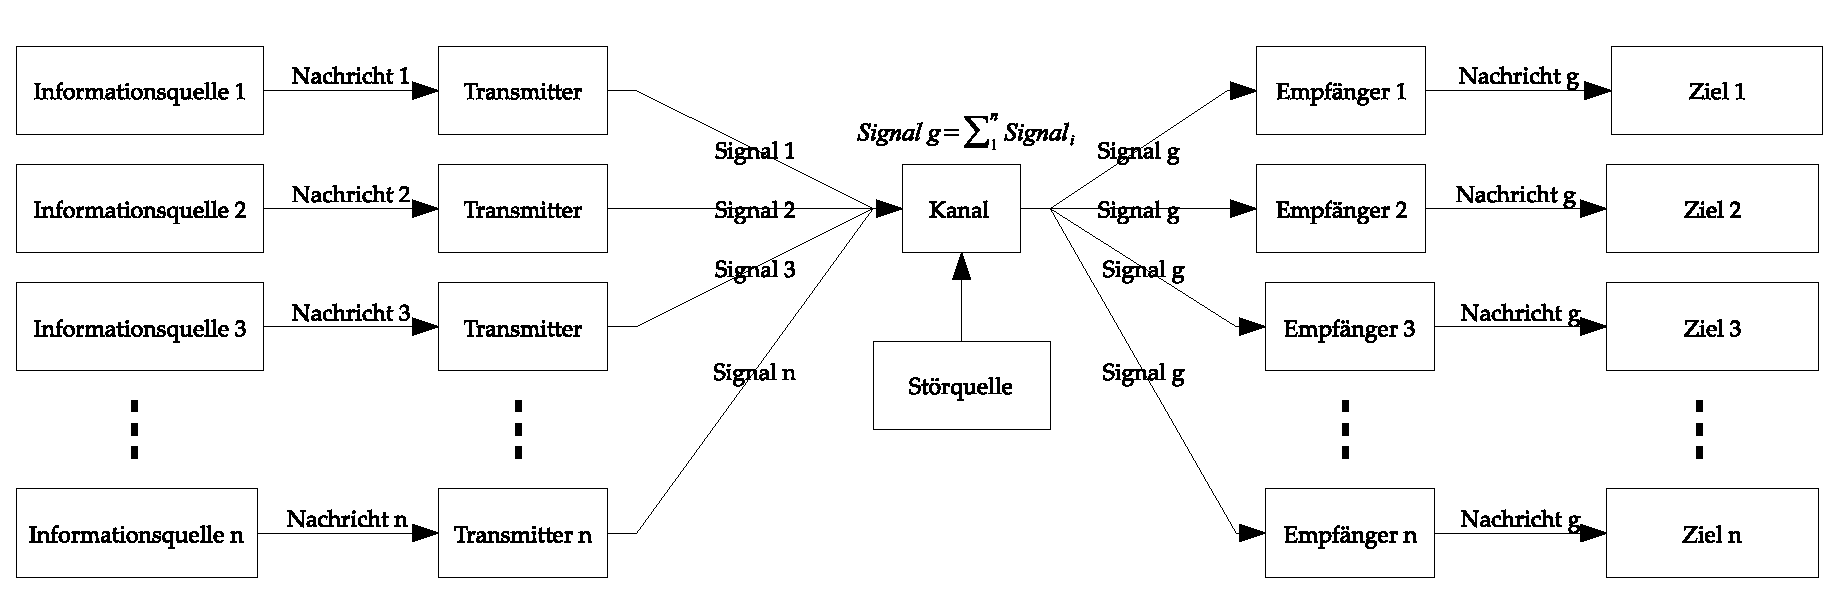
\includegraphics[width=1.00\textwidth]{grafiken/singlekanal-kommunikationsmodell.eps}
		\caption{Ein einziger Kanal b�ndelt alle �bertragenen Signale und f�hrt so zu Adressierungsproblemen}
		\label{fig:einkanalsystem}
\end{figure}

Ein Gro�teil der St�rungen resultiert aus der Untauglichkeit eines einzigen �ber\-tragungs\-kanals, mehrere gleichzeitige Audiostr�me zu transportieren. Dies f�hrt zu folgenden Hauptproblemen:

\begin{itemize}

	\item \textbf{Limitierter Kanal}: Existiert nur ein Kanal, der durch alle Spieler genutzt wird, k�nnen nur die wichtigsten Themen besprochen werden. Deswegen gebrauchen Teilnehmer diesen nur zur reinen aufgabenorientierten Koordinierung des Teams. Der gew�nschte soziale Aspekt der Kommunikation bleibt dagegen meist vollst�ndig aus. 
	
	\item \textbf{St�rungen durch Interferenzen}: Durch �berlagerung von mehreren gleichzeitigen Audiostr�men nimmt die Qualit�t des Mediums kontinuierlich ab, bis zu dem Punkt, an dem viele Spieler die Sprachkommunikation als st�rend empfinden.
	
		\item \textbf{Geringe Audioqualit�t}: Jede Audioquelle, die mit St�r\-ge\-r�u\-schen behaftet ist st�rt automatisch alle anderen Teilnehmer. Solche problematischen st�rungsbehafteten Audioquellen k�nnen nicht gemieden oder ausgeblendet werden.

	\item \textbf{Keine Kontrolle �ber Empf�nger der Nachricht}:  Bedingt durch die Massenkommunikation kann keine gezielte Adressierung der Teilnehmer erfolgen. So k�nnen auf einem Kanal nur alle Teilnehmer gleichzeitig angesprochen werden, und der Empf�nger konnte nur aus dem Kontext erkennen, dass die Nachricht f�r ihn bestimmt ist. 
	
		\item \textbf{Keine Kontrolle �ber Empfang der Nachrichten}: Analog zum Addressierungsproblem sind Teilnehmer genauso wenig in der Lage zu kontrollieren, welche Sprachnachrichten sie empfangen m�chten und welche sie verwerfen wollen. Oft f�hrt dies dazu, dass ein Gro�teil der Sprachkommunikation auf dem Kanal als L�rm empfunden wird. 
		
Ein Einkanalsystem hat aber auch einige Vorteile:

\begin{itemize}
	\item \textbf{Linear ansteigender Bandbreitenverbrauch}: Da der Audiostrom zentral gemischt wird, muss der Server der den Kanal betreibt, bei N Teilnehmern genau N Str�me entgegennehmen und nur N Audiostr�me verschicken. Dieses Verhalten wird genauer in Kapitel \ref{Architektur-Entwurf} behandelt.
	\item \textbf{Einfache Kanaladministration}: Existiert nur ein einziger Kanal, ist seine Administration und der Mischvorgang einfach. Alle Spieler die den Kanal betreten erhalten die Summe aller Signale und versenden auch ihr eigenes Signal an den Kanal.  
\end{itemize}

\end{itemize}
\begin{figure}[tbh]
	\centering	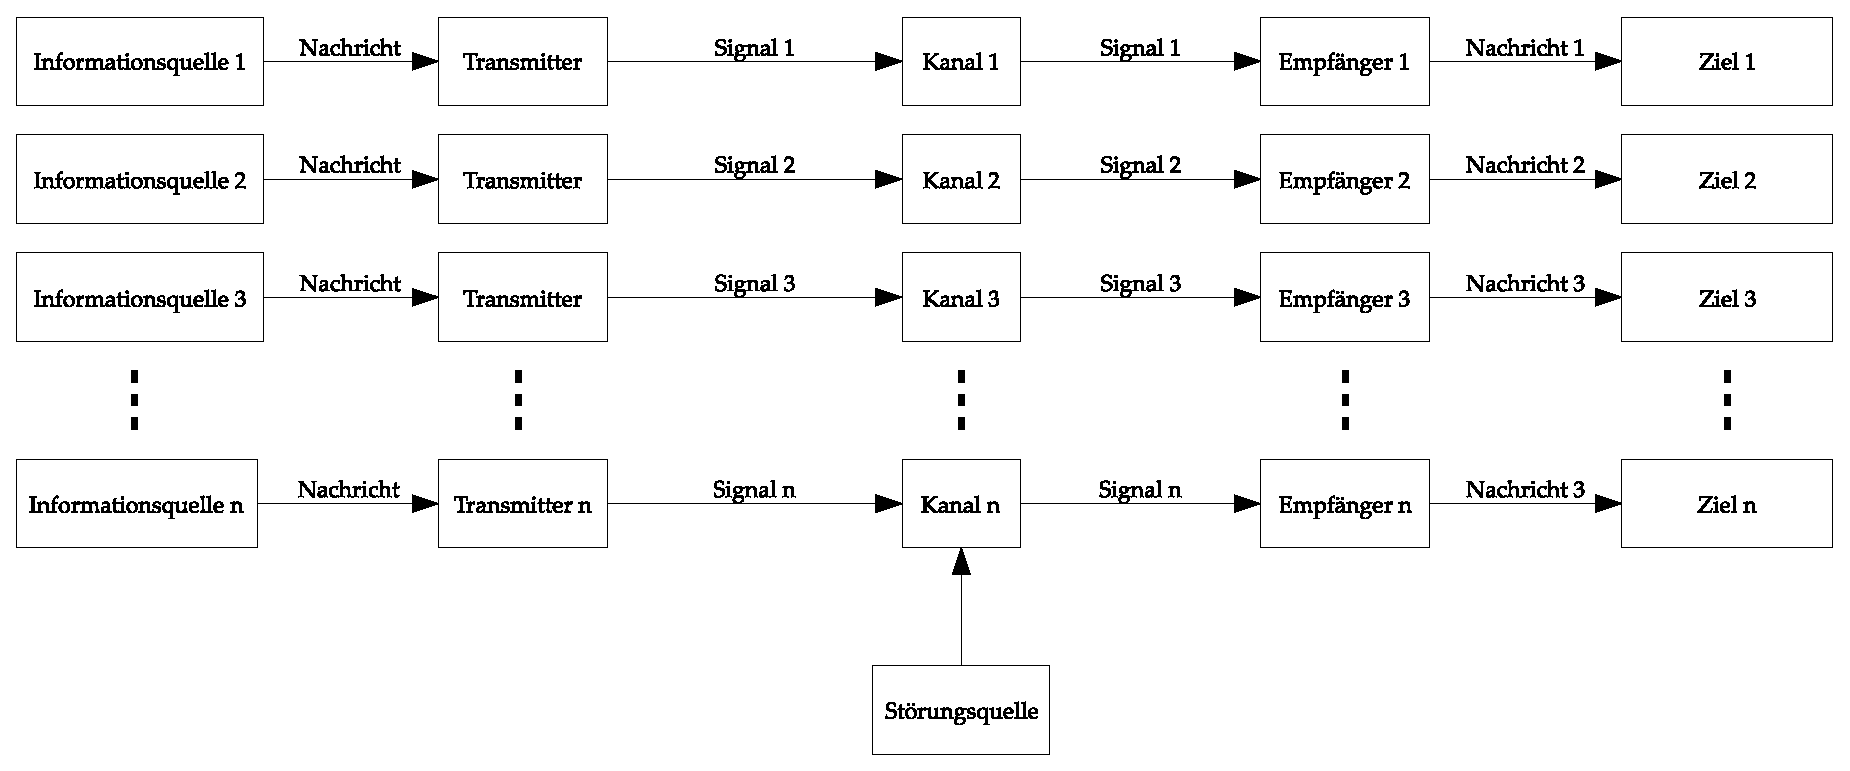
\includegraphics[width=1.00\textwidth]{grafiken/multi-kommunikationsmodell.eps}
	\caption{Einsatz von jeweils direkten Kommunikationskan�len zwischen Teilnehmern}
	\label{fig:mehrkanalsystem}
\end{figure}

Wird ein einziger Kanal durch mehrere parallele direkte Kan�le zwischen den Teilnehmern ersetzt (siehe Abbildung \ref{fig:mehrkanalsystem}), so k�nnen viele der genannten Probleme gel�st werden, indem jeder Spieler eine bessere Kontrolle �ber das Medium erh�lt. Er kann dann f�r jede Audioquelle selbst entscheiden, wie er mit ihr verfahren will. 

\begin{itemize}
	\item  Wird zwischen jedem Spielerpaar jeweils ein Kanal genutzt, k�nnen keine Interferenzen durch �berlagerungen von Audioquellen auftreten.
	\item Jeder Spieler ist genau in der Lage zu entscheiden, an wen seine Nachricht gehen soll, da f�r jede �bertragung jeweils ein Kanal benutzt wird. 
	\item Da jedes empfangene Audiosignal den Empf�nger ungemischt erreicht, ist dieser in der Lage unerw�nschte Signale auszufiltern.
	\item Findet das Abmischen der Kan�le lokal statt, kann so eine hohe Qualit�t des Mischsignals gew�hrleistet werden.	
	\item Der Spieler ist im Stande so viele pers�nliche Gespr�che zu f�hren wie er m�chte, ohne die ganze Gruppe zu st�ren.
\end{itemize}

In diesem Modell kann auch das Feedback entsprechend dem Modell von Schramm \cite{schramm54} gezielt erfolgen, indem es immer nur an die entsprechende Person erfolgt und nicht mehr an alle Teilnehmer des Spiels.
 
Es resultieren auch einige - vor allem technische Nachteile aus der Verwendung von mehreren Kan�len, die hier nicht unerw�hnt bleiben sollen, jedoch erst in Kapitel \ref{Architektur-Entwurf} detailliert behandelt werden.

\begin{itemize}
	\item \textbf{Kanaladministration}: Da f�r jede Audioverbindung ein separater Kanal benutzt wird, muss auf Clientseite eine ausgefeilte Steuerung daf�r sorgen, dass der Spieler mit den richtigen Kan�len verbunden wird. Mit genau diesem Problem befasst sich das Unterkapitel \ref{proxemikalssteuerungvonkonferenzen}.	
	\item \textbf{Quadratisch ansteigender Bandbreitenverbrauch}: Da der Audiostrom von jedem Teilnehmer lokal gemischt wird, muss auch jeder Teilnehmer alle anderen Audiostr�me empfangen und seinen Audiostrom an alle Teilnehmer verschicken. 
\end{itemize}
 
\section{Gleichzeitige interpersonelle und Massenkommunikation}

Die fehlende Unterscheidung in eine interpersonelle und Massenkommunikation resultiert auch aus der Benutzung eines einzigen Kanals f�r alle Teilnehmer. Spieler k�nnen ihre Nachrichten nur an alle Benutzer des Kanals senden, da der einzige �bertragungsmodus oft nur die Massenkommunikation ist. Jeder Teilnehmer des Kanals h�rt s�mtliche Konversationen der Mitglieder und hat keinen Einfluss darauf, ob er manche Teilnehmer nicht h�ren m�chte. 

Dies f�hrt dazu, dass das Medium stark reglementiert werden muss und nur die allerwichtigsten Informationen �ber den Kanal ausgetauscht werden. In der Praxis werden oft auch so genannte \textit{Channel Leader} (siehe Abbildung \ref{fig:ventrillo}) ernannt, die �ber Sprachrechte verf�gen w�hrend alle anderen Spieler nur zuh�ren k�nnen. 

Es ist prinzipiell zwar m�glich, dass Teilnehmer auf dem Kanal ein pers�nliches Gespr�ch f�hren. Dieses Verhalten wird aber nicht gerne von anderen Teilnehmern gesehen, wie Studien in aus Kapitel 2 gezeigt haben. Deswegen verf�gen einige Hilfsprogramme\footnote{Blizzard Entertainment: World of Warcraft Communication Basics, Version 22.03.2008, http://worlfofwarcraft.com/info/basics/voicechat.html} �ber einen "`Fl�stermodus"', der eine private Konversation mit einzelnen Spielern erm�glicht. Eine solche Verbindung muss jedoch bereits vor der Teilnahme am eigentlichen Spiel in der Konfiguration des Hilfsprogramms definiert werden. Somit ist ein spontanes Gespr�ch mit einem beliebigem Spieler deshalb nicht ohne weiteres m�glich. Zudem werden Teilnehmer eines solchen "`Fl�stergespr�chs"' vom restlichen Geschehen ausgegrenzt, da sie nicht gleichzeitig beide Kan�le benutzen k�nnen.

\begin{figure}[tbh]
	\centering
		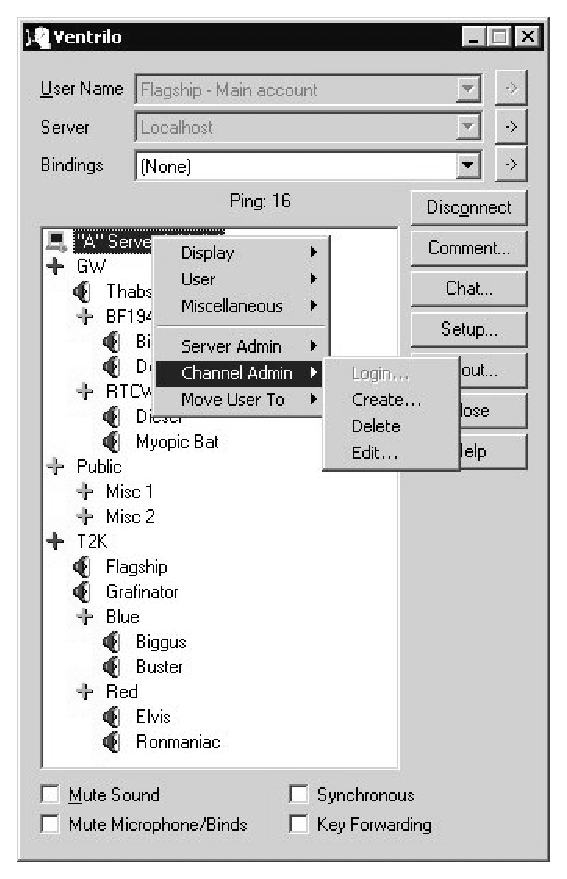
\includegraphics[width=0.40\textwidth]{grafiken/ventrillo.eps}
		\caption{Konfiguration von Kan�len, Gruppen und Rechten in kommerziellen Sprach\-kommunikations\-programmen}
	\label{fig:ventrillo}
\end{figure}

Der Verbesserungsvorschlag sieht vor, dass Teilnehmer sowohl pers�nliche Gespr�che f�hren k�nnen, als auch an der Massenkommunikation teilnehmen k�nnen. Dies soll durch einen erweiterten Mischvorgang erm�glicht werden, der die Teilnahme an einem Kanal nicht bin�r definiert, sondern einen flie�enden �bergang zwischen Kan�len erm�glicht.

\section {Erweitertes Audio Mixing}
Da bisher die Teilnahme an einer Konferenz bin�r gel�st wurde, waren Spieler entweder Teil einer solchen oder nicht. So ist das in einer Konferenz mit \textit{n} Teilnehmern ${p_{1},p_{2},...,p_{n}}$, mit Audiostr�men ${V_{1}(t),V_{2}(t),...,V_{n}(t)}$, von einem Teilnehmer $i$ zu einer Zeit \textit{t} empfangene Signal $R_{i}(t)$ aller Teilnehmer $j$ definiert durch:

\begin{align}
	R_{i}(t) = \sum \limits_{j=1}^n {V_{j}(t)}  \ \ \mbox{wobei} \  1 \geq j \geq n \ \mbox{und} \  j \neq i
\end{align}

Der Verbesserungsvorschlag sieht vor den bin�ren Teilnahmestatus durch eine stetige Teilnahmefunktion zu ersetzen.  Die Teilnahme an einer Konferenz soll von der Distanz $d_{j}$ zum anderen Teilnehmer abh�ngig sein und somit alle Werte zwischen 0 und 1 annehmen. Das empfangene Signal $R_{i}(t)$ wird somit definiert als:

\begin{align}
	R_{i}(t) = \sum \limits_{j=1}^n {d_{j} \cdot V_{j}(t)} \ \ \mbox{wobei} \ 1 \geq j \geq n \ \mbox{und} \ j \neq i
\end{align}

In einer 3D Umgebung, in der die Spieler beliebige Positionen zueinander einnehmen k�nnen, wird vom Spieler ein Distanzvektor zu den �brigen Spielerpositionen berechnet und die Lautst�rke des entsprechenden Audiostroms anhand diesem angepasst. Ein solcher Ansatz erm�glicht es f�r den Spieler eine eigene Konferenz zu erstellen, in der die Teilnehmer nur zu einem bestimmten Prozentsatz, repr�sentiert durch ihre Lautst�rke, anwesend sind. 

Personen die sich in der N�he befinden sind besser zu h�ren, als Personen die sich weit entfernt befinden. Die Kontrolle der Konferenz findet somit nicht direkt durch Tastatureingaben statt, sondern h�ngt implizit von der Position und Bewegung der Spieler zueinander ab. Um dieses Mixingkonzept zu realisieren, wird das Modell der Proxemik eingesetzt, das bereits im zweiten Kapitel vorgestellt wurde und dessen Implementierung in Kapitel 7 besprochen wird.

%\section{Hohe Mediarichness}
%Wie Studien der Texkommunikation gezeigt haben, besteht ein gro�es Interesse nach einem Medium f�r Kommunikation in Spielen, das eine ausreichend hohe Mediarichness besitzt. 
%Textkommunikation dagegen enth�lt au�er der urspr�nglichen Nachricht viele Akronyme und Emoticons, die nur unzul�nglich die soziale Komponente einer Kommunikation widerspiegeln k�nnen und ist f�r durch die Nutzung von eines einzigen gemeinsamen �ffentlichen Kommunikationskanals nicht f�r pers�nliche Gespr�che tauglich. 

%Dabei besteht gerade f�r die pers�nliche soziale Kommunikation �ber\-proportio\-naler Bedarf, wie Studien aus Kapitel 2 festgestellt haben. Die Vermutung liegt nahe, dass die Spieler die Handicaps der Textkommunikation zwar teilweise erfolgreich durch verschiedene Methoden behoben haben, trotzdem der Wunsch nach einem Medium, das besser ohne Einschr�nkungen in der Lage ist Nachrichten sozialer Natur zu �bertragen nach wie vor vorhanden ist und auch eingesetzte Tools bisher dieser Aufgabe nicht gerecht werden. Dies entspricht auch Beobachtungen der Media-Richness Theorie, nach der komplizierte Telekoordinationsaufgaben ein ebenso reiches Medium ben�tigen.

%Spielen kann als  Kooperationsaufgabe mit einer Vielzahl an Teilnehmern und komplexen Anforderungen in Bezug auf die Gruppendynamik und das Timing verstanden werden. Sprachkommunikation scheint genau den Grad an Mediarichness zu besitzen die Spiele ben�tigen. Sie erlaubt kurze Feedbackzeiten, was die Interaktivit�t f�rdert und ist durch verschiedene Stimmvariationen lebendig genug um Emotionen wie z.B. Wut und Freude auszudr�cken. 

% Daraus ergibt sich das Ziel, dass die Sprachakommunikation so umgesetzt werden soll, dass sie Teilnehmern eine zum einen durch ihre Art eine bessere Koordination erm�glicht, gleichzeitig aber intuitiv bedient werden kann um eine "`overcomplication"' \cite{reichswald98} zu vermeiden. 
%TODO BIld einer "`klassischen Sprachkommunikation mit Konfigurationen"'
%\begin{table}
%\centering
%\caption{Eine Gegen�berstellung der Media-Richness Eigenschaften von Sprache und Text}
%\begin{tabular} {p{0.3\textwidth}p{0.3\textwidth}p{0.3\textwidth}}
%			\toprule
%			\textbf{Merkmale} & \textbf{Sprache} & \textbf{Text} \\
%			\midrule
%			Feedback & direkt	& mit Verz�gerung	
%			\tabularnewline [7 pt]
%			Anzahl der Kommunikationskan�le & viele Sprachkan�le & ein gemeinsamer Chat\-raum
%			\tabularnewline [7 pt]
%Pers�nliche \newline unpers�nliche Sprache & �bermittlung von Emotionen m�glich &  nur mit Emoticons m�glich 
%			\tabularnewline [7 pt]
%			Vielfalt der verwendeten Sprache & ausdrucksstark & oft nur Abk�rzungen \\
%			\bottomrule
%		\end{tabular}
%\end{table}


%Bild von Schall in Luft.

\section{Proxemik als Steuerung von Konferenzen}
\label{proxemikalssteuerungvonkonferenzen}
Obwohl die Verwaltung von Telefonkonferenzen seit Jahren erforscht wird, \cite{schulzrinne02}, existieren bisher wenige intuitive Methoden zu ihrer Steuerung. Alle Studien zur Konferenzsteuerung zeigen, dass die Einf�hrung von mehreren Kan�len ein entsprechend kompliziertes Konferenz-Management (siehe Abbildung \ref{ventrillo} erfordert, da Teilnehmer in der Lage sein m�ssen, zu entscheiden was sie h�ren wollen und was nicht. 

Die in der Arbeit vorgeschlagene L�sung besteht aus der Reduzierung dieses Problems zu einem Nachbarschaftsproblem, in dem Spieler durch ihre Distanz zueinander entscheiden k�nnen welche Kan�le sie h�ren m�chten und welche nicht. 

%Es entscheidet einzig die Entfernung der Teilnehmer zueinander, ob eine interpersonelle oder Massenkommunikation gew�nscht wird. Jeder Teilnehmer ist so in der Lage intuitiv seine pers�nliche Konferenz zu erstellen. 

Nonverbale Kommunikation in Form der Bewegung der Avatare, tr�gt somit nicht nur zur Erh�hung der Interaktivit�t und Lebhaftigkeit bei, sondern bildet die Grundlage f�r die einfachste und intuitivste Form der Steuerung einer Konferenz.

Durch die Repr�sentation der Konferenzteilnehmer durch Avatare im 3D-Raum, kann jeder selbst bestimmen welche Entfernung er zum Nachbarn einnehmen will. Diese entscheidet wie im realen Leben, ob er jemanden h�rt oder nicht. 

Im besonderen bedeutet es, dass der Raum um den Spieler in drei Distanzzonen eingeteilt wird, in denen verschiedene Auspr�gungen der Sprachkommunikation m�glich sein sollen. Dieser Vorschlag ist angelehnt an die Proxemikforschung \cite{hall05}, deren Grundlagen aufgegriffen und neu interpretiert werden. Eine Ausf�hrliche Beschreibung der technischen Vorg�nge in diesen Zonen findet sich in Absatz \ref{Zonen-Implementierung}. 

\begin{itemize}
	\item \textbf{Pers�nliche Distanz}: Hier sollen Spieler in der Lage sein pers�nlich miteinander zu kommunizieren. Vorstellbar sind drei Alternativen:
	\subitem[$A_{1}$] Ein Gespr�ch dieser Distanzzone kann ausschlie�lich von den 2 Teilnehmern geh�rt werden.
	\subitem [$A_{2}$] Das Gespr�ch dieser Zone besitzt eine f�r den Teilnehmer gr��ere Lautst�rke als alle anderen Gespr�che.
	\subitem [$A_{3}$] Das Gespr�ch dieser Zone verf�gt �ber eine bessere Sprachqualit�t, als alle anderen Gespr�che.
	
	\item \textbf{Soziale Distanz}: Hier soll die direkte Entfernung der Spieler untereinander Einfluss auf die wahrgenommene Lautst�rke haben. Spieler die sich n�her befinden sollen lauter h�rbar sein, w�hrend Spieler die sich weiter entfernt befinden leiser h�rbar sein sollen. Die Lautst�rke soll vom inneren Radius bis zum �u�eren Radius der Zone linear abnehmen, bis Spieler die �ffentliche Zone erreichen und nicht mehr h�rbar sind. Dies Verhalten entspricht dem erweitertem Mixing Konzept und simuliert gleichzeitig die �bertragung der Sprache durch die Luft.
	
	\item \textbf{�ffentliche Distanz}: In der �ffentlichen Distanz ist keine weitere Sprachkommunikation m�glich. Das einzige Mittel bleibt hier die Textkommunikation, die jederzeit und an jeden Spieler �bertragen wird, und somit dem �ffentlichen Charakter der Zone entspricht. Damit der �bergang von der �ffentlichen Zone zur sozialen Zone st�rungs- und verz�gerungsfrei ablaufen kann, soll hier eine Grundkonnektivit�t aufgebaut werden:  Die Verbindung zwischen den Teilnehmern wird auf Protokollebene aufgebaut, um dann in der sozialen Zone direkt verf�gbar zu sein. 
	
\end{itemize}

\begin{figure}[tbh]
	\centering
		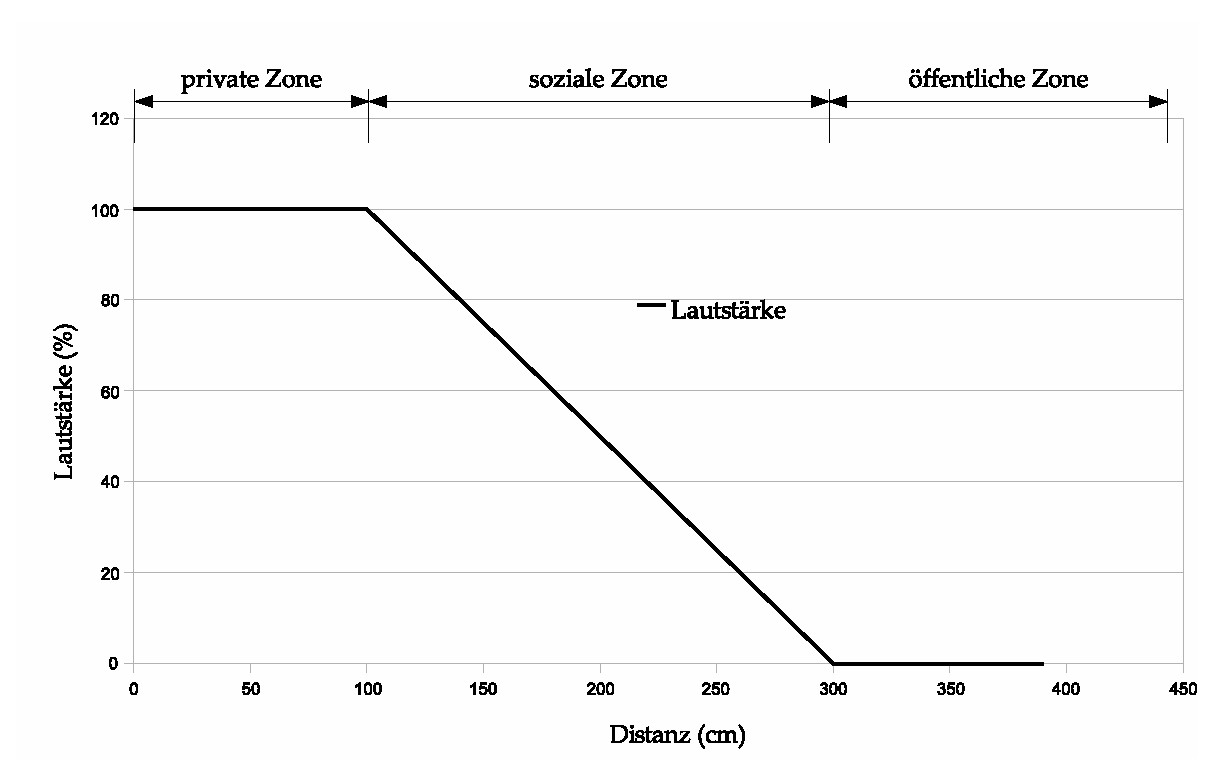
\includegraphics[width=1.00\textwidth]{grafiken/lautstaerke.eps}
		\caption{Distanzbasierte Ver�nderung der Lautst�rke in Abh�ngigkeit der gew�hlten Zone}
	\label{fig:lautstaerke}
\end{figure}

\begin{sloppypar}
Bevor jedoch eine konkrete Umsetzung erl�utert wird werden im darauf folgenden Kapitel Grundlagen im Bereich der IP-Telefonie vermittelt.	
\end{sloppypar}

\newpage~
\chapter{VoIP Grundlagen}

Voice-over-IP (auch VoIP, IP-Telefonie) bezeichnet die Telefonie �ber das Internet oder Computernetzwerke. Um per VoIP ein Telefongespr�ch f�hren zu k�nnen, ben�tigen Benutzer ein software-basiertes SIP-Telefon oder VoIP-Telefon-Hardware. Gespr�che sind mit jedem beliebigen Teilnehmer m�glich: Sowohl VoiP-Nummern als auch Teilnehmer mit normalen Telefonnummern k�nnen angerufen werden.

\section{Protokolle zur Echtzeitkommunikation}
	Voice-over-IP beinhaltet unterschiedliche Protokolle. Zur reinen Signalisierung werden haupts�chlich das Session Initiation Protocol (SIP) \cite{sip02} bzw. Protokolle aus der H.323-Protokollfamilie\footnote{Da SIP die �ltere H.323 Protokollfamilie abl�st, wird diese hier nicht behandelt.} verwendet. Bei VoIP sind generell folgende Klassen der Protokolle zu unterscheiden:
\begin{itemize}
	\item Protokolle f�r die Sprach�bermittlung: Da die Sprachkommunikation in Echtzeit verl�uft, sind spezielle Protokolle f�r die �bermittlung der Sprache �ber IP-Netze n�tig.
	\item Signalisierungsprotokolle: Es handelt sich hier um Protokolle f�r den Auf- und Abbau von Verbindungen zwischen IP-Telefonen.
\end{itemize}

F�r die Signalisierung werden das Session Description Protocol (SDP)\cite{sdp98} und das Session Initiation Protocol (SIP) eingesetzt. Diese �bernehmen die Vermittlung von Gespr�chen, den Rufauf- oder -abbau, sowie die Aushandlung von Parametern. Die Verwendung eines gemeinsamen Codecs, der entsprechenden Bitrate oder der maximal zul�ssigen Bandbreite werden in diesen Protokollen kontrolliert. 

F�r die Sprach�bertragung wird das Echtzeit Transport Protokoll (Realtime Transport Protocol (RTP)) \cite{rtp96} ver\-wen\-det, das dem Empf�nger der Pakete erlaubt, trotz unzuverl�ssiger �bertragung �ber UDP \cite{udp80}, einen Paketverlust festzustellen und die urspr�ngliche Reihenfolge der Daten wiederherzustellen. RTP ist nicht nur f�r Sprache, sondern auch f�r alle anderen Echtzeitmedien, wie Video verwendbar. Da RTP keine Kontrollinformationen versendet, kann der Empf�nger dem Sender nicht mitteilen, ob �berhaupt bzw. wie die Sprache in Form von IP-Paketen bei ihm ankommt. Das RTP Control Protocol (RTCP) \cite{rtcp03} gleicht diesen Nachteil aus: Mit Hilfe von RTCP k�nnen zus�tzlich zu den reinen Mediendaten auch Kontrollinformationen, wie die Anzahl der verlorenen Pakete oder der gemessene Jitter der RTP-Verbindung �bertragen werden und so �bertragungsparameter angepasst werden. 

\begin{figure}[tbh]
	\centering
		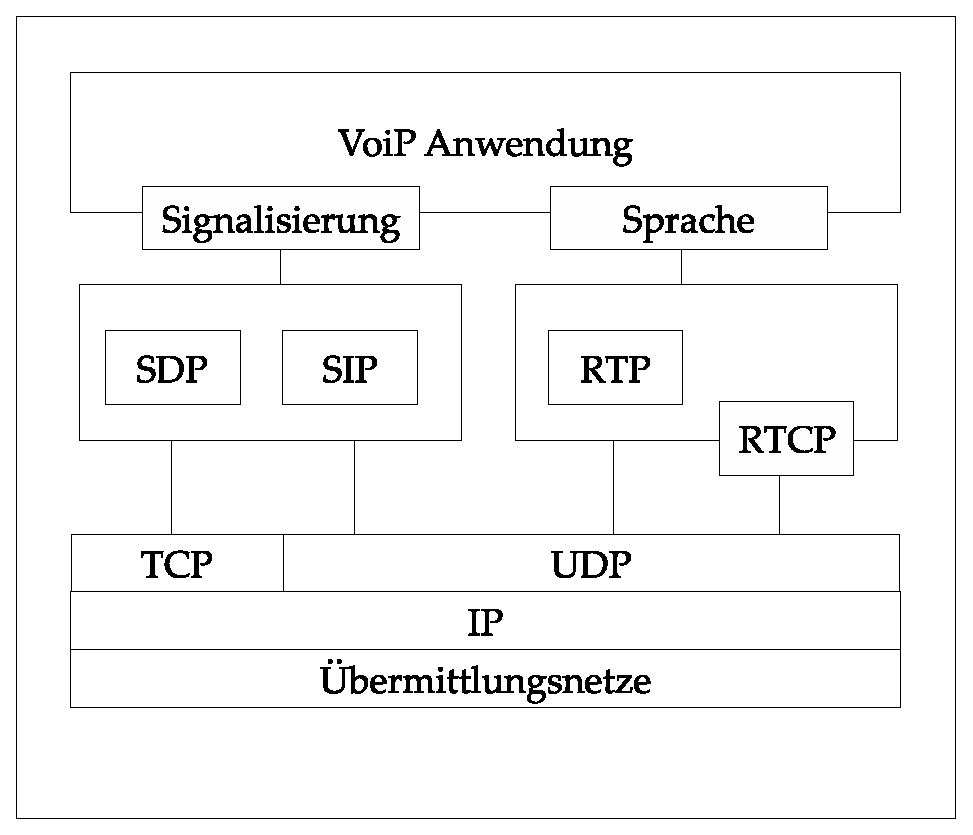
\includegraphics[width=.60\textwidth]{grafiken/voipprotokolle.eps}
	\caption{Eine �bersicht �ber die VoIP Protokollfamilie}
	\label{fig:voipprotokolle}
\end{figure}

%Neben den bisher erw�hnten Protokollen zur Hauptfunktionalit�t gibt es noch noch wei\-te\-re, die sich mit allen angrenzenden Bereichen von VoIP besch�ftigen. So wird mit Hilfe des STUN (Simple Traversal of User Datagram Protocol Through Network Address Translators) \cite{stun03} erm�glicht seine IP-Adresse zu ermitteln, falls man sich hinter einem NAT Router befindet und die interne IP-Adresse nicht der externen entspricht. Dies ist vor allem notwendig, da die IP-Kontakt\-in\-for\-mationen in SIP und SDP in der Anwendungsschicht �bertragen werden und somit ein Client ohne Kenntnis richtigen Adresse falsche Informationen liefern w�rde. Ein weiteres Protokoll mit dem Ziel der �berbr�ckung eines NATs ist TURN(Traversal Using Relay NAT) \cite{turn08}. Bei TURN bekommt ein Client von einem TURN-Server eine �ffentlich erreichbares IP-Adressen- und Port-Paar zugewiesen und leitet alle an diese �ffentliche Adresse ankommenden Pakete an den Client weiter. 

%F�r die Ansteuerung von VoIP-Gateways stehen die Protokolle MGCP(Media Gateway Control Protocol) \cite{mgcp99} und Megaco (Media Gateway Control) \cite{megaco00} zur Verf�gung, die im Rahmen der Arbeit jedoch nicht weiter erl�utert werden. 

%Dieses Kapitel soll zun�chst den Aufbau eines VoIP Systems beschreiben um anschlie�end die Protokolle SIP, SDP, RTP und RTCP zu behandeln. Da SIP die �ltere H.323 Protokollfamilie in langfristig verdr�ngen wird, wird diese nicht behandelt. %Im Abschluss wird ein �berblick �ber das propri�tere Protokoll von Skype gegeben, dessen Funktionsweise und Details zwar nicht offen sind, es jedoch eine Alternative zu den offenen Protokollen bietet. 

\subsection{Einfaches VoIP System}
Der einfache Aufbau eines funktionierenden VoIP Systems kann prinzipiell mit einer bestehenden IP-Infrastruktur und Computerprogrammen, die Telefonie erm�glichen (\textit{Softphones}), funktionieren. Die Teilnehmer m�ssen jedoch bei einer solchen Konfiguration die IP-Adressen der gew�nschten Ge\-spr�chs\-partner kennen, um einen direkten Anruf auszuf�hren. Bei einer Adress\-�nderung der IP Adresse eines Gespr�chspartners, m�ssten jedoch alle Eintr�ge der Gespr�chspartner entsprechend abge�ndert werden, weil sich die Teilnehmer sonst nicht mehr erreichen k�nnten. Der gleiche Aufwand m�sste auch beim Hinzuf�gen weiterer Teilnehmer erfolgen. %Ein solcher Aufbau wird daher als unflexibel angesehen. 

Im SIP-Protokoll wird dieses Problem von Komponenten (\textit{Proxys}), die die Aufgabe einer Vermittlungsstelle einnehmen, �bernommen. Ein Proxy kann einen Lokationsdienst(\textit{Location Service}) enthalten, der ankommende SIP-Pakete an das Telefon des angerufenen Teilnehmers weiterleitet oder an einen anderen Proxy weiterleitet, falls sich der Benutzer au�erhalb des eigenen Adressbereichs befindet. Zus�tzlich k�nnen Konferenzen, Voice-Mail und Anrufweiterleitungen Teil eines VoIP Systems sein. 

%Da die klassische Telefonie weiterhin neben VoIP Bestand hat, wird versucht mit zus�tzlichen Komponenten, den Gateways, eine Verbindung zwischen den beiden Telefonsystemen herzustellen. 


\subsection{Einflussfaktoren auf die VoIP-Qualit�t}
Die wichtigsten \textit{Quality-of-Service}-Anforderungen, die VoIP an IP-Netze stellt, betreffen:
\begin{itemize}
	\item die Bandbreite von virtuellen Verbindungen zwischen IP-Telefonen,
	\item die Ende-zu-Ende-Verz�gerung des Sprachsignals (Delay),
	\item die Schwankung der �bermittlungszeit (Jitter) und
	\item die Paketverlustrate (Packet Loss Rate)
\end{itemize}

\subsubsection{Bandbreite}
Da bei VoIP die Sprache zuerst digitalisiert und dann entsprechend codiert wird, ist dabei die Qualit�t des �bertragenen codierten Sprachsignals abh�ngig von der Bandbreite f�r die virtuelle Verbindung zwischen den IP-Telefonen. Dabei k�nnen die eingesetzten Sprachcodecs sich in ihren Bitraten stark unterscheiden, wie eine �bersicht in der Tabelle \ref{pt-tabelle} zeigt. Die Bitrate sollte geringer als die vorhandene Bandbreite gew�hlt werden, da ansonsten nicht alle Pakete �bertragen werden k�nnen und St�rungen auftreten.

\subsubsection{Ende-zu-Ende-Verz�gerung (Delay)}
Unter der Ende-zu-Ende-Verz�gerung des Sprachsignals versteht man die Zeitspanne, die ein Sprachsignal vom Mund eines Sprechers bis zum Ohr eines H�rers ben�tigt. Die Ende-Zu-Ende-Verz�gerung entsteht vor allem durch die Zwischenspeicherung der IP-Pakete in den Routern, die sie auf ihren Wegen durch das Netz zu durchlaufen haben. Jeder Router ben�tigt Zeit, um den Header im IP-Paket zu interpretieren und die entsprechende Routing-Entscheidung zu treffen. Trifft ein Paket unterwegs auf einen �berlasteten Router, muss es einige Zeit in der Warteschlange vor der Leitung verbringen und wird im Extremfall sogar ganz verworfen. Eine gro�e Ende-zu-Ende-Verz�gerung beeintr�chtigt den Charakter eines Telefongespr�ches stark. 

Da die Sprachkommunikation in Echtzeit verl�uft, gilt die Wiedergabe eines Sprachsignals am Ziel als qualitativ schlecht, wenn sie einem zu gro�en Zeitverzug erfolgt. F�r die Ende-zu-Ende-Verz�gerung $T_{EE}$(End-to-End-Delay) des Sprachsignals werden daher Grenzwerte gesetzt. Nach dem ITU-T-Dokument G.114 wird die VoIP-Qualit�t wie flogt klassifiziert:
\begin{itemize}
	\item $T_{EE}$ kleiner als 150ms: akzeptabel f�r alle Benutzer,
	\item $T_{EE}$ zwischen 150ms und 300ms: akzeptabel, aber mit Einschr�nkungen (nicht f�r empfindliche Benutzer), 
	\item $T_{EE}$ gr��er als 300ms: nicht akzeptabel. 
\end{itemize}

\subsubsection{Schwankung der �bermittlungszeit (Jitter)}
Da die einzelnen IP-Pakete auf einer Verbindung zwischen IP-Telefonen auf unterschiedlichen Wegen �bermittelt werden, kann ihre �bermittlungszeit divergieren. Die Schwankungen der �bermittlungszeit werden Jitter genannt. Die \textit{Synchronit�t} dh. die zeitlich konstante Frequenz der �bertragenen Signale bei VoIP l�sst jedoch kein Jitter zu. Um die Schwankungen auszugleichen, wird beim Empf�nger ein spezieller Puffer verwendet. Man bezeichnet einen derartigen Puffer als Jitter-Ausgleichspuffer (\textit{Playout Buffer}).

\subsubsection{Paketverlustrate (Packet Loss Rate)}
Die Verluste von IP-Paketen mit Sprache w�hrend der �bermittlung mindern die Qualit�t. Die Anzahl der Paketverluste in einer bestimmten Zeitperiode wird mit dem Parameter Paketverlustrate angegeben. Paketverluste k�nnen durch �berlastete Router im IP-Netz oder auch durch einen "`schlecht"'  dimensionierten Jitter-Ausgleichspuffer entstehen. Im Gegensatz zu reinen Datenanwendungen, ist der Verlust eines IP-Pakets bei der Sprach�bertragung nicht besonders tragisch. Zu viele Paketverluste jedoch machen sich in einem Telefongespr�ch allerdings sehr st�rend als Unterbrechungen bemerkbar. 

\subsection{VoIP-relevante Sprachkodierungsverfahren}

%TODO enter all Codecs
%\cite{speex08}

Obwohl die Qualit�t der Sprach�bertragung durch Parameter, wie die Laufzeit der IP-Pakete (Delay), die Laufzeitunterschiede(Jitter) und die Verlustrate von IP-Paketen im Netz (Packet Loss) beeinflusst wird, sagen diese Parameter nichts �ber die eigentliche Sprachqualit�t aus. Diese wird nach der MOS (Mean Opinion Score) \cite{mtu96} - Skala  gemessen. Sie unterscheidet Aspekte wie Verst�ndlichkeit der Sprache, Akzeptanz der Lautst�rke sowie die Akzeptanz der Laufzeitschwankungen und Echos. 

%TODO Tabelle mit Codecs
\begin{table}[tbh]
	\centering
		\begin{tabular}{p{0.2\textwidth}|p{0.6\textwidth}}
		\toprule
		\textbf{MOS-Wert} & \textbf{Bedeutung} \\
		\midrule
		5=excellent & keinerlei Anstrengung zum Verst�ndnis der Sprache notwendig; totale Entspannung m�glich \\
		\hline
		4=good & keine Anstrengung notwendig, Aufmerksamkeit n�tig \\
		\hline
		3=fair & leichte, moderate Anstrengung n�tig \\
		\hline
		2=poor & merkbare, deutliche Anstrengung n�tig \\
		\hline
		1=bad & trotz Anstrengung keine Verst�ndigung \\
		\bottomrule
		\end{tabular}
\end{table}

Eine analoge Sprach�bertragung kommt auf einen MOS-Wert von 3.5 bis 4. Hochwertige VoIP-Implementierungen bieten eine Sprachqualit�t zwischen 3.8 und 4.4 je nach verwendeter Sprachkodierung. Dabei bieten VoIP-Systeme mindestens die Qualit�t eines herk�mmlichen analogen Telefonnetzes. 

Es gibt mehrere Sprachkodierungsverfahren, die bei Voice over IP verwendet werden k�nnen. Man unterscheidet zwischen abtastwert-orientierten Kodierungsverfahren, die zwar gute Sprachqualit�t garantieren aber Bitraten haben, die gr��er als 16 Kbit/s sind und segment-orientierten Kodierungsverfahren die zwar geringe Bitraten haben aber daf�r nur eine schwache bis gute Sprachqualit�t bieten. Eine �bersicht �blicher Codecs findet sich in Tabelle \ref{pt-tabelle}.

\begin{table}
\centering
\caption{Einige Sprachkodierungsverfahren ihre PT-Nummern und Bitraten}
\label{pt-tabelle}
\begin{tabular}{lllr}
\toprule
PT-Nr. & Kodierungsname & Kodierungsart & Bitrate (kbit/s) \\
\midrule
0  & PCM $\mu-Law$ & Abtastwert-orientiert & 64 \\
4  & G723 & Segment-orientiert & 5.3-6.3 \\
8 & PCM A-Law & Abtastwert-orientiert & 64 \\
12  & QCELP & Segment-orientiert & 4.8-6.8\\
15  & G728 & Segment-orientiert & 16\\
18  & G729 & Segment-orientiert & 8\\
dyn & G726-32 & Abtastwert-orientiert & 32 \\
dyn & G726-16 & Abtastwert-orientiert & 16 \\
\bottomrule
\end{tabular}
\end{table}

\section{Session Initiation Protokoll (SIP)}
Das \textit{Session Initiation Protocol} wurde zuerst im Jahr 1999 als RFC 2543 eingef�hrt und im Jahr 2002 in den RFCs 3262-3265 weiter spezifiziert. Das SIP Protokoll erm�glicht es zwischen kommunizierenden Rechnern �ber ein IP-Netz eine Sitzung (\textit{Session}) f�r die �bermittlung von Echtzeitmedien aufzubauen. Die Session stellt einen logischen Kanal dar, �ber den die Echtzeitmedien mit Hilfe des RTP Protokolls transportiert werden. SIP definiert bestimmte Nachrichten f�r den Auf- und Abbau von Sitzungen, ist einfach konzipiert und f�r Menschen leicht lesbar, da es in Anlehnung an das Internet Protokoll HTTP entwickelt worden ist. 

\subsection{SIP Komponenten}
% �ber komponenten eines SIP Systems schreiben
In der Architektur sind folgende Systemkomponenten definiert:
\begin{itemize}
	\item User Agent
	\item Proxy Server
	\item Redirect Server
	\item Registrar
\end{itemize}

Obwohl zwischen den Komponenten unterschieden wird, k�nnen sie alle in einem Rechner untergebracht werden oder auf verschiedene Computer verteilt werden. Eine typische Konfiguration sieht vor, dass in ein SIP Server die Proxy- und Registrarkomponentene enth�lt, w�hrend der Clients nur �ber den User Agent verf�gen.

\textbf{User Agent (UA):}User Agents sind alle SIP-f�higen Endger�te. Diese sind SIP-Telefone, Softphones oder andere Anwendungen und Hardware, die nach dem SIP Protokoll kommunizieren. Dabei besteht ein UA intern aus einem User Agent Client (UAC), der Anfragen mittels Nachrichten stellt und einem User Agent Server (UAS), der Anfragen entgegen nimmt. F�r die einfachste Form des Verbindungsaufbaus gen�gen zwei User Agents. Wobei jeder der UAS jeweils ein UAS und UAC sein kann. 

\textbf{Proxy Server:} Proxy Server dienen prim�r dem Routing und der Weiterleitung der SIP-Nachrichten. Zwischen zwei UA k�nnen beliebig viele Proxy Server liegen. Proxy Server k�nnen Rechtemanagement durchf�hren und ermitteln ob ein Benutzer berechtigt ist einen Anruf durchzuf�hren (Authentification). Es werden zwei Arten von Proxy Servern unterschieden, zum einen der stateful Proxy, der Verbindungszust�nde zwischen den UA speichert und zum anderen der stateless Proxy, der SIP Nachrichten lediglich weiterleitet.  Der Verbindungsauf- und abbau l�uft bei SIP in der Regel �ber einen SIP Proxy Server ab, vor allem wenn sich Benutzer in Verschiedenen Dom�nen befinden. Der eigentliche Medienfluss findet jedoch direkt zwischen den User Agents ab. 

\textbf{Redirect Server:} Ein Redirect Server dient selber als UAS und beantwortet Lokationsanfragen eines UAC, indem er diese aus einer angeschlossen Lokationsdatenbank bezieht. Im Unterschied zum Proxy Server leitet er ankommende Anfragen nicht an einen UAC weiter, sondern verweist per Nachricht lediglich auf eine m�gliche Lokation des gesuchten UAC. 

\textbf{Registrar:} Der Registrar oder Location Server, speichert ausschlie�lich die  Aufenthaltsorte in Form von SIP-Adressen, nimmt aber an der SIP-Kommunikation zwischen den User Agents nicht teil. User Agents registrieren sich mit ihrem Aufenthaltsort bei einem Proxy Server, der die Information dann an den Registrar �bermittelt. Somit kann die Mobilit�t von Teilnehmern erm�glicht werden. 

\subsection{Aufbau einer SIP Nachricht}
Die SIP-Nachrichten werden textbasiert aufgebaut. Jede Nachricht setzt sich aus einer Start-Zeile, einem \textit{Message Header} und einem \textit{Message Body} zusammen, wobei der \textit{Message Body} optional ist. Eine SIP-Nachricht stellt entweder eine Anforderung (\textit{Request}) von einem Initiator der Kommunikation oder eine Antwort (\textit{Response}) vom Partner an den Initiator dar. Somit gibt es nur zwei Arten von SIP Nachrichten:

\begin{itemize}
	\item \textit{Request}
	\item \textit{Response}
\end{itemize}

Sowohl \textit{SIP-Responses}, als auch \textit{SIP-Requests} sind �hnlich aufgebaut und haben die folgende Struktur:

% Bild vom SIP Message
\begin{figure}[tbh]
\lstset{frame=single}
	\begin{lstlisting}[label={SIP-Message}]
INVITE sip:8495302002@192.168.2.25 SIP/2.0
Via: SIP/2.0/UDP 192.168.3.250:5060; branch=1
From: sip:8495305005@192.168.2.25;tag=29ae1249
Max-Forwards: 70
To: sip:8495302002@192.168.2.25
Call-ID: 48c7df2a9b4@myvoip1
Cseq: 1 INVITE
Contact: sip:8495305005@192.168.3.250
Content-Length: 202
Supported: 100rel
Content-Type: application/sdp
\end{lstlisting}
\caption{Beispiel eines typischen SIP-Requests}
\end{figure}

Die Start-Zeile (\textit{Status-Line}) besteht bei den Requests aus einer Angabe des Request-Typs z.B. INVITE, einer \textit{Request-URI}(z.B. sip:8495302002@192.168.2.25) als Ziel-Adresse und der SIP-Version. Bei einem Response enth�lt die \textit{Status-Line} die SIP-Version und einen \textit{Status-Code} der den Typ der Nachricht definiert. Beide Typen von Nachrichten enthalten mehrere Header-Felder, von den folgende besonders hervorzuheben sind:
\begin{itemize}
	\item From: Dieses Feld enth�lt einen Namen und eine SIP-URI, die den Absender eindeutig identifiziert. 
	\item To: Der To-Header identifiziert den logischen Empf�nger der Anfrage und entspricht der URL in der Anfragezeile. Diese Headerzeile ist �hnlich der des From-Headers aufgebaut.
	\item Contact: Contact gibt eine SIP-URI an, unter der die Gegenstelle f�r weitere
Anfragen erreicht werden kann. Das Format entspricht dem der To- und From-
Header. Ein Parameter f�r diese Headerzeile ist \textit{expires}, der die Zeit in Sekunden angibt, bis der Kontakt nicht mehr verf�gbar ist.
	\item Call-ID: Diese identifiziert den Anruf. Jeder Anruf enth�lt eine ID, die sich aus einer Zufallszahl und dem Namen des Anrufenden zusammen setzt. 
\end{itemize}

\subsubsection{Request Typen}
In der Spezifikation RFC 3261 werden sechs Request-Typen definiert, die jedoch inzwischen um weitere Request Typen erweitert wurden:
\small
\begin{itemize}
	\item INVITE: Mit INVITE initiiert ein IP-Telefon einen neuen Anruf. Eine INVITE Nachricht enth�lt die SIP-Adresse von beiden Teilnehmern, einen Grund(Subject) und dessen Priorit�t.
	\item BYE: Mit BYE wird der Abbau der bestehenden VoIP-Verbindung zwischen zwei Teilnehmern initiiert.
	\item ACK: ACK dient als "`positive"' Best�tigung mit der die Annahme eines ankommenden Anrufes best�tigt wird.
	\item OPTIONS: Mit dieser Nachricht kann man die F�higkeiten eines Teilnehmers befragen (\textit{Media Capabilities}), die aussagen welche Arten von Medien empfangen werden k�nnen und welche Verfahren zu Kodierung dieser Medien unterst�tzt werden.
	\item CANCEL: Mit CANCEL kann eine bereits initiierte VoIP-Verbindung abgebrochen werden und vorzeitig beendet werden. 
	\item REGISTER: Mit REGISTER werden dem \textit{Registrar} Informationen �ber die Lokation des Teilnehmers mitgeteilt. 
\end{itemize}

Ausgew�hlte erweiterte Request-Typen, die in zus�tzlichen RFCs (3428,3265) nach\-tr�g\-lich definiert wurden:

\begin{itemize}
	\item MESSAGE: Mit MESSAGE Nachrichten kann Inhalt in der Form von \textit{Multi\-media Internet Message Extensions}(MIME) Nachrichten �ber\-tragen werden.  MESSAGE Nachrichten initiieren keinen SIP Dialog und werden �blicherweise wie normale Kurz\-nachrichten verstanden. 
	\item SUBSCRIBE, PUBLISH und NOTIFY: SIP kann verwendet werden, um bestimmte Ereignisse zu �bermitteln. Hierf�r sind die Nachrichten SUBSCRIBE, PUBLISH  und NOTIFY eingef�hrt worden. So kann z.B. die Anwesenheit eines Teilnehmers von weiteren Teilnehmern mit einer SUBSCRIBE Nachricht abonniert werden. Geht dieser Teilnehmer online, so benachrichtigt er alle anderen Teilnehmer mit einer PUBLISH Nachricht, an den REGISTRAR. Dieser sendet NOTIFY Nachrichten an alle Abonnenten des Anwenders.  
\end{itemize}

\subsubsection{Response Typen}
\small
Im RFC 3261 werden ebenfalls sechs Response Klassen spezifiziert, die dem Absender des Requests eine Response signalisieren. Diese Klassen sind in die Nummernr�ume von 100 bis 600 unterteilt.

\begin{itemize}
	\item \textbf{100er Klasse (Information)}: Nachrichten dieser Klasse teilen mit, dass der Request weiter bearbeitet wird.
	\subitem 100: Trying - der Empf�nger ist dabei die Empfangene Nachricht zu verarbeiten. Eine endg�ltige Antwort steht noch aus.
	\subitem 180: Ringing - dem Anrufenden wird mitgeteilt, dass der eingehende Anruf �ber einen Klingelton signalisiert wird.
	\item \textbf{200er Klasse (Erfolg)}: Eine Nachricht dieser Klasse teilt mit, dass der Request erfolgreich empfangen und akzeptiert wurde. Der Response besteht nur aus der 200 OK Nachricht.
	\item \textbf{300er Klasse (Weiterleitung}): Hier wird mit dem Absender eines Requests signalisiert, dass weitere Aktionen bei der Bearbeitung des Requests n�tig sind. Beispielhafte Weiterleitungen:
	\subitem 301 Moved Permanently 
	\subitem 302 Moved Temporarily 
	\item \textbf{400er Klasse (Fehler)}: Fehlernachrichten teilen mit, dass der Request eine falsche Syntax hat oder nicht ausgef�hrt werden kann. 
	\subitem 400 Bad Request
	\subitem 401 Unauthorized  
	\subitem 403 Forbidden - Der Anruf ist nicht zul�ssig.
	\subitem 404 Not Found - Der Benutzer kann nicht gefunden werden.
	\subitem 486 Busy Here - Indiziert, dass der Angerufene sich gerade in einem Gespr�ch befindet und den Anruf nicht annehmen kann.
	\item \textbf{500er Klasse (Server Fehler)}: Diese Nachrichten teilen mit, dass der Server nicht in der Lage war den Request auszuf�hren. Einige Beispiele sind:
	\subitem 500 Internal Server Error
	\subitem 505 SIP Version not supported
	\item \textbf{600er Klasse (Globale Fehler)}: Es wird mitgeteilt, dass der Request auf keinem der Server des Netzes ausgef�hrt werden konnte. 
\end{itemize}
\normalsize
\subsection{Rufaufbau, Verbindung, Rufabbau}

% Grafik �ber Rufaufbau

Teilnehmer A m�chte zu Teilnehmer B eine Verbindung herstellen. Dazu sendet er eine SIP-Nachricht INVITE an Teilnehmer B. Die Nachricht enth�lt die Beschreibung der RTP-Session nach dem SDP Protokoll und alle notwendigen Angaben, wie z.B. die Sprachkodierung, damit Teilnehmer B Pr�fen kann ob eine Session hergestellt werden kann. 
Falls Teilnehmer B die Verbindung annehmen kann, klingelt das angerufene IP-Telefon von Teilnehmer B, dies wird mit der SIP-Response 180 Ringing signalisiert. 
Hat nun Teilnehmer B den H�rer abgehoben, sendet er einen SIP-Response 200 OK, der vom Teilnehmer A mit der Nachricht ACK best�tigt wird. Mit dem Empfang der ACK Nachricht von Teilnehmer B, ist die logische Verbindung abgeschlossen. Nun kann eine Verbindung nach dem Protokoll RTP verlaufen und es besteht eine Session zwischen den Teilnehmern. 
Die bestehende RTP-Session kann von beiden Seiten beendet werden. Beendet Teilnehmer A durch das Absenden der SIP Nachricht BYE die Session, best�tigt Teilnehmer B den Empfang der Nachricht mit der SIP-Response 200 OK. Mit dem Empfang von 200 OK beim IP Telefon des Teilnehmers A wird die Session beendet. 
\begin{figure}[tbh]
	\centering
		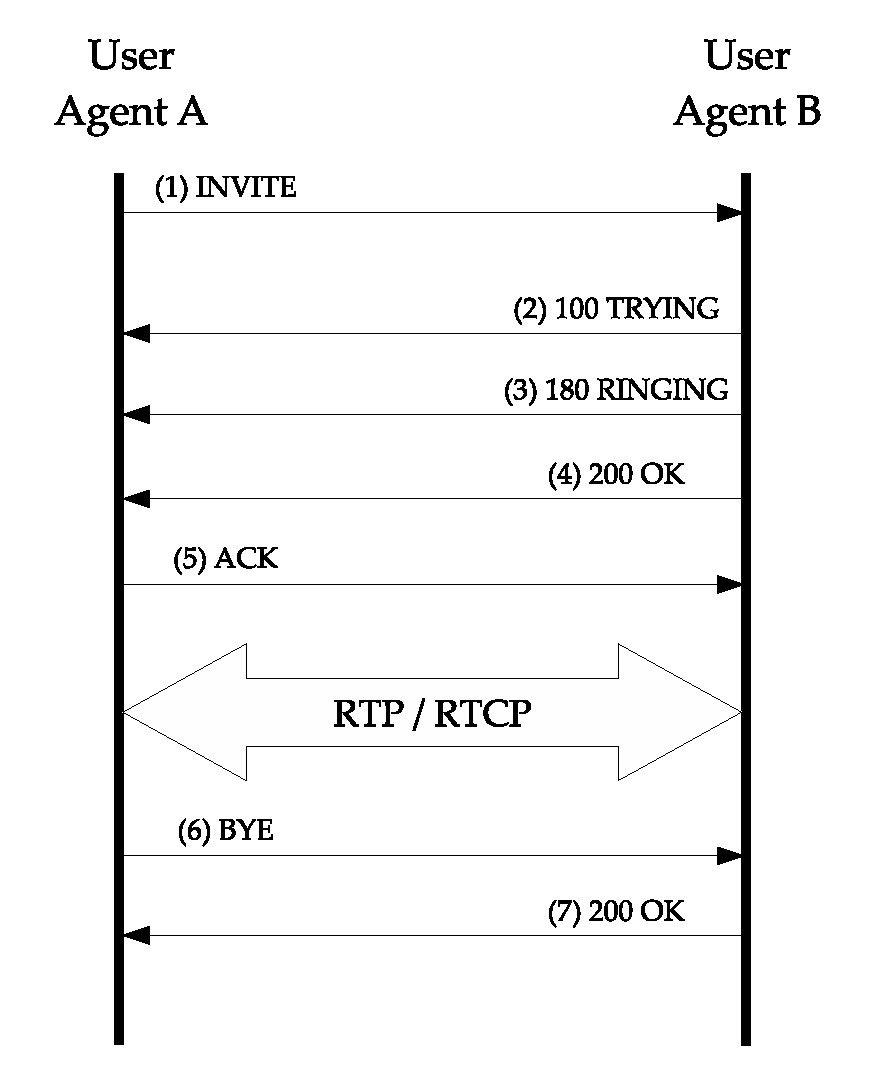
\includegraphics[width=.60\textwidth]{grafiken/sipanruf.eps}
	\caption{Sip Anruf ohne Proxy}
	\label{fig:sipanruf}
\end{figure}
\subsection{Registrierung der Lokation von Teilnehmern}

\begin{figure}[tbh]
	\centering
		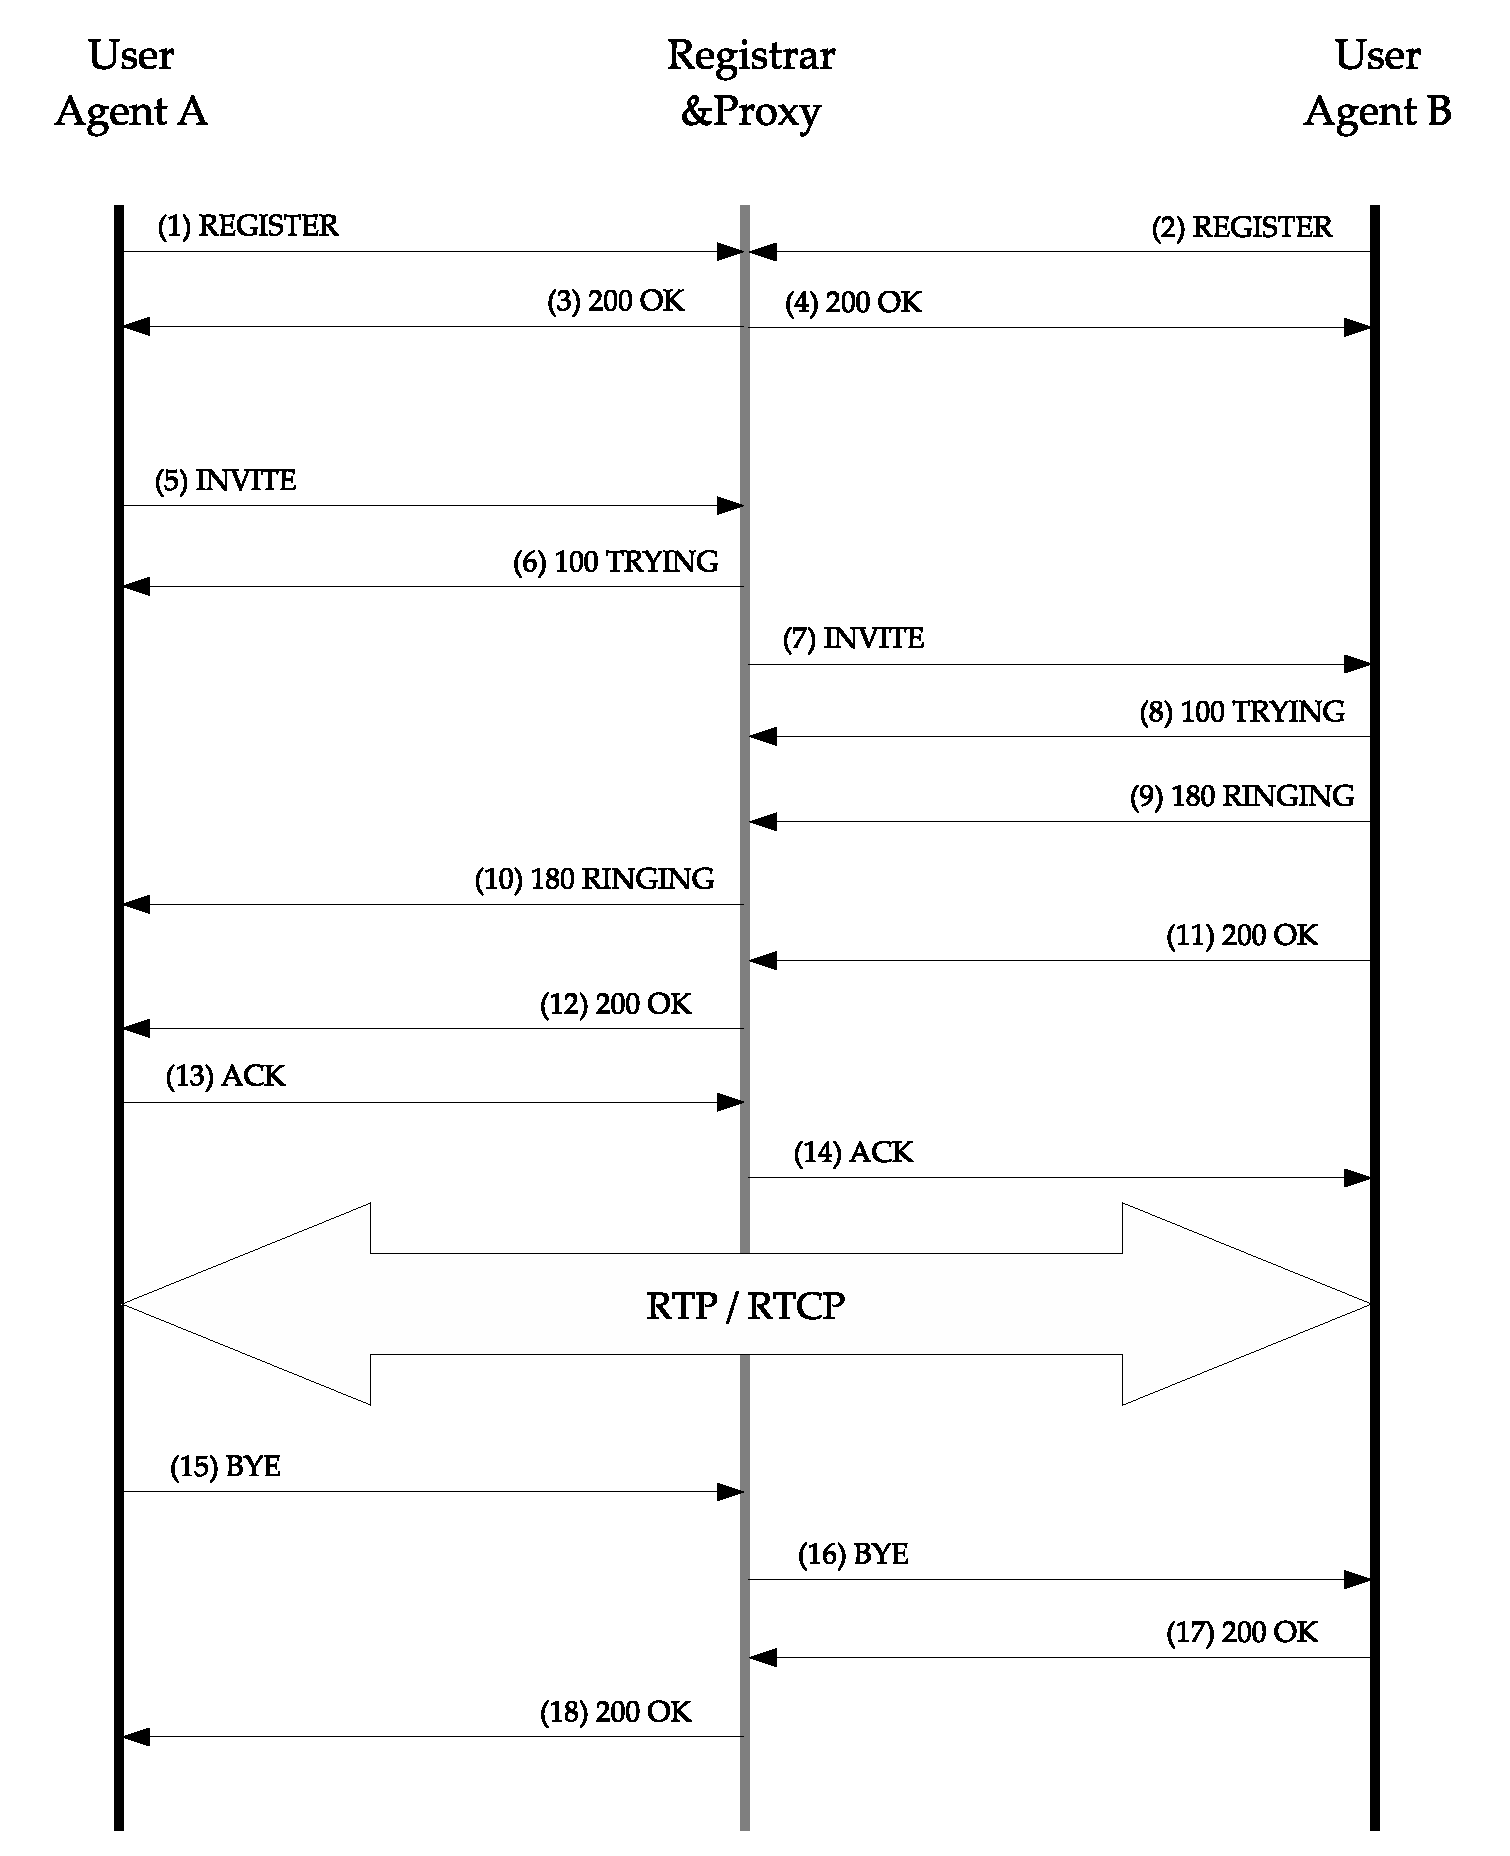
\includegraphics[width=1.00\textwidth]{grafiken/sipanrufmitproxy.eps}
	\caption{Einsatz eines Proxy Servers mit Registrar}
	\label{fig:sipanrufmitproxy}
\end{figure}

SIP definiert eine spezielle Komponente, die als Registrar bezeichnet wird. Ein Registrar enth�lt die Angaben hinsichtlich der Lokation von Teilnehmern in einer Domain. 

Dadurch, dass ein Teilnehmer mobil sein kann und verschiedene Clients benutzen kann, k�nnen ihm auch verschiedene Lokationen zugeordnet werden und so kann er seine aktuelle Lokation beim Registrar anmelden. Hierf�r wird die Request Nachricht REGISTER verwendet. Mit dieser Nachricht kann jeder Teilnehmer die Umleitung der bei ihm ankommenden Anrufe selbst veranlassen. 

M�chte ein Teilnehmer mit der SIP Adresse \textit{sip:bob@uni-mannheim.de} in seiner Heimat-Domain \textit{uni-mannheim.de} Anrufe entgegennehmen, so wird an den Registrar, z.B. \textit{registrar.uni-mannheim.de}, mit der Request Nachricht REGISTER, dieser Wunsch mitgeteilt. Relevante Felder der Nachricht enthalten die Herkunft (From), die Lokation des Benutzers(Contact) und die G�ltigkeit der Nachricht(Expires). Wechselt der Benutzer vor Ablauf der Expire Zeit seine Lokation, so wird der Registrar mit einer weiteren Nachricht dar�ber aktualisiert. Der Registrar best�tigt den Empfang der Nachrichten jeweils mit einer ACK Nachricht. Ebenso ist eine Registrierung �ber eine andere Person m�glich, so kann z.B. die Sekret�rin die aktuelle Lokation ihres Chefs aktualisieren. 

\subsection{Instant Messaging zwischen Teilnehmern}

Als Instant Messaging wird im allgemeinen ein Dienst zur sofortigen �bermittlung von Nachrichten zwischen Teilnehmern eines Netzwerks verstanden. Es existieren viele propriet�re Protokolle wie IRC(Internet Relay Chat), XMPP(Extensible Messaging and Presence Protocol) und OSCAR(Open System for CommunicAtion in Realtime). Auch bei SIP wurde in den RFCs 3860, 3428 und 3265 ein Protokoll f�r das Instant Messaging definiert: SIMPLE (SIP for Instant Messaging and Presence). 

Eine SIP MESSAGE Transaktion kann sowohl �ber einen PROXY laufen als auch direkt zwischen den UACs stattfinden. M�chte Teilnehmer A eine Nachricht an Teilnehmer B verschicken, so wird diese mittels der MESSAGE Nachricht versendet und vom Empf�nger mit einer ACK Nachricht best�tigt. Die wichtigsten Felder der MESSAGE Nachricht sind das Empf�nger Feld(To), der Typ des Inhalts(Content-Type), dessen L�nge(Content-Length) und der Inhalt selbst(Body). 

\begin{figure}
	\centering
		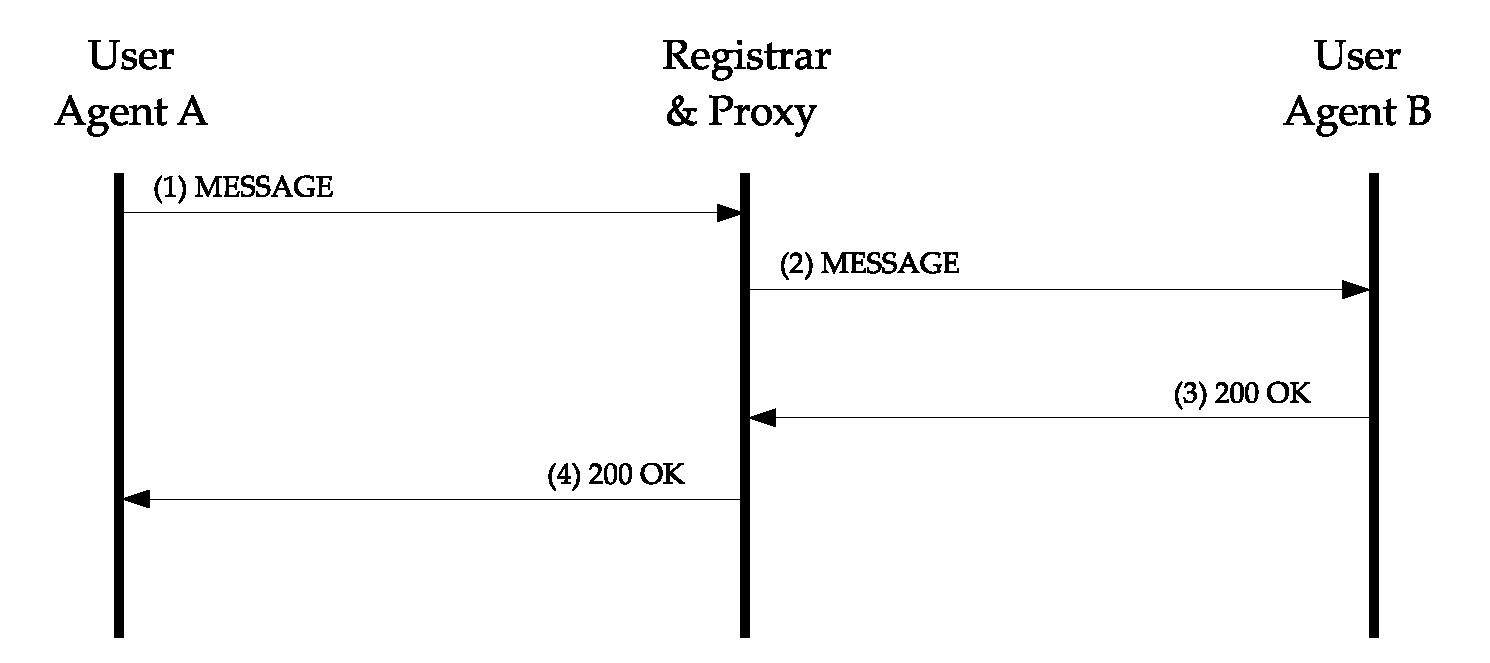
\includegraphics[width=1.00\textwidth]{grafiken/sipmessage.eps}
	\caption{Teilnehmer A schickt Teilnehmer B eine Nachricht. Beide sind Teil der gleichen Dom�ne und benutzen den gleichen Proxy.}
	\label{fig:sipmessage}
\end{figure}

Der Grundlegende Unterschied zum SIP Protokoll beruht darauf, dass hier kein separater Medienstrom existiert. Die Textnachrichten werden in einem SIP Paket �ber die Knoten �bertragen, die den Signalisierungspfad bilden. Dies erfordert ein gr��eres Bed�rfnis nach Sicherheit als bei anderen SIP Anfragen, da der Benutzer dem Proxy vertrauen muss. Unverschl�sselte Nachrichten liegen diesem offen und auch eventuelles Abzweigen von Nachrichten (\textit{Forking}) ohne Wissen des Benutzers ist hier m�glich. 

%RFC 3428
\subsection{Pr�senzfunktion von Teilnehmern}

% Grafik �ber Publish Subscribe

Die SIP Pr�senzfunktion dient zur Anzeige des Pr�senzstatus anderer Teilnehmer. Die Verwendung eines Pr�senzstatus ist in vielen Instant Messaging Anwendungen weit verbreitet und in verschiedenen Protokollen wie IMPS, XMPP etabliert. SIP besitzt eine eigene Erweiterung f�r Ereignisse, die in den RFCs 3265 und 3903 definiert wurde. Diese beinhaltet die Nachrichtentypen PUBLISH, SUBSCRIBE und NOTIFY. 

Will ein Teilnehmer ein Ereignis wie z.B. seine Status�nderung ver�ffentlichen, so schickt er eine PUBLISH Nachricht an den Presence-Server, der �blicherweise Teil eines Proxys ist. Dabei enth�lt die Nachricht den Event Typ im Header, die relevanten PUBLISH Informationen im XML Format im Body Feld. Grunds�tzlich sind beliebige Formate nutzbar, wobei ein Standard speziell f�r die Pr�senz\-information PIDF (Presence Information Data Format) existiert. Ein solches PIDF Tupel kann Beispielsweise den Namen des Teilnehmers, seinen Status und eine NTP Zeit enthalten. 

 Um z.B. die Pr�senz bestimmter Teilnehmer zu abonnieren versendet der Benutzer eine SUBSCRIBE Nachricht an den Presence-Server. Die L�nge des Dialogs wird durch das Laufzeit-Feld deklariert (Expires). Soll ein Abonne\-ment vorzeitig gek�ndigt werden, so eine SUBSCRIBE Nachricht mit der Laufzeit 0s verschickt werden. Der Erhalt einer solchen Nachricht f�hrt dazu, dass ein Dialog zwischen Presence Server und dem Teilnehmer eingeleitet wird. Eine NOTIFY Transaktion informiert nun den Abonnenten �ber seine abonnierten Ereignisse wie z.B. den Pr�senzstatus eines Teilnehmers. 

\begin{figure}[tbh]
	\centering
		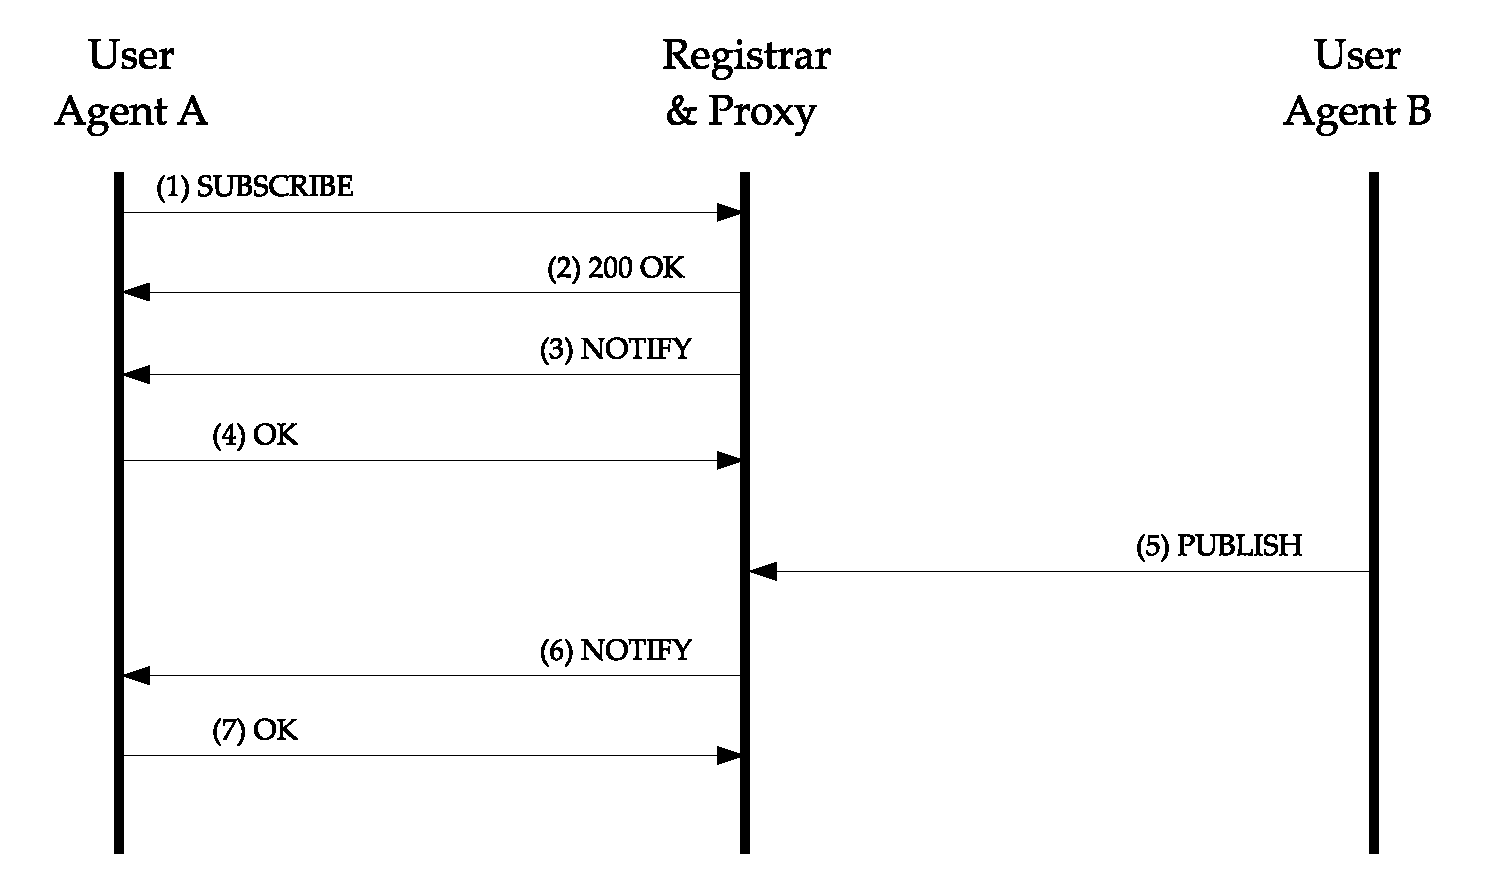
\includegraphics[width=1.00\textwidth]{grafiken/sippresence.eps}
	\caption{Teilnehmer A m�chte die Pr�senz von Teilnehmer B abonnieren. Teilnehmer B aktualisiert seine Information.}
	\label{fig:sippresence}
\end{figure}

\section{Session Description Protokoll}
Das Session Description Protokoll wird vom Signalisierungsprotokoll SIP dazu benutzt, die Eigenschaften des Medienstroms sowie den verwendeten Codec, Transportprotokoll und Zieladresse mit Port festzulegen. 

\subsection{Aufbau von SDP Nachrichten}
\label{sdp-aufbau}

SDP ist ein textbasiertes Format, in dem die Eigenschaft und der Wert in Textform in der Nachricht festgehalten werden. Die Nachricht enth�lt die Besonderheiten der RTP-Session, die durch das SDP Protokoll festgelegt wird. Die Nachricht setzt sich aus der Spezifikation der RTP-Session, der Zeitbeschreibung und der Medienbeschreibung zusammen. 

% Bild der SDP message
% Bild vom SIP Message
\begin{figure}
\lstset{frame=single}
	\begin{lstlisting}[label={SIP-Message}]
v=0
o=Anonymous 1234567890 1234567890 IN IP4 192.168.3.250
s=Testing the SDP Message
t=0 0
m=audio 6006 RTP/AVP 8 3 0
a=rtpmap:8 PCMA/8000
a=rtpmap:3 GSM/8000
a=rtpmap:0 PCMU/8000
\end{lstlisting}
\caption{Beispiel einer SDP Nachricht}
\end{figure}


Die Beschreibung der RTP-Session wird mit den folgenden Parametern definiert:
\begin{itemize}
	\item v: Gibt die verwendete RTP Version an.
	\item o: Enth�lt den Initiator der Nachricht an:
	\subitem $\left\langle username \right\rangle$: den Namen des Initiators der Session
	\subitem $\left\langle session id \right\rangle$: die Identifikation der Session, meistens der NTP-Stempel.
	\subitem $\left\langle network type \right\rangle$: der Netztyp
	\subitem $\left\langle address type \right\rangle$: der Typ der Quell-IP-Adresse
	\subitem $\left\langle adress \right\rangle$: die Quell-IP-Adresse
	\item s: Gibt eine genauere Bezeichnung der Session an z.B. den Namen
	\item t: Bestimmt die Start und Endzeit der Session. 
	\item m: In der Media Zeile werden folgende Parameter angegeben:
	\subitem $\left\langle media \right\rangle$: Hier wird die Medienart (z.B. Audio) definiert.
	\subitem $\left\langle port \right\rangle$: Die Portnummer �ber den das Medium empfangen wird.
	\subitem $\left\langle transport \right\rangle$: Das verwendete Transportprotokoll
	\subitem $\left\langle fmt list \right\rangle$: Eine Liste der zul�ssigen Formate des Mediums. 
	\item a: Hier wird eine Liste angegeben welches Format des Mediums empfangen werden kann. 
\end{itemize}

Den "`klassischen"' Audio Formaten sind feste Nummern\footnote{Eine �bersicht �blicher PT-Nummern ist in der Tabelle \ref{pt-tabelle} dargestellt} zugeordnet. Weitere Typen befinden sich im dynamischen Bereich und k�nnen f�r jede Sitzung zu beliebigen Medienformaten vereinbart werden.

\subsection{Aushandeln der Sitzungsparameter}
Die unter dem Parameter \textbf{"`a"'} ausgetauschte Liste der Medienformate entspricht in der Reihenfolge der Pr�ferenzen des Senders. Der Empf�nger eines solchen Angebots beantwortet jedes empfangene Medienformat mit einer Korrespondierenden Antwort, falls er dieses Medienformat unterst�tzt. Ein Medienstrom kann vom Empf�nger abgelehnt werden, wenn keines der aufgelisteten Medienformate unterst�tzt wird, indem als Port eine Null gesendet wird. Nach M�glichkeit sollte die Reihenfolge die unterst�tzten Medienformate aus dem Angebot beibehalten und nicht unterst�tzte Formate sollten ausgeblendet werden.

Nachdem sich beide Teilnehmer auf die unterst�tzten Formate geeinigt haben, k�nnen beide Seiten damit beginnen, die Mediendaten zu senden. Beide Seiten sollten jeweils das bevorzugte Format senden. W�hrend einer Sitzung k�nnen die Parameter neu verhandelt werden, indem der gleiche Ablauf mit entsprechend modifizierten SDP-Beschreibungen durchgef�hrt wird. 

\section{Real-Time Transport Protokoll}
Speziell f�r die �bermittlung von Sprache, Audio und Video �ber IP-Netze wurde RTP (Real-time Transport Protocol) bei der IETF entwickelt (RFC 2550). Einerseits stellt RTP ein Transportprotokoll f�r die Echtzeitmedien dar, anderseits kann es als eine Anwendungsart oberhalb des verbindungslosen Protokolls UDP angesehen werden. 

Die Wichtigsten Besonderheiten von RTP sind:

\begin{itemize}
	\item �bermittlung von Echtzeitmedien in RTP-Paketen: Echtzeitmedien werden in RTP als eine zusammenh�ngende Folge von RTP-Paketen �ber eine RTP-Session �bermittelt. 
	\item Garantie der Reihenfolge von RTP-Paketen: RTP nummeriert die �ber\-tra\-genen Pakete mit Echtzeit\-medien, sodass ihre richtige Reihenfolge am Ziel wiederhergestellt werden kann, falls sie durch den Transport �ber das IP-Netz ver�ndert wurde. 
	\item Garantie der Synchronit�t: RTP vergibt den �bertragenen Paketen einen Zeitstempel, sodass die gleichen Zeitabst�nde am Ziel wiederhergestellt werden k�nnen, die beim Absender bestanden. 
	\item Transport unterschiedlicher Formate: Es k�nnen unterschiedliche Formate wie Audio, Sprache und Video �bertragen werden, die in unterschiedlichen Profiles genau bezeichnet werden. 
\end{itemize}

\subsection{Aufbau von RTP-Paketen}
RTP �bermittelt ein Echtzeitmedium als Folge von RTP Paketen, die mit einem vorangestellten UDP-Header in den IP-Paketen transportiert werden. Jedes RTP-Paket enth�lt einen RTP-Header und die Nutzlast(\textit{Payload}). Die wesentlichen Angaben im RTP-Header sind:

\begin{figure}
	\centering
		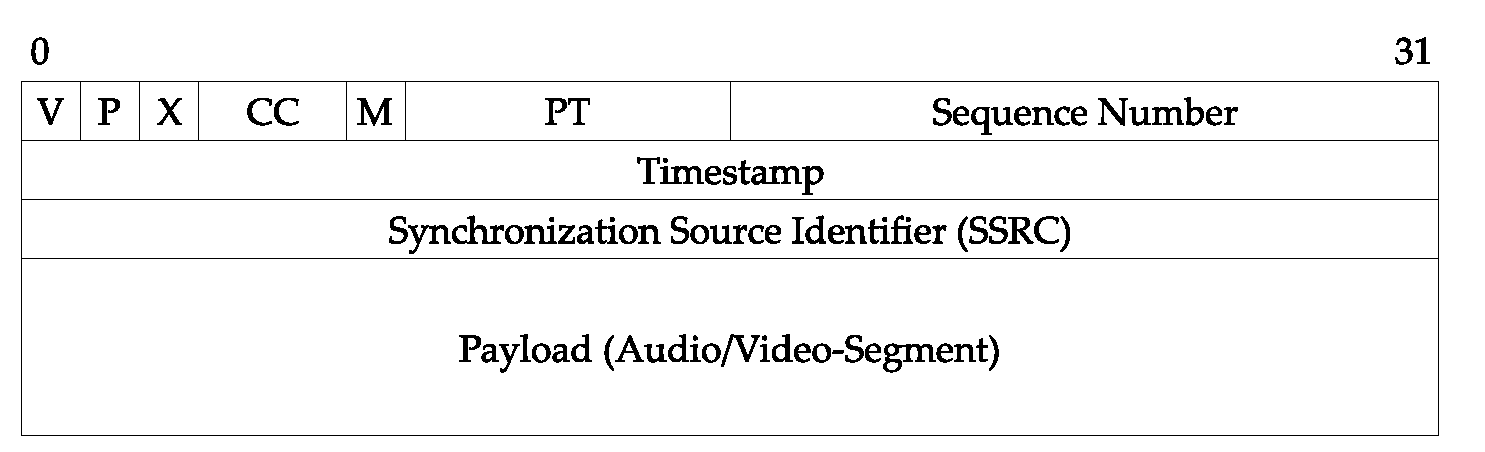
\includegraphics[width=1.00\textwidth]{grafiken/rtppaket.eps}
	\caption{Header eines RTP-Pakets}
	\label{fig:rtppaket}
\end{figure}

\begin{itemize}
	\item PT (\textit{Payload Type}): Es wird angegeben, um welches Format es sich beim transportierten Medium handelt, dh. nach welchem Verfahren codiert wurde. Die M�glichen Kodierungsarten sind in RFC 3551 festgelegt. 
	\item Timestamp: Der Zeitstempel dient dazu, den Zeitpunkt der Generierung vom \textit{Payload} zu markieren. Der Zeitstempel ist n�tig, um die Schwankungen der �bertragungszeit (Jitter) von RTP-Paketen beim Empf�nger auszugleichen. 
	\item Sequence Number: Jedes RTP-Paket wird mit einer Sequenznummer versehen, die es dem Empf�nger erlaubt, den Verlust von Paketen festzustellen, bzw. die Reihenfolge wiederherzustellen, falls sie in einer falschen Reihenfolge angekommen sind. 
	\item SSRC (\textit{Synchronization Source Identifier}): Zur Identifikation der Quelle(Mikrofon, Kamera) dient der SSRC. Zwei verschiedene Quellen m�ssen unterschiedliche SSRCs haben, um f�r den Empf�nger unterscheidbar zu sein. 
	\item CSRC(\textit{Contributing Source Identifier}): Wird optional verwendet und enth�lt die "`Orginal"'-Quellen der Bitstr�me falls der SSRC von einem Mixer ver�ndert wurde.
\end{itemize}

Die PT Nummern dienen zur Identifikation der einzelnen Audio- und Video-Formate. Da der Nummernraum nicht komplett belegt ist, k�nnen weitere Nummern vergeben werden (dynamische PT-Nummern). Bei der Verwendung von dynamischen PT-Nummern wird die Kompatibilit�t zwischen Empf�nger und Sender mit Hilfe des SDP Protokolls vereinbart (siehe Tabelle \ref{pt-tabelle}).

\subsection{RTP Control Protokoll}
RTP wird mit RTCP so erg�nzt, dass Information �ber den Verlauf der Kommunikation zwischen Sender und Empf�nger, insbesondere �ber die Qualit�t der �bertragung, ausgetauscht werden k�nnen. 

Die wichtigsten Aufgaben von RTCP sind die �berwachung der �ber\-tragungs\-qualit�t: Hierf�r werden zwischen Sender und Empf�nger laufend Informationen �ber die Qualit�t der �bertragung mittels Sender- und Receiverreports ausgetauscht. Dies Erm�glicht es dem Sender, den von ihm generierten Bitstrom an die Netzbedingungen anzupassen und so Fehler einzugrenzen. 

\subsubsection{Typen und Struktur der RTCP-Pakete}
Beim RTCP werden folgende RTCP-Pakete als Nachrichten verwendet. 
\begin{itemize}
	\item Sender Report (SR)
	\item Receiver Report(RR)
	\item Source Description (SDES)
	\item Abmeldung (BYE)
	\item Applikationsspezifisches Paket (APP)
\end{itemize}

RTCP Pakete beginnen mit einem Header und k�nnen unabh�ngig von anderen bearbeitet werden. Die Reihenfolge der Pakete in einem IP-Paket kann beliebig sein. 
Das SR Paket enth�lt einen Zeitstempel gem�� der NTP (Network Time Prococol) und beschreibt die Qualit�t der �bermittlung aus Sicht des Senders. So kann z.B. dem Empf�nger die Sendedatenrate mitgeteilt werden, damit dieser sich im Voraus auf die ankommende Datenmenge einstellen kann. 

In einem Sender Report sind immer enthalten:
\begin{itemize}
	\item NTP-Zeitstempel: Ein Zeitstempel gem�� der NTP Uhrzeit. 
	\item RTP-Zeitstempel: Die NTP-Zeit in Zeiteinheiten der RTP Session, die pri\-m�r dazu dient um verschiedene Quellen zu synchronisieren.
	\item Gesendete Pakete: Die Anzahl der gesendeten Pakete sowie Bytes.
\end{itemize}

Beim RR Paket werden Werte wie Jitter, Round-Trip-Delay (Hin und Zur�ck Verz�gerung)  oder Paketverlust aus Sicht des Empf�ngers berechnet und abgesch�tzt. 

In einem Receiver Report sind unter anderem folgende Informationen enthalten:
\begin{enumerate}
	\item Paketverlust: Der Anteil der verlorenen Pakete seit dem letzten Report, als auch die Gesamtanzahl der verlorenen Pakete.
	\item Jitter: Der Jitter wird gesch�tzt als die Varianz der Ankunftszeitdifferenzen der Pakete. 
	\item Letzter Report: Die verstrichene Zeit seit dem Empfang des letzten Reports.
\end{enumerate}

Die SDES Pakete erm�glichen es, die Quellen mit Namen zu kennzeichnen. Diese Kennzeichnung wird vom Empf�nger dazu verwendet, mehrere Bitstr�me einer Quelle, die in getrennten RTP-Sessions �bertragen werden, wieder zusammenzuf�hren. Das BYE Paket dient dazu das Ende der Teilnahme an einer Kommunikation anzuzeigen. 

\subsection{Silence Supression}
Teilnehmer einer Audio Verbindung m�ssen nicht unbedingt Audiopakete �ber den RTP Strom senden, falls gerade bei den Teilnehmern Stille herrscht. Diese Funktion wurde im RFC 3389 spezifiziert.

Die M�glichkeit, den RTP Paketversand w�hrend Stilleperioden zu unterbrechen wird als Stille Unterdr�ckung (\textit{Silence Suppression}) oder Stimm-Aktivit�ts-Erkennung(\textit{Voice Activity Detection}) bezeichnet. Silcence Suppression kann vom Empf�nger erkannt werden, wenn der RTP Zeitstempel nicht mit dem Intervall �bereinstimmt, das vom letzten Paket abgedeckt wurde, obwohl die RTP Sequenznummer sich nur um 1 erh�ht hat. Ob Silence Suppression eingesetzt wird, h�ngt normalerweise von der Konfiguration der beiden Endpunkte ab.

\section{NAT Traversal} 
Unter NAT Traversal versteht man das Erkennen und Durchdringen von Firewalls und NAT-Routern. Hier gibt es mehrere Ans�tze wie TURN (Traversal Using Relay NAT) \cite{turn08}, ICE (Interactive Connectivity Establishment) \cite{ice08} und STUN (Simple Traversal of User Datagram Protocol Through Network Adress Translators) \cite{stun03}. 
%Diese Protokolle helfen vor allem Peer-to-Peer Protokollfamilien, die durch NATs in ihrer Funktionsweise behindert werden. Beispiele solcher Protokolle sind generell alle Peer-to-Peer Protokolle die Multimediakommunikation, Datenaustausch oder Spielen erm�glichen. 

Unter STUN versteht man ein einfaches Protokoll, das es erlaubt Anwendungen festzustellen, ob sie sich hinter einer Firewall oder einem Router mit NAT (Network Adress Translator) befinden und um welche Kategorie von Router es sich handelt. Ebenso ist es mit STUN m�glich seine �ffentliche IP Adresse herauszufinden. 

Die typische STUN Konfiguration beinhaltet einen STUN Client, der in einem privaten Netzwerk beheimatet ist. Dieses Netzwerk wird mit dem Internet durch einen NAT verbunden. Ein weiteres privates Netzwerk das ebenfalls durch einen NAT verbunden ist, beheimatet einen weiteren STUN Client. Der STUN Server befindet sich im �ffentlichen Internet. M�chte nun eine Client- Anwendung seine �ffentliche IP Adresse und Port erfahren auf der sie Daten empfangen kann, sendet der STUN Client in der Anwendung einen STUN "`\textit{Shared Secret Request}"' an den STUN Server und dann einen \textit{Binding Request}. Daf�r muss dem Client mindestens die Adresse eines �ffentlichen STUN Servers bekannt sein. Ein \textit{Binding Request} wird benutzt, um die Anwesenheit eines NATs festzustellen und um die �ffentliche IP Adresse und Port zu erfahren, die der NAT generiert hat. Vom STUN Server wird ein solcher Request mit einer \textit{Binding Response} beantwortet, die genau diese Daten zur�ck an den Client schickt. Erh�lt nun ein STUN-Client eine \textit{Binding Response}, vergleicht er die IP-Adresse und den Port mit seiner lokalen IP Adresse und Sendereport und kann so feststellen, ob es sich hinter einem NAT befindet. Nachdem beide Clients ihre �ffentlichen IP-Adressen und Port Paare kennen, sind sie in der Lage direkt miteinander zu kommunizieren. 

\begin{figure}[tbh]
	\centering
		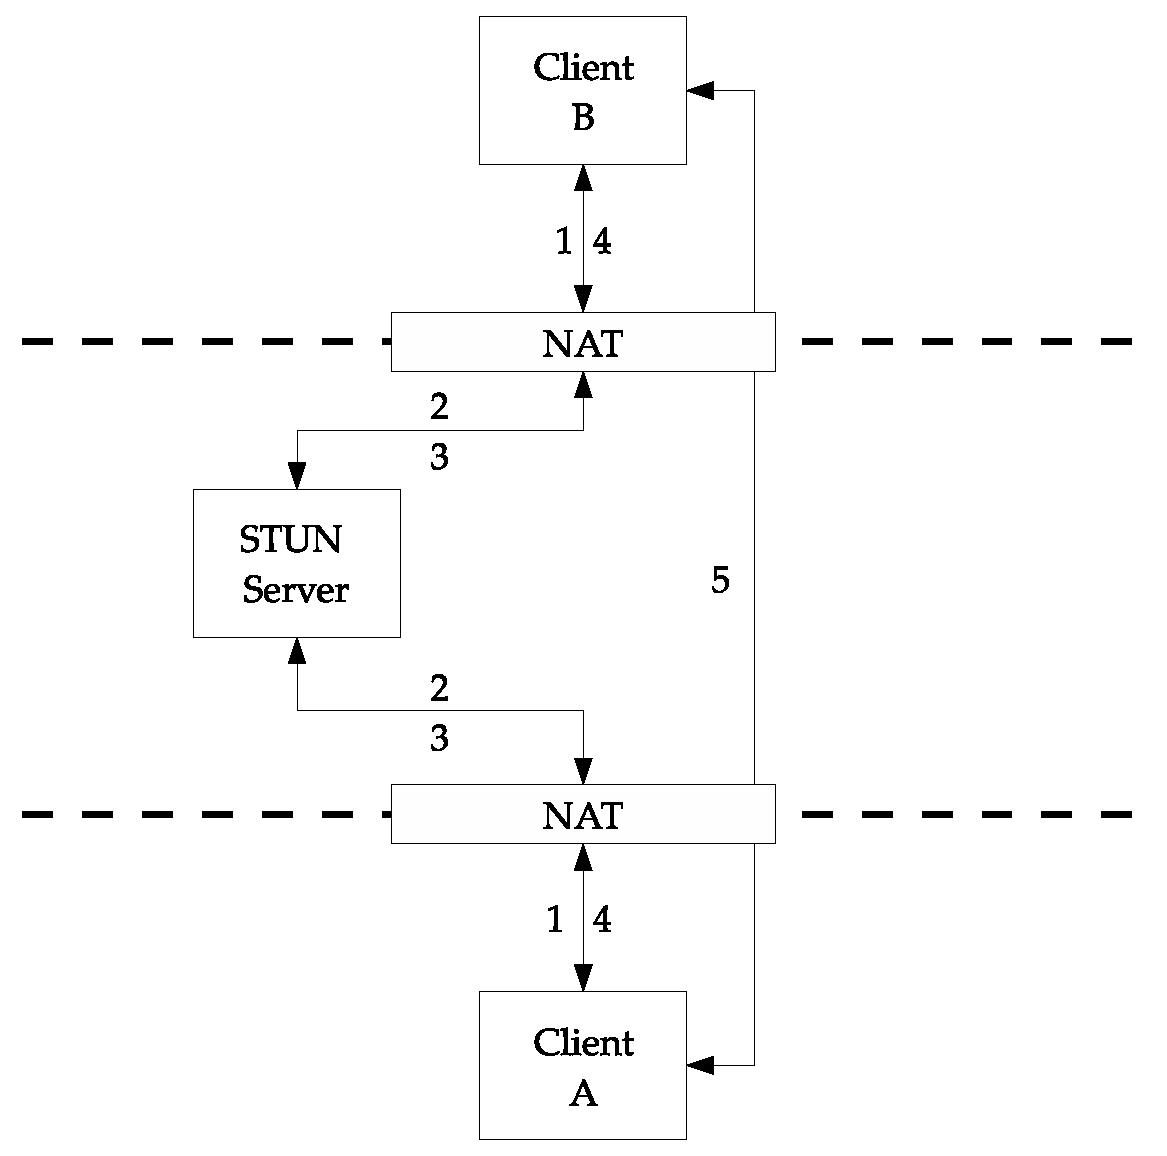
\includegraphics[width=0.60\textwidth]{grafiken/stun.eps}
	\caption{Ein schematischer Ablauf von STUN}
	\label{fig:stun}
\end{figure}

%Grafik von STUN Transaktion

%\section{Skype}
%\subsection{Registrierung und Login}
%\subsection{Rufsignalisierung und Sprach�bertragung}
%\subsection{Technologie von Skype}
%\subsubsection{Verbindungsstruktur}
%\subsubsection{Sicherheit}
%\subsubsection{Konferenzen}



\newpage~
\chapter{Verwandte Arbeiten}

Dieses Kapitel liefert eine �bersicht �ber bisherige akademische Ans�tze eine Sprachkommunikation in Computerspielen umzusetzen. Die vorgestellten Konzepte unterscheiden sich Haupts�chlich darin, ob die Signalisierung und das Abmischen des Audiosignals serverbasiert oder dezentralisiert stattfindet. 

\section{Historische Ans�tze}
Erste Arbeiten, die sich mit Audio in Mehrspieler-Computerspielen auseinandersetzen, haben ihren Ursprung in den SPLINE \cite{carlsson93} und DIVER \cite{anderson95} Systemen. Diese sahen vor, dass sich Clients mit einem zentralen Server verbinden, um Spielerpositionen auszutauschen. Spieler erhalten zwar eine lokalisierte Audioszene entsprechend ihrer Position, k�nnen jedoch keine Sprachkommunikation untereinander aufbauen. 

Erste Ans�tze f�r eine Sprachkommunikation in Computerspielen finden sich im MiMaze-Spiel \cite{diot99}. Mimaze war entwickelt worden, um �bertragungs- und Kontrollmechanismen in Internet-Spielen zu erforschen. Der Ansatz sah vor, dass der Datenaustausch zwischen Spielern und Server mittels TCP stattfindet und zwischen den Spielern untereinander mittels UDP Multicast Gruppen etabliert werden. Dabei wurde die Spielewelt auf dem Server verwaltet und jegliche Aktionen im Spiel mit UDP Multicast Gruppen zwischen den Spielern ausgetauscht. Bolot und Fosse-Parisis versuchten in \cite{bolot98}, die bestehende Architektur des MiMaze Spiels um die Sprachkommunikation zu erweitern. Dazu schlugen sie vor, das RTP und RTCP-Protokoll einzusetzen und die empfangenen Audiostr�me auf den Clients zu lokalisieren. Aufgrund der schwierigen Koordination der Audiostr�me und deren Synchronisation mit der Spielewelt blieb der Einsatz von Sprachkommunikation in Computerspielen zun�chst ein Entwurf. 

\section{Serverbasierte Ans�tze}

\subsection{DICE: Internet Delivery of Immersive Voice Communi\-cation for Crowded Virtual Spaces}

Im DICE System \cite{safei05} schlagen Safei und Boustead einen Entwurf einer serverbasierten Architektur f�r die Sprachkommunikation f�r Mehrspieler Spiele im Internet vor. Dieses System beruht auf dem Prinzip, dass eine zentrale Komponente f�r die Verteilung von Audiostr�men verantwortlich ist, deren Abmischen jedoch lokal auf den Clients geschieht. Dabei soll jeder Spieler eine Mischung aus Stimmen und Ger�uschen h�ren, die speziell auf seine Position im Spiel angepasst ist. Es soll sowohl die Lautst�rke als auch die Position der Stimmen in der Audioszene abgebildet werden. Die Architektur baut auf einem verteilten Server-System auf, da vorhergehende Studien \cite{safei04} von Safei gezeigt hatten, dass eine einzige Serverkomponente die Delay Anforderungen nicht erf�llen kann. 

Die Elemente des Systems bestehen aus einem Audio-Client, der seinen Mono-Audiostrom an den Scene Creation Server schickt und alle bestehenden Audiostr�me von ihm empf�ngt. Der Audio-Client ist anhand der Positionen der Avatare im Spiel in der Lage, die empfangenen Audiostr�me r�umlich zu positionieren. 

Auf dem Scene Creation Server wird das r�umliche Umfeld jedes Spielers in Cluster eingeteilt, die nur Spieler beinhalten, deren Entfernung und Winkel zum Spieler �hnlich sind. Spieler, die sich im gleichen Cluster befinden, werden von diesem in einen Audiostrom zusammengemischt und an den entsprechenden Audio-Client inklusive der Positionsinformationen dieses Clusters weitergeleitet. Diese Methode soll daf�r sorgen, dass nicht alle Audiostr�me separat an den Audio-Client gesendet werden m�ssen und eventuell sogar schon auf dem Server gemischt werden k�nnen, um so Bandbreite einzusparen. Dabei wird ein maximaler Distanz- und Winkelfehler zugelassen, der zwar die Qualit�t der exakten Positionierung vermindert, es aber erlaubt mehrere Spieler in das gleiche Cluster zu mischen.

Der Scene Creation Server wird dabei vom darunter liegenden Control-Server verwaltet, der dar�ber entscheidet, welche Audiostr�me an den Audio-Client geschickt werden sollen, damit dieser in der Lage ist die Audioszene zu erzeugen. 

\subsection{MICE: Mobile Immersice Communication Environment}

Das MICE System \cite{safei06b} von Safei und Boustead ist der Entwurf einer serverbasierten Sprachkommunikation f�r Mehrspieler-Spiele, die auf mobilen Endger�ten zum Einsatz kommen. Die spezielle Herausforderung besteht darin, dass solche Ger�te �ber eine geringe Bandbreite und Rechenleistung verf�gen. Dabei �hnelt der Ansatz dem DICE System, da auch jeder Spieler seine Monoquelle an den Server sendet. Der Unterschied zum DICE System besteht darin, dass die Erzeugung der Audioszene komplett auf dem Server geschieht und nur das fertige Resultat als Stereo-Audiostrom an den Client �bertragen wird. 

Dazu wird mittels HRTF (Head Related Transfer Function) \cite{bergault94}, einer Technik, die es erlaubt Kl�nge im dreidimensionalen Raum zu positionieren, eine Audioszene erzeugt. Jeweils zwei verschiedene Signale werden f�r das rechte und linke Ohr erzeugt, aus deren Unterschied das menschliche Ohr die Quelle im Raum positionieren kann. F�r die Berechnung der HRTF-Funktion ben�tigt man die Richtungsvektoren aller Quellen. 

�hnlich wie im DICE-Ansatz schlagen Safei und Boustead vor, ein Clustering vorzunehmen und f�r Spieler mit �hnlicher Position und �hnlichem Richtungsvektor einen Gesamtrichtungsvektor zu benutzen. Dadurch entsteht auch wie beim DICE System ein Distanz- und Winkelfehler, der jedoch mit Hilfe eines linearen Optimierungsproblems unter einen experimentell festgelegten Schwellwert minimiert wird. Dieser Schwellwert wird f�r nahe Audioquellen niedriger gesetzt, als f�r Quellen die weit entfernt sind, da Untersuchungen gezeigt haben, dass in Abh�ngigkeit von der Entfernung ein unterschiedlich gro�er Fehler von Probanden akzeptiert wird \cite{safei06}, \cite{safei07}. 

%Dazu wurden die Erfahrungen von 27 Probanden Anhand des Standardisierten Mean Opition Score \cite{mtu96} analysiert und es wurde festgestellt, dass Unterschiede bis zu 35 $\circ$ Grad akzeptiert werden. In einer weiteren Studie schlagen Safaei und Downlatshahi vor die zentralisierte Server Architektur durch eine Anzahl an lokalen Proxies zu ersetzen, die selbst in einem Multicast Overlay verbunden sind \cite{safaei06}. 

\subsection{Session Initiation Protocol for Multiplayer Networked Games}

Singh und Acharya schlagen ein auf dem Session Initiation Protocoll basiertes System vor, um VoIP in Mehrspieler-Spielen zu realisieren \cite{singh04}. Dazu f�hren sie einen Konferenz-Server ein, der eng mit dem Spieleserver zusammen arbeitet. Der Konferenz-Server kontrolliert und initiiert die Sitzungen f�r alle Spielteilnehmer und verwaltet ebenfalls die Mixerkomponente des Systems. Diese ist f�r das dedizierte Mischen der verschiedenen Audiostr�me zust�ndig. Dabei wird die Konferenz zwischen den Clients und dem Konferenz-Server initiiert, der Datenstrom selbst jedoch flie�t zwischen dem Mixer und den Clients. 

In einem zentralisierten Ansatz veranlasst die Spielelogik auf dem Spieleserver Spieler Konferenzen in Abh�ngigkeit ihrer Position auf dem Spielfeld betreten. Das Spielfeld wird in mehrere Zonen aufgeteilt, f�r die im Konferenz-Server Konferenzen reserviert werden.
 
In einem dezentralisierten Ansatz enthalten die Clients die Spielelogik, die sie veranlasst entsprechend mit dem Konferenz-Server Konferenzen zu initiieren. 

Beide F�lle unterscheiden zwischen einem statischen und dynamischen Ansatz. Der statische Ansatz sieht eine Konferenz f�r jedes Team vor, die vom ersten Teilnehmer der Konferenz initiiert wird und w�hrend der gesamten Spielzeit aufrechterhalten wird. 

Die Teilnahme an einer Konferenz auf dem Konferenz-Server h�ngt beim dynamische Ansatz von der Position der Spieler auf dem Spielfeld vor. So k�nnen f�r verschiedene R�ume oder Orte verschiedene Konferenzen existieren. Dabei findet der �bergang von einer Konferenz zur anderen f�r den Spieler selbst nahtlos statt, da sich die Signalisierung nur zwischen Gameserver und Konferenz-Server bzw. Mixer abspielt. 

In weiterf�hrenden Studien \cite{singh05}, \cite{singh06} diskutieren Singh und Archaya eine Erweiterung des SIP-Ansatzes f�r interpersonelle Konferenzen. Sie schlagen vor, ihr bestehendes System so zu erweitern, dass jeder Spieler seine eigene Konferenz auf dem Server besitzt, die speziell nur f�r ihn alle Stimmen in seiner H�rn�he enth�lt und eine weitere Konferenz, die nur seine Stimme f�r andere Spieler enth�lt.

Wichtig hierbei ist, dass der Spieler zwar sein Audiosignal an die zweite Konferenz sendet, diese aber nicht h�ren will, da sie f�r die Mitspieler bestimmt ist. Das gew�nschte Verhalten f�r die zweite Konferenz �hnelt somit einer Ein-Weg-Konferenz.
Da SDP jedoch keine Ein-Weg-Konferenzen erlaubt, w�re erst in einem erweiterten SIP-Standard dieses Szenario vorstellbar. 

Eine weitere theoretische Erweiterung sieht vor, dass die Lautst�rke des Audio\-stroms von Spielern in der H�rn�he in Abh�ngigkeit von ihrer Distanz variiert werden soll, wobei  ein ungel�stes Probleme bei diesem Ansatz die Komponente des Mixers bleibt. Dieser m�sste um die M�glichkeit erweitert werden, Distanzvektoren in den Mischvorgang einzubeziehen. 

%\subsection{SIP und SOAP basiertes Konferenzframework}
%In einem anderen zentralisierten Ansatz \cite{schulzrinne02} schlagen Schukzrinne und Koskelainen ein Framework zur Kontrolle von Konferenzen vor das auf den SIP und SOAP( Simple Object Access Protocol) Standards basiert. W�hrend SOAP f�r die Kontrolle der Konferenzen verwendet wird findet der Aufbau der einzelnen Sitzungen im SIP Protokoll statt. 

\section{Dezentralisierte Ans�tze}

\subsection{Full-Mesh}

In \cite{schulzrinne03}, \cite{schulzrinne99} schlagen Schulzrinne et. Al ein verteiltes dezentralisiertes System vor, in dem alle Teilnehmer ein komplett verbundenes Netz (engl. full-mesh) bilden. Hier ist jeder Teilnehmer mit jedem anderen Teilnehmer verbunden. Dazu �bertr�gt jeder Teilnehmer seinen Audiostrom an alle anderen Teilnehmer, die dann lokal das Abmischen vornehmen. Um den Ansatz zu testen, simulieren sie ein solches Netz in verschiedenen Szenarien, in denen Teilnehmer  Konferenzen betreten, verlassen oder andere Teilnehmer zu Konferenzen einladen. Die Teilnehmer selbst haben keinerlei Information �ber die Topologie des Netzes und  k�nnen so nur durch das rekursive Einladen von Teilnehmern ein komplettes Netz bilden. Das Hauptproblem dabei ist, es exisitert dadurch eine eine Vielzahl an Ereignism�glichkeiten, die eintreten k�nnen. Schulzrinne et Al. zeigen, dass schon bei vier Teilnehmern, die einladen, das Spiel verlassen oder betreten bereits �ber 50 M�glichkeiten aus den genannten Permutationen m�glich sind. 


\subsection{Distributed Partial Mixing}

Radenkovic, Grennhalgh und Benford diskutieren  in \cite{radenkovic02} den Einsatz 
eines DPM (Distributed Partial Mixing), das auf Basis des RTP und RTCP-Protokolls und Multicast Gruppen funktioniert. Hier werden mehrere dedizierte Mixer eingesetzt, die nur solche Audiostr�me abmischen, die tats�chlich auch vom Teilnehmer benutzt werden. Dies soll einerseits erm�glichen, eine Vielzahl an Audiostr�men zu verwalten und andererseits die �berlastung des Netzwerks verhindern. 

Der Ansatz sieht vor, dass die dedizierten Mixer zun�chst die Audiostr�me der Clients entgegennehmen. Die Mixer selbst sind alle miteinander in einer Baumstruktur verbunden und in der Lage Audiostr�me untereinander weiterzuleiten. Je nach Konnektivit�t und Bandbreite der Mixer untereinander entscheiden diese, ob ein Zusammenmischen der Audiostr�me notwendig ist, oder alle Audiostr�me ungemischt weitergeleitet werden k�nnen. Da der Ansatz auf Multicast Gruppen basiert, ist er zwar in LANs umsetzbar, im Internet jedoch aufgrund der fehlenden Multicast-Unterst�tzung nicht realisierbar. 

\subsection{Verteiltes Mischen}

Gu, Yu und Shae schlagen ein dezentrales System vor \cite{gu05}, in dem sie die Verteilung des Audiostroms in zwei Phasen der Aggregation und Distribution aufteilen. Dabei verstehen sie unter Aggregation das Zusammenmischen der Audiostr�me und unter Distribution die Verteilung der gemischten Audiostr�me auf die einzelnen Clients. 
Dazu nimmt ein initialer Mischknoten, der eine gute Anbindung besitzt und m�glichst optimale Wege zu allen Teilnehmern hat zun�chst das Abmischen vor. Falls er jedoch �berlastet ist, kann er zus�tzliche Mischknoten ernennen, die seine Arbeit �bernehmen. Dabei k�nnen Mischknoten, falls sie unterlastet sind, ihre Aufgabe an den Vaterknoten wieder abgeben. Der Vorteil der Methode ist, es muss kein dedizierter Mischserver benutzt werden da theoretisch jeder Knoten diese Aufgabe �bernehmen kann. 

Der Hauptnachteil dieser Methode ist, dass jederzeit alle Knoten �ber die Topologie des Netzes informiert sein m�ssen und jederzeit den optimalen Mischknoten der Multicast-Gruppe kennen m�ssen. Die Distribution des Audiostroms und die Kontrolle der Clients dar�ber, welche Audiostr�me gemischt werden sollen wird nicht gel�st. 
%TODO

\subsection{SIP Konferenz Extension}

In \cite{miladinovic-multiparty} diskutieren Stadler and Miladinovic sowohl einen serverbasierten als auch einen dezentralen Einsatz von SIP f�r Konferenzen. Dazu f�hren sie einen SIP Nachrichtentyp CONF ein, der vom Initiator der Konferenz an alle Teilnehmer der Konferenz verschickt wird und alle Namen und den Status aller Konferenzteilnehmer enth�lt. 

Im serverbasierten Ansatz werden die Audiostr�me auf einem Konferenzserver gemischt und an die Teilnehmer versendet, im dezentralen Ansatz wird zwischen den Teilnehmern eine Full-Mesh-Topologie aufgebaut. Problematisch bei diesem Ansatz ist jedoch, dass Clients nur Teilnehmer einer einzigen Konferenz sein k�nnen und ein nahtloser Wechsel zwischen Konferenzen nicht m�glich ist. Zudem ist die Einf�hrung eines neuen SIP-Nachrichtentyps erforderlich.
\newpage~
\chapter{Entwurf}

\section{Konferenzensteuerung vs. Sprachkommunikation in Spielen}
%TODO

Bevor wir im Entwurf m�gliche Szenarien vorstellen, m�chte abgrenzen, was nicht Aufgabe der Arbeit sein soll. Da Probleme der Kontrolle von Konferenzen der Einsatz von Multicast Gruppen und deren Kontroll Mechanismen in den letzten Jahren umfangreich erforscht wurden, sollen diese hier nicht weiter erl�utert werden. Der Schwerpunkt des Entwurfs soll sich mit dem Vergleich bestehender Architekturen f�r Sprach�bertragung in Computerspielen befassen und den Einsatz von SIP in diesen Szenarien evaluieren. 

\section {Analyse der bestehenden Architekturen f�r Audio�bertragung}

In einer Studie vergleichen Safei und Boustead Architekturen f�r Sprachkommunikation Mehrspieler Netzwerk Spielen \cite{safei04} \cite{safei04b}. Dabei legen sie den Fokus darauf, dass jeder Spieler eine eine Mischung aus Stimmen und Ger�uschen h�ren soll die speziell auf seine Position im Spiel angepasst ist. Dies erfordert ein Abmischen der vorhandenen Stimmen und vor allem eine Anpassung der Lautst�rke der Audioquellen an deren Position in der Audioszene. Sie besch�ftigen sich mit zwei Hauptaspekten: Wo soll das Abmischen der Audiostr�me je nach Architektur geschehen und welche Auswirkungen hat dies auf die verbrauchte Bandbreite und den Delay. 

Dabei f�hren auch neue Einfluss und Messgr��en ein, die speziell im Bereich der Sprach�bertragung in Spielen relevant sind: Den Begriff des Interaktiven Delays, die Parameter der Korrelation zwischen der physischen und virtuellen Welt sowie der Dichte und Verteilung von Avataren. Diese wurden in den Studien simuliert um neue Aufschl�sse �ber ihren Einfluss auf die bestehenden Architekturen zu erhalten.

\subsubsection{Interaktiver Delay}

Als interaktiver Delay wird der mittlere Delay zwischen der Audioquelle und allen Zuh�rern verstanden. 

	\[	
	\frac{\sum ^{N}_{i=1} d(m,n_{i})} {\sum ^{N}_{i=1} n_{i}}
\]

Er ist ein gutes Ma� f�r die Verz�gerungen die im Mittel bei allen Teilnehmern auftreten. 

\subsubsection{Korrelation}

Die Korrelation zwischen der physischen und virtuellen Welt, zwischen 0 und 1, gibt an wie hoch die Wahrscheinlichkeit ist dass Spieler sowohl physikalisch als auch virtuell sich in der N�he befinden. Eine Korrelation von 0 bedeutet dass die Avatare in der virtuellen Welt nicht mit der Lokation der Spieler in der physischen Welt korreliert ist. Ist auf einem Server eine starke Korelation vorhanden, so k�nnen alle Spieler von einem niedrigen Delay ausgehen, da sich alle Spieler auch in Entfernung in der realen Welt befinden. 

\subsubsection{Avatar-Dichte}
Die Dichte der Avatare gibt an wie viele Avatare sich in der H�rn�he des Spielers befinden. Hier gilt auch, dass verschiedene Architekturen unterschiedlich gut mit einer zunehmenden Avatardichte skalieren.  

\subsubsection{Avatar-Verteilung}
Die Verteilung der Avatare kann entweder uniform sein, bei der die Spieler zuf�llig gleichm��ig in der virtuellen Welt verteilt sind oder auch einzelne Ballungszentren besitzen. Dabei werden zuf�llig Ballungszentren verteilt und um diese mit hoher Dichte zum Ballungszentrum Avatare zuf�llig verteilt. Die Avatarverteilung ist ein oft beobachtetes Ph�nomen, dass die Spielewelt an verschiedenen Hotspots eine hohe Avatardichte besitzt w�hrend diese an anderen Orten sehr gering sein kann.

\subsection{Peer-to-Peer}
In einer Peer-to peer Architektur wird die Audioszene lokal erzeugt, nachdem man s�mtliche Sprachquellen der der anderen Spieler erhalten hat. Der Hauptvorteil dieser Architektur liegt darin dass ein niedriger Delay auftritt, da im optimalen Fall die Verbindung immer �ber die k�rzesten Wege zwischen den einzelnen Spielern etabliert wird. Zus�tzlich nutzt man die freie Rechenleistung in den Knoten um das Abmischen der Audioszene vorzunehmen und man �ber eine Architektur verf�gt, die keinen single Point of Failure besitzt.  Der Hauptnachteil ist dass die Bandbreite der einzelnen Knoten im Peer-to-Peer die Anzahl der m�glichen Verbindungen limitiert.

Die Peer-to-Peer Architektur dominierte alle anderen L�sungen mit dem geringsten interaktivem Delay, der unabh�ngig von der Korrelation und Avatardichte konstant klein verblieb. Bei der Netzwerklast f�hrte jedoch eine �nderung der Avatardichte zun�chst zum exponentiellen Anstieg, konvergierte jedoch schnell gegen einen Mittelwert, da nicht die Anzahl der Teilnehmer erh�ht wurde sondern nur deren Dichte. Der Vorteil von Peer-to-Peer basierten Systemen beruht vor allem auf der Tatsache, dass einzig die Avatardichte Einfluss auf die Netzwerklast hat, jedoch nicht die Gesamtanzahl der Spieler, da jeder Client nur seinen Teil der Spielewelt verwaltet. 
%BILD

\subsection{Client-Server}
In einer zentralisierten L�sung wird der Audiostrom von jedem der Teilnehmer an einen zentralen Server gesendet. Mithilfe der Positionsdaten der Spieler wird die Audioszene zentral abgemischt. Diese wird danach an die jeweiligen Spieler gesendet. Der Hauptvorteil besteht daraus, dass jeder Knoten auch mit beschr�nkter Bandbreite in der Lage ist an solchen Konferenzen teilzunehmen. Der Nachteil jedoch beim Einsatz eines zentralen Servers ist, dass f�r die Teilnehmer gro�e Delays auftreten k�nnen wenn sie physikalisch weit vom Server entfernt sind. Zus�tzlich limitierend ist die sich schnell ersch�pfende Kapazit�t des zentralen Servers, der f�r N eingehende Audiostr�me $O(N^2)$ ausgehende Str�me verschicken muss, falls kein Mischvorgang auf dem Server stattfindet. 

Die Resultate der Simulation zeigten, das bei einem zentralisiertem Modell weder die Korrelation der Avatare noch deren zunehmende Dichte einen Einfluss auf den interaktiven Delay hatte. Dieser h�ngt bei einem zentralisierten System stark vom dessen Standort und kann bei einem falsch positioniertem Server sehr schlecht ausfallen. Beide Parameter hatten auch keinen keinen Einfluss auf die Netzwerkalast auf dem Server, die einzig von der Gesammtspieleranzahl abh�ngt. Wie bereits besprochen bildet diese auch den kritischen Punkt eines solchen Systems. Deswegen wurden zwei alternative Systeme vorgestellt um die Last zu verteilen. 
% BILD

\subsubsection{Proxy}
In einer Proxy L�sung existieren Server die weltweit verteilt sind und so immer eine geringe Entfernung zum Teilnehmer erm�glichen sollen. Diese empfangen die Audiostr�me der Clients, mischen diese ab und schicken sie an die jeweiligen Spieler zur�ck. 
Proxys untereinander k�nnen ebenfalls Audiostr�me an weitere Proxys weiterleiten, falls diese ben�tigt werden. Im Gegensatz zur Peer-To-Peer Architektur k�nnen durch den Einsatz von dedizierten Proxys mit guter Anbindung Bandbreitenprobleme minimiert werden. Der Nachteil ist , dass man zun�chst von keiner Korrelation der Spieler in der realen Welt und den genutzten Proxys ausgehen kann. So k�nnen nur Spieler, die den gleichen Proxy benutzen und sich im Spiel in der gleichen Audioumgebung befinden von dieser L�sung profitieren. 

Die Zunahme Avatardiche hat keinen Einfluss auf den interkativen Delay, da nur Spieler die den  gleichen Proxy benutzen, davon profitieren. Je mehr Spieler sich in der Umgebung befinden die die andere Proxys benutzen, um so mehr Nachrichten m�ssen zwischen den Proxys untereinander weitergeleitet werden, was letztendlich zu einer Verschlechterung des interaktiven Delays f�hrt.
Bei einer Zunahme der Korrelation zwischen der realen Welt und der Spielewelt k�nnen Proxys ihren Vorteil ausspielen, da Spieler der gleichen Spielewelt auch kleinere Delays erhalten, da sie sich alle in r�umlicher N�he befinden. 
Bei einer Zunahme der Gesammtanzahl Spieler helfen Proxys dem zentralisierten System, da mehrere Server die Anfragen bearbeiten k�nnen. Die Parameter der Korrelation und Dichte haben keinen Einfluss auf die Netzwerklast, die einzig durch die Gesamtanzahl der Spieler bestimmt wird. 

\subsubsection{Verteilte Server}
In einer verteilten Server L�sung ist jeder zentrale Server nur f�r einen Teil der Spielewelt verantwortlich. So nutzen Spieler die sich in der gleichen virtuellen Umgebung den gleichen Server, der Ihre Audiostr�me abmischt. Dieser Ansatz kann die auftretenden Kapazit�tsprobleme einer zentralisierten L�sung zwar reduzieren, in dem die Last auf mehrere Server verteilt wird, bringt aber neue Probleme beim �bergang von einem Server zum anderen: Wenn Teilnehmer w�hrend dem Spiel die Spielzone wechseln und diese nun von einem anderen Server abgemischt werden soll. 
In einer verteilten Server L�sung war mit zunehmender Korrelation eine Reduzierung des Delays erzielt worden. 

Verteilte Server helfen zun�chst die Netzwerklast auf mehrere Server zu verteilen. Diese h�ngt wie bei allen Serversysteme nur von der Gesamtspieleranzahl ab. Verteilte Server verhalten sich indifferent bei einer Zunahme der Avatardichte. Zwar werden dann Spieler der gleichen Spielregion auf dem gleichen Server gemischt, der interaktive Delay h�ngt davon ab wo der entsprechende Regionsserver positioniert ist. Von einer starken Korrelation der Spielerwelt und der realen Welt k�nnen verteilte Server nur dann profitieren, wenn die Spieler der Spielewelt sich auch in der N�he des Servers befinden, was nicht garantiert ist. 

\subsection{Hybrid}
Im Ansatz einer Hybrid Architektur senden die Teilnehmer ihre Audiostr�me zwar an einen zentralisierten Server, k�nnen aber bei Bedarf ihre Audiostr�me direkt austauschen, wenn die indirekte Route �ber den Server zu zu hohen Delays f�hren w�rde. Der Hybride Ansatz w�rde zwar alle Vorteile von Peer-to-Peer Systemen mit zentralisierten Systemen kombinieren, ist allerdings nicht einfach umzusetzen, da nicht klar definiert ist, wann ein Teilnehmer zentral abgemischt werden soll und wann der Audiostrom direkt zwischen den Clients ausgetauscht wird.


\section {SIP Konferenzen}
Entsprechend der vorgestellten Architekturen gibt mehrere M�glichkeiten solche Konferenzen mit mehreren Teilnehmern in SIP zu realisieren. Diese werden in Entw�rfen diskutiert, wobei die Konzepte des Mixing und Multicast die dominierenden sind \cite{rosenberg02}.  %TODO CHANGE

Prinzipiell stellen sich 2 Fragen bei einer Umsetzung:
\begin{itemize}
	\item Wie finde ich die Teilnehmer in der Architektur?
	\item Wo mische ich den Audiostrom f�r die Teilnehmer ab?
\end{itemize}


Der Einsatz eines komplett dezentralisierten SIP Netzwerkes auch P2PSIP genannt bei dem sowohl der Datenaustausch als auch der Austausch der Audiostr�me nur zwischen den einzelnen Peers stattfindet.
Als zentralisierten Ansatz kann man ein SIP Netzwerk mit einer zentralen Komponente bezeichen die f�r den Austausch auch s�mtlicher Daten Spieledaten und der einzelnen Audiostr�me verantwortlich ist. 
Der Einsatz eines Hybrid Modells w�rde bedeuten, dass die Datenkommunikation mittels eines Servers Stattfindet, die Sprachkommunikation dagegen zwischen den Clients selbst, was auch dem urspr�nglichen SIP Entwurf gleichkommt.

\subsection{Peer-to-Peer}
%TODO Write something about LOOKUP LOCAL, AND SERVICE LOCAL
\subsubsection{Multicast}
Gro�angelegte multicast Konferenzen waren die urspr�ngliche Motivation f�r die Entwicklung von SIP. In solchen Konferenzen werden eine oder mehrere Multicast Konferenzen zu einer Konferenz vereint. Jeder Teilnehmer tritt einer Multicast Gruppe bei und sendet sein Medium an diese Gruppe. 

Multicast Konferenzen k�nnen gut in Netzwerken funktionieren die sie unterst�tzen. Sie haben den Vorteil dass sie keine Koordination zwischen den Endsystemen ben�tigen. Konferenz teilnehmer k�nnen unabh�ngig einer Konferenz beitreten und sie verlassen, und Konferenzen k�nnen Probleme im Netzwerk �berstehen und einfach wieder verbinden. 

Der Hauptnachteil von Multicast Konferenzen ist jedoch dass jeder Router die Identit�ten der Gruppe speichern muss. Au�erdem kann jeder ohne Authentifizierung einer Multicast Gruppe beitreten. So wird die Teilnahme an Konferenzen nur mittels RTCP gesteuert und Sprecher k�nnen nicht in der Lage sein zu wissen wer ihnen gerade zuh�rt. Ist bereits ein System falsch konfiguriert so k�nnte es allen existierenden Multicast Gruppen abonnieren und so das Netz fluten. Zus�tzlich oder auch gerade auch wegen dieser Probleme wird Multicast in wenigen Internet Hauptleitungen unterst�tzt. So k�nnen Multicast Konferenzen zwar in LANs n�tzlich sein, sind jedoch im kommerziellen Internet nicht umsetzbar.

\subsubsection{Fullmesh}
In einem full-mesh modell kommuniziert jeder Endpunkt direkt mit jedem anderen Endpunkt. Alle Teilnehmer in der Konferenz sind "`gleich"' - es gibt keinen Benutzer der topologisch Speziell w�re oder irgendwelche zus�tzlichen Rechter oder F�higkeiten besitzt. Jeder Teilnehmer kann jederzeit eine Konferenz betreten und verlassen. 
Audio wird nur von den Endpunkten gemischt, ein Mischen wird innerhalb der Konferenz nicht vorgenommen. Der Hauptvorteil ist das kein Endystem mehr als einen Mediastrem enkodieren muss. F�r die meisten Sprach Codecs verursacht das Encodieren mehr Last als das Dekodieren. Jeder Benutzer dekodiert bis zu N-1 Streams einer N-Teilnehmer Konferenz, muss aber nur einen Stream encodieren. 
In einer N-Teilnehmer Konferenz muss jeder Teilnehmer �ber gen�gend Bandbreite verf�gen um N-1 simultane Streams zu verschicken. Dadurch ist dieser Mechanismus f�r bandbreiten-limitierte Systeme wie analog-Modems oder asymetrische DSL verbindungen mit einer schwachen Upload Bandbreite nicht besonders gut skalierbar. 

\subsubsection{P2P SIP}

Bei einem v�llig dezentralisierten P2P SIP mittels DHT w�rden sowohl die Spiele Daten als auch die Sprachlkommunikation nur zwischen den einzelnen Clients ausgetauscht werden. Wie in Kapitel 3 vorgestellt, w�rde die zentrale Komponente des Registrars durch einen DHT ersetzt werden der die Daten auf den einzelnen Clients verteilt. Dieser Ansatz ist theoretisch m�glich f�hrt aber in unserem Fall relativ schnell zu Problemen die den Rahmen der Arbeit sprengen. So ist es zun�chst nicht trivial zu bestimmen wer Teilnehmer des Spieles ist und an wen Daten verschickt werden sollen. Es w�re zwar vorstellbar dass jeder Teilnehmer eines solchen P2PSIP Spieles einfach seine Spieldaten an jeden aktiven Teilnehmer sendet wobei jeder Teilnehmer �ber eine aktuelle Liste aller Teilnehmer eines Spieles verf�gen m�sste. 
Wie im Kapitel 3 gezeigt existieren noch viele weitere Ans�tze, von denen die meisten bisher auch nur simuliert worden sind. Zus�tzlich dazu existiert noch keine Implementierung eines funktionierenden P2PSIP Overlays was diese Option auf erst in der Zukunft umsetzbar macht. 

\subsection{Client-Server}

\subsubsection{Verteilte Server}

\subsubsection{Central Server SIP}
Die in Kapitel 4 vorgestellte von Singh und Acharya vorgestellte Methode kann man als zentralisiertes SIP bezeichnen. Obwohl dieser Ansatz es erlaubt verschiedene Konferenzen f�r verschiedene Orte oder Personen zu kreieren, bleibt das Problem dass eine genaue Steuerung �ber die empfangegen Audiostr�me erfordert, dass der Client jedes mal dem Server mitteilen muss wie sein pers�nlicher Audiostrom gemischt werden muss. Andererseits da der Server auch alle Spieledaten erh�lt sollte er in der Lage sein die entsprechenden Audiostr�me f�r den einzelnen Client so anzupassen, dass dieser seine auf ihn angepasste vorgemischte Audioszene erh�lt. Diesen Ansatz verfolgen wiederrum Safei und Boustead in den vorgestellten MICE System. 
Prinzipiell ist dieser Ansatz allen anderen Ans�tzen �berlegen da die eine zentralisierte Komponente in �ber die Bandbreite verf�gt um m�glichst viele Audiostr�me zu empfangen. 

Die Grundlage f�r eine einfache Berechnung versteht sich unter folgenden Vorraussetzungen:
\begin{itemize}
	\item Jeder Person die spricht sendet einen Audiostream zum Server
	\item Jede Person im gleichen Spiel m�chte die die gesprochenen Daten der Personen empfangen.
	\item Der Server mischt die Audiostr�me da er auch die Positionen der Teilnehmer kennt. 
\end{itemize}
Ein Beispiel w�re also wenn sich 12 Personen im Spiel befinden empf�ngt der Server Audiostr�me von 12 Persoenen und sendet einen bereits abgemischten Audiostrom an jede der 12 Personen. 

Sendet jeder Spieler seinen Audiostrom mit 16 Kbit/s \cite {speex} an den Server, der nach dem heutigem Standard mit einer 100MBit Anbindung f�r den Upload und Download ausgestattet ist w�rde sich folgende Rechnung ergeben:

Upstream/Downstream

\[
 \frac{100000 \frac{Kbit}{s}}{16 \frac{Kbit}{s}} = 6250 Spieler
\]

Der Client selbst muss nur in der Lage sein seinen eigenen Audistrom zu emfpangen und einen Audiostrom mit gleicher Bitrate zu empfangen. 

Probleme dieser Architektur liegen jedoch vor allem im interaktiven Delay, der Abh�ngig von der Position des Servers ist. Zudem ist als einziges der zentrale Mischserver daf�r zust�ndig alle Audiostr�me zu mischen, was schnell zu einem Flaschenhals f�hren kann. 

\subsubsection{Full Server Mixing}
Der andere existierende Anatz Konferenzen zu betrieben ist einen SIP Endpunkt zu haben der zu Teilnehmern einer Konferenz verbindet und deren Media Streams weiterleitet. Dabei gibt es zwei m�gliche Varianten dieses Models: In einem End-System-Mixing �bernimmt ein Teilnehmer die Verantwortung f�r das Mischen des Audio Verkehrs und in einem Server-Basiertem Mixing �bernimmt ein unabh�ngiger Netzwerkknoten diese Verantwortung ohne am aktiv am Gespr�ch teilzunehmen. 

Dieses Modell hat jedoch einige Nachteile: Die Existenz einer Konferenz ist abh�ngig von dem Vorhandensein eines Mix-Servers und die Last auf dem Mixer selbst kann sehr hoch sein. Dadurch dass ein Mixer bis zu N-1 Audio Str�me f�r eine N-Teilnehmer mischen muss. Zus�tzlich kann der �bergang von einem einfachen Telefongespr�ch zwischen zwei Teilnehmern zu einer Konferenz komplex sein, da erst alle Teilnehmer den gleichen Server aufsuchen m�ssen um diesen dann die Kontrolle �ber die Konferenz zu �bergeben. Grund�tztlich jedoch funktioniert das Server-basierte Mischen besser als das End-System basierte, da die Systeme meist zuverl�ssiger sind. F�r gr��ere Konferenzen bietet sich diese Art des Mischens an f�r kleinere jedoch bedeutet sie einen erheblichen Aufwand.

% Grafik End-System-Mixing
% Grafik Server-Based-Mixing

\subsection{Hybrid}
\subsubsection{SIP Hybrid Model}

Im Hybrid Modell existiert noch die zentrale Komponente des Registrars, bei dem sich jeder Teilnehmer des Spiels zuerst anmeldet. Der Registrar verf�gt so �ber eine komplette Liste aller Teilnehmer. Der Datenaustausch findet �ber den Registrar statt, der bei jeder Nachricht die Adresse des Empf�ngers bestimmt. Die Sprachkommunikation jedoch findet nicht �ber die zentrale Komponente statt sondern direkt zwischen den einzelnen Spielern. Im einfachsten Fall wird der eigene Audiostrom an alle Teilnehmer des Spieles gesendet, und man selbst empf�ngt auch den Audiostrom aller Teilnehmer. 

Dies entspricht der Arbeit von Schulzrinne \cite{schulzrinne03} jedoch mit dem Unterschied, dass hier eine zentrale Komponente des Registrars und Presence Servers zum Einsatz, die das Problem der auszutauschenden Nachrichten stark vereinfacht, da die zentrale Komponenten �ber aktuelle Aufentshaltorte und Stati der Spieler verf�gen. 

In unserem Fall fordern wir dass mindestens 16 Spieler in der Lage sind miteinander zu kommunizieren. Sendet jeder Spieler seinen Audiostrom mit 16 Kbit/s \cite {speex} an den die anderen Spieler, k�nnen wir errechnen �ber welche Anbindung die Spieler mindestens verf�gen m�ssen um diese Anforderung zu erf�llen. 

Die Grundlage f�r eine einfache Berechnung versteht sich unter folgenden Vorraussetzungen:

\begin{itemize}
	\item Jede Person die spricht, sendet einen Audiostrom zu allen Clients.
	\item Jede Person im gleichen Spiel m�chte die die gesprochenen Daten der Personen empfangen.
	\item Jeder Client mischt die Audiostr�me da er auch die Positionen der Teilnehmer kennt. 
\end{itemize}

Ein Beispiel w�re also wenn sich 12 Personen im Spiel befinden empf�ngt jeder der 12 Personen 12 Audiostr�me und sendet einen auch seinen eigenen Audiostrom an an jede der 12 Personen. 

Upstream/Downstream

\[	
	\mbox{16 Spieler} \cdot 16 \frac{Kbit}{s}^{2} = 4096 \frac{Kbit}{s}
\]

Das w�rde bedeuten dass f�r unser Szenario bedeuten, dass theoretisch bei 16 gleichzeitigen Spielern jeder Spieler mindestens �ber einen Upload/Download von $4096 \frac{Kbit}{s}$ verf�gen muss um in einem full-mesh miteinander kommunizieren zu k�nnen. Der Full-mesh Ansatz hat das Problem, die Kapazit�t der Bandbreite relativ schnell ersch�pft bedingt dadurch dass die Verbreitung des Audiostroms unter Umst�nden nicht besonders effizient ist, da vielleicht nicht jeder Spieler des Spiels am Audiostrom aller Mitspieler interessiert ist.  

\subsubsection{Single Registrar}
\subsubsection{Multiple Registrars aka Proxies}
\subsubsection{Einsatz mehrerer Registrare}
Sowohl im zentralisierten, als auch im Hybriden Szenario wird ein zentraler Registrar eingesetzt. Sein Einsatz kann bez�glich der Bandbreite als auch bez�glich der Verf�gbarkeit zu problematisch werden. Eine M�glichkeit ist der Einsatz mehrerer Redundanter Server. Dabei bestehen zwei Alternativen.

\begin{itemize}
	\item Die Benutzer Benutzerinformation wird auf mehreren Registraren repliziert.
	\item Die Suche nach dem korrekten Registrar, der die Benutzersinformation enth�lt findet auf alle Registraren statt, w�hrend die Registrierung nur auf einem Registrar geschieht.
\end{itemize}

% BILD see \cite{schulzrinne05}

Im ersten Fall k�nnte durch Datenbanken Replikation Sichergestellt werden dass die Benutzereintr�ge zwischen verschiedenen Registraren konsistent gehalten werden. Im zweiten Fall kann entweder der Benutzer alle Registrare kontaktieren oder der erste kontaktiere Server die Anfrage weiterleiten. 

Der Nachteil des ersten Ansatzes ist das eine Synchronisation f�r jede Registrierung erforderlich ist. Es besteht die M�glichkeit dass Eintr�ge veraltet sind bevor eine Synchronisation zwischen den Servern ausgef�hrt wird. Mit einer wachsenden Anzahl an Benutzern k�nnte diese Architektur der zus�tzliche Netzwerkverkehr zwischen den Servern zu einem Flaschenhals werden. 

Im Anderen Fall ist die Verbindungslatenz h�her da erst eine Reihe von Schritten durchlaufen werden muss. Eine parallele Suche erh�ht zudem die ben�tigte Bandbreite.  
Beide Ans�tze k�nnen jedoch fehlschlagen wenn die Anzahl an Benutzern sehr gro� wird.

%TODO Analysis of Ansatz 1
%\cite{schulzrinne07}

%\section{Wahl der Netzwerk Architektur}
%Wie im Kapitel 3 und 4 vorgestellt existieren mehrere Netzwerkarchitekturen f�r eine f�r Spiele als auch f�r Sprach�bertragungen. 

%Kapitel 3 enth�lt vergleichende Studien von Netzwerkarchtiekturen f�r Spiele und deren Tauglichkeit in ihrem Einsatz als Sprachkommunikationsmedium. Mit der grunds�tzlichen Entscheidung SIP zu verwenden ergeben sich aus den in Kapitel 3 vorgestellten Alternativen nur folgende Kombitationen. 

\section{H�rn�he vs. Area of Interest}
Da wir bereits oben gefordert haben, dass Spieler nur an Audiostr�men von Spielern in H�rn�he interessiert sind, versuchen wir diese Forderung in unsere Modellierung einflie�en zu lassen. Nun muss nicht mehr jeder Teilnehmer an alle anderen Teilnehmer seinen Audiostrom verschicken sondern nur an Teilnehmer seiner unmittelbaren Umgebung. 

Die Grundlage f�r eine einfache Berechnung versteht sich unter folgenden Vorraussetzungen:

\begin{itemize}
	\item Jede Person die spricht, sendet einen Audiostrom an Teilnehmer in H�rn�he. 
	\item Jede Person befindet sich mit einer Wahrscheinlichkeit P in der H�rnahe des Teilnehmers. 
	\item Jeder Client mischt die Audiostr�me, da er auch die Positionen der Teilnehmer kennt. 
\end{itemize}

Ein Beispiel w�re also wenn sich 12 Personen im Spiel befinden, befindet sich ein Teil der Personen mit Wahrscheinlichkeit P in der H�rn�he des Senders. Nimmt an an dass $30\%$ aller Personen sich in H�rn�he befinden, so muss der Sender nun an 4 Personen seinen Audiostrom senden und auch nur von 4 Personen den Audiostrom empfangen. 

$P_{Hoernaehe}$ gibt an wieviele Personen im Schnitt, sich in der H�rnahe des Teilnehmers befinden. H�rn�he ist ein Wert der Aussagt wieviele Meter der Teilnehmer h�ren kann. 
Generell gilt je gr��er die H�rn�he, desdo mehr Personen k�nnen sich in der H�rn�he des Teilnehmers befinden. In unserem Fall nehmen wir an dass bei einer festgelegten H�rn�he x die Wahrscheinlichkeit dass sich Personen in diesem Radius befinden $30\%$ betr�gt. Da wir zeigen wollen, dass wir nun weniger Bandbreite ben�tigen stellen wir die gleichung etwas um und nehmen an dass wir immer noch 39 Personen erreichen wollen.

Upstream/Downstream

\[
	\mbox{16 Spieler} \cdot 16 \frac{Kbit}{s}^{2} \cdot P_{Hoernahe} = 1228\frac{Kbit}{s}
\]

Hier ist eindeutig eine Reduzierung der Bandbreite m�glich. Im schlechtesten Fall, der eintritt wenn sich tats�chlich alle Spieler in gegenseitiger H�rn�he befinden ist immer noch eine full mesh Topoliogie n�tig. Im schnitt jedoch kommen die Benutzer mit einem drittel der Bandbreite aus. 

\newpage~
\chapter{Implementierung}

Bei der Implementierung bestand die Herausforderung darin eine virtuelle 3D-Welt mit VoIP Funktionalit�t zu kombinieren. Dabei sollten die einzelnen Komponenten so gew�hlt werden, dass die in Kapitel 3 pr�sentierten Verbesserungsvorschl�ge f�r eine bessere Sprachkommunikation tats�chlich praktisch umgesetzt werden k�nnen. Au�erdem sollten die gew�hlten Komponenten auch die in Kapitel 6 gew�hlte Architektur unterst�tzen.
 
\section{3D Umgebung}
Da die Entwicklung eines realistisches Spieles weit �ber das Thema der Arbeit hinaus geht und diese Aufgabe normalerweise von ganzen Teams �ber mehrere Monate oder Jahre bew�ltigt wird, sollen nach M�glichkeit bestehende Komponenten eingesetzt werden.

Hierzu existieren bereits Frameworks, die dazu eingesetzt werden k�nnen einen Prototypen zu erstellen, in dem ein Avatar in einer m�glichst realistischen 3D Umgebung gesteuert werden kann. 

Viele der bestehenden Frameworks f�r 3D orientierte Spiele basieren meist auf Eigenenwicklungen gro�er Softwarestudios wie \textit{Idsoftware} \footnote{IdSoftware, Version 21.03.2008, http://www.idsoftware.com/} oder \textit{Epic Games} \footnote{Epic Games, Version 21.03.2008, http://www.unrealtechnology.com}. Diese setzten Standards, indem sie den Quellcode ihrer bisher erfolgreichsten Spiele wie z.B.\textit{Quake II}, \textit{Quake III} oder \textit{Unreal I} �ffentlich anboten. Da meist mit dem Aufkommen einer neuen Generation kommerzieller Titel die Entwicklung eines neuen Frameworks mit einher geht, existieren von den Haupvertretern gro�er Frameworks gleich mehrere Versionen und Derrivate\footnote{Wikipedia, Version: 21.03.2008,  http://en.wikipedia.org/wiki/Quake\_series}. 

Seit einigen Jahren sind auch komplette Neuentwicklungen wie \textit{Sauerbraten} \footnote{W. Oortmerssen, Version 21.03.2008, http://sauerbraten.org} oder \textit{Nexuiz} \footnote{Alientrap, Version 21.03.2008, http://www.alientrap.org/nexuiz/} speziell f�r 3D-Actionspiele geschrieben worden. Obwohl diese eine opulente Grafik, ausgereifte Spielbalance und durchdachte Steuerung bieten, ist die Modifikation der darunter liegenden Hauptbestandteile schwer. Technische Details der Netzwerk- und Audiokomponenten oder der eigentlichen Spielelogik sind teilweise nicht ausf�hrlich dokumentiert und machen �nderungen sehr m�hsam oder sehen diese gar nicht vor. 

\subsection{3D Engines}
Eine Alternative zu reinen Spiele-Engines bieten offene generische 3D-Engines, deren Fokus nicht auf der kompletten Entwicklung eines speziellen Spiels liegt. Stattdessen sollen sie m�glichst komfortabel die Darstellung von 3D-Grafiken erm�glichen. Dazu werden meist die Details von Systembibliotheken wie \textit{Direct3D} oder \textit{OpenGL} abstrahiert und dem Entwickler ein Interface angeboten, das auf h�heren Abstraktionsklassen basiert. Bekannte Vertreter sind \textit{Ogre3D} \footnote{TheOGRETeam, Version. 22.03.2008,  http://www.ogre3d.org/} oder \textit{Irrlicht} \footnote{N. Gebhardt, Version. 22.03.2008, http://irrlicht.sourceforge.net/}. 

\subsubsection{\textit{Irrlicht}}
\textit{Irrlicht} ist ein einfaches gut dokumentiertes open source Framework das in C++ geschrieben wurde. Alle �blichen 3D Features wie \textit{Collision Detection}, Animationen, \textit{Shading} und Texturen werden sowohl unter \textit{Windows}, \textit{Linux} als auch \textit{Mac OS} unterst�tzt. Aufgrund der bestehenden Arbeit von Triebel \cite{triebel07g}, war es mir m�glich bereits bestehende Konzepte zu verwenden und somit eine schnelle Entwicklung des Prototyps zu gew�hrleisten.

\subsubsection{\textit{Irrklang}}
Speziell f�r die Sprachkommunikation musste das 3D-Framework um eine Audio-Engine erweitert werden, die eine gezielte Audioausgabe erm�glicht. Speziell f�r Irrlicht existiert \textit{IrrKlang}\footnote{Nikolaus Gebhardt, Version 15.04.2008, http://www.ambiera.com/irrklang}, eine einfache plattform-�bergreifende Audiobibliothek. Sie unterst�tzt Audioverarbeitung auf der nativen Ebene, realistisches \textit{3D-Audio-Rendering}, \textit{Multithreading} und kann �ber \textit{Plugins} erweitert werden. Zus�tzlich verf�gt sie �ber eine einfache API, die eine schnelle Einarbeitung und Entwicklung erm�glicht. All diese Gr�nde waren ausschlaggebend diese Bibliothek zu benutzen. 

\section{VoIP L�sung}

Zwecks der Implementierung einer Sprachkommunikationsl�sung stehen mehrere Alternativen zur Verf�gung: 

\begin{itemize}
	\item Bestehende Drittanbieter L�sungen k�nnen abge�ndert werden, um den gestellten Anspr�chen zu gen�gen.
	\item Existierende VoIP Programme k�nnen durch Nutzung ihrer API genutzt werden, um w�hrend dem Spiel Audioinformationen zu �bertragen.
	\item Bibliotheken oder \textit{Protokollstapel}, k�nnen genutzt werden um eigene VoIP L�sungen zu entwickeln.
\end{itemize}

Bisher werden im Spielebereich fast ausschlie�lich serverbasierte Drittanbieter L�sungen eingesetzt. Sie alle bieten Unterst�tzung f�r effiziente Audiocodecs und besitzen einen vergleichbaren Funktionsumfang. Im privaten VoIP Telefoniebereich werden oft kommerzielle Produkte wie \textit{Skype} eingesetzt. Es existieren kaum offene Sprachkommunikationsl�sungen. Gleichzeitig existieren viele bestehende offene Protokollstapel, mit denen eigene L�sungen implementiert werden k�nnen.

\subsection{Serverbasierte Sprachkommunikationsl�sungen}
%http://www.tentonhammer.com/index.php?q=node/102

\subsubsection{\textit{Ventrillo},\texit{Teamspeak},\texit{Mumble}}
%http://www.ventrilo.com/
Die unter Spielern beliebtesten L�sungen sind 
\begin{itemize}
	\item \textit{Ventrillo}\footnote{Flagship Industries Inc., Programmversion 3.0.1, http://www.ventrilo.com}
	\item Teamspeak\footnote{TeamSpeak Systems GmbH, Programmversion 2.0.33.7, http://www.goteamspeak.com} 
	\item \textit{Mumble}\footnote{Thorvald Natvig, Programmversion 1.1.3, http://mumble.sourceforge.net}
\end{itemize}
 
 Bei allen der drei Produkten handelt es sich um serverbasierte VoIP Anwendungen. Die Software besteht aus einem Server- und Client-Modul, wobei die Clientsoftware frei erh�ltlich ist, f�r die Serverkomponente jedoch ab einer gr��eren Anzahl\footnote{Der TeamSpeak Endbenutzer-Lizenzvertrag erlaubt es eigene kostenlose private Server aufzusetzen, falls eine Maximalanzahl an Serverinstanzen und Spielern nicht �berschritten wird.}an Spielern eine kostenpflichtige Lizenz zu erwerben ist. 
 
 Benutzer des Clients melden sich vor Beginn des eigentlichen Spieles auf einem Server an und k�nnen dort einen Kanal betreten. Benutzer des gleichen Kanals auf dem gleichen Server k�nnen sich gegenseitig h�ren. Zus�tzlich existieren Plugins die es erlauben Kan�le w�hrend der Spielesitzung per Tastaturkombination zu wechseln. Vor allem durch die hohen Bandbreitenanforderungen m�ssen Konferenzserver oft auf dedizierten kostenpflichtigen Maschinen untergebracht werden. Die Lizenz solcher Anwendungen erlaubt es auch nicht die Software nach eigenen Vorstellungen anzupassen. 

Einzig \textit{Mumble} ist eine offene VoIP Anwendung. Ihre Verwendung gleicht den anderen bisher vorgestellten Programmen. Der einzige Unterschied liegt in der Betonung der sozialen Komponente der Sprachkommunikation. Durch sehr wenige administrative Elemente eine hohe Sprachqualit�t, soll die Kommunikation zwischen Spielern besonders einfach und gut verst�ndlich sein.

Obwohl die kommerziellen L�sungen bei einer optimalen Konfiguration hunderte von Benutzern unterst�tzen k�nnen und eine gute Sprachqualit�t bieten, haben sie den entscheidenden Nachteil, dass deren Lizenz eine �nderung der Client- und Serverkomponenten nicht vorsieht, was deren Nutzung f�r eine Umsetzung des Prototypen nicht brauchbar macht. 

\textit{Mumble} ist zwar als einziges dank seiner freien Lizenz modifizierbar, jedoch aufgrund der komplizierten Serverkonfiguration und einem komplexen Rechtesystem, das auf Gruppen und Regeln basiert, nicht einfach an die neuen Konzepte anzupassen. Zus�tzlich zu den vorhandenen Problemen sind die drei L�sungen untereinander nicht kompatibel und bieten somit nur Insell�sungen. 

\subsection{Dezentralisierte Sprachkommunikationsl�sungen}

Es existieren etliche verschiedene VoIP Programmen, die alle als dezentralisierte L�sungen eingesetzt werden k�nnen. Eine tats�chlich dezentrale Architektur kann jedoch bisher nur \textit{Skype} bieten. 

\subsubsection{\textit{Skype}}

Das Programm \textit{Skype} des Unternehmens Skype Technologies\footnote{Skype Technologies, Version 23.03.2008, http://www.skype.com} bietet innerhalb des eigenen Netzwerkes von registrierten Skype Benutzern die M�glichkeit des Instant Messaging, des Dateitransfers und der kostenlosen Telefonie �ber das Internet.
Von den Mitbegr�ndern der Tauschb�rse \textit{Kazaa}\footnote{Internet Tauschb�rse (Sharman Networks Ltd), Version 23.03.2008, http://www.kazaa.com} ins Leben gerufen, basiert Skype wie das Filesharingprogramm auf dem Peer-to-Peer Prinzip. Die Vermittlung, die Gespr�che und auch Dienste wie das Teilnehmerverzeichnis werden nicht von einem zentralen Server angeboten, sondern auf alle gleichberechtigten Teilnehmer (den so genannten Peers) verteilt. Lediglich f�r die Authentifizierung und die Abrechnung bedient sich Skype eines zentralen Back-End-Servers. Das Skype Netzwerk unterscheidet zwischen einfachen Benutzern (Ordinary Hosts genannt) und den Super Nodes. 

Super Nodes sind Ordinary Hosts mit einer �ffentlichen IP-Adresse und ausreichender Bandbreite, CPU-Leistung und Hauptspeicher und dienen als Endpunkte f�r die anderen
Hosts. Der Benutzer selber hat keinen Einfluss auf die Entscheidung, ob sein Rechner als Super Node fungiert oder nicht. In diesem Zusammenhang kann man bei Skype nicht von einer reinen P2P Architektur sprechen, da nicht alle beteiligten Rechner gleiche Aufgaben �bernehmen. 

Die \textit{Skype} Technologie erm�glicht als einziges ein v�llig dezentrales VoIP. Der Einsatz des \textit{Skype} Dienstes und Clients ist kostenlos. �ber das \textit{Skype-API }ist es auch f�r externe Programme m�glich, auf die Funktionalit�ten des \textit{Skype-Clients} zu nutzen.

Trotz dieser Vorteile bietet \textit{Skype} auch einige Nachteile: �ber die Technik, die von der Skype Anwendung verwendet wird, ist nicht viel bekannt, da die gesamte Kommunikation per AES mit 256 Bit verschl�sselt wird, somit nicht zu analysieren ist und das Protokoll eine propriet�re Entwicklung von Skype Technologies ist. Somit kann das Protokoll nur mit der Originalsoftware genutzt werden. In der kostenlosen Version sind nur Konferenzen mit bis zu 5 gleichzeitigen Teilnehmern m�glich. Auch in einer kostenpflichtigen Version werden nur bis zu 10 gleichzeitige Konferenzteilnehmer unterst�tzt. 

Beide Versionen jedoch bieten auf Clientseite keine Kontrolle �ber die einzelnen Audiostr�me. So kann nur die Summe aller Audiostr�me empfangen werden. Die Clientanwendung ist nicht in der Lage einzelne Audiostr�me auszublenden oder die Lautst�rke einzelner Teilnehmer zu �ndern. Zudem bietet die \textit{Skype API} nur zwei spezielle Interfaces an um entweder Anrufe zu t�tigen oder Nachrichten zu verschicken. Eine Architektur f�r weitere Dienste ist nicht vorgesehen \cite{schulzrinne05}.

Somit bietet \textit{Skype} als einziger tats�chlicher dezentralisierter Client nicht alle Eigenschaften um als m�gliche Ausgangsgrundlage zu dienen. 

\subsection{Instant Messaging Anwendungen}
Andere Peer-to-Peer Programme wie \textit{Microsoft Netmeeting}\footnote{Microsoft, Version 20.03.2008, http://de.wikipedia.org/wiki/NetMeeting}, \textit{Microsoft Messenger}\footnote{Microsoft, Version 20.03.2008, http://messenger.live.com}, \textit{Google Talk}\footnote{Google, Version 20.03.2008, http://www.google.com/talk} sind nicht modifizierbar und bieten nur sehr eingeschr�nkte Konferenzm�glichkeiten. 

\subsection{SIP Protokoll}
Das im Kapitel 4 vorgestellte SIP Protokoll und existierende Protokollstapel erf�llen die gestellten Anforderungen an den Prototypen. Da SIP ein generisches und offenes Protokoll ist, kann es kann benutzt werden, um beliebige Sitzungen mit einem oder mehreren Teilnehmern zu verwalten. Dabei ist es nicht auf Internet-Telefonie beschr�nkt sondern kann Sitzungen zwischen beliebigen Multimediastr�men, Konferenzen oder Computerspielen herstellen. Zahlreiche Standardisierungsorganisationen wie \textit{IETF \footnote{IETF, Version 22.03.2008, http://www.ietf.org/html.charters/sip-charter.html}, 3GPP\footnote{3GPP,Version 22.03.2008, http://www.3gpp.org/}, International Packet Communications Consortium \footnote{IPCC,Version 22.03.2008, http://www.imsforum.org/}, IMTC\footnote{ITMC, Version 22.03.2008, http://www.imtc.org/} und PacketCable \footnote{PacketCable, Version 22.03.2008, http://www.packetcable.com/}} unterst�tzen bereits den Einsatz von SIP.
%http://www.cs.columbia.edu/sip/

In der open-source Gemeinde wird das SIP Protokoll auch zunehmend unterst�tzt. So existieren bereits etliche Clientanwendungen und zentrale Komponenten wie \textit{Proxys} und \textit{Registrare}. Dar�ber hinaus finden sich zahlreiche gut dokumentierte SIP Protokollstapel und \textit{SDKs}. Es existieren auch Referenzimplementierungen, wie \textit{JAIN-SIP} \footnote{Sun Microsystems, Version 24.03.2008, http://jain-sip.dev.java.net}, die sowohl in kommerziellen Projekten aber auch zu Forschungszwecken eingesetzt werden. Der wichtigste Grund f�r den Einsatz von SIP ist, dass es alle Anforderungen f�r die Umsetzung des Prototyps unterst�tzt:

\begin{itemize}
	\item Offener Standard
	\item Generisches Protokoll um Sitzungen zu verwalten
	\item Detaillierte Signalisierung von RTP Audiostr�men
	\item Kontrolle �ber jeden einzelnen Audiostrom auf clientseite
	\item Serverbasierte L�sungen m�glich
	\item Dezentralisierte L�sungen m�glich
\end{itemize}

Um eine funktionierende Implementierung in k�rzester Zeit umzusetzen, habe ich existierende offene SIP Protokollstapel in Betracht gezogen. Dabei wurde zwischen server- und clientbasierten Komponenten unterschieden. 

\subsubsection{SIP Server}
F�r den Einsatz als Server bieten sich zwei gro�e Pakete an, die beide den SIP Standard nach RFC 3265 unterst�tzen. \textit{Asterisk}\footnote{Digium Inc, Programmversion 1.4.19, http://www.asterisk.org} unterst�tzt Voice-over-IP mit unterschiedlichen Protokollen  darunter sowohl SIP als auch das \textit{H323} Protokoll und bietet alle M�glichkeiten einer Anbindung an das Telefonnetz. 

Die Serveranwendung \textit{OpenSer}\footnote{AG Projects, Programmversion 1.3.1, http://www.openser.org} bietet �hnliche Funktionalit�t und kann als SIP-Proxy, Registrar, aber auch als Location- und Application-Server betrieben werden und bietet zus�tzlich Unterst�ztung f�r das SIP-SIMPLE Protokoll. \textit{OpenSer} ist sowohl von eingebetteten System wie DSL-Routern bis zu gro�en Installationen mit mehreren Millionen Benutzern bei Internet Service Providern flexibel einsetzbar. Diese Eigenschaften haben f�r mich den den Ausschlag gegeben Openser als SIP Server einzusetzen. 

Dar�ber hinaus existieren noch etliche open-source und propriet�re SIP Server L�sungen, die hier nicht weiter erl�utert werden. 

\subsubsection{SIP Clients}

Auch bei den SIP Clients existiert mittlerweile eine Vielzahl an speziellen ausgereiften kostenlosen \textit{Softphone} L�sungen L�sungen. Einige der bekanntesten open source Softphones f�r Linux und Windows sind \textit{Ekiga}\footnote{Damien Sandras, Version 24.03.2008, http://www.gnomemeeting.org/}, \textit{KPhone}\footnote{Jan Janak, Version 24.03.2008, http://sourceforge.net/projects/kphone} \textit{Linphone}\footnote{Antisip, Version 24.03.2008, http://www.linphone.org} oder \textit{Minisip}\footnote{
Telecommunications System Laboratory, Version 25.03.2008, http://www.minisip.org}. Bei diesen Softphones handelt es sich um kostenlose Projekte die frei eingesetzt und modifiziert werden k�nnen. 

Zus�tzlich existieren zwar freie Softphones, die von Infrastruktur Betreibern kostenlos angeboten werden, um den eigenen Marktanteil am VoIP Markt zu erh�hen. Dazu geh�ren Programme wie \textit{X-Lite}\footnote{Counterpath, Version 21.03.2008, http://www.xten.com}, \textit{Gizmo5}\footnote{SIPphone Inc, Version 21.03.2008, http://gizmo5.com} oder \textit{OpenWengo}\footnote{OpenWengo Inc, Version 21.03.2008, http://www.openwengo.org}. Diese haben meist einen gro�en Funktionsumfang, lassen sich jedoch nicht modifizieren. Zudem sind sie an die Nutzung der Infrastruktur eines bestimmten Betreibers gebunden.

Eine ausf�hrliche und aktuelle �bersicht vieler auf auf dem Markt erh�ltlichen SIP Clients und Server Anwendungen ist im Internet verf�gbar\footnote{Wikipedia:Overview of SIP Software, Version 22.03.2008, http://en.wikipedia.org/wiki/List\_of\_SIP\_software}

\subsubsection{SIP Protokollstapel}
Neben kompletten Softphones existieren plattform-�bergreifende SIP Protokollstapel, die die Funktionalit�t von SIP in gr��eren Anwendungen erm�glichen. Dazu z�hlen Protokollstapel wie \textit{OpenSipStack}\footnote{Joegen Baclor, Version 22.03.2008, http://www.opensipstack.org} \textit{sipXtackLib}\footnote{SIPfoundry, Version 22.03.2008, http://www.sipfoundry.org} \textit{reSIProcate}\footnote{B. Kampen, Version 22.03.2008, http://www.resiprocate.org} oder \textit{PJSIP}\footnote{Benjamin Prijono, Version 22.03.2008, http://www.pjsip.org}

\subsubsection{Pjsip}
Die Wahl fiel in dieser Arbeit aus den folgenden Gr�nden auf den offenen SIP Protokollstapel \textit{PJSIP}:

\begin{itemize}
	\item Platformunabh�ngigkeit
	\item M�gliche Integration mit \textit{Irrlicht} dank C und C++ als Programmiersprache 
	\item Gute Dokumentation 
	\item Unterst�tzung des SIP Standards (PJSIP-CORE)
	\item Unterst�tzung des SIP-SIMPLE Standards (PJSIP-SIMPLE)
	\item Unterst�tzung f�r STUN, TURN und ICE (PJLIB-UTIL)
	\item Unterst�tzung moderner Audiocodecs wie z.B. \textit{Speex} (PJMEDIA-CODEC)
	\item Bereits existierender Medienstapel (PJMEDIA)
	\item Unterst�tzung von \textit{Asterisk} und \textit{Openser}
	\item Kontrolle jedes einzelnen Audiostroms (PJSUA-LIB)
\end{itemize}

\begin{figure}[tbh]
	\centering
		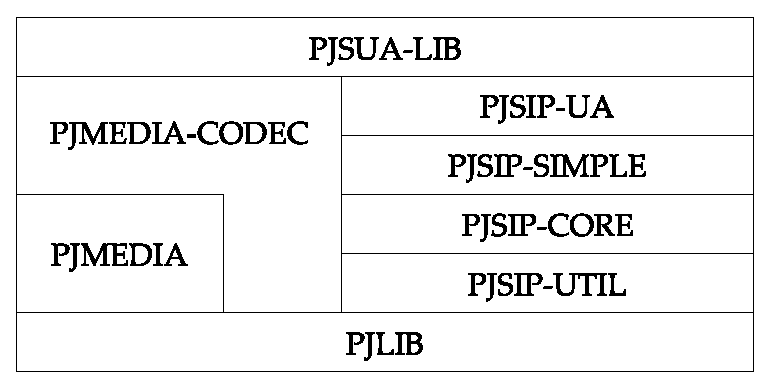
\includegraphics[width=0.70\textwidth]{grafiken/pjsip.eps}
	\caption{�bersicht der Komponenten des PJSIP Protokollstacks}
	\label{fig:pjsip}
\end{figure}

Viele der existierenden SIP Clientanwendungen und Protokollstapel kamen f�r den Prototypen auch deshalb nicht in Frage, weil sie in einer anderen Programiersprache als C oder C++ geschrieben waren und so nicht in das 3D-Framework integriert werden konnten. 

\section{Entwicklungsumgebung}

\subsection{Programmiersprache}
Ich habe mich f�r den Einsatz von C und C++ als Programmiersprache aus mehreren Gr�nden entschieden: Die Darstellung der virtuellen 3D Welt und die die Etablierung, Verarbeitung und Wiedergabe der Audiostr�me bilden zusammen ein Echtzeitsystem. Da in so einem System der gleichzeitige zeitnahe Ablauf mehrerer Prozesse erforderlich ist, wird eine sehr performante Programmiersprache ben�tigt. Es sind vor allem kurze Reaktionszeiten erforderlich, um f�r den Spieler eine glaubw�rdige Illusion zu erzeugen. Beim Audiosignal reichen bereits Verz�gerungen von mehr als 300ms aus, um eine Verst�ndigung unverst�ndlich zu machen. 

Da C und C++ maschinennahe Sprachen sind, und keine Interpretation des Quellcodes w�hrend der Laufzeit ben�tigen, besitzen sie einen Effizienzvorteil gegen�ber Sprachen eine hohe Abstraktionsebene besiezten oder w�hrend der Laufzeit interpretiert werden m�ssen. Gerade deswegen liegen fast alle bisher vorgestellten Protokollstapel und Bibliotheken f�r VoIP oder 3-D Grafik ausschlie�lich in C oder C++ vor. 

\subsection{Testumgebung}
Die wiederkehrenden Tests wurden auf diversen mir zur Verf�gung stehenden Systemen
durchgef�hrt. Als Clients kamen, zwei \textit{AMD Athlon(tm)} X2Dual 4200+, \textit{IBM} \textit{Thinkpad }T42 1,6GHz, \textit{Sony Vaio }CR 1,6GHz und \textit{HP Compaq }6710b 2,1GHz zum Einsatz. Um m�glichst realistische Bedingungen zu schaffen, wurden die Rechner auf verschiedene Art und Weise an das Internet angebunden. Zwei Laptops nutzten ein 54Mbit WLAN mit VPN Anschluss, ein Laptop befand sich hinter einem NAT-Router mit WLAN, die station�ren Rechner verf�gten �ber einen direkten 100Mbit LAN Anschluss. In den Tests nutzten alle Rechner den Breitbandanschluss der Universit�t Mannheim, der �ber 33 MBit Down- und 16 MBit Upload verf�gt. 

Auf den folgenden Seiten soll nun die Umsetzung, der in Kapitel 3 erarbeiteten Konzepte und Verbesserungsvorschl�ge erl�utert werden. Es werden ausgew�hlte Probleme und L�sungswege beschrieben, die in dieser Phase der Arbeit aufgetreten sind. 

\section{3D-Spielewelt mit Irrlicht und Irrklang}

\subsection{Irrlicht}

\subsubsection{Initialisierung}
Zu Beginn des Spieles werden die \textit{Irrlicht} und VoIP Instanzen initialisiert, die sp�ter in zwei verschiedenen Prozessen parallel ablaufen und miteinander zusammenarbeiten. In \textit{Irrlicht} wird die 3D Welt gerendert und die Darstellung und Steuerung des Avatars vorgenommen und in der VoIP Instanz die Audiokommunikation signalisiert und durchgef�hrt.

\subsubsection{Level}
%Todo bild vom Level
\begin{figure}[tbh]
	\centering
		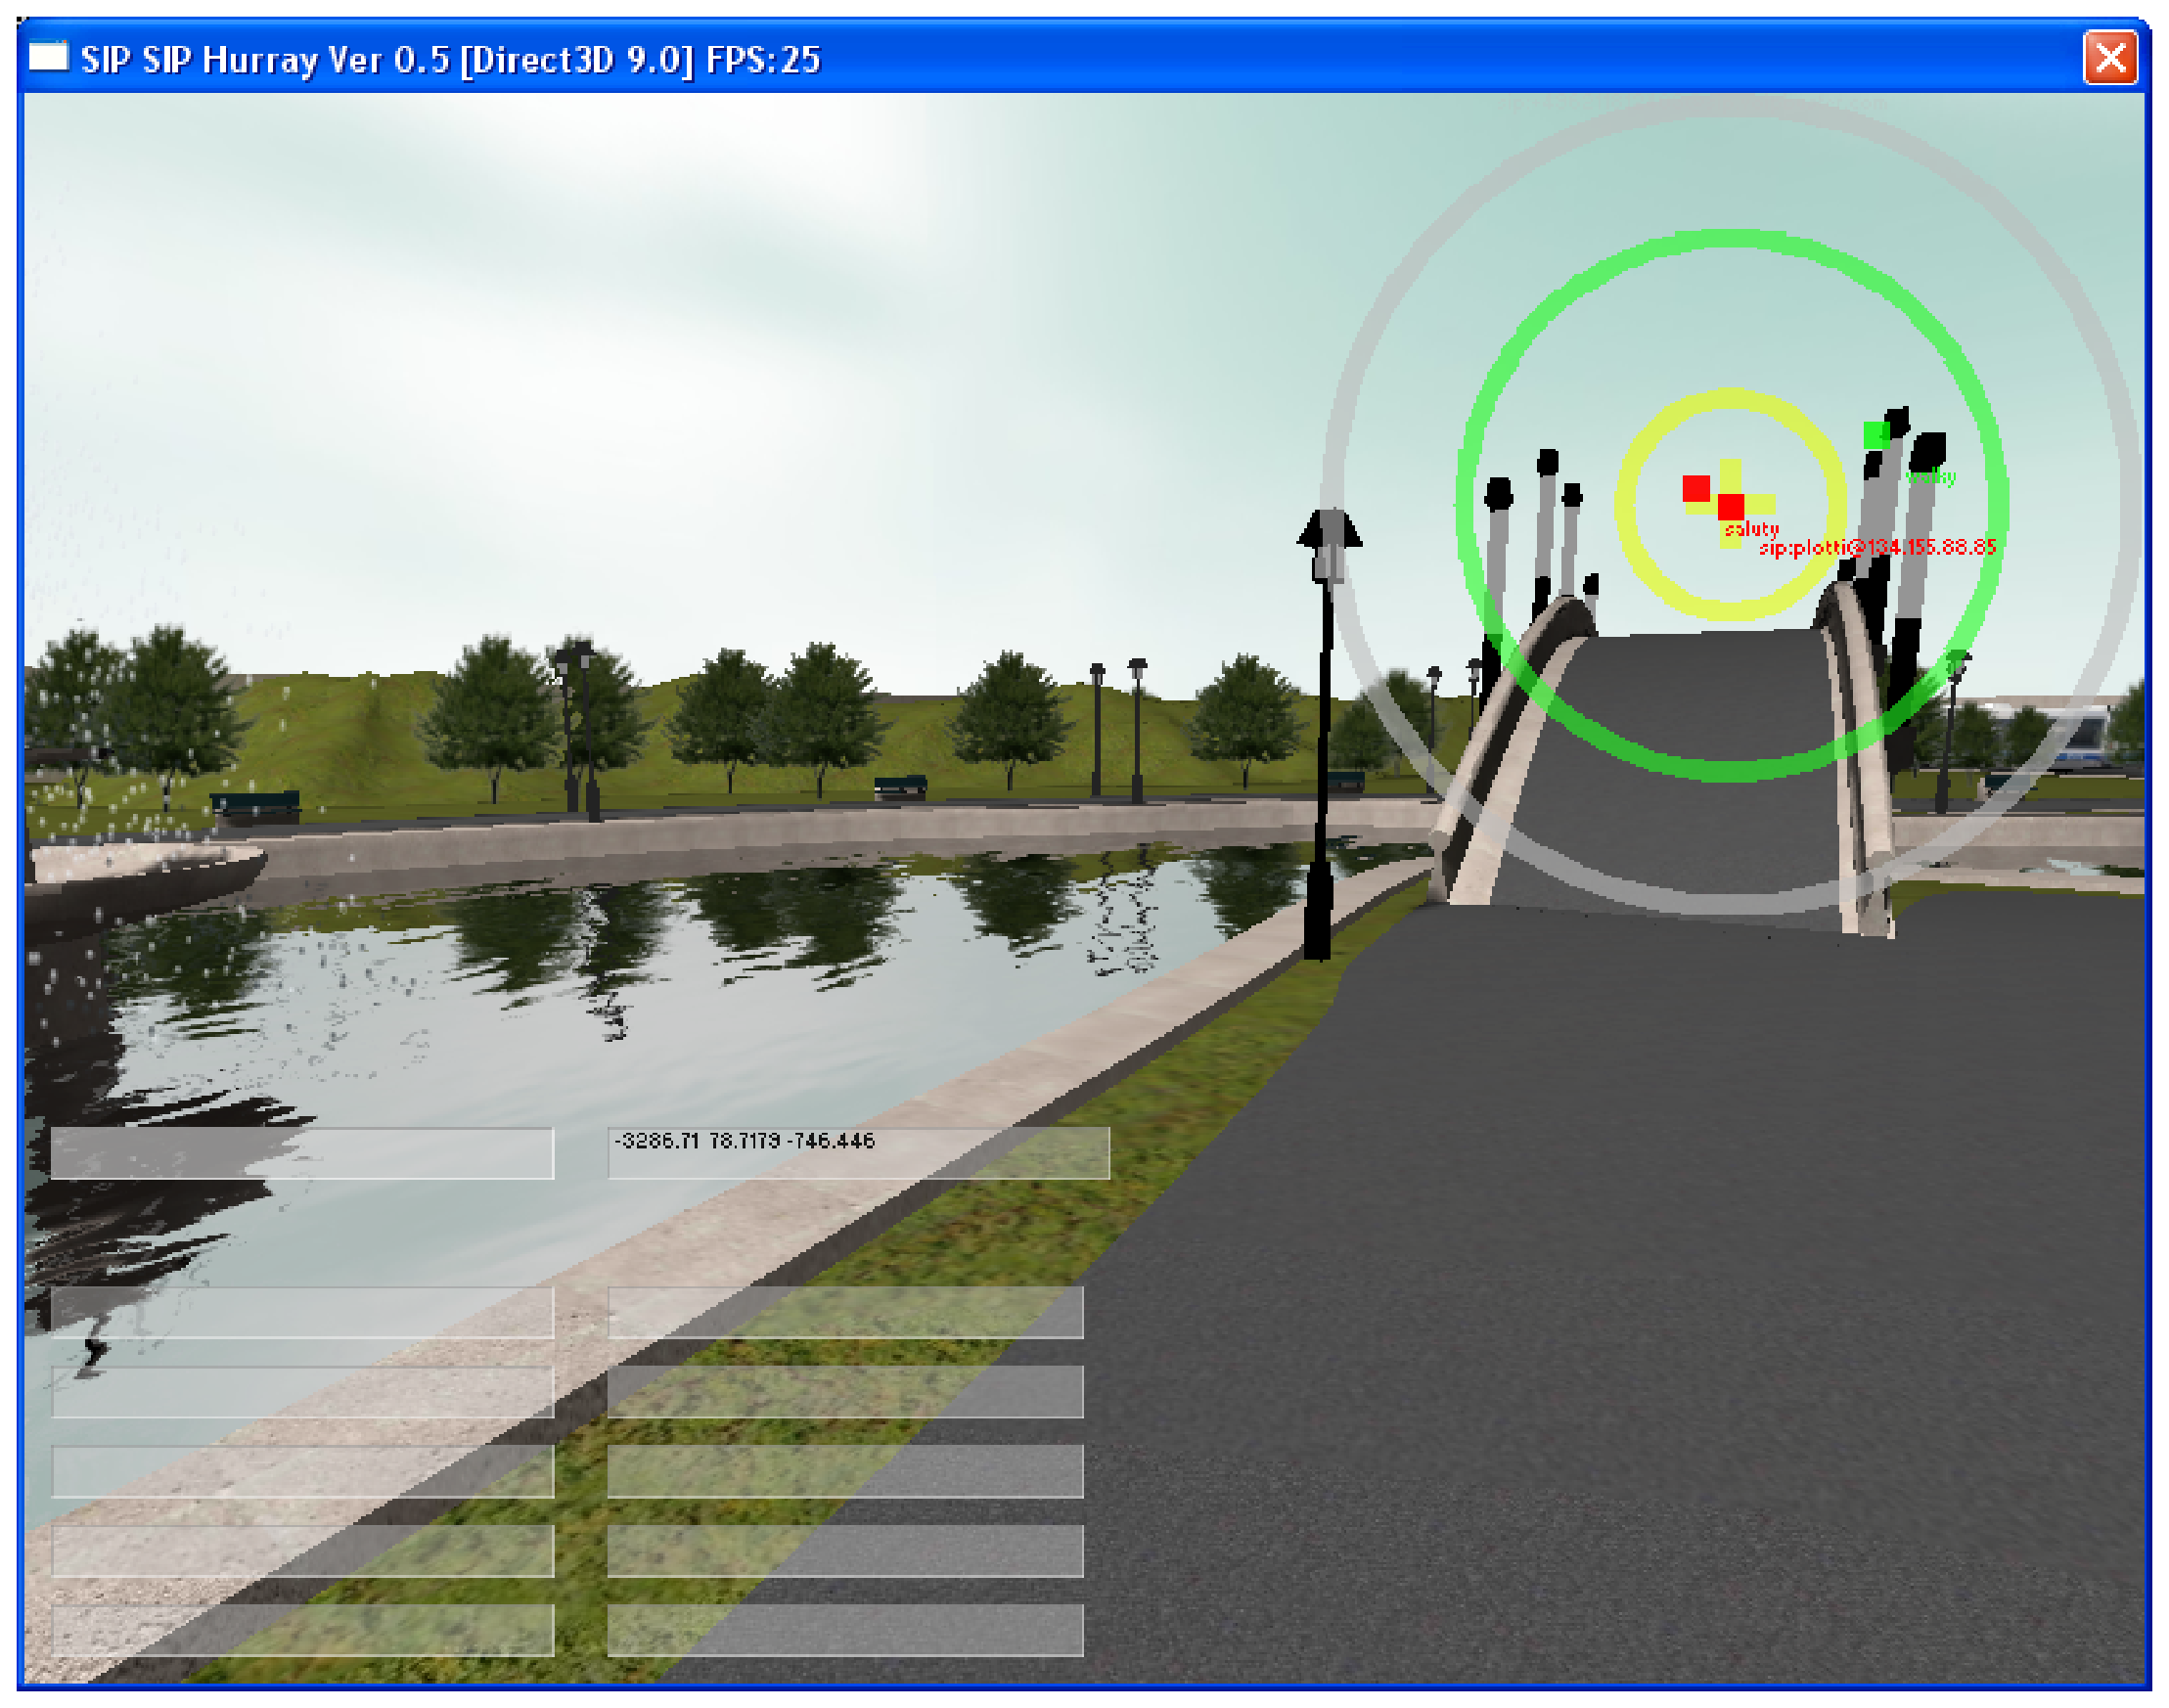
\includegraphics[width=1.00\textwidth]{grafiken/spielewelt-screenshot.eps}
	\caption{Realistische 3D Spielewelt mit Radar}
	\label{fig:spielewelt-screenshot}
\end{figure}

F�r eine m�glichst realistische Umsetzung wurde ein Level benutzt, das einen Park zeigt in dem Spieler die M�glichkeit haben sich frei zu bewegen. Die Vorstellung, dass Menschen in hier spontane Gespr�chen f�hren liegt nahe. Ebenso erscheint in diesem Szenario die �bertragung der Sprache per Luft sehr nat�rlich.

%\subsubsection{\textit{Collision Detection}}
%Der Spieler kann in der Implementierung mit andern Spielern des Levels und dem Level selbst interagieren. Dabei ist es wichtig, dass eine Berechnung der Kollision des Spielers mit dem Level oder anderen Spielern stattfindet, da ohne eine solche der Spieler alle Gegenst�nde durchdringen k�nnte und das Szenario unnat�rlich erscheint. Diese Berechnung wird "`\textit{Collision Detection}"' genannt und wird ebenfalls mit im \textit{Irrlicht} Framework umgesetzt. 

\subsubsection{Steuerung}
Der Spieler ist in der Lage sich in alle Richtungen zu Bewegen und zu springen. Dies erlaubt es ihm sich anderen Spielern zu n�hern, um so die Sprachkommunikation einzuleiten. Bis auf die Steuerung des Avatars sind keine weiteren Tastenkombinationen n�tig, um Sprachkommunikation einzuleiten. Diese findet automatisch statt, wenn der Spieler die entsprechende Distanz zum anderen Spieler unterschritten hat. Dies wird in einem Radar, das die verschiedenen Verbindungsstufen abbildet oben links auf dem Bildschirm angezeigt. Eine Liste unten links zeigt zus�tzlich alle Teilnehmer des Spiels und die Teilnehmer der pers�nlichen Konferenz an. 

\subsubsection{Radar}

In einem Radar am oberen-linken Bildschirmrand werden f�r den Spieler alle Teilnehmer des Spiels angezeigt. Das Radar verf�gt �ber drei Zonen, die die einzelnen Verbindungsstufen repr�sentieren. Spieler werden mit einem Icon und ihrem zugeh�rigen Namen angezeigt. In der �ffentlichen Zone wird das Icon gr�ulich dargestellt, betreten sie die soziale Zone wird dieser gr�n gef�rbt und in der privaten Zone ist ihr Icon gelb. Die Metapher der Luft�bertragung gepaart mit dem Radar als Orientierungshilfe unterst�tzt den Spieler bei der Adressierung von anderen Teilnehmern. Spieler sind direkt in der Lage zu sehen, an wen ihre Sprachnachrichten �bertragen werden und welche Teilnehmer sie gerade h�ren. 

\subsection{\textit{Irrklang}}

\subsubsection{Lokale Audioszene}
Das Level wurde zus�tzlich mit mehreren lokalen Audioquellen ausgestattet, die eine realistische Audioumgebung simulieren. So sind der Wind, der Springbrunnen und die Fahrzeuge des Levels mit entsprechenden Audiodateien unterlegt, die mit Hilfe der Irrklang Engine f�r das Ohr dreidimensional positioniert werden k�nnen. Die Audioszene wird lokal erzeugt und muss im Gegensatz zur Sprachkommunikation nicht �ber das Netzwerk �bertragen werden. Die Sprachkommunikation und die lokale Audioszene existieren simultan und erzeugen so f�r den Spieler ein eine realistische Illusion. 


\section{PjSIP VoIP Instanz}

Die VoIP Instanz unterscheidet zwischen der Signalisierung (PJSIP) und der Kontrolle und Fluss des Audiostroms(PJMEDIA). Es existiert sowohl eine low-level API (PJSIP \& PJMEDIA), als auch eine high-level API(PJSUA). Die gleichzeitige direkte Nutzung der PJMEDIA und PJSIP bildet eine direkte Kontrolle �ber jeden Schritt der Anwendung. DIe PJSUA-API dagegen erlaubt es die Signalisierung, Account-Management, Buddy-Management, Pr�senz, Instant-Messeging, Konferenzen und Medien-Funktionalit�ten zu abstrahieren. 

\subsection{Signalisierung mit PJSUA}
// TODO Vieleicht doch ein bisschen CODE? 

\subsection{Medienfluss}
\begin{figure}
	\centering
		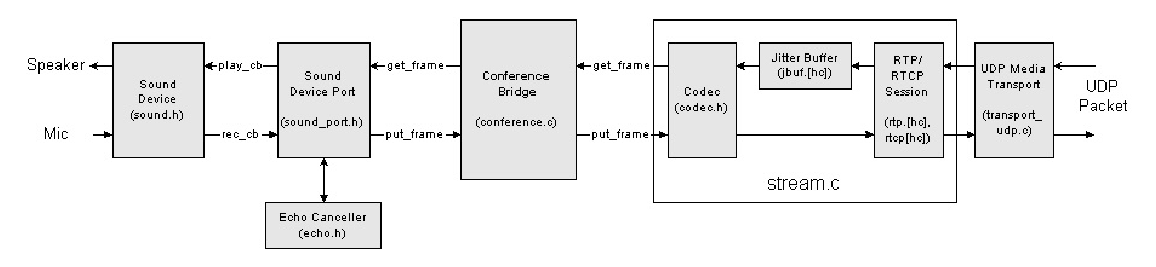
\includegraphics[width=1.00\textwidth]{grafiken/pjsip-mediaflow.eps}
	\caption{Eine �bersicht �ber den Audiofluss in PjSIP}
	\label{fig:pjsip-mediaflow}
\end{figure}

Die Hauptkomponenten der Abbildung \ref{fig:pjsip-mediaflow} bestehen aus:
\begin{itemize}
	\item einem Soundkarten-Port, der eine Abstraktions Ebene darstellt, die die Callbacks der Soundkarte in Audioframes �bersetzt)
	\item einer Conference Bridge, die Operationen auf den Audiosignalen erlaubt
	\item einem Medienstrom, der bei einem Anruf erstellt wird.
	\item einem Medientransport, der f�r die �bertragung des Medienstroms durch RTP/RTCP Pakete zust�ndig ist.
\end{itemize}

W�hrend der Initialisierungsphase, erstellt die Anwendung einen logischen Soundkarten-Port und die Konferenzbr�cke. Diese zwei Objekte bleiben w�hrend der Lebenszeit der Applikation erhalten. Wird ein Anruf get�tigt oder entgegengenommen, erstellt die Anwendung eine Instanz des Media-Transports (normalerweise UDP). Die Adresse(Port) des Media-Transports wird als Parameter der SDP IVITE Nachricht �bergeben (empfangen). Ist die Verbindung etabliert wird eine Medien-Sitzung erstellt. Die Anwendung kann nun den Audiostrom der Medien-Sitzung nutzen und ihn bei der Konferenzbr�cke registrieren. Danach kann dieser Audiostrom-Slot in der Konferenzbr�cke mit anderen Slots anderer Audiostr�me verbunden werden, oder mit dem sog. "`0-slot"', der direkt mit der Soundkarte und dem Mirkofon verbunden ist. 

\section{Zusammenarbeit von \textit{Irrlicht} und VoIP}

\subsection{Aktualisierung der VoIP Instanz}

Im Spiel selbst ist der \textit{Irrlicht Scene Manager} f�r eine Verwaltung aller Objekte der Spielewelt verantwortlich. Er verf�gt sowohl �ber die Koordinaten des Spielers und aller lokalen Objekte, als auch �ber die Koordinaten aller anderen anwesenden Spieler im Spiel. Erh�lt der Spieler neue Positionsinformationen von anderen Teilnehmern, werden diese im \textit{Scene Manager} aktualisiert. Genauso versendet der Spieler selbst seine eigenen Koordinaten an alle teilnehmenden Spieler.

Die Aktualisierung aller Positionsinformationen findet (alle 10 Frames) in der Hauptschleife von \textit{Irrlicht} statt, in der sowohl die 3D Welt als auch die lokale VoIP Instanz aktualisiert wird. Anhand der Koordinaten aller aktiven Spieler des Scene Managers kann die die VoIP Instanz die entsprechenden Distanzvektoren berechnen. Die Anzahl der dargestellten Frames h�ngt dabei stark von der Grafikleistung des Rechners ab und lag bei den Testmaschinen zwischen 5fps und 53fps.
 
Unterschreitet ein Spieler die Entfernung zu einem anderen Spieler, veranlasst die VoIP Instanz einen entsprechenden Anruf zu diesem Teilnehmer. In Abh�ngigkeit der Entfernung voneinander werden die entsprechenden Zonenmechanismen durch die VoIP Instanz im Hintergrund eingeleitet. Hier werden vor allem Callbacks zwischen Irrlicht und der VoIP Instanz genutzt um entsprechende Events auszul�sen. 

\subsection{Buddy Konzept}

Die Spieler im Spiel werden durch Avatare repr�sentiert. Jedem Avatar im Spiel ist ein entsprechender "`Buddy"' in der VoIP Instanz gegen�bergestellt.
Diese h�lt somit eine lokale Liste von eigenen \textit{Buddies} vor. S�mtliche Sprachkommunikation findet durch einen Anruf zum entsprechendem Buddy statt. Falls sich mehrere Personen in der H�rn�he des Spielers befinden, werden auch mehrere Anrufe zu den entsprechenden "`Buddies"' veranlasst. Da f�r jeden Teilnehmer ein eigener Anruf get�tigt und separat verwaltet wird, ist der Spieler in der Lage die Parameter wie Lautst�rke, Bitrate und Codec jedes einzelnen Anrufs zu ver�ndern und neu auszuhandeln. Alle get�tigten anrufe werden in der lokalen \textit{Conference Bridge} abgemischt.

\subsection{Conference Bridge}
Die Aufgabe der \textit{Conference Bridge} besteht die Audiostr�me bestehender SIP Anrufe lokal abzumischen (siehe Abbildung \ref{fig:conference-bridge}. Jeder Teilnehmer der Br�cke verf�gt �ber einen Input und Output Kanal, die beliebig miteinander verschaltet werden k�nnen. Das Mikrofonsignal wird unver�ndert an alle Teilnehmer der \textit{Conference Bridge} �bertragen. Die empfangenen Signale werden jedoch in ihrer Lautst�rke angepasst. Dabei wird die Lautst�rke der jeweiligen Audiostr�me mit dem Parameter $r$ zwischen 0 und 1 gewichtet, bevor sie addiert werden. So kann die Entfernung des Teilnehmers simuliert werden. Die Parameter $r$ wiederum werden anhand der Distanz der Avatare vom Spieler errechnet, die auf einen Bereich zwischen 0 und 1 normiert wird. �berschreiten Spieler im spiel die H�rweite werden die Teilnehmer aus der Konferenzbr�cke entfernt, der logische SIP Anruf jedoch beibehalten. Dieses Verhalten wird sp�ter in Abschnitt \ref{Zonen-Implementierung} beschreiben. Liegen die Audiosignale in verschiedenen Samplingraten vor, �bernimmt die Conference Bridge automatisch ein Resampling des Signals. 

\begin{figure}
	\centering
		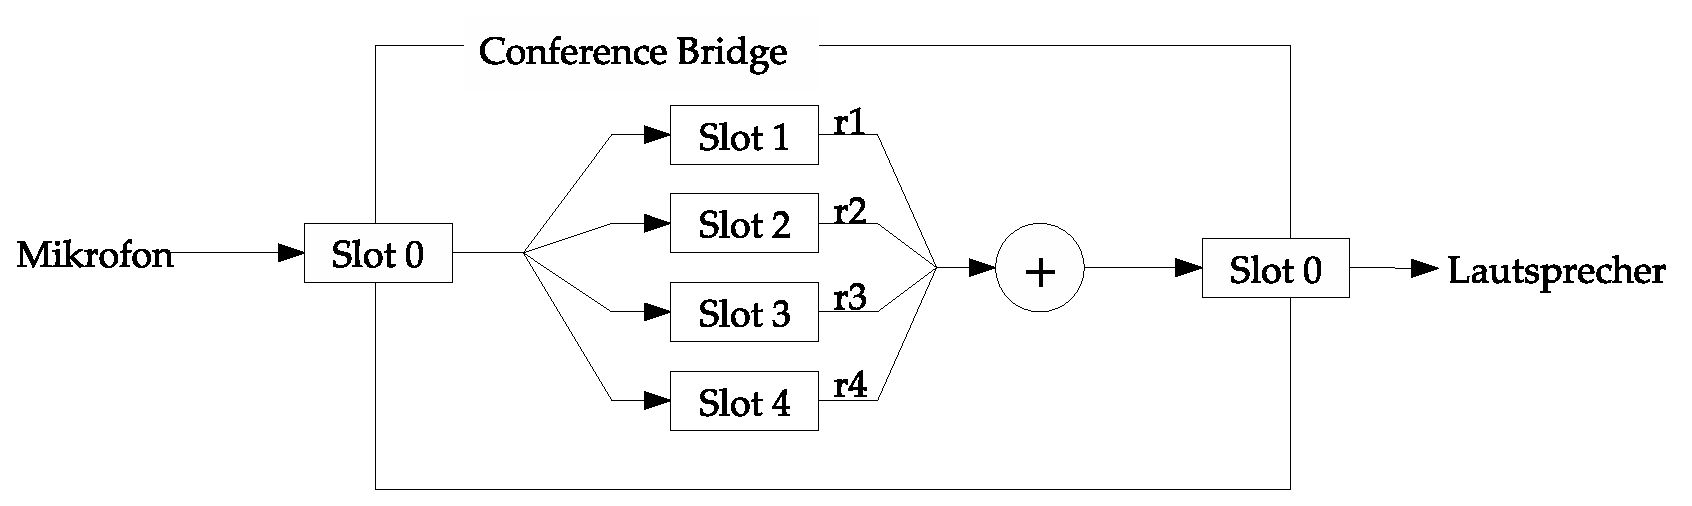
\includegraphics[width=1.00\textwidth]{grafiken/conference-bridge.eps}
	\caption{Funktionsweise der Konferenzbr�cke mit 5 Teilnehmern und Anpassung der einzelnen Audiostr�me}
	\label{fig:conference-bridge}
\end{figure}


\section{Spielablauf}

\subsection{Registrierung}
Bevor das eigentliche Spiel stattfindet, registriert sich der Spieler bei einem voreingestellten Registrar. Dazu sendet er seine Anmeldung gem�� dem im Kapitel 3 vorgestellten Registrierungsprozess. Ist die Registrierung abgeschlossen ist der Registrar in der Lage diesen Spieler erfolgreich zu lokalisieren. W�hrend der Registrierungsphase wird auch ein �ffentlicher STUN-Server kontaktiert, der es dem Spieler erlaubt seine �ffentliche IP Adresse und den Typ des eingesetzten Routers herauszufinden. 

\begin{figure}
	\centering
		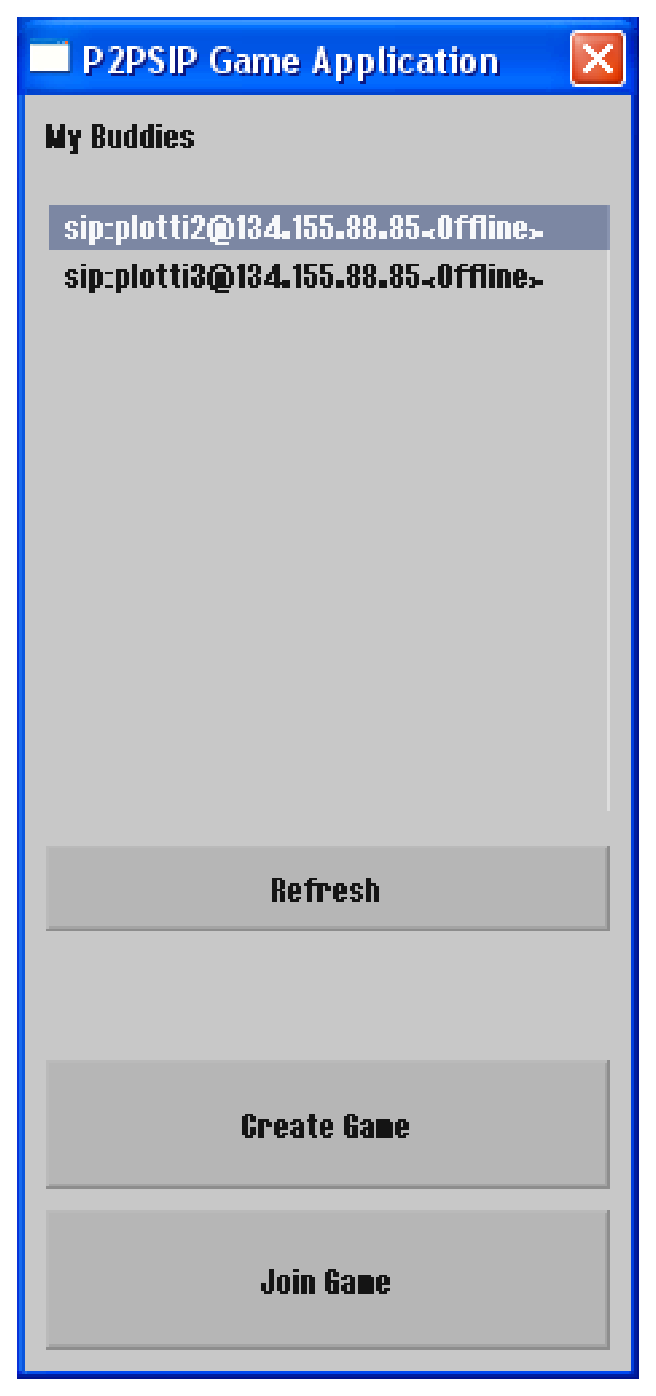
\includegraphics[width=0.3\textwidth]{grafiken/gamestart-screenshot.eps}
		\caption{Startbildschirm des Spiels}
\end{figure}

\subsection{Spieler startet das Spiel}
Auf dem Startbildschirm findet der Spieler seine bisherigen Freunde vor und kann ihren aktuellen Status ablesen: Diese k�nnen entweder offline, online oder gerade im Spiel sein. M�chte der Spieler das Spiel betreten, kann er einen aktiven Spieler anw�hlen und mit dem Dr�cken des \textit{Join}-Knopfs am Spiel teilnehmen. M�chte er ein neues Spiel starten, kann er mit dem Bet�tigen des \textit{Create}-Knopfes ein neues Spiel anlegen. 

\subsection{Neuer Spieler betritt das Spiel}
Betritt ein neuer Spieler das Spiel, so wird er von diesem Zeitpunkt ab vom lokalen \textit{Scene Manager} verwaltet und in der 3D Welt als neuer Avatar dargestellt. Dieser wird f�r jeden neuen Spieler an einer festgelegten Einstiegskoordinate erzeugt. Gleichzeitig wird die SIP Adresse des neuen Teilnehmers in die lokale \textit{Buddyliste} des Spielers aufgenommen. Befindet sich der entsprechende Spieler in H�rn�he, wird ein Anruf zu diesem Teilnehmer in der VoIP Instanz ausgef�hrt.

\subsection{Spieler bewegt sich im Spiel}
Jeder Spieler ist in der Lage sich frei im Level zu bewegen. Jede Bewegung wird allen anderen Teilnehmern mitgeteilt, damit sie in der Lage sind ihre Spielewelt konsistent zu halten. Auf die gleiche Weise erh�lt der Spieler selbst ebenfalls Bewegungsinformationen aller Spieler des aktiven Spiels. Diese Aktualisierung wird alle 10 Frames vorgenommen. Anhand der Positionsinformationen der Spieler wird die Sprachkommunikation entsprechend des Zonenkonzepts eingeleitet.

\subsection{Spieler beendet sein Spiel}
Beendet ein Spieler sein Spiel, so bedeutet es f�r die �brigen Spieler nicht, dass das komplette Spiel f�r sie auch zu Ende ist. Das Verlassen eines Teilnehmers hat zur Folge, dass dieser seine Positionsinformationen nicht mehr versendet und auch keine weiteren mehr empf�ngt. Alle aktiven Gespr�che mit diesem Spieler werden ebenfalls beendet. Eine fr�he Implementierung nutzte spezielle Nachrichtentypen, um dies zu signalisieren. In einer sp�teren Version wurde jedoch der SIP Pr�senzdienst dazu eingesetzt\footnote{Eine genaue Beschreibung dieses Dienstes findet sich in Kapitel 4. Die Implementierung wird in Kapitel 9 erl�utert.}.

\subsection{Verbindungsaufbau}
Befinden sich zwei Teilnehmer in einer entsprechenden H�rn�he, wir diese Bedingung sie dazu veranlassen eine Verbindung untereinander aufzubauen. Dabei findet der Verbindungsaufbau entsprechend des SIP Protokolls statt, besitzt jedoch einen signifikanten Unterschied, der im folgenden erkl�rt werden soll:

M�chte Teilnehmer A zu Teilnehmer B eine Verbindung herstellen, sendet er eine SIP-Nachricht INVITE an Teilnehmer B. Die Nachricht enth�lt die Beschreibung der RTP-Session nach dem SDP Protokoll und alle notwendigen Angaben. Teilnehmer B sendet die gleiche Nachricht da er auch eine Verbindung herstellen m�chte.

Falls ein Teilnehmer die INIVTE Nachricht erh�lt, pr�ft er ob er gerade eine Verbindung zum anderen Teilnehmer aufbaut, oder bereits eine Verbindung aufgebaut hat. Ist das der Fall so antwortet er auf den ankommenden Anruf mit der Response Nachricht 403 Forbidden. Diese Vorgehenswiese weicht vom SIP Standard ab und wird im anschlie�enden Abschnitt behandelt.

Baut Teilnehmer jedoch noch keine Verbindung zum anderen Teilnehmer auf und ist auch nicht mit ihm verbunden, so funktioniert der Rufaufbau wie gewohnt. Hat ein Teilnehmer die Verbindung akzeptiert, sendet er einen SIP-Response 200 OK der vom anderen Teilnehmer mit der Nachricht ACK best�tigt wird. Mit dem Empfang der ACK Nachricht, ist die logische Verbindung abgeschlossen. Nun kann eine Verbindung nach dem Protokoll RTP verlaufen und es besteht eine Sitzung zwischen den Teilnehmern. 

\subsubsection{Das Problem der doppelten Verbindung}
Da Teilnehmer zwar zentral lokalisiert werden jedoch unabh�ngig von einer zentralen Instanz Verbindungen signalisieren k�nnen, kann der Fall auftreten, dass beide Teilnehmer zeitgleich eine Verbindung miteinander aufbauen wollen. Dieser Fall tritt immer dann auf, wenn beide Spieler im Spiel die erforderliche N�he zueinander erreicht haben. Dann versucht sowohl Teilnehmer A eine Verbindung zu Teilnehmer B aufzubauen, als auch Teilnehmer B eine Verbindung zu Teilnehmer A aufzubauen. Dies entspricht dem Problem im Alltag, wenn zwei Personen sich versuchen zur exakt gleichen Zeit anzurufen und jeder nur ein Besetztzeichen h�rt. 

\begin{figure}[tbh]
	\centering
		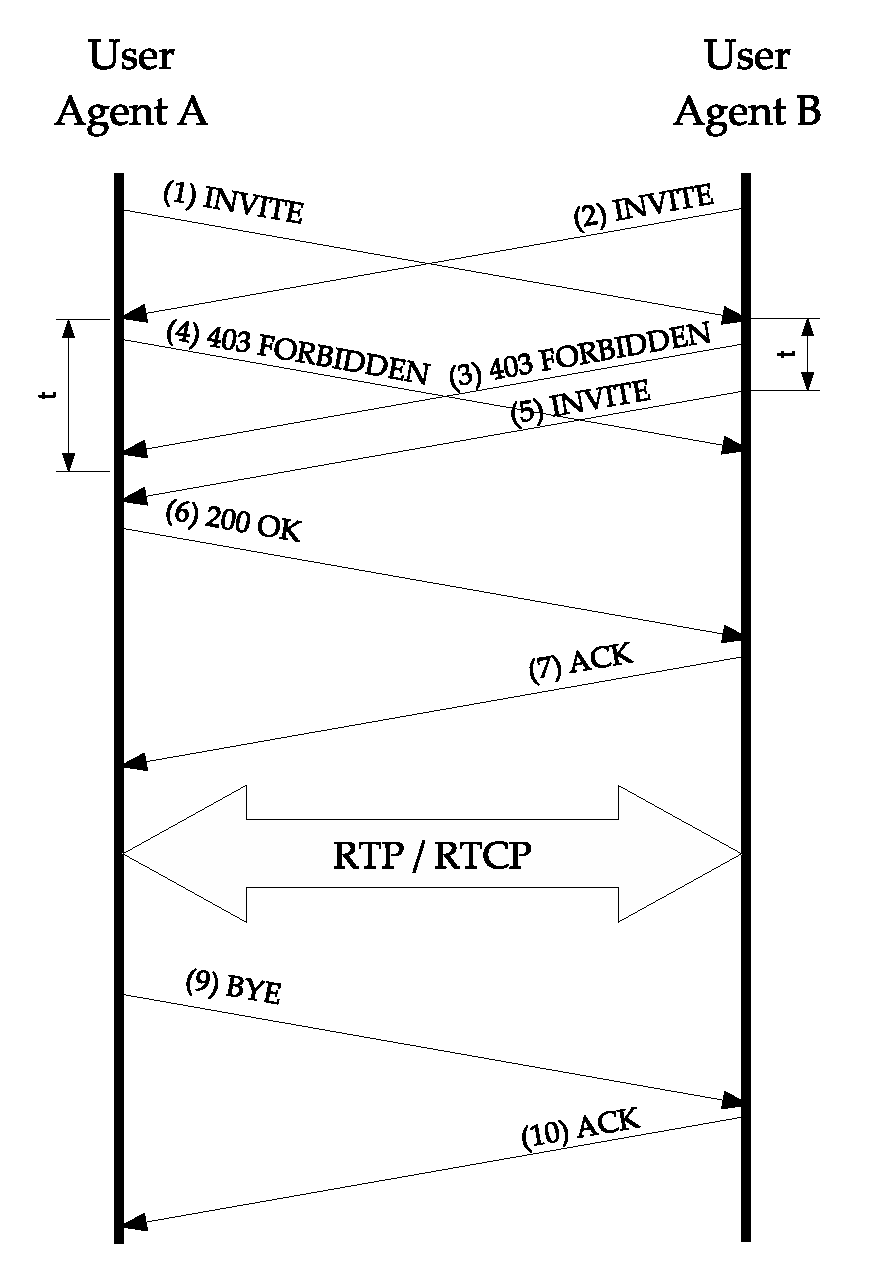
\includegraphics[width=0.60\textwidth]{grafiken/sipanruf_403.eps}
		\caption{Ablauf einer symmetrischen Verbindung}
	\label{fig:sipanruf_403}
\end{figure}

Bei diesem Szenario k�nnen zwei verschiedene F�lle auftreten. Der einfache Fall liegt vor, wenn bei Teilnehmer B eine INVITE Nachricht von A eintrifft und B bereits mit A verbunden ist. Dann kann er den zweiten Dialog einfach verwerfen, da ja bereits eine bestehende Verbindung existiert.

Der kompliziertere Fall ist der symmetrische Fall: Dieser tritt dann ein wenn B, w�hrend er selbst eine Verbindung mit A aufbaut, die INVITE Nachricht erh�lt. Hier hat B hat ebenfalls eine INVITE Nachricht an A geschickt, w�hrend A zur gleichen Zeit auch eine INVITE Nachricht an B geschickt hat. Lehnen nun beide Teilnehmer die Verbindung ab, so f�hrt es dazu dass in diesem Fall �berhaupt keine Verbindung zwischen den Teilnehmern zustande kommt. 

Es ist also wichtig, dass eine gemeinsame Regel f�r alle Teilnehmer existiert nach der beim Dialogaufbau vorgehen. In diesem Fall warten beide Teilnehmer eine zuf�llige Zeit und und versuchen danach eine neue Verbindung zu etablieren bis der unsymmetrische Fall auftritt. Diese Vorgehensweise hat sich in der Praxis bew�hrt. 

\subsection{Verbindungsabbau}
Der Verbindungsabbau findet wie gewohnt statt: Befindet sich Teilnehmer B nicht mehr in Verbindungsreichweite zu Teilnehmer A so beenden beide die Verbindung zueinander. Dazu senden sie eine BYE Nachricht an den anderen Teilnehmer, die mit einer ACK Nachricht best�tigt wird. 

\section{Zonen}
\label{Zonen-Implementierung}
Die Umgebung des Spielers wurde wie gefordert in drei Zonen unterteilt. 

\subsection{�ffentliche Zone}
Die �ffentliche Zone wird genutzt, um SIP Verbindungen des Spielers mit anderen Teilnehmern zu initiieren und so eine Grundkonnektivit�t zwischen diesen herzustellen. Da der Verbindungsaufbau mitunter bis zu 1 oder 2 Sekunden betragen kann, wird diese Zone dazu genutzt um vorab die gesamte Signalisierung vorzunehmen, bevor die Teilnehmer tats�chlich die n�tige H�rn�he eingenommen haben, um miteinander zu sprechen. So soll die entstehende Latenz beim Verbindungsaufbau f�r den Spieler nicht erkennbar sein. 

Durch die Existenz der �ffentlichen Zone findet ein stufenweiser �bergang von nicht verbundenen Teilnehmern, �ber Teilnehmer die bereits auf logischer Ebene verbunden sind, hin zu Teilnehmern, die tats�chlich Audiodaten austauschen statt. 

In dieser Zone werden logische SIP Verbindungen aufgebaut, weil es sehr wahrscheinlich ist, dass die Teilnehmer, die bereits diese Entfernung eingenommen haben auch die soziale Zone betreten werden, in der tats�chlich eine Audioverbindung stattfindet. 

Da Spielergruppen in virtuellen Welten, der Erfahrung nach, w�hrend der Spielesitzung eine geringe Entfernung zu anderen Mitgliedern der gleichen Gruppe beibehalten, soll durch eine �ffentliche Zone sichergestellt werden, dass bereits eine Konnektivit�t zwischen allen Teilnehmern herrscht, damit eine Sprachkommunikation zwischen diesen Spielern verz�gerungsfrei stattfinden kann. Diese Grundkonnektivit�t beansprucht dabei eine minimale Bandbreite, gew�hrleistet aber einen raschen Aufbau der Audiokommunikation. 

\subsubsection{Eingang und Verlassen der �ffentlichen Zone}
Die �ffentliche Zone kann aus zwei Richtungen betreten werden. Wird sie von au�en betreten, wird eine logische SIP Verbindung zwischen den Teilnehmern aufgebaut. Der doppelte Verbindungsaufbau und die entstehenden Probleme wurden oben bereits beschrieben. Findet ein Wechsel von der sozialen Zone zur �ffentlichen Zone statt, muss nur daf�r gesorgt werden dass die Bandbreite reduziert wird, w�hrend der logische SIP Anruf erhalten bleibt.

In der Implementierung wurden zwei Mechanismen ausprobiert, um einen geringen Bandbreitenverbrauch in dieser Zone zu gew�hrleisten ohne jedoch die logische SIP Verbindung zu beenden. Dabei wurden die speziellen Eigenschaften der verwendeten Protokolle SIP und RTP ausgenutzt.

\subsubsection{RTP - Silence Supression}
W�hrend der logische SIP Anruf weiterhin erhalten bleibt, wird auf auf RTP Ebene kein weiteres Audiosignal mehr �bertragen. Dies geschieht, in dem die Teilnehmer aus den jeweils lokalen lokalen Konferenz genommen werden und so das Mikrofonsignal nicht mehr �bermittelt wird. 

Da kein Audiosignal mehr an die gegenseitigen Spieler �bertragen wird, wird von nun an eine \textit{Silence Suppression} vorgenommen. Dieses Verhalten entspricht der im Kapitel 3 geschilderten Eigenschaften der \textit{Silence Supression} des RTP Protokolls. Das geschilderte Verhalten hat aber den Unterschied, dass die \textit{Silence Supression} nicht von der tats�chlichen Stille im Mikrofon abh�ngt, sondern von der Entfernung der Teilnehmer untereinander. 

Diese Methode bietet die M�glichkeit, den Bandbreitenverbrauch in dieser Zone auf unter 1kB/s \footnote{Messungen zum Bandbreitenverbrauchs in dieser Zone finden sich in Kapitel 10.} zu reduzieren. Der gro�e Vorteil dieses Verfahrens besteht darin, dass der Wechsel zwischen der �ffentlichen und sozialen Zone verz�gerungsfrei stattfinden kann, da kein neues Aushandeln der Parameter ben�tigt wird.

\subsubsection{SIP - HOLD}
Eine Reduzierung des Bandbreitenverbrauch wurde auch mit der SIP HOLD Funktionalit�t ausprobiert. Hierbei signalisiert das SIP Protokoll, dass der Anruf geparkt werden soll und die RTP Verbindung w�hrend des Hold Vorgangs beendet wird. Wird der Hold aufgehoben, wird die RTP Verbindung wieder neu etabliert. Die Messergebnisse\footnote{Siehe Kapitel 9} und eigene Erfahrungen haben gezeigt, dass zwar eine noch gr��ere Einsparung der Bandbreite als bei der RTP Silence Supression stattfindet da praktisch keine Daten mehr �bertragen werden. Der Nachteil jedoch besteht darin, dass beim Wiederaufnehmen des Anrufs eine sp�rbare Verz�gerung auftritt, da die Verbindungsparameter des Gespr�chs wieder neu verhandelt werden m�ssen.

\begin{figure}[tbh]
	\centering
		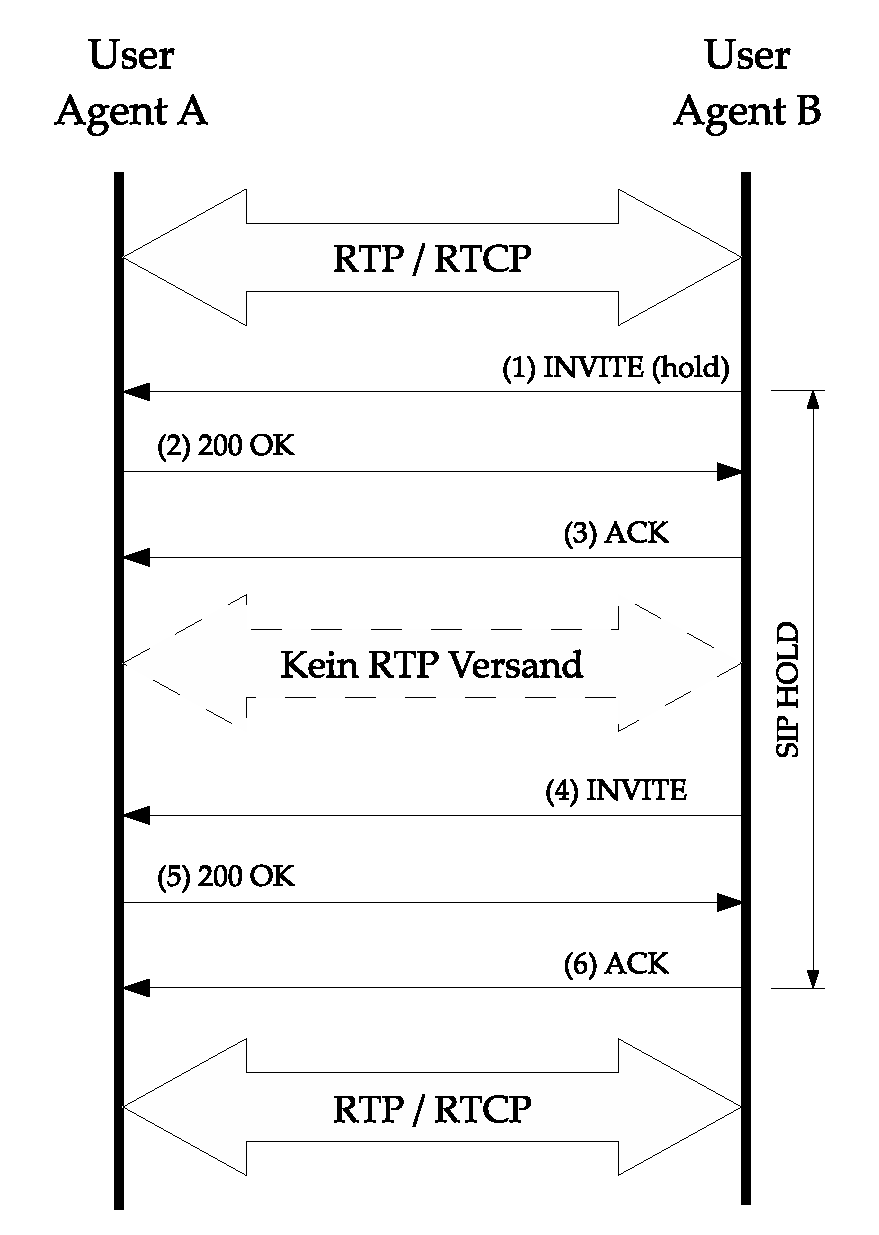
\includegraphics[width=0.60\textwidth]{grafiken/siphold.eps}
	\caption{Schematischer Ablauf des SIP-HOLD Nachrichtenverlaufs}
	\label{fig:siphold}
\end{figure}

\subsection{Soziale Zone}
In der Sozialen Zone werden die Teilnehmer, der bereits aufgebauten Verbindungen der  eigenen lokalen Konferenz hinzugef�gt. Innerhalb dieser Konferenz wird die Lautst�rke der Teilnehmer gem�� ihrer Entfernung angepasst. Audiosignale von Teilnehmern, die sich am inneren Rand der sozialen Zone des Spielers befinden werden unged�mpft mit einer Lautst�rke von 100\% abgemischt. Diese nimmt linear in Abh�ngigkeit der Entfernung zu den Spielern ab, bis sie am �u�ersten Rand der Zone 0\% betr�gt. 

\subsubsection{Lautst�rkenanpassung}
Da die Lautst�rke der �bertragenen Stimme bei einer �bertragung durch Luft mit zunehmender Entfernung abnimmt wurde ein einfaches physikalisches Modell der Schall�bertragung benutzt: Generell gilt, dass Schalldruck bei zunehmender Entfernung $r$  mit $1/r$ abnimmt. Da sich die Schallintensit�t auf eine immer gr��er werdende gedachte Kugeloberfl�che (proportional zur Entfernung $r$) verteilt, nimmt sie mit der Entfernung quadratisch ab. 

Zu Testzwecken wurden sowohl die lineare als auch die quadratische Abnahme der Schallintensit�t modelliert, um festzustellen welche Ver�nderung nat�rlicher erscheint. Die lineare Abnahme erwies sich sich als transparenter f�r den Benutzer, da eine einfachere Relation zwischen Lautst�rke und Entfernung hergestellt werden konnte. 

Als ein Problem bei der Lautst�rkenanpassung erwies sich die unterschiedliche Aufnahmelautst�rke der Mikrofone. Da verschiedene Mikrofone eine unterschiedliche Sensibilit�t haben, senden Spieler unter Umst�nden bei gleicher Entfernung verschieden laute Signale. In einem fertigen Produkt, sollte das Mikrofon dynamisch auf einen bestimmten Pegel normiert werden, bevor das Spiel beginnt. Solche Verfahren sind Standard bei VoIP Telefonen und k�nnten sp�ter leicht nachger�stet werden. %http://www.sengpielaudio.com/Rechner-entfernung.htm

\subsubsection{Audiocodec}
In der sozialen Zone wird ein Audiocodec mit einer niedrigen Bitrate eingesetzt, um eine gr��ere Anzahl an m�glichen Mitspielern zu erm�glichen. In den Testszenarios habe ich mich f�r den Speex Codec mit einer Abtastrate von 16kHz und einer Bitrate von 11 Kb/s entschieden, der einen MOS Wert von �ber 4 liefert. Es ist nat�rlich vorstellbar auch qualitativ schlechtere Codecs mit einer noch geringeren Bitrate einzusetzen, um dem Spieler noch mehr Verbindungen zu erm�glichen. Diese Entscheidung kann in einem fertigen Produkt entweder dem Spieler selbst - bei einer manuellen Konfiguration - �berlassen werden oder automatisch anhand der verf�gbaren Bandbreite bestimmt werden. So k�nnten Spieler mit einer h�heren Bandbreite auch ein besseres Audiosignal verbreiten, w�hrend Spieler mit einer schwachen Anbindung nur Codecs mit einer niedrigen Bitrate einsetzen k�nnten.

\subsection{Private Zone}

\subsubsection{Lautst�rke}
In der privaten Zone A bleibt die Laut\-st�rke der Teilnehmer konstant bei 100\%. Dies erm�glicht den Teilnehmern sich in einem kleinen Radius umeinander zu bewegen, unt trotzdem immer noch mit einer optimalen Lautst�rke zu kommunizieren. 

\subsubsection{Audiocodec}
Zus�tzlich dazu ist in einem Testszenario eine weitere Unterscheidung zur sozialen Zone getroffen worden, indem in der privaten Zone ein qualitativ h�herwertiger Codec mit einem gr��eren MOS Wert verwendet wird. Diese Vorgehensweise soll daf�r sorgen, das Mitspieler in unmittelbarer N�he besonders gut verst�ndlich sind. Im Gegensatz zur Sozialen Zone wird erwartet, dass nur wenige Spieler diese Zone betreten, da angelehnt an die Erkentnisse aus Kapitel 2 Menschen in virtuellen Welten �hnliche Distanzzonen einnehmen wie im realen Leben. In der Implementierung wurde in einem Testszenario f�r die private Zone der Speex Codec mit einer Abtastrate von 32 kHz verwendet, w�hrend in der Sozialen Zone der Speex Codec mit einer geringen Abtastrate von 8kHz eingesetzt wurde. 

\section{PTSN Netzwerke}
Durch die M�glichkeit SIP Server mit externen Gateways zu verbinden, wurde auch die Metapher des Festnetz-Telefons umgesetzt, dass dem Spieler tats�chlich erlaubt aus der virtuellen Welt in die reale Welt zu telefonieren. Dazu wurde das Modell einer Telefonzelle auf dem Spielfeld platziert. Befindet sich der Spieler in unmittelbarer N�he zu dieser Telefonzelle, findet ein Anruf an eine beliebige Telefonnummer statt. Dieses \textit{Proof of Concept} zeigt, dass mit Hilfe eines standardisierten Protokolls solche M�glichkeiten sehr einfach realisiert werden k�nnen. 
\newpage~
\chapter{SIP als Netzwerkschicht f�r Spiele}

Wie schon in Kapitel 7 beobachtet, sind die Herausforderungen an die Verwaltung einer Sprachkommunikation mit der darunter liegenden Netzwerkarchitektur verbunden. Vor allem in Kapitel 6 wurde deutlich, dass die Signalisierung und Lokation der Teilnehmer einer Konferenz, genauso wichtig ist wie der Austausch der Audiodaten selbst. Es liegt daher nahe, die bereits eingesetzten Komponenten nicht nur dazu zu Nutzen, um Teilnehmer zu Lokalisieren und Konferenzen zu steuern, sondern auch um Spieleinformationen zu �bertragen. 

\section{SIP als Netzwerkschicht}

Da es sich bei SIP um generisches Protokoll handelt, ist es prinzipiell nicht nur f�r die Sprachkommunikation einsetzbar sondern auch, um beliebige Sitzungen zwischen Clients zu etablieren und Daten in Echtzeit auszutauschen. Dieses Kapitel soll zeigen, welche der bestehenden Client-Server und Peer-to-Peer Architekturen sich mit SIP umsetzen lassen. Es ist keineswegs das Ziel bestehende Probleme der einzelnen Architekturen l�sen, indem das SIP-Protokoll verwendet wird, sondern vielmehr eine standardisierte Adressierung,  Signalisierung und hohe Abstraktionsebene zu erreichen.

In diesem Kapitel werden zun�chst Client-Server Konzepte und dann eine die Implementierung einer Client-Server Architektur auf Basis des SIP Protokolls vorgestellt. Diese soll zeigen, dass es sehr einfach ist einen Spielprototyp zu bauen,  bei dem SIP f�r die Sprachkommunikation und als Netzwerkschnittstelle eingesetzt wird. 

Im zweiten Teil werden bisherige Konzepte f�r Peer-to-Peer Spiele dargestellt und abschlie�end die Funktionsweise von P2PSIP n�her erl�utert, um zu zeigen wie ein P2PSIP Overlay gestaltet werden kann. 

\section{Anforderungen an die Netzwerkschicht}

Mehrspieler-Spiele besitzen vielf�ltige Anforderungen an eine Netzwerkarchitektur. Abh�ngig von der gew�hlten Architektur lassen sich einige der Anforderungen leichter umsetzen als andere.

\textbf{Sicherheit:} Da Spieler gegeneinander antreten, sollte Manipulation ausgeschlossen werden. Dazu ben�tigt man eine sichere Kommunikation zwischen den Spielern. 

\textbf{Persistenz:} Das Spiel kann z.B. Objekte enthalten die nur genau einmal existieren. Deswegen muss zwischen den einzelnen Sitzungen daf�r gesorgt werden, dass diese dauerhaft gespeichert werden auch wenn der Benutzer sich unerwartet vom System abmeldet.

\textbf{Zuverl�ssigkeit:} Durch einen zu h�ufigen Ausfall des gesamten Systems wird die Spielerfahrung negativ beeinflusst. 

\textbf{Konsistenz:} Um eine sinnvolle Interaktion zwischen Spielern zu erm�glichen, muss die Erfahrung dieser Welt f�r jeden Mitspieler konsistent sein. Dies beinhaltet das Aufrechterhalten von Spielezust�nden und die Synchronisation von Ereignissen. Um eine Konsistenz der Spielewelt zu erreichen, m�ssen Ereignisse der Spieler mittels Nachrichten im System ausgetauscht werden. 

\textbf{Reaktionsfreudigkeit:} Da Spiele oft die echte Welt simulieren, hat die Reaktionsfreudigkeit des Systems gro�en Einfluss darauf, f�r wie realistisch diese Welt gehalten wird. Werden durch zu gro�e Verz�gerungen Ereignisse zu sp�t dargestellt, so wird die Spielmechanik gest�rt. 

\textbf{Skalierbarkeit:} Eine skalierbare Architektur sollte eine gro�e Anzahl und  Anstieg an gleichzeitigen Benutzern unterst�tzen, ohne dass die Last des Systems dramatisch ansteigt. 

W�hrend Client-Server basierte Systeme eine hohe Sicherheit, Persistenz und Konsistenz bieten, ist ihre Zuverl�ssigkeit und Skalierbarkeit durch den Einsatz einzelner zentralen Komponenten limitiert. Peer-to-Peer-basierte Systeme dagegen bieten eine hohe Skalierbarkeit und Zuverl�ssigkeit, sind aber anf�llig in ihrer Sicherheit, Persistenz und Leistung. 

In der Forschung werden beide Architekturen bez�glich der oben genannten Aspekte untersucht. So existieren viele Studien \cite{lau06} zur Skalierbarkeit von Client-Server- und Peer-to-Peer-Architekturen, die bez�glich ihrer Bandbreite, Last und des Delay verglichen werden. Auch Inhalte des Netzwerkverkehrs in Spielen \cite{lau05b}, oder die Auswirkungen der geografischen Verteilung von Spieleservern und Spielern wurden untersucht \cite{feng03}. 


\section{Client - Server in Netzwerkspielen}
Die Client-Server-Architektur f�r Netzwerk-Spiele war �ber Jahrzehnte die dominierende Architektur, die in der Lage war, zwischen 2 und 64 Spielern gleichzeitig zu unterst�tzen \cite{singhal99}. 

In einem Client-Server Modell ist der Server f�r die Verwaltung des Spielstandes verantwortlich. Die Clients auf Spielerseite werden genutzt, um den Spielstand anzuzeigen und mit dem Server zu kommunizieren. Jedes Ereignis auf dem Client wird an den Spieleserver �bertragen, der entsprechende Spieler �ber dieses benachrichtigt. Der Spieleserver verwaltet auch den Beitritt und das Verlassen von Spielern. 

Die Mehrheit kommerzieller Mehrspieler-Spiele benutzt heutzutage eine zentralisierte Architektur, da sie viele Vorteile gegen�ber anderen Architekturen bietet. Diese wird auch in Zukunft die �blichste Architektur f�r Spiele mit einer kleinen Spieleranzahl bleiben, ist aber nicht in der Lage mehrere tausend gleichzeitige Spieler zu unterst�tzen. Obwohl einzelne Server dem System hinzugef�gt werden k�nnen, steigt die Netzwerklast des Systems polynomiell mit der Zunahme von Spielern auf dem System \cite{lau06} an.  

Da die Tendenz zum Spiel als Kommunikationsplattform geht, bei der mehrere Millionen Spieler gegeneinander antreten, aber zentralisierte Systeme nicht �ber mehrere zehntausend Spieler skalierbar sind, verfehlen sie laut Marktanalysten ihr eigentliches Marktpotenzial \cite{thor03}. 

\subsection{Techniken zur Skalierung}

\subsubsection{Sharding}
Um das Problem der unzureichenden Skalierbarkeit zu umgehen, wird von vielen Entwicklern das so genannte "`Sharding"' eingesetzt \cite{brandt05}. Ein "`Shard"' ist eine komplette und unabh�ngige Instanz der Spielewelt. Die maximale Anzahl an Spielern einer solchen Welt ist limitiert.  Durch das Hinzuf�gen von Shards k�nnen Entwickler zwar mehr Spieler aufnehmen, die aber in verschiedenen Spielewelten existieren und nicht miteinander interagieren k�nnen. Das derzeit weltweit gr��te MMOG\textit{World of Warcraft (WoW)} \footnote{Blizzard Entertainment, Version 22.03.2008, http://blizzard.co.uk/} setzt erfolgreich Sharding ein, um Spieler in mehreren gleichzeitig existierenden Spielewelten zu verwalten.

\subsubsection{Clustering}
Eine zus�tzliche M�glichkeit besteht darin, Cluster von Computern einzusetzen, die als gemeinsame Server-Plattform nach au�en auftreten. Solche Systeme werden als \textit{Federated-Client-Server}-Systeme bezeichnet. Diese Methode wird erfolgreich von Spielen wie EVE Online\footnote{CCP hf., Version 04.05.2008, http://www.eve-online.com} eingesetzt, die den Rekord f�r die gr��te Anzahl an gleichzeitigen Spielern auf einem Cluster mit 23000 Spielern h�lt \cite{brandt05}. Dabei ist jeder Server in diesem Cluster f�r eine andere Portion der virtuellen Welt verantwortlich. Durch \textit{Load Balancing} werden Spieler zwischen Servern im Cluster transferiert, um die maximale Bandbreite und Last einer Maschine nicht zu �berschreiten. Studien von Lau \cite{lau06}, in denen das \textit{Client-Server-Federating} simuliert wurde, zeigten jedoch, dass diese Technologie ihre Grenzen hat.

\subsubsection{Interest-Management}
Um eine konsistente Spielewelt zu erzeugen, die performant und skalierbar ist, wird  das \textit{Interest-Management} eingesetzt \cite{morse96}. Unter \textit{Interest Management} versteht man, dass Individuen nur einen begrenzten Wahrnehmungsradius besitzen und nur an Dingen interessiert sind, die in einer limitierten lokalen Umgebung geschehen, welche auch als \textit{Area of Interest} bezeichnet wird. 

Eine �bliche Technik im \textit{Interest-Management }besteht darin, die Spielewelt in Regionen aufzuteilen, wobei der Spieler immer nur Mitglied einer Region ist und auch nur Nachrichten dieser Region erh�lt. \textit{Interest Management} ist in einer Client-Server-Architektur sehr einfach umsetzbar, da der Server alle eingehenden Nachrichten vor dem weiterleiten filtern kann, was jedoch in einem P2P System nicht ohne weiteres m�glich ist, da keine solche zentrale Komponente existiert \cite{yu05}.

\section{Implementierung einer Client-Server Architektur mit SIP}
Der Spieleprototyp verf�gt �ber keinen ausgefeilten Spielemechanismus, da die Entwicklung eines solchen �ber den Rahmen der Arbeit hinausgeht. Dazu m�ssten die oben angesprochenen Punkte der Persistenz, Sicherheit, Konsitenz und Fairness detailliert behandelt werden. 

Stattdessen werden im Prototyp nur �nderungen der Positionen der Spieler periodisch (alle 100ms) �bertragen und die Spielewelt lokal aktualisiert. Das einzige "`Ziel"' des Spiels besteht darin, sich mit anderen Spielern zu unterhalten. Jeder Teilnehmer ist in der Lage sich in einer 3D Umgebung zu bewegen, und mit den Gegenst�nden und Spielern eines Spieles zu kollidieren. Mit Hilfe der SIP Netzwerkschicht sollen alle Spieler �ber Ereignisse anderer Spieler informiert werden. 

Bei der Implementierung einer SIP Netzwerkschicht wurde versucht bereits bestehende Komponenten einzusetzen. Proxy und Registrar wurden als eine zentrale Einheit eingesetzt, die als Serverinstanz fungiert. Die Registrierung der Benutzer wird vom Registrar vorgenommen und der Proxy wird genutzt, um alle Nachrichten zu empfangen und an die entsprechenden Teilnehmer weiterzuleiten. 

Hat sich ein Spieler erfolgreich auf dem Registrar angemeldet, so wird bei eingehenden Nachrichten die Zieladdresse dieses Benutzer auf dem Proxy aufgel�st und an den entsprechenden Client weitergeleitet. Um Nachrichten zwischen Teilnehmern zu verschicken wird das wird SIP SIMPLE-Protokoll eingesetzt. Der Datenaustausch zwischen den Teilnehmern findet mit Hilfe des SIP \textit{MESSAGE}-Nachrichtentyps statt. Der SIMPLE-Pr�senzdienst wird genutzt, um festzustellen welche Spieler aktiv am Spiel Teilnehmen und Nachrichten empfangen sollen. 

%Abbildung die den Nachrichtenfluss zeigt. 
%Registrierung am Registrar
%Nachrichtenfluss mittels MESSAGE so eine Art Knotennetz oder sowas.
 
\subsection{SIP SIMPLE Protokoll}

% A Framework for Conferencing with the
% Session Initiation Protocol (SIP)
% http://www.ietf.org/rfc/rfc4353.txt

\subsubsection{Nachrichtendienst}
Beim SIP SIMPLE-Protokoll handelt sich um ein offenes, weit verbreitetes Protokoll der SIP-Protokollfamilie, f�r das viele Open-Source Implementierungen existieren und das auch in kommerziellen L�sungen, wie dem \textit{MSN-Messenger}\footnote{Microsoft, Version 20.03.2008, http://messenger.live.com}, eingesetzt wird. 

Der Einsatz von SIP-SIMPLE als Netzwerkschicht, um Spieledaten auszutauschen, ist deshalb m�glich, weil es sich dabei um ein generisches Protokoll handelt, das f�r verschiedene Zwecke genutzt werden kann. Obwohl es urspr�nglich vorgesehen wurde, um Instant Messenging im SIP Standard zu erm�glichen, kann es genauso genutzt werden um Spieledaten auszutauschen. Die \textit{MESSAGE}-Nachrichtentypen enthalten im Body-Teil statt Textnachrichten die Koordinaten der Spieler oder deren Status. 

Exemplarisch wurden mehrere Nachrichtentypen implementiert:
\begin{itemize}
	\item \textbf{Position}: Die \textit{Positionsnachricht} enth�lt die aktuelle Position des Spielers im Spiel. Ihr Aufbau besteht aus der X, Y und Z Koordinate, denen die Buchstabenfolge COORD vorausgeht.
	\item \textbf{Rotation}: Die \textit{Rotationsnachricht} enth�lt die aktuelle Rotation des Spielers im Spiel. Ihr Aufbau besteht aus der X,Y und Z Drehrichtung, denen die Buchstabenfolge ROTATION vorausgeht.
	\item \textbf{Animation}: Die \textit{Animationsnachricht} enth�lt die aktuelle Animation des Spielers im Spiel. Diese wird anhand verschiedener Statuscodes in der Nachricht mitgeteilt. Ihr Aufbau besteht einem Statuscode, dem die Buchstabenfolge ANIMATION vorausgeht. 
\end{itemize}

Der Proxy dient nur als Nachrichtenverteiler, dh. er selbst enth�lt keinerlei Spielelogik. Stattdessen sind alle Spieler selbst daf�r verantwortlich, anwesende Mitspieler mit allen relevanten Informationen �ber sich zu versorgen. Dies geschieht, indem sie in periodischen Zeitabst�nden (alle 100ms) ihre Positions- und Rotationsdaten\footnote{In Abh�ngigkeit davon, in wie gro�en Zeitabst�nden die Informationsupdates versendet werden, braucht die Kommunikation weniger oder mehr Bandbreite. Eine Auswertung der verbrauchten Bandbreite findet sich in Kapitel 10}. an alle Teilnehmer verschicken und bei einer �nderung ihrer Animation auch eine Animationsnachricht versenden. 

Entsprechend dieses Prinzips erwarten Teilnehmer, dass alle anderen Spieler sich gleich verhalten und sie mit ihren Informationen versorgen. Durch dieses Vorgehen existiert kein spezieller Spieler, der das Spiel veranstaltet und steuert. So ist es m�glich, dass jederzeit Spieler das Spiel verlassen und betreten k�nnen, ohne dass das aktuelle Spiel unterbrochen wird.

\subsubsection{Buddy Konzept}
Der vom Spieler gew�hlte Benutzername, entspricht auch seiner SIP Adresse, �ber die er erreicht werden kann. W�hlt beispielsweise der Spieler mit der IP:192.168.0.50 den Benutzernamen "`bob"', so werden Anfragen an seine SIP Adresse sip:bob@ip-registrar beim Proxy auch an diese IP weitergeleitet. Mit Hilfe des Lokationsdienstes kann jeder Teilnehmer diesen Spieler unter seinem Alias erreichen. 

In einer lokalen \textit{Buddy Liste} werden die SIP Adressen aller bekannten Teilnehmer gespeichert. Betreten neue Teilnehmer das Spiel, so wird ihre Adresse zu dieser Liste hinzugef�gt. Mit Hilfe dieser Liste und des Pr�senzdienstes sind Spieler in der Lage festzustellen, welche Personen am Spiel teilnehmen und welche nicht. 

Damit die Kommunikation erfolgreich funktionieren kann, muss jeder Teilnehmer �ber eine vollst�ndige \textit{Buddy Liste} verf�gen. In der Implementierung wird diese Tatsache vorausgesetzt. Diese Aufgabe muss in einem tats�chlichen Spiel die Spielemechanik �bernehmen, die daf�r sorgen muss, dass jeder Teilnehmer �ber eine aktuelle Liste aller Teilnehmer verf�gt.

Eine einfache M�glichkeit k�nnte darin bestehen, dass der Registrar beim Anmeldevorgang eines neuen Teilnehmers alle bisherigen Spieler dar�ber informiert, dass ein neuer Spieler das Spiel betreten hat. Der neue Spieler w�rde ebenfalls eine Liste aller bisherigen Teilnehmer erhalten, damit er diese �ber seine Ereignisse informieren kann. 

Hier zeigt sich auch der Vorteil einer zentralen Instanz, bei der der Lokationsdienst  eine aktuelle Liste aller Spieler besitzt und der Pr�senzdienst auch deren Status kennt. Zus�tzlich k�nnen an dieser zentralen Stelle die Konsistenz, Persistenz,Rechtemanagement und andere f�r ein tats�chliches Spiel essentiellen Aufgaben durchgef�hrt werden. Diese w�ren in einem Peer-to-Peer System nicht so einfach zu realisieren.

\subsubsection {Pr�senzdienst}
Pr�senz ist ein Begriff, der im Instant Messaging verwendet wird. Er bezieht sich darauf, dass Benutzer feststellen k�nnen, ob andere Benutzer mit dem Dienst verbunden sind. Falls dies der Fall ist, kann eine Benachrichtigung erfolgen, die anzeigt, ob diese Benutzer \textit{online} oder \textit{offline} sind. 

Der Pr�senzdienst wird im Prototypen deshalb eingesetzt, damit Spieler feststellen k�nnen welche andere Teilnehmer sich im aktuellen Spiel befinden und mit Informationsupdates versorgt werden m�ssen. 

Publish- und Subscribe-Mechanismen sind in Mehrspieler-Computerspielen ein beliebtes Schema, bei bei dem Clients bei einem Spieleserver oder auch einzelnen Clients Ereignisse abonnieren \cite{mercury02}. Die Notify Nachrichten werden bentutzt, um den Spielestatus zu �bertragen, der bei den Clients sp�ter angezeigt wird.

Zu diesem Zweck wird die \textit{SUBSCRIBE/NOTIFY} Funktion von SIP benutzt, die bereits in Kapitel 4 beschrieben wurde. Der SIMPLE-Pr�senzdienst nutzt genau diese Nachrichtentypen und erlaubt es so Teilnehmern, ihre eigene Pr�senz zu signalisieren (\textit{NOTIFY}) und Pr�senzen anderer Teilnehmer zu abonnieren (\textit{SUBSCRIBE}). Anhand dieser Pr�senzinformation werden nur Nachrichten nur an Spieler versandt, die eine Teilnahme am Spiel signalisiert haben. 

Dazu wurden in der Implementierung drei einfache Pr�senzstati definiert:
\begin{itemize}
	\item \textbf{Offline} - Der Spieler ist nicht an einem Registrar angemeldet und kann auch nicht kontaktiert werden. 
	\item \textbf{Online} - Der Spieler hat sich an einem Registrar angemeldet, nimmt aber momentan nicht am Spiel teil.
	\item \textbf{Im Spiel} - Der Spieler hat sich am Registrar angemeldet und nimmt gerade am Spiel teil.
\end{itemize}

Startet der Spieler das Spiel, so teilt er als erstes dem Pr�senzserver seinen \textit{Online-Status} mit. Wenn sich der Spieler dann im Startbildschirm befindet, abonniert er zun�chst die Pr�senz aller seiner Eintr�ge in der Buddy-Liste. Somit ist er in der Lage zu sehen, welche Teilnehmer f�r ein Spiel in Frage kommen. Betritt der Spieler ein Spiel, so signalisiert er dem Pr�senzserver die �nderung seines Status zu \textit{"`Im Spiel"'}. Der Pr�senzdienst teilt diese �nderung allen Spielern mit, was dazu f�hrt, dass diese ab jetzt ihre Informationsupdates an diesen Spieler senden. Der Spieler selbst f�ngt auch an seine Informationsupdates an alle Spieler zu verschicken, die sich \textit{Im Spiel} befinden.

Hierbei ist zu erw�hnen, dass Teilnehmer nur die Pr�senz von Teilnehmern abonnieren k�nnen, die sie auch kennen. Wie oben bereits angesprochen, muss der Spielemechanismus sp�ter diese Aufgabe �bernehmen. Bisherige Spieler m�ssen �ber neue Spieler benachrichtigt werden, damit sie deren Pr�senzstatus abonnieren k�nnen und so Informationsupdates an diese versenden k�nnen.

\subsection{Skalierbarkeit}
Die oben vorgestellten Client-Server-Skalierungskonzepte sind unter SIP in einer einfachen Form auch vorstellbar: Um das Konzept des Sharding umzusetzen, kann bei einem solchen Aufbau f�r jede Spielewelt ein zentraler SIP-Server eingesetzt werden, der eine maximale Anzahl an Spielern erh�lt. F�r ein Clustering-Konzept k�nnen mehrere Registrare beim Anmelden eingesetzt werden, was bereits in Absatz \ref{mehrereregistrare} diskutiert wurde. Da Registrare und Proxys untereinander routen k�nnen ist es m�glich Nachrichten von Benutzern zu empfangen, die sich bei anderen Servern angemeldet haben. Um Interestmanagement umzusetzen, k�nnen beim Proxy Nachrichten gefiltert werden.

\subsection{Tauglichkeit als Peer-to-Peer Ansatz}
Der implementierte Ansatz braucht einzig die zentrale Komponente des Registrars, der f�r die Lokation der Teilnehmer verantwortlich ist. Diese SIP-Komponente l�sst sich theoretisch auch verteilt realisieren, was den Einsatz von SIP als Netzwerkgrundlage f�r Peer-to-Peer-Spiele oder auch einen komplett dezentralen Sprachkommunikationsdienst erm�glicht (siehe Kapitel \ref{peer-to-peer-unicast}). Bevor der theoretische Einsatz von P2P SIP beschrieben wird, sollen zun�chst bestehende Ans�tze f�r P2P Spiele vorgestellt werden.

\section{Peer-to-Peer}
In den letzten Jahren sind Peer-to-Peer Netzwerke ein wichtiger Gegenstand der Forschung geworden \cite{lau05}. Ihr gr��ter Vorteil gegen�ber zentralisierten Architekturen ist ihre Skalierbarkeit. Jeder Knoten, der dem System betritt und Anfragen stellt, muss dem System gegen�ber auch Ressourcen freigeben und Anfragen anderer Knoten bearbeiten. Knoten, die mehr Dienste zur Verf�gung stellen werden als \textit{SuperPeers} oder \textit{Koordinatoren} bezeichnet. Dabei wird eine Gruppe von Knoten als \textit{Overlay} bezeichnet und die konstante Ver�nderung der Teilnehmer als \textit{Churn}. %Es existieren P2P Systeme die bis zu mehreren Millionen an gleichzeitigen Benutzern skalieren \cite{stutzbach05b}. 

\subsection{Distributed Hash Tables}
Als verteilte \textit{Hash-Tabelle}(\textit{Distributed hash table (DHT)}) versteht man eine Datenstruktur, die versucht das allgemeine Problem in P2P-Systemen � den Speicherort einer gesuchten Datei zu finden � mit m�glichst geringem Aufwand effizient zu l�sen. Datenobjekte werden m�glichst gleichm��ig �ber die Knotenmenge verteilt und ein von jedem beliebigen Einstiegsort ortsunabh�ngiges Routing zum verantwortlichen Knoten erm�glicht. Jeder Knoten ist dabei analog zu einem Beh�lter einer Hash-Tabelle. Die Datenstruktur muss st�ndige Anpassungen durch Ausfall, Beitritt und Austritt von Knoten �berstehen, sich selbst organisieren und skalierbar sein. Die Grundlage f�r verteilte Hashtabellen bilden konsistente Hash-Funktionen.

Dazu werden einheitliche zuf�llige Hash-IDs in einem Set von Knoten in einem gro�en Bezeichnungsraum vergeben. Objekten werden eindeutige einheitliche Schl�ssel aus dem gleichen Namensraum zugeteilt. Es existieren folgende Umsetzungen verteilter Hashtabellen: CAN \cite{Ratnasamy01}, Chord \cite{Stoica01}, Pastry \cite{Rowstron01} und Tapestry \cite{zaho01} die sich durch spezielle Eigenschaften voneinander unterscheiden, deren Erl�uterung jedoch nicht Thema der Arbeit ist. 

\subsection{Peer-to-Peer in Netzwerkspielen}
Im Kontext von Netzwerkspielen, kann jeder Spieler als ein P2P-Knoten angesehen werden, der Ressourcen im System freigibt. In der Forschung finden sich erste Anf�nge im P2P-Spiel MiMaze, in dem durch Spieler �ber Ereignisse mittels IP-Multicasting benachrichtigt wird \cite{diot99}. 

Grunds�tzlich lassen sich Peer-to-Peer-Systeme in unstrukturierte Systeme und strukturierte Systeme unterscheiden\cite{lau05}. Unter unstrukturierten Systemen wird ein P2P Overlay verstanden, in dem die Topologie einer zuf�lligen Organisation entspricht und der Inhalt mittels verschiedener Suchverfahren, die das Overlay durchqueren, lokalisiert wird. Dazu analysiert jeder Knoten die Suchanfrage und leitet sie weiter falls er den gew�nschten Inhalt nicht finden kann, was zu einer ineffizienten Lokalisierung f�hren kann (\textit{Flooding}).

Unter einem strukturiertem System versteht man ein P2P-Overlay, in dem die Topologie fest kontrolliert wird und der Inhalt nicht bei zuf�lligen Knoten platziert wird, sondern an speziellen ausgew�hlten Knoten existiert, um seine Lokalisierung mittels DHT effizienter zu erm�glichen. 

Douglas schl�gt in \cite{douglas05} vor P2P-Netzwerk-Architekturen in nachbarbasierte oder regionsbasierte Systeme zu unterscheiden, wobei nachbarbasierte Systeme in die Kategorie der unstrukturierten Systeme fallen und regionsbasierte Systeme zu den strukturierten Systemen geh�ren.

\subsection{Nachbarbasierte P2P-Systeme}
Nachbarbasierte Systeme bestehen aus Knoten mit gleicher Verantwortung, bei der jeder Knoten seine Nachbarn �ber Ereignisse informiert. Einige bekannte Vertreter sind Kawaharas' "`Peer-to-Peer Message Exchange Scheme"' \cite{kawahara02} oder das Keller's Solipsis-System\cite{Keller03}. Die ben�tigte Bandbreite ist eine Funktion der Dichte der Avatare. Solche Systeme besitzen gute Skalierungseigenschaften, k�nnen jedoch durch eine Partitionierung des Netzwerks leiden \cite{Keller03}. Ein Beispiel f�r Partitionierung ist, wenn sich ein Knoten in die N�he eines anderen Knoten begibt, aber keiner der Knoten �ber diese �nderung informiert wird, was letztendlich zu einer fehlerhaften Spielmechanik f�hrt.  Ein weiteres Problem ist die ineffiziente Nutzung der vorhandenen Ressourcen.

%In Kawaharas' "`Peer-to-Peer Message Exchange Scheme"'-Ansatz werden zwischen unmittelbar benachbarten Knoten Nachbarschaftslisten ausgetauscht. Dabei steigt die Gr��e der ausgetauschten Nachrichten mit $O(N^{2})$, wobei $N$ die Anzahl der Nachbarn darstellt \cite{kawahara02}. Dadurch, dass nur unmittelbare Nachbarn Nachrichten austauschen, kann f�r isolierte Gruppen, die sich weit von anderen Gruppen befinden, eine Partitionierung auftreten. 

%In Kellers' Solipsis Ansatz agiert jeder Knoten als Beobachter der benachbarten Knoten \cite{Keller03}.Jeder Teilnehmer beobachtet jede Bewegung seiner Nachbarn und benachrichtigt andere Teilnehmer, wenn neue Nachbarn f�r ihn entdeckt wurden. Im Gegensatz zu Kahawaras Ansatz verbindet sich hier der Teilnehmer nicht unbedingt mit seinen n�chsten Nachbarn.

\subsubsection{Voronoi-basierte P2P-Systeme}
In voronoibasierten Systemen ermittelt jeder Knoten anhand eines Voronoi-Diagramms  seine direkten Nachbarn. Mit allen Nachbarn h�lt der Knoten Verbindungen aufrecht. 
Nachbarn, die sich an der Grenze der \textit{Area of Interest} befinden �berpr�fen wiederum, ob der Knoten sich in den Bereich ihrer Nachbarn bewegt und versorgen diese mit neuen Topologieinformationen \cite{hu04}. 

%Im Voronoi-Schema von Hu \cite{hu04} aktualisiert jeder Teilnehmer bei jeder seiner Bewegungen seine Nachbarn. 

\subsection{Regionsbasierte Peer-to-Peer Systeme}
Regionsbasierte Systeme unterteilen die Welt in geometrische Formen wie Quadrate oder Sechsecke. Regionen k�nnen dabei dynamisch oder statisch sein, der Einfachheit halber werden oft statische Regionen eingesetzt. F�r jede Region wird ein Koordinator oder \textit{Superpeer} bestimmt. Dieser Knoten verwaltet Spieler, die diese Region betreten und verlassen. Dazu werden verteilte Hash-Tabellen genutzt, um weitere Knoten zu finden. Solche Regionen sind daf�r verantwortlich, wor�ber der Spieler informiert wird - alle Ereignisse, die in einer Region generiert werden, werden auch nur an Knoten der gleichen Region propagiert. Eine Ausnahme bildet der Fall, wenn sich ein Knoten von einer Region in die n�chste bewegt und so Ereignisse des Knotens an zwei Regionen propagiert werden. 

Ein Koordinator einer solchen Region, muss dazu nicht unbedingt Teilnehmer des aktiven Spiels sein. Das erm�glicht den Einsatz von dedizierten Rechnern mit gro�en Kapazit�ten, die speziell nur diesen Zweck erf�llen.

Einige Ans�tze f�r regionsbasierte P2P-Systeme sind das \textit{SimMud}-System von Knutnsson et Al. \cite{knutsson04}, der \textit{Zoned-Federation-of-Game-Servers}-Ansatz von Limura at Al. \cite{Iimura04} oder auch ein Skype-basierter Ansatz von Triebel et Al. \cite{triebel07g}.

%Die Regionsgr��e ist ein wichtiger Faktor, beim Entwurf von regionsbasierten Architekturen. Einerseits f�hrt eine Verkleinerung der Region dazu, dass weniger Ereignisse verwaltet und gesendet werden m�ssen. Andererseits f�hren zu kleine Regionen dazu, dass Avatare schnell zwischen Regionen wechseln und so zus�tzliche Nachrichten an benachbarte Regionen gesendet werden m�ssen. 

%Studien von Knutsson, Lu, Xu und Hoptkins \cite{knutsson04} in denen die DHT Architektur auf ihren Einsatz in Mehrspieler Spielen untersucht zeigten, dass die Erzeugung einer �bergangslosen Welt problematisch sein kann. Gerade bei �berg�ngen von einem Koordinator zum N�chsten, kann das Problem auftreten, dass Avatare kurzzeitig nicht mit den n�tigen Informationen �ber die neue Region versorgt werden. Indem Spieler auch die Informationen von benachbarten Regionen abonnieren, k�nnen nahtlose �berg�nge zwischen den einzelnen Regionen erm�glicht werden, wie sie auch im Prototyp \textit{SimMud} demonstrieren. 

%Limura, Hazeyama und Kadobayashi \cite{Iimura04} unterteilen die Spielewelt in Spiele- Zonen, die von \textit{Koordinatoren} verwaltet werden. Diese sind Teil einer "`F�deration"' von \textit{Koordinatoren}, die alle untereinander Spielezust�nde mit Hilfe von DHT austauschen. DHT hilft auch Spielern, die neu hinzukommen oder sich bewegen, ihren zust�ndigen Koordinator zu finden. Die Kommunikation zwischen Spielern findet immer ausschlie�lich mittels eines \textit{Koordinators} statt. 

%Triebel, Guthier und Effelsberg schlagen in \cite{triebel07g} den Einsatz von \textit{Skype} vor, um Spieledaten auszutauschen. Dazu unterteilen sie die Spielewelt in Regionen, denen Spieler angeh�ren k�nnen. Aktionen der Spieler in der gleichen Region, werden ebenfalls nur Spieler der gleichen Region weitergeleitet.F�r jede Region wird mit Hilfe der Skype Chatraum Funktion festgehalten, welche Spieler dieser Region angeh�ren. Die Evaluation des Verfahrens zeigt, dass der Einsatz von Skype f�r Mehrspieler Spiele m�glich ist. 

\subsection{Unstrukturierte und strukturierte Peer-to-Peer-Systeme}
In einigen P2P-Systemen werden sowohl unstrukturierte als auch strukturierte Methoden gleichzeitig eingesetzt. So k�nnen Vorteile von strukturieren Overlays wie DHT werden mit denen von unstrukturierten P2P Architekturen verbunden werden. Ein Knoten kann seine Nachbarn mit Hilfe des Koordinators bestimmen, die zu denen er sich ab dann direkt verbindet. Ein Beispiel stellt der Ansatz von Yu \cite{yu05} dar. 

%Ein Beispiel eines hybriden Systems stellt der Ansatz von Yu \cite{yu05} dar, in dem Knoten in \textit{Master-, Slave-} und \textit{Home-} Knoten unterteilt werden. Master-Knoten sind f�r die Verwaltung der Spielregionen verantwortlich. Home-Knoten helfen Master-Knoten mit Hilfe von DHT sich miteinander zu verbinden und Slave-Knoten werden von den Master-Knoten verwaltet. Im Unstrukturieren Teil tauschen die Master-Knoten zus�tzlich Informationen �ber ihre Nachbarn untereinander aus. Durch diesen Ansatz soll eine Partitionierung des Netzwerks verhindert werden, w�hrend der zus�tzliche Netzwerkverkehr durch die Verwendung von DHT minimiert werden soll.
%TODO TABLE

\section{Hybride Systeme}
Hybride Systeme benutzen einen zentralen Server, um Knoten zu lokalisieren. Der Service selbst wiederum, findet direkt zwischen den Knoten statt. Das beste Beispiel eines hybriden P2P Systems sind Dateiaustauschdienste wie \textit{BitTorrent}\footnote{BitTorrent, Inc, Version 22.05.2008, http://www.bittorrent.com}. Jeder Knoten ver�ffentlicht eine Liste seiner Dateien an einen zentralen �ffentlichen Server. Ein Benutzer, der nach einer speziellen Datei sucht, kontaktiert zun�chst den �ffentlichen Server, um den entsprechenden Knoten zu bestimmen. Der Dateiaustausch hingegen findet zwischen den einzelnen Knoten statt. Ein anderes Beispiel ist der Einsatz von �ffentlichen Registraren beim SIP Protokoll, die f�r die Lokalisierung und Verwaltung der Benutzer verantwortlich sind. Das Telefongespr�ch selbst findet aber zwischen den einzelnen Knoten direkt statt. 

Beide Systeme sind sehr gute Beispiele daf�r, dass der hybride Ansatz funktioniert und sehr gut skaliert \cite{torrent06}. Sie haben jedoch den Nachteil, dass sie im Gegensatz zu komplett dezentralisierten Systemen einen \textit{Single Point of Failure} besitzen.  Um einen \textit{Single Point of Failure} zu vermeiden, werden seit einiger Zeit im Bittorrent Protokoll sog. \textit{trackerlose Torrents}\footnote{BitTorrent Draft, Version 22.03.2008, http://www.bittorrent.com/trackerless.html} auf der Basis von Kademila \cite{kademilla02} einsetzt. Einen �hnlichen Ansatz, bietet der Peer-to-Peer SIP Ansatz, der die Abstraktion von zentralisierten Lokationsdiensten beibeh�lt, aber diese Instanz verteilt realisiert. Dieser Ansatz soll nun im folgenden Abschnitt vorgestellt werden, da er aufgrund seiner generischen Eigenschaften auch f�r P2P-Spiele Einsetzbar ist. 

\section{Peer-to-Peer-SIP}
Peer-to-Peer-SIP ist ein gutes Beispiel f�r einen strukturierten Overlay, der auch die M�glichkeit bietet unstrukturierte Anfragen zu realisieren. Er bietet nicht nur eine hohe Abstraktionsstufe, sondern kann auf bestehenden Standards aufbauen. Somit bietet er eine gute Grundlage um als Netzwerkschicht f�r P2P Spiele zu fungieren. 

\subsection{Motivation f�r Peer-to-Peer-SIP}
Da sich SIP bereits als Standard etabliert hat und viele Eigenschaften besitzt, die es f�r einen reinen Peer-to-Peer-Betrieb attraktiv machen, bestehen seit dem Jahr 2005 Bem�hungen das Hybride SIP Protokoll komplett zu einem reinen Peer-to-Peer Protokoll zu erweitern. Das Interesse an einem solchen Ansatz ist sehr hoch, wie bereits dutzende Entw�rfe\cite{bryan07}, die bei der IETF eingegangen sind, zeigen. 

Der gro�e Vorteil gegen�ber anderen Systemen liegt in der Kombination von bereits etablierten Standards, wie dem SIP und SIMPLE Protokoll, mit Eigenschaften von Distributed Hash Tables. Da bisher in P2P-Systemen noch keine Standards existieren bietet sich die Verwendung von SIP f�r diesen Zweck an, da es als ausgereift und etabliert gilt. Zus�tzlich werden zunehmend Endger�te wie Firewalls oder NAT-Router mit Application Layer Gateways (ALG) ausgestattet. Dies sind zwischengeschaltete SIP-Proxys, die f�r reibungslosen Transfer der SIP-Signalisierung und -Medienstr�me sorgen.

SIP wurde konventionell so gestaltet, dass so viel Funktionalit�t wie m�glich in den Endpunkten enthalten ist. Alle Nachrichten, die f�r den Aufbau eines Telefongespr�chs notwendig sind, werden bereits nur zwischen den Clients ausgetauscht. Das Aushandeln der Audiocodecs, der F�higkeiten der einzelnen User Agents findet ebenfalls direkt zwischen den Endpunkten statt. Ist ein Telefongespr�ch etabliert, so flie�en die Daten direkt zwischen den Teilnehmern. 

Der einzige zentralisierte Baustein in SIP besteht aus der Lokation der Teilnehmer, die vom Registrar vorgenommen wird. In einer gew�hnlichen SIP Konfiguration meldet sich jeder Endpunkt bei einem Registrar an, der eine Zuordnung zwischen dem Namen des Teilnehmers und seiner IP Adresse herstellt. M�chte ein Benutzer einen anderen anrufen, so kontaktiert er zun�chst den Registrar, um die Zieladresse herauszufinden.

\subsection{Funktionsweise}
Es existieren bisher 2 Varianten um ein P2P SIP Umzusetzen. Die vorgestellte Variante nutzt einen Chord-DHT Ring um Knoten anzuordnen. Alternativ zum vorgestellten Verfahren bestehen auch Bem�hungen beim Peer-to-Peer-SIP das CAN-DHT-Verfahren \cite{pundkar07} einzusetzen. Hier wird die Verteilung der Knoten auf in einem zweidimensionalen-Raum abgebildet, was auch der Verteilung der Spieler in einer virtuellen Welt entsprechen w�rde.

Alle Varianten haben gemeinsam, dass die einzige zentrale Komponente des Systems entfernt wird und dezentral zwischen den einzelnen Teilnehmern verteilt mit \textit{DHT} realisiert wird und jeder Knoten einen Teil der Funktionalit�t �bernimmt. 

Dazu werden zwei 2 Arten von IDs verwendet: Eine \textit{Peer-ID}, die den Rechner identifiziert und eine \textit{Ressource-ID}, die den Benutzer identifiziert. Die Information dar�ber, wo eine Person gefunden werden kann, wird in der \textit{Peer-ID} abgespeichert. Jedem Knoten im Overlay wird eine \textit{Peer-ID} zugewiesen, die durch einen eindeutigen \textit{Hash} aus seiner IP Adresse gebildet wird.Der Name des Benutzers des Knotens wird ebenfalls als ein eindeutiger \textit{Hash} in der \textit{Resource-ID} gespeichert. Dabei ist jeder Knoten f�r die Speicherung eines Teils der gesamten Information zust�ndig. 

%Im Fall von \textit{DHT (Chord)} wird nun eine Nachricht an den Knoten mit der geringsten Entfernung der PeerID zur RessourceID aus einer Liste von bekannten Knoten weitergeleitet. Dieses Verfahren wird so lange wiederholt bis es beim Knoten mit der geringsten Entfernung endet. 

\subsubsection{Registrierung}
M�chte ein Knoten dem Overlay beitreten, so ermittelt er zun�chst seine \textit{Peer-ID} und versucht nun durch Austausch von Nachrichten seinen Platz im Overlay zu bestimmen (siehe Abbildung \ref{p2psipregisterandjoin}).

Ist der Knoten einmal Teil des Overlays, so wird er auch f�r einen Teil der Registrierungsinformationen verantwortlich. Dabei �bernimmt er einen Teil der Informationen vom Knoten, der bisher f�r den Lokalisationsraum zust�ndig war. 

Aus dem Namen des Teilnehmers wird eine \textit{Ressource-ID}gebildet. In einer Nachricht, die die \textit{Ressource ID} und den Namen des Teilnehmers beinhaltet, registriert sich der Knoten nun am Netz (siehe Abbildung \ref{p2psipregisterandjoin_user}). Im konventionellen SIP Protokoll w�rde diese Nachricht an einen zentralen Server weitergeleitet werden. Hier jedoch wird die Nachricht so lange vom Overlay weitergeleitet, bis sie ihren Zielort erreicht, wo sie von einem zust�ndigen Knoten gespeichert wird. 

\begin{figure}[tbh]
	\centering
		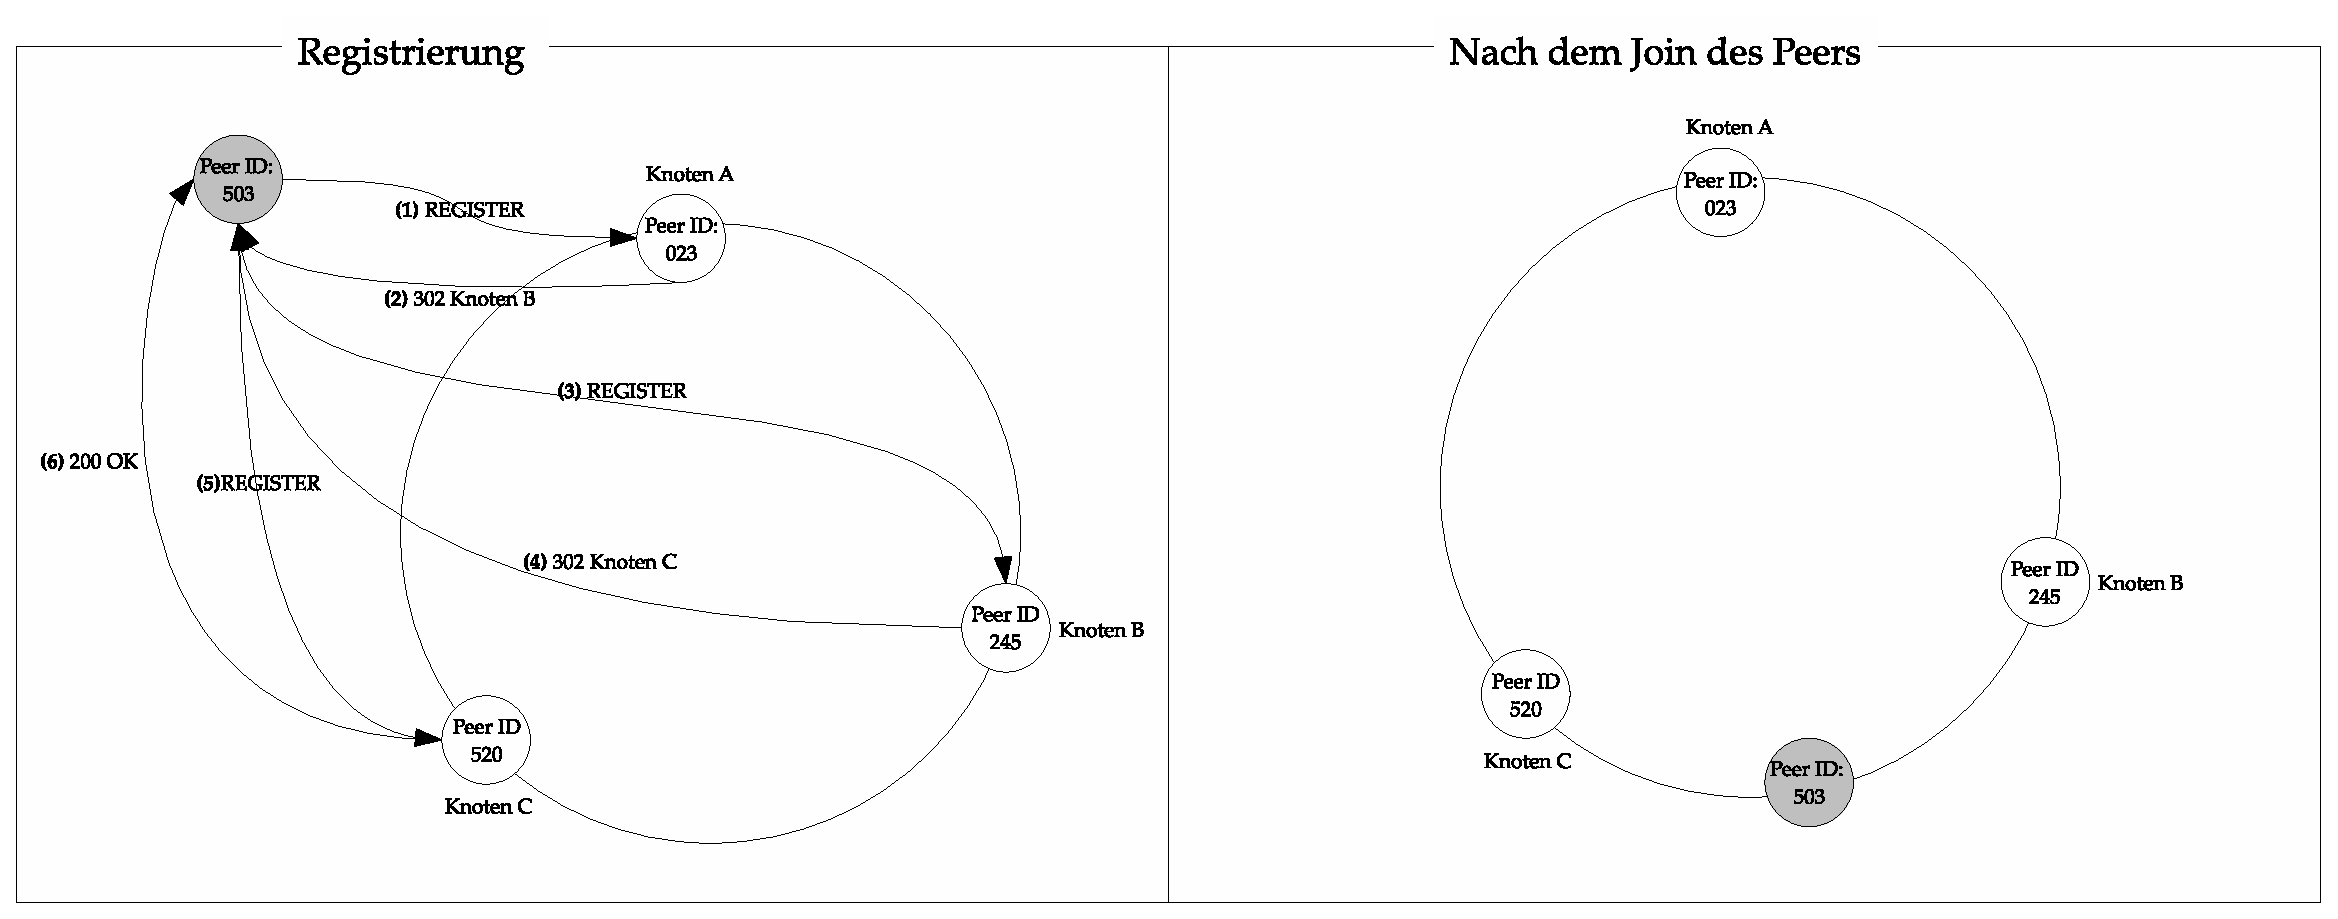
\includegraphics[width=1.00\textwidth]{grafiken/p2psipregisterandjoin.eps}
	\caption{Registrierung eines neuen Knotens bei Knoten C}
	\label{fig:p2psipregisterandjoin}
\end{figure}

\begin{figure}[tbh]
	\centering
		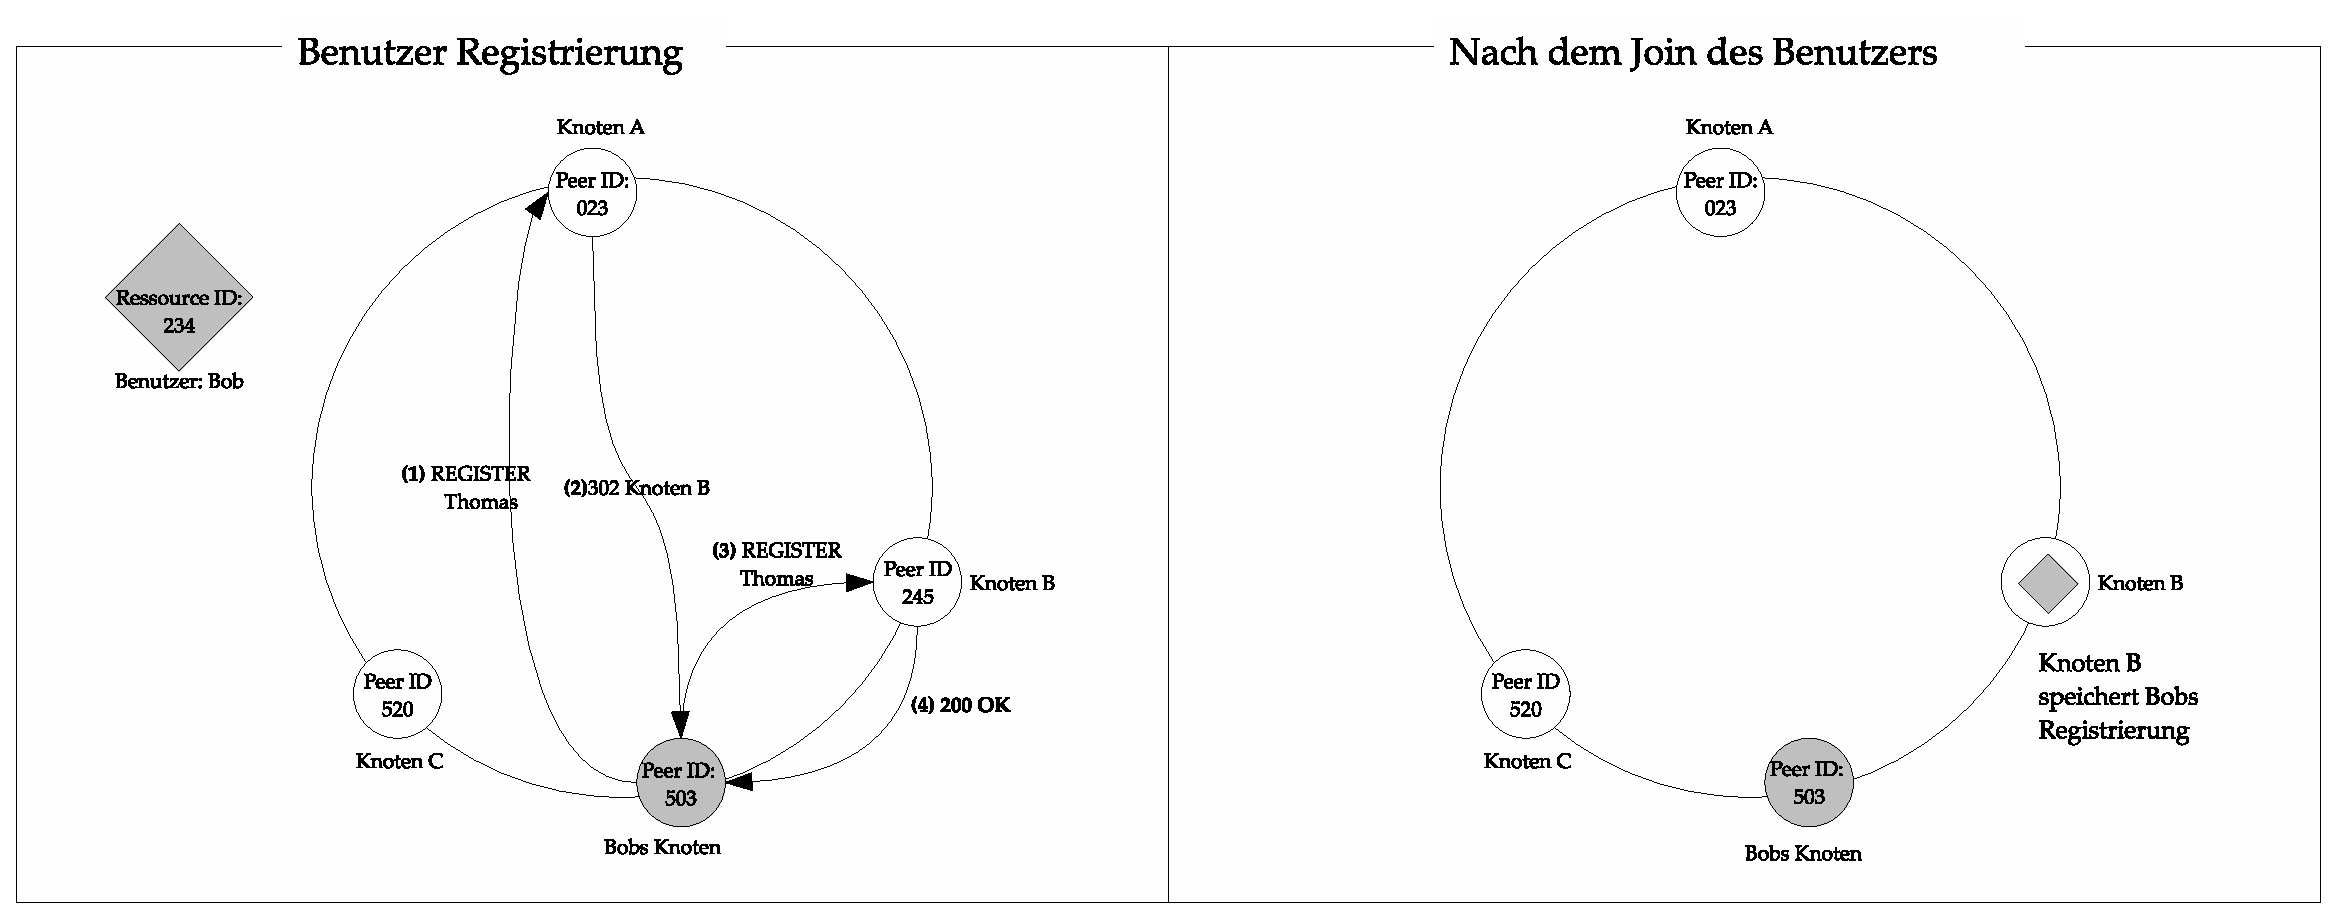
\includegraphics[width=1.00\textwidth]{grafiken/p2psipregisterandjoin_user.eps}
		\caption{Registrierung des Benutzers}
	\label{fig:p2psipregisterandjoin_user}
\end{figure}

\subsubsection{Aufbau einer Verbindung}
M�chte ein Benutzer nun einen anderen Benutzer kontaktieren, so wird eine Suchanfrage an das Overlay gestellt, die den \textit{Hash} der \textit{Ressourcen-ID} beinhaltet. Diese wird so lange durch das Netz geleitet, bis der Knoten gefunden wird, der die entsprechende IP-Adresse enth�lt. Dieser Knoten beantwortet die Anfrage und der Benutzer kann nun direkt mit dem Zielknoten kommunizieren (siehe Abbildung \ref{p2psipcall}).

Verlassen Knoten das Overlay, so m�ssen sie ihre Information an andere Knoten weitergeben. Oft wird auch die Information mehrfach repliziert, um Datenverlust zu vermeiden. 

\begin{figure}[tbh]
	\centering
		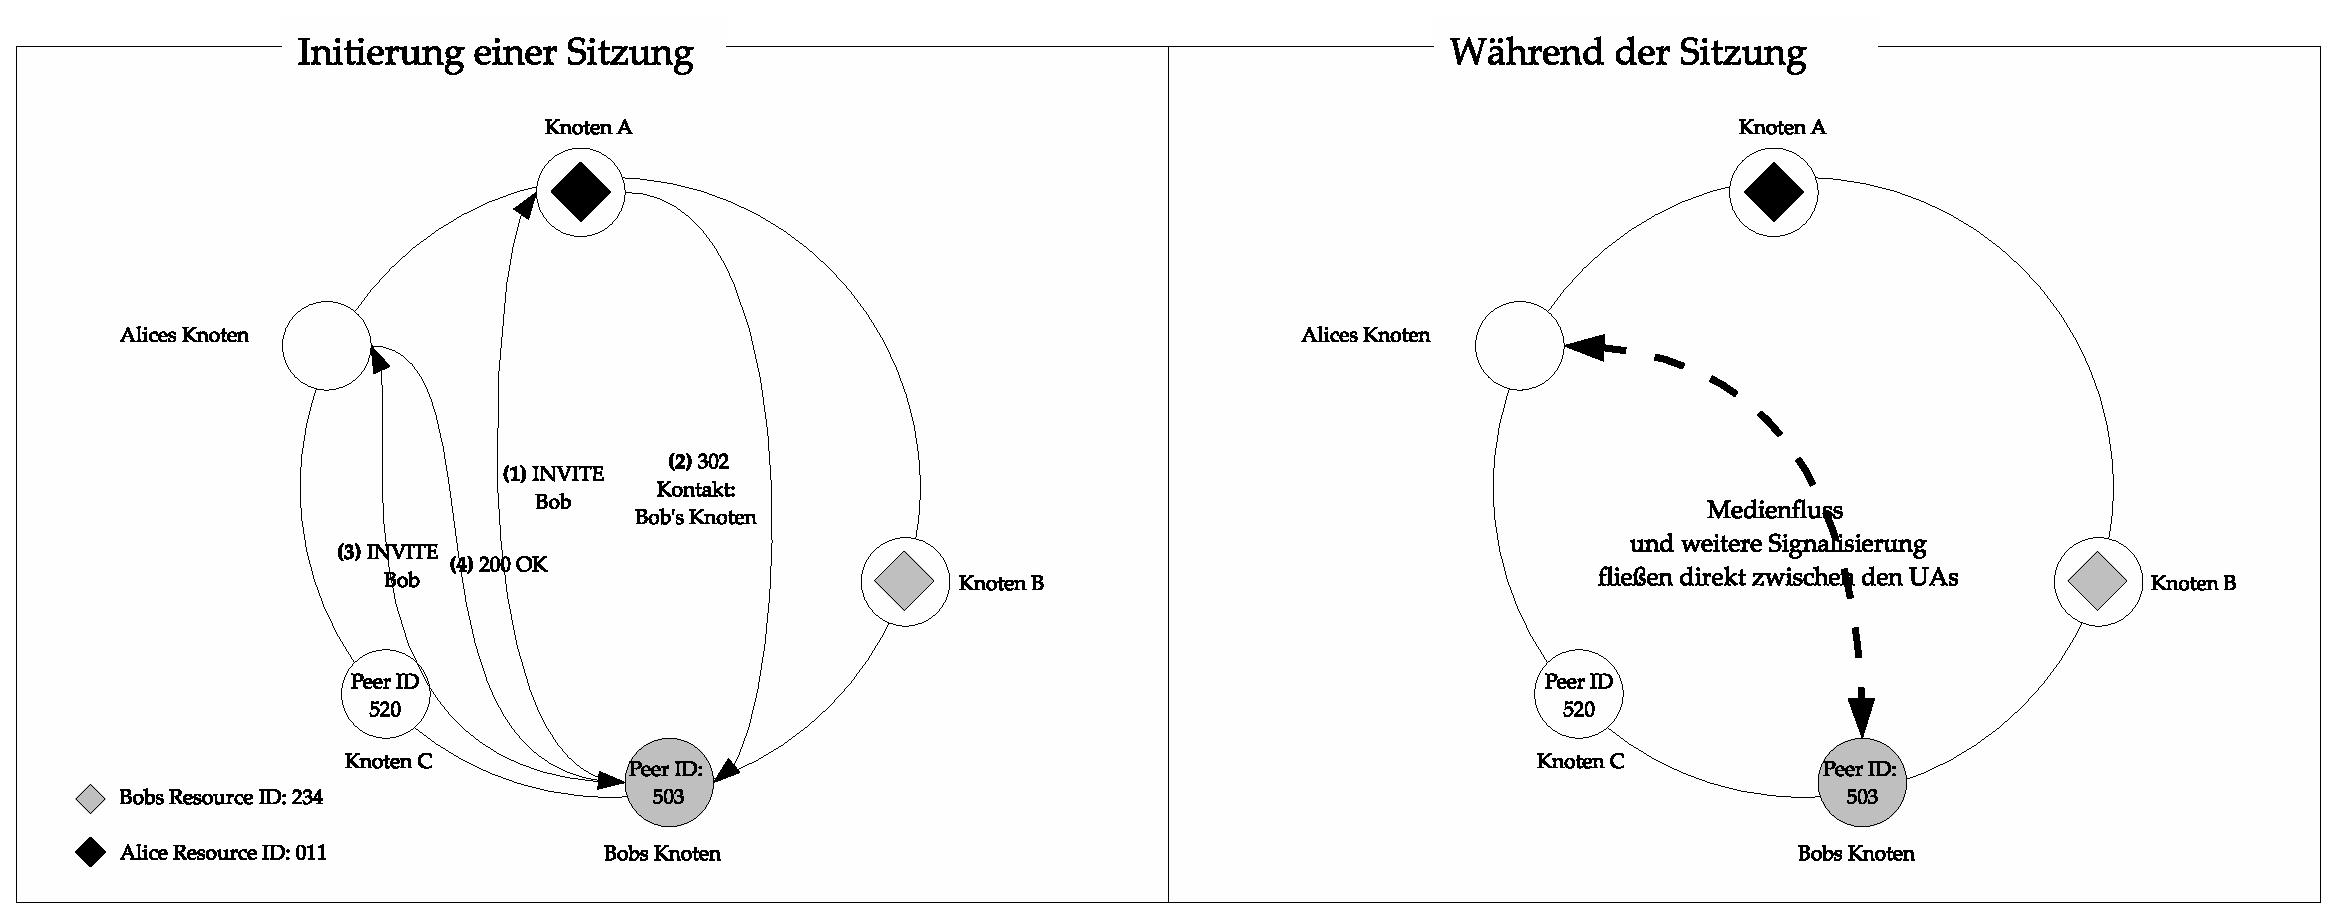
\includegraphics[width=1.00\textwidth]{grafiken/p2psipcall.eps}
	\caption{Ein schematischer Ablauf eines Anrufs bei P2P-SIP}
	\label{fig:p2psipcall}
\end{figure}

Bryan, Lowekamp und Jennings schlagen im SOSIMPLE-Prototyp \cite{bryan05s} eine Kombination vom SIP- und-SIMPLE Protokoll vor, in dem Knoten in einem Chord-basierten DHT Overlay verwaltet werden. Alle Nachrichten, die ben�tigt werden um das DHT aufrecht zu erhalten, Benutzer zu registrieren, Ressourcen zu lokalisieren, Sitzungen zu verwalten sind reine SIP-Nachrichten. Da SIP als generisches Protokoll entworfen wurde, m�ssen nur die Nachrichtentypen um zus�tzliche Header erg�nzt werden. Ein �hnliches Konzept f�r SIP-Telefonie auf Basis eines Chord-basierten-DHT, schlagen auch Singh und Schulzrinne vor \cite{schulzrinne05}.

\subsection{Einsatz von P2P-SIP f�r Spiele}
P2P-SIP l�sst sich auch f�r Spiele einsetzen und ist vor allem deswegen interessant, da es Vorteile von strukturierten Peer-to-Peer-Ans�tzen mit der hohen Abstraktion von SIP kombiniert. Die vorgestellten Ans�tze f�r P2P-Spiele k�nnten eine solche Netzwerkschicht nutzen, um eine standardisierte Umsetzung zu gew�hrleisten. Man kann sogar noch weiter gehen und sagen, dass ein funktionierendes P2P-SIP bereits ausreicht, um als Basis f�r P2P-Spiele zu dienen. Prinzipiell sind in einem SIP-Standard alle Komponenten vorhanden, die man f�r eine P2P-Architektur braucht und �bliche Probleme wie das NAT-Traversal bereits erfolgreich gel�st. Da die VoIP-Technologie �hnliche Konzepte und Probleme wie im Spielebereich aufweist, sind wichtige Komponenten bereits in Form von Lokationsdiensten, Pr�senzdiensten, Proxys, Registraren oder STUN-Servern abstrahiert worden. P2P Ans�tzen Spielebereich steht diese Entwicklung noch bevor. 

Zum Beispiel k�nnte der implementierte Client-Server Ansatz mit wenigen Ver�nderungen in einer P2P-SIP-Architektur eingesetzt werden.  Man k�nnte so auf der Abstraktionsebene zwar das bew�hrte Konzept einer Client-Server Anordnung beibehalten, obwohl die tats�chliche Architektur bereits komplett dezentralisert wurde. Der Ansatz zentrale Komponenten eines hybriden Systems dezentral zu realisieren wird bereits im BitTorrent-Protokoll erfolgreich umgesetzt.

Indem man eine Unterscheidung zul�sst auf welche Knoten der Lokationsdienst verteilt wird, k�nnen Supernodes Konzepte oder Serverfarmen helfen den Dienst performanter und ausfallsicherer zu machen.

\subsection{Architektur Variationen}
Es bestehen drei alternative Architektur Variationen beim Einsatz mit DHT zur Verf�gung. 

Der DHT kann auf eine dedizierte Server Farm limitiert werden. F�r die Registrierung verbinden die Teilnehmer sich zu einem der Server. Wie bereits geschildert implementieren die Server selbst eine skalierbare Datenstruktur wie DHT, um den entsprechenden Eintrag zu finden. Der Teilnehmer muss jedoch mindestens einen Server finden und zu ihm verbinden. Diese Option beinhaltet keine Modifizierung der Clients, bietet aber eine zuverl�ssige Server Farm Architektur. 

%\begin{figure}
%	\centering
%		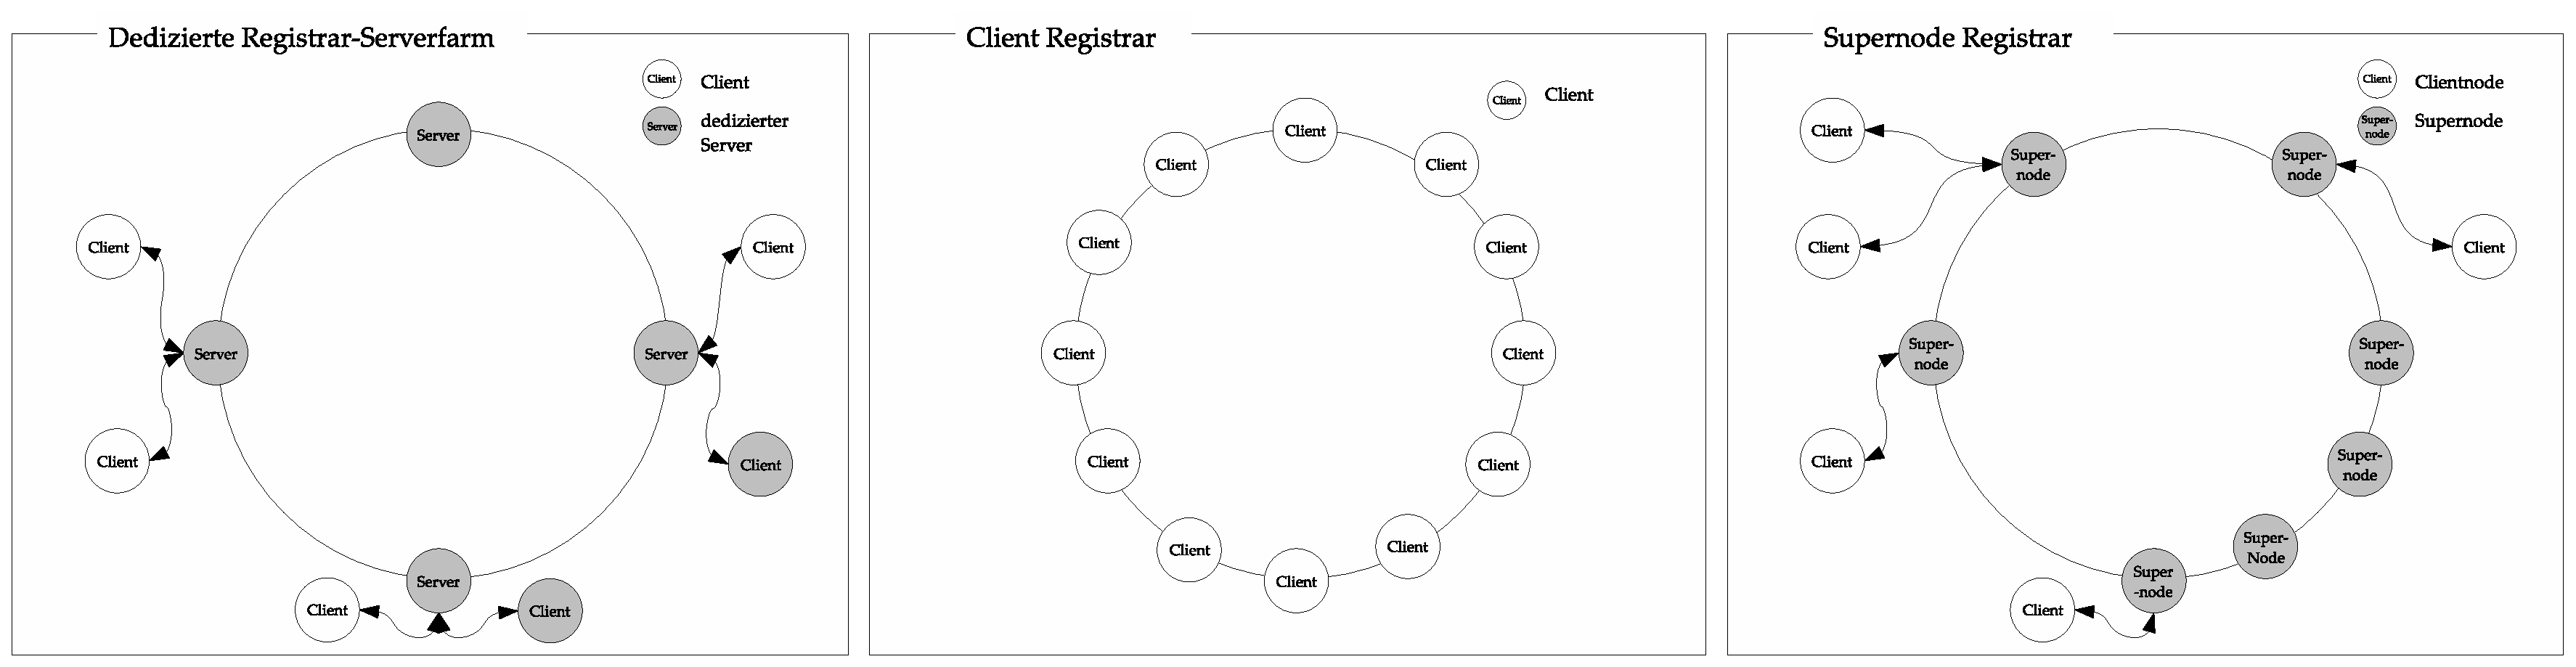
\includegraphics[width=1.00\textwidth]{grafiken/3in1registrar.eps}
%	\caption{Verschiede Registrar Variationen}
%	\label{fig:3in1registrar}
%\end{figure}

%\begin{figure}[tbh]
%	\centering
%		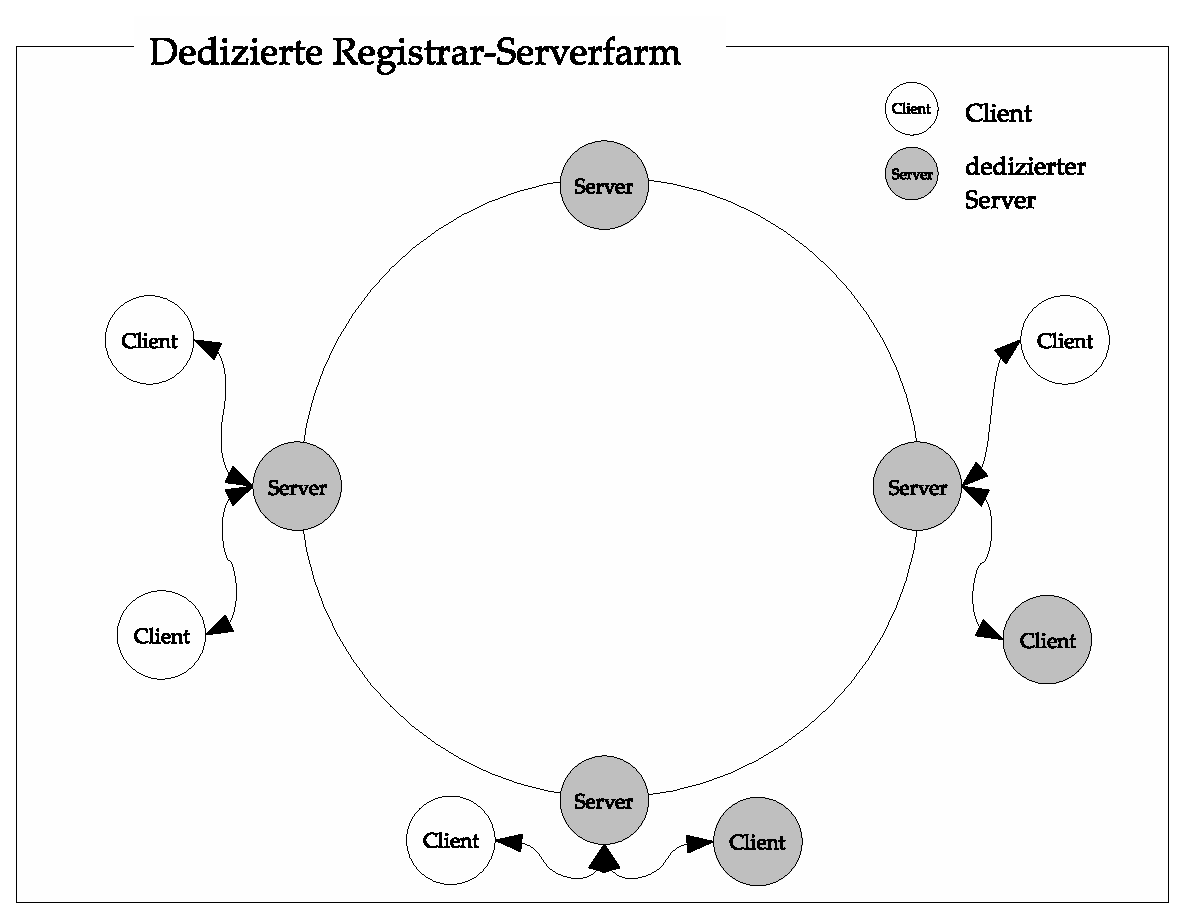
\includegraphics[width=0.60\textwidth]{grafiken/registrar-dediziert.eps}
%	\caption{Ein Registrar wurde auf dedizierte Server verteilt}
%	\label{fig:registrar-dediziert}
%\end{figure}

Eine andere M�glichkeit besteht darin, dass jeder Client auch als Server arbeitet. Das Problem hierbei ist, dass nicht alle Knoten eine gleiche Verf�gbarkeit und Bandbreiten Kapazit�t besitzen. Ein Knoten mit geringer Bandbreite und einer schlechten Anbindung z.B. hinter einer NAT besitzt eventuell nicht ausreichende Ressourcen um im DHT funktionieren. 

%\begin{figure}[tbh]
	%\centering
	%	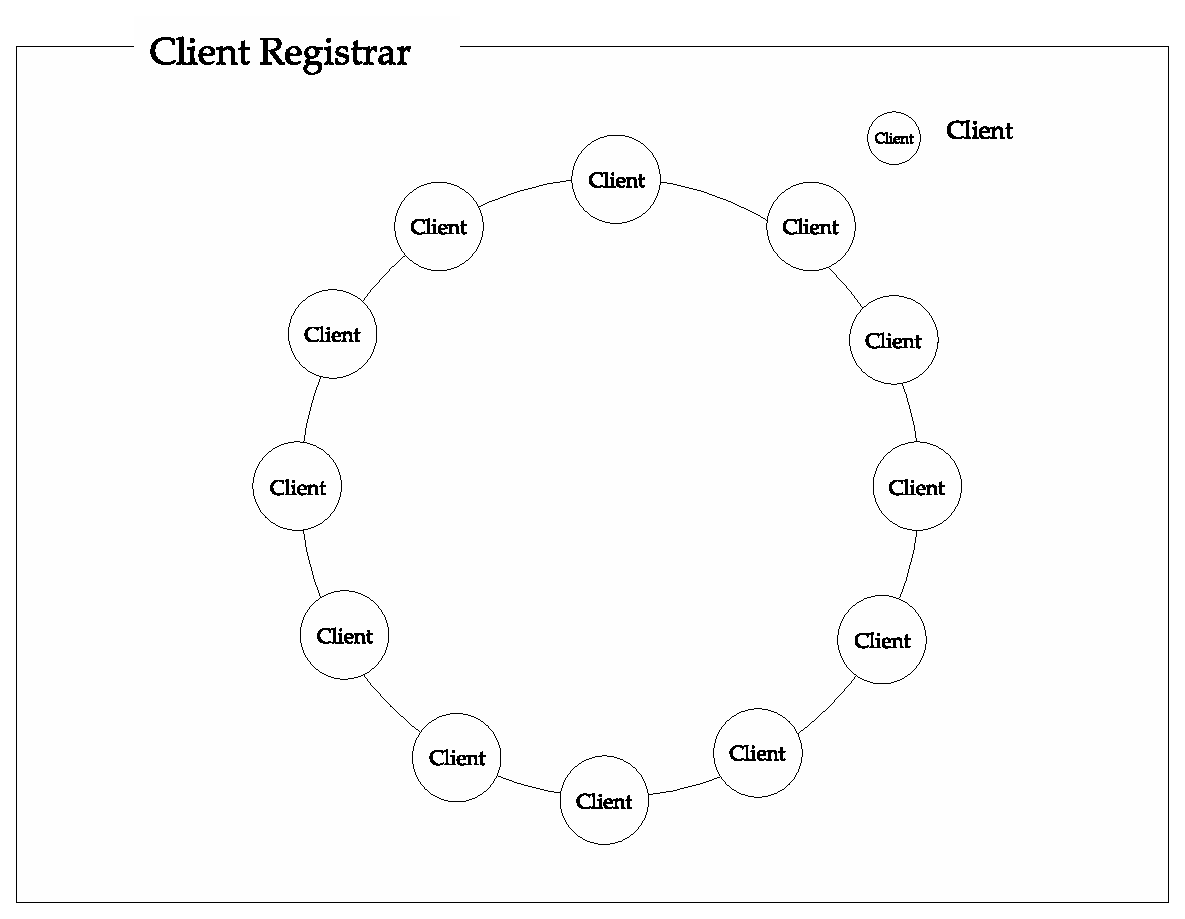
\includegraphics[width=0.60\textwidth]{grafiken/registrar-client.eps}
	%\caption{Ein Registrar wird zwischen allen Teilnehmern verteilt}
	%\label{fig:registrar-client}
%\end{figure}

Im dritten Ansatz kann eine Mischung aus den zwei Ans�tzen gew�hlt werden, in der Knoten mit hoher Kapazit�t  (Bandbreite, CPU, Speicher) und Verf�gbarkeit (�ffentlich erreichbar) zu \textit{SuperPeers} ernannt werden. Solche Peers k�nnen f�r die Registrierung von anderen Teilnehmern genutzt werden. Dabei entscheidet jeder Knoten aufgrund seiner Eigenschaften selbst ob ein SuperPeer werden will oder nicht.

%\begin{figure}[tbh]
%	\centering
%		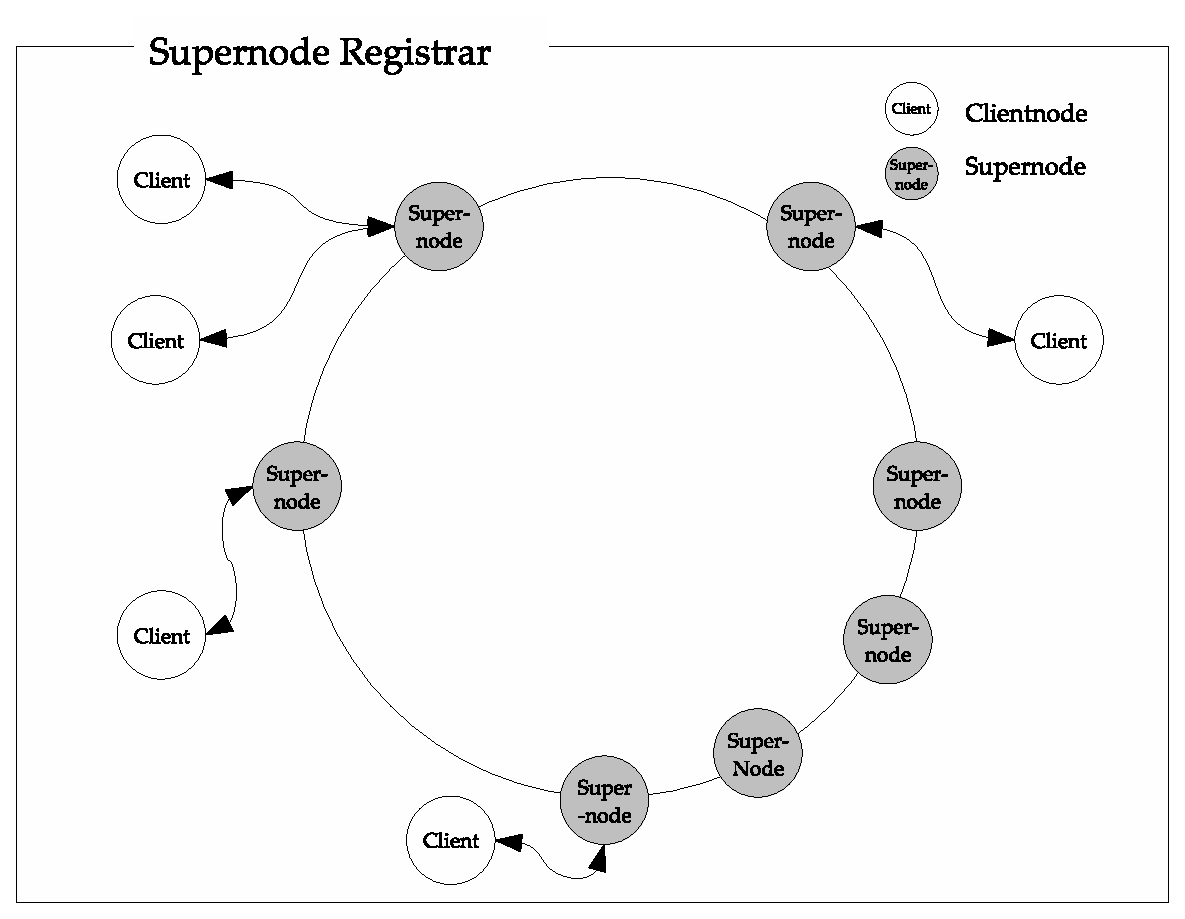
\includegraphics[width=0.60\textwidth]{grafiken/registrar-supernode.eps}
%	\caption{Ein Registrar wird nur zwischen Teilnehmern mit hoher Kapazit�t  (Bandbreite, CPU, Speicher) verteilt}
%	\label{fig:registrar-supernode}
%\end{figure}
\newpage~
\chapter{Evaluation}

In diesem Kapitel wird das Resultat der Umsetzung mit konkreten Messergebnissen erfasst. Anhand eines Szenarios wird der Full-Mesh-Ansatz mit dem entwickelten Partial-Mesh-Ansatz verglichen und es werden dabei Einsparungen der Bandbreite aufgezeigt. In einem weiteren Szenario wird der Bandbreitenverbrauch des Prototyps in den in Kapitel 7 vorgestellten Zonen gemessen. Dabei werden jeweils Messungen f�r die Audiocodec-Variationen, die SIP-Hold- und die  RTP-Silence-Suppression-Technik vorgenommen. Au�erdem werden die Tauglichkeit von SIP als Netzwerkschnitstelle anhand von Roudtrip-Time-Messungen, sowie die Grenzen der Conference Bridge beim Mischen von Audiosignalen aufgezeigt. 

\section{Versuchsaufbau}

Um �nderungen des Bandbreitenverbrauchs zu messen, wurden alle versendeten und empfangenen Pakete auf einem Spiel initiierenden Rechner protokolliert\footnote{Gerald Combs: Wireshark 1.0.0, Seite besucht 08.05.2008, http://www.wireshark.org/} und ausgewertet. Danach wurden die Daten nach den Quell-IP-Adressen gefiltert, um so den Bandbreitenverbrauch den jeweiligen Teilnehmern zuzuordnen. Um den reinen Bandbreitenverbrauch der Audioverbindungen zu messen, wurden auch Pakete, die Positions�nderungen der Teilnehmer untereinander broadcasten ausgefiltert. F�r alle Messungen wurde die Testumgebung aus Abschnitt \ref{testumgebung} eingesetzt. 

Die virtuellen Zonenradien betrugen 600 Pixel f�r die private Zone, 1200 Pixel f�r die soziale Zone und 2400 Pixel f�r die �ffentliche Zone. Die Gesamtgr��e des Spielfeldes betrug $5000 \cdot 5000$ Pixel und die H�he und Breite eines Avatars $300 \cdot 100$ Pixel. 

\subsubsection{Header-Overhead}
Bei fast\footnote{In Abschnitt \ref{audiocodec-zonen} wurde der Speex-Codec mit einer Abtastrate von 8kHz eingesetzt.} allen Messungen wurde der Speex Codec mit einer Abtastrate von 16kHz benutzt, der eine mittlere Bitrate von 16.8 Kbit/s\footnote{Speex Codec Quality Comparison (Xiph OSC) , Seite besucht 22.03.2008, http://speex.org/comparison/} besitzt.  Die Stimm-Abtastrate lag bei 20ms.

Obwohl der Audiocodec eine Bitrate von 16.8 Kbit/s besitzt, weist die tat\-s�chlich verbrauchte Bandbreite jedes Rechners einen Upload von 5 KByte/s oder 40 Kbit/s auf, wie man in allen Messungen erkennen kann. Die Differenz zwischen der Nutzlast (Payload) und der tats�chlichen Bandbreite liegt im Header-Overhead. 

F�r die Header werden pro Paket insgesamt 40 Bytes ben�tigt (IP\footnote{RFC: Internet Protocol, Seite besucht 22.03.2008, http://www.ietf.org/rfc/rfc791.txt}: 20 Bytes, UDP\footnote{RFC: User Datagram Protocol, Seite besucht 22.03.2008, www.ietf.org/rfc/rfc768.html} : 8 Bytes, RTP\footnote{siehe Abschnitt \ref{rtp-header}} : 12 Bytes). Zus�tzlich dazu kommen 20 Bytes VPN-Headerinformationen\footnote{VPN Protocols, Seite besucht 22.03.2008, http://www.vpnc.org/vpn-standards.html}, da der Laptop, der die Messung ausf�hrte durch einen VPN mit dem Uni-Netz verbunden war. 

Geht man davon aus, dass jedes Paket ein Stimm-Sample �bertr�gt und diese alle 20ms abgetastet werden, ergeben sich 50 Pakete pro Sekunde. Jedes Paket beinhaltet einen VPN/IP/UDP/RTP-Header von 480 Bit (60 Byte*8). Also werden pro Sekunde 24.000 Bit (480 Bit * 50) Headerinformationen verschickt. Dies ist genau die Differenz zwischen der Bitrate des Audiocodecs und der tats�chlich verbrauchten Bandbreite.

\subsubsection{Aktive Silence-Suppression}

In allen Messergebnissen ist auch zu erkennen, dass die Bandbreite in der sozialen und privaten Zone einer gewissen Varianz von bis zu 5 KByte/s unterliegt. Diese ist auf die aktive Silence-Suppression in der privaten und sozialen Zone zur�ckzuf�hren, die durchgef�hrt wird, wenn das Audiosignal einen bestimmten Schwellenwert unterschreitet. Sie wird automatisch von PjSIP und dem \textit{Preprocessor} des Speex Audiocodecs durchgef�hrt. Da die verwendeten  Mikrofone sich hardwarebedingt in ihrer Empfindlichkeit unterscheiden, verhalten sich beide Kurven nicht immer exakt gleich.

\section{Full-Mesh- vs. Partial-Mesh-Szenario}

Um zu verdeutlichen, wie der umgesetzte Ansatz zu Einsparungen beim Verbrauch der Bandbreite eingesetzt werden kann, wird er mit einem gew�hnlichen Full-Mesh-Ansatz verglichen, in dem jeder Teilnehmer des Spiels mit allen anderen 
Teilnehmern Audioverbindungen aufbaut, unabh�ngig davon, wo sich diese im Spiel befinden.

Im vorgeschlagenen Partial-Mesh-Ansatz dagegen verbindet sich der Teilnehmer nur mit Spielern, die sich in seiner unmittelbaren N�he befinden. Dieses Verhalten entspricht dem umgesetzten Proximit�tskonzept, in dem nur Audioverbindungen mit Spielern aufgebaut werden, die sich mindestens in der �ffentlichen Zone befinden.

In einem einfachen Szenario werden beide Ans�tze ausprobiert: Hier betreten 5 Spieler nacheinander die Spielewelt. Die Nummer des Teilnehmers entspricht der Reihenfolge seiner Teilnahme am Spiel: Zun�chst betritt Teilnehmer 1 das Spielfeld, danach Teilnehmer 2 usw... .Spieler 1, 2 und 3 befinden sich in gegenseitiger H�rn�he, w�hrend Spieler 4 und 5 isolierte Positionen einnehmen. Da der Versuch mehrmals manuell ausgef�hrt wurde, sind die Beitrittszeitpunkte der Teilnehmer nicht exakt uniform verteilt, was jedoch die Aussagen der Versuchsergebnisse nicht beeinflusst. 

\begin {figure}[ht]
\begin{center}
\subfloat[Full-Mesh-Ansatz\label{fig:fullmesh}]{

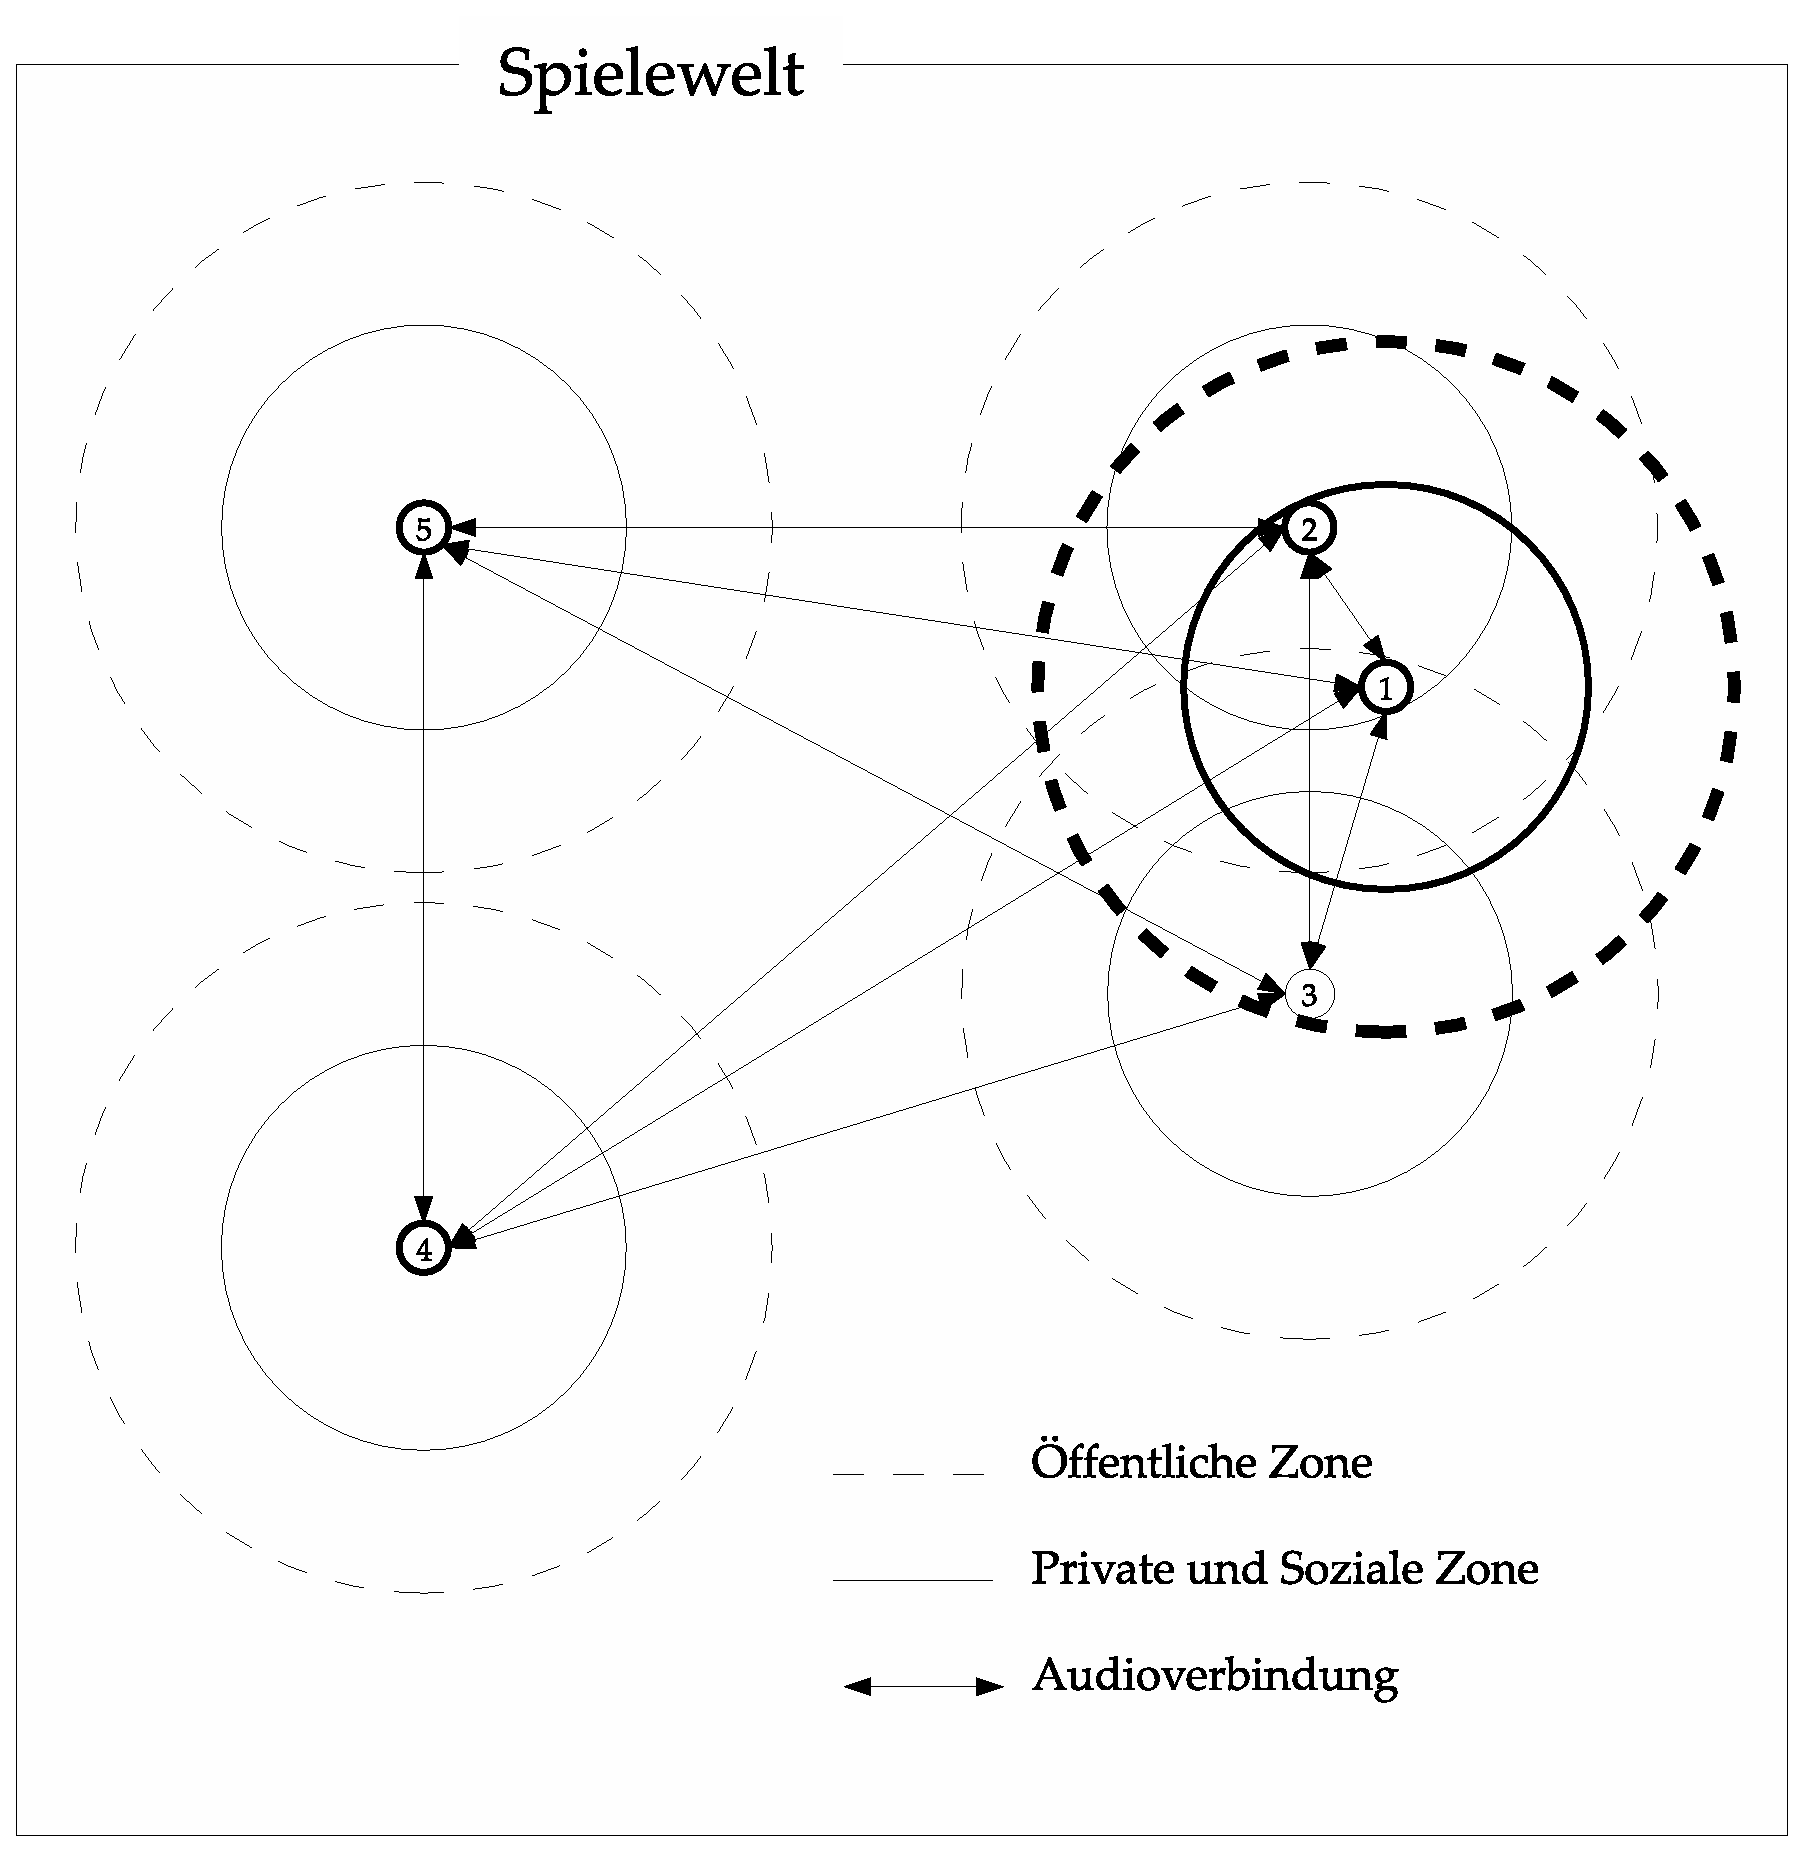
\includegraphics[width=.5\textwidth]{grafiken/fullmesh.eps}
}
\subfloat[Partial-Mesh-Ansatz\label{fig:partialmesh}]{

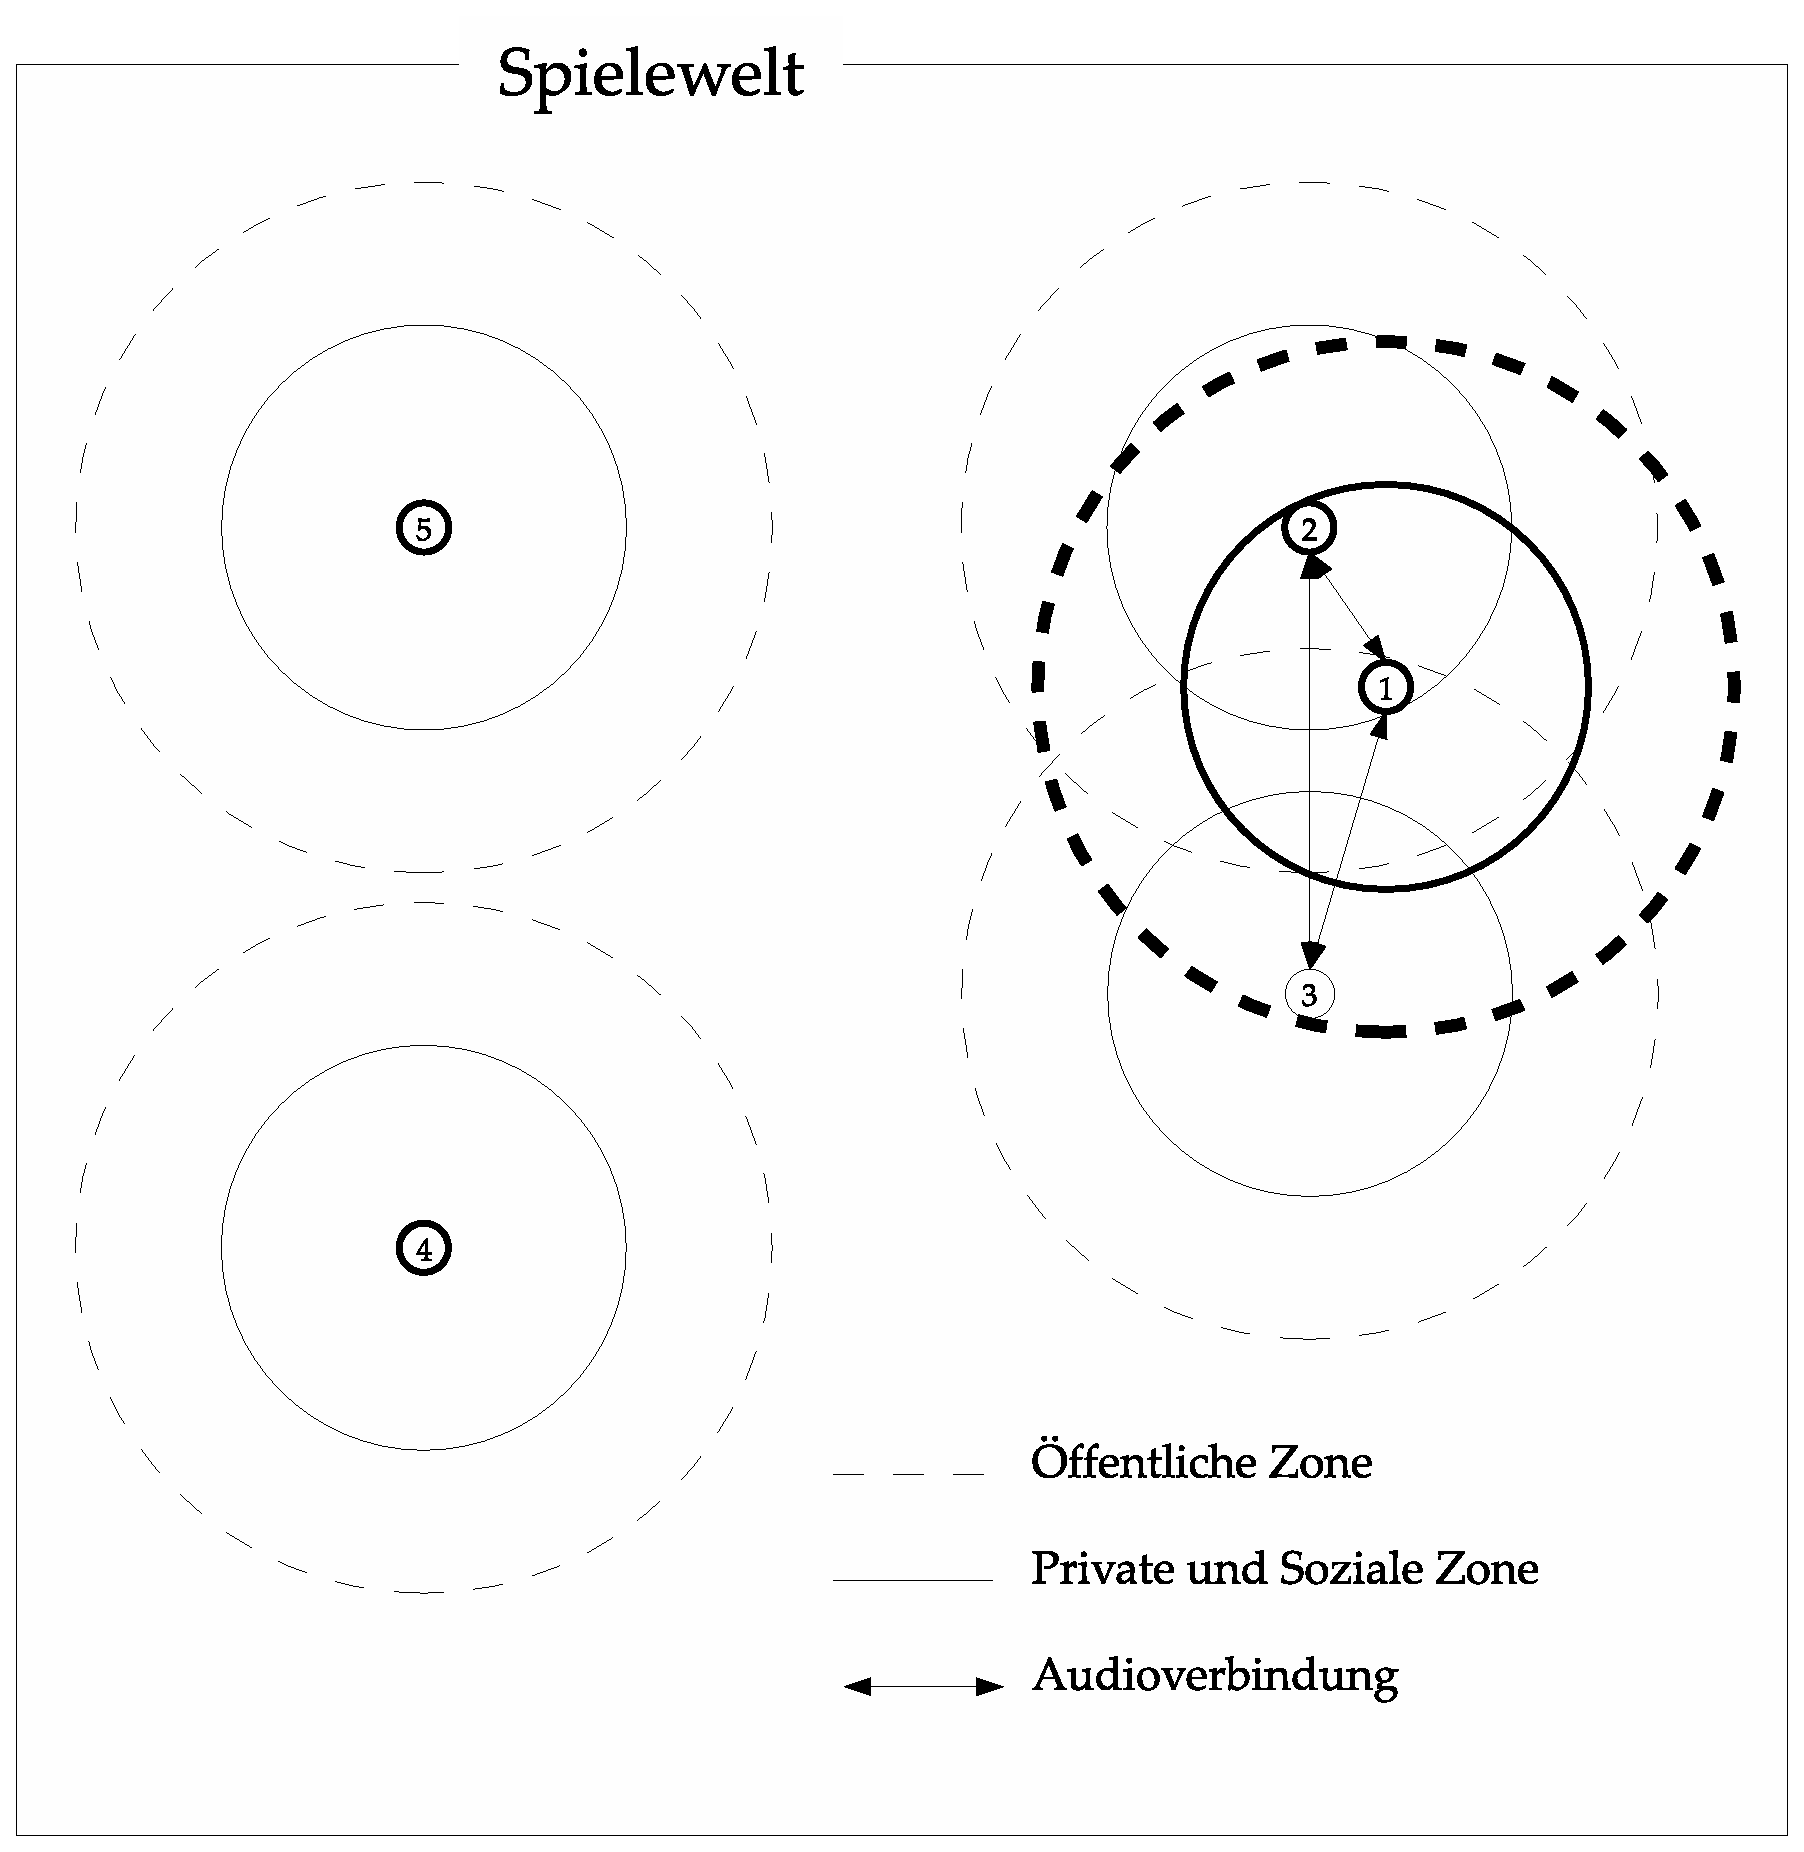
\includegraphics[width=.5\textwidth]{grafiken/partialmesh.eps}
}
\caption {Szenario zum Vergleich der Anzahl etablierter Audioverbindungen}
\label{szenario}
\end{center}
\end{figure}

\subsection{Full-Mesh}
Die Szenario-Abbildung \ref{fig:fullmesh} zeigt, dass beim Full-Mesh-Ansatz jeder Teilnehmer Verbindungen zu allen anderen Teilnehmern etabliert und so ein Full-Mesh zwischen allen Teilnehmern gebildet wird. 

%\begin{figure}[tbh]
%	\centering
%		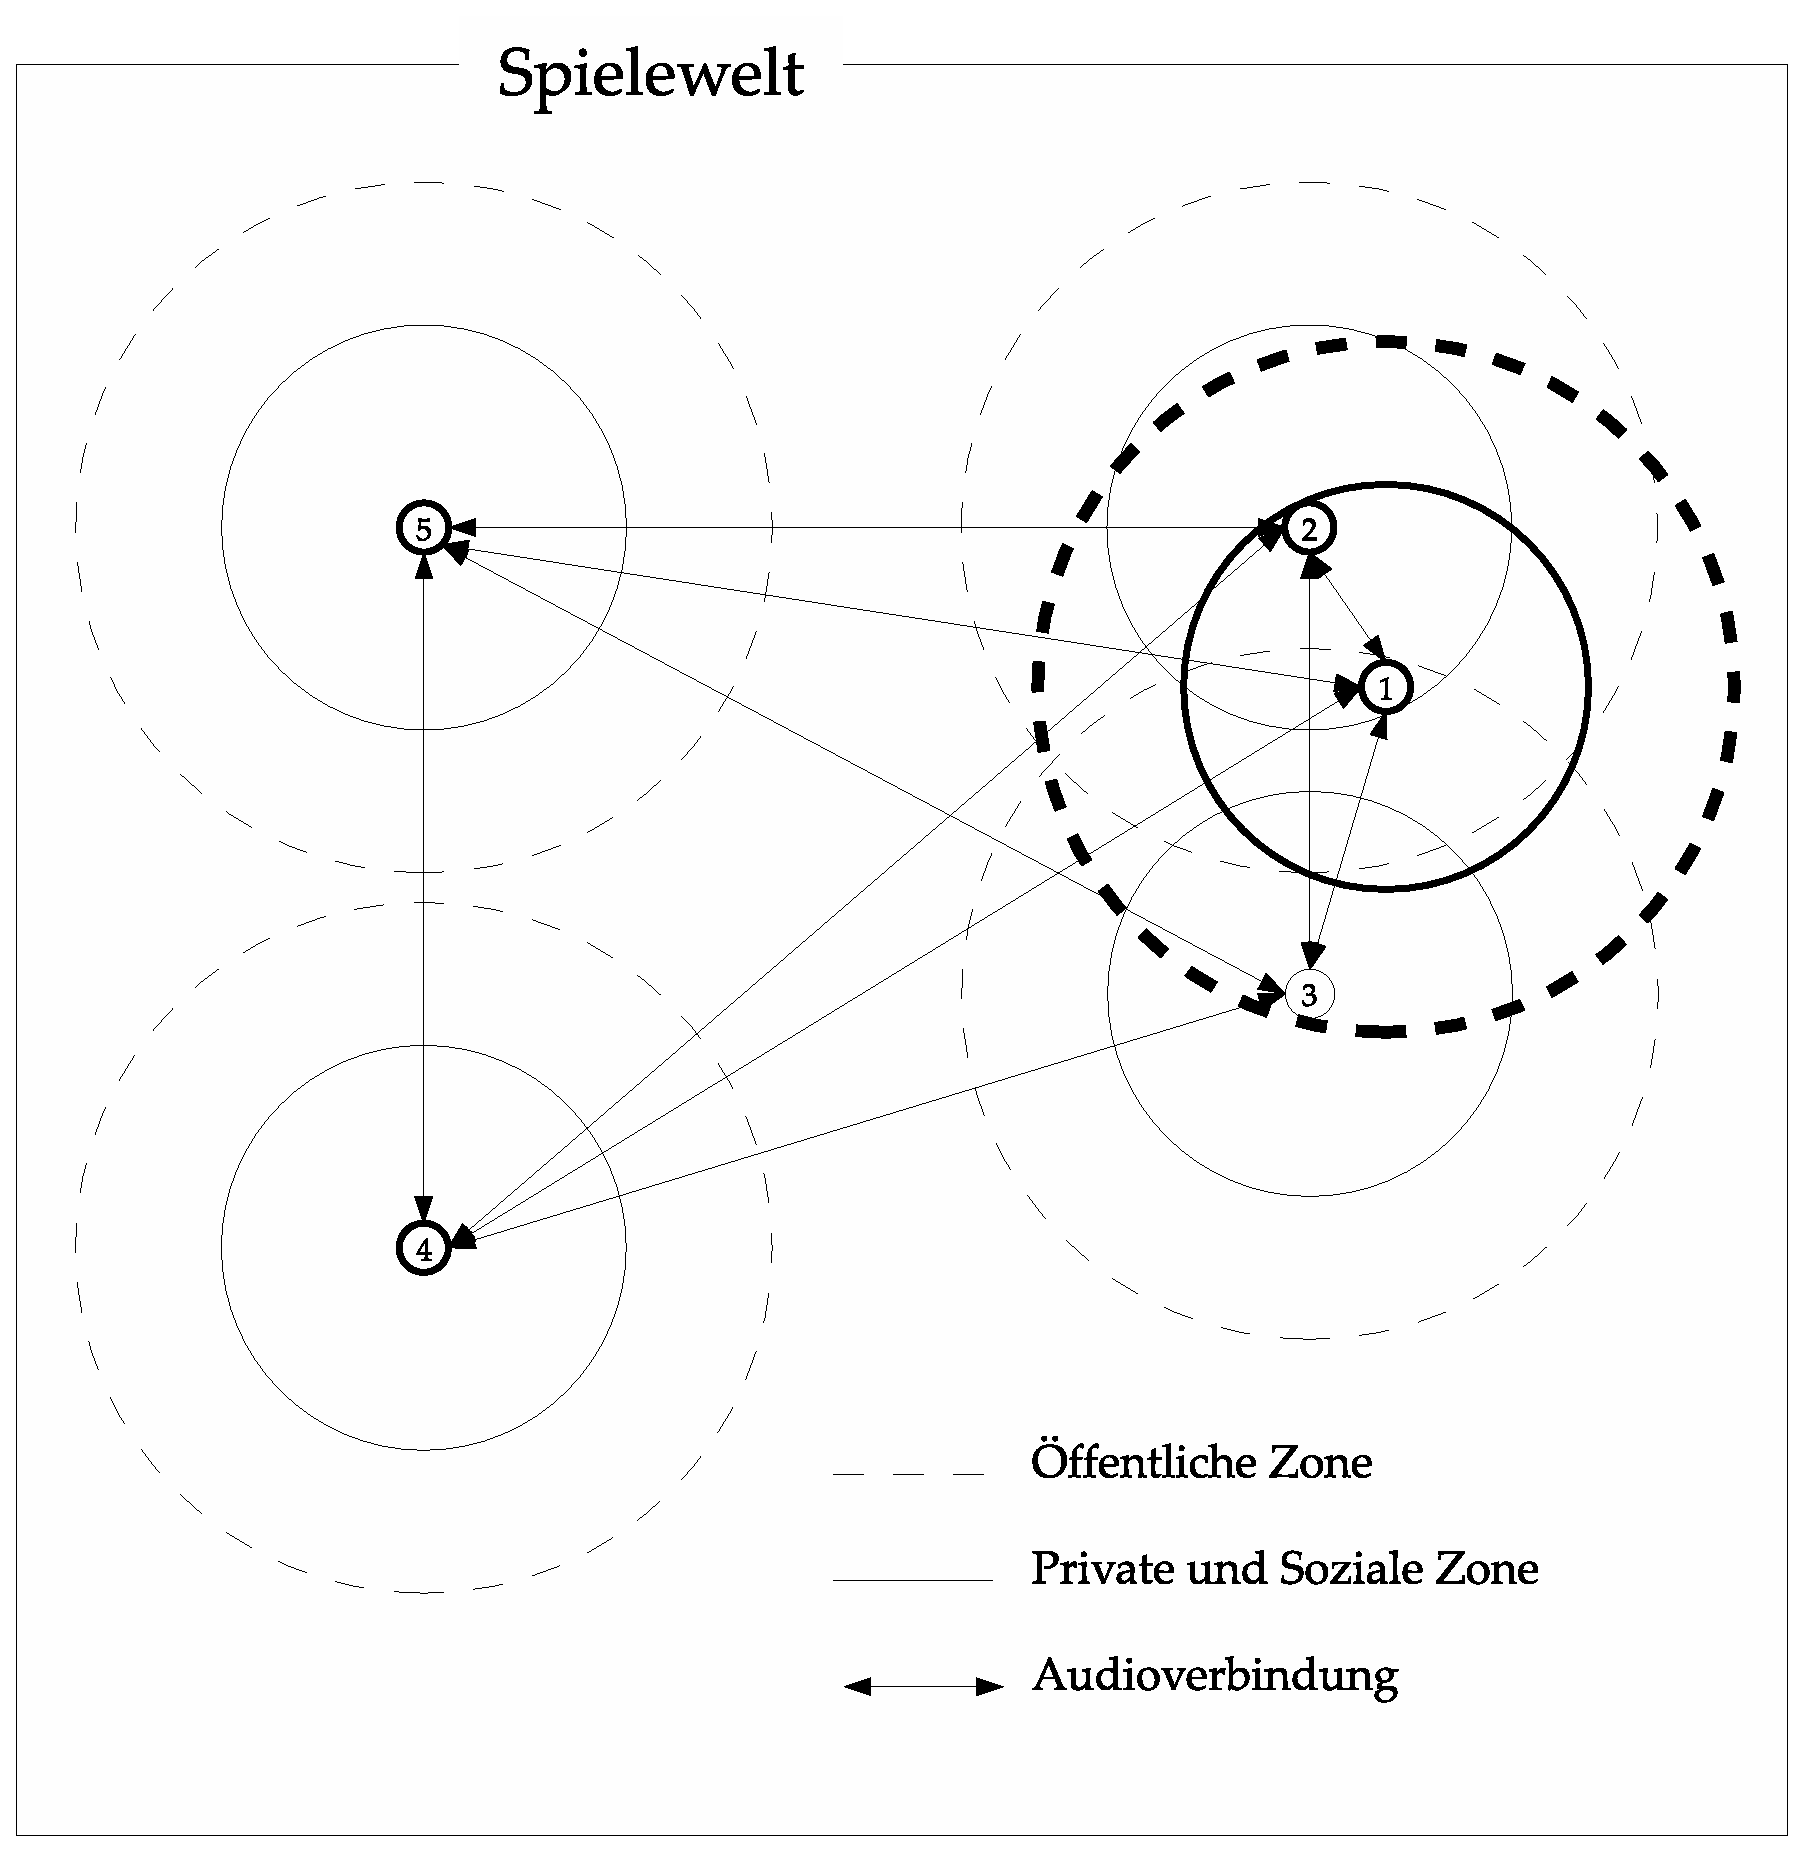
\includegraphics[width=.70\textwidth]{grafiken/fullmesh.eps}
%			\caption{Audioverbindungen im Full-Mesh-Ansatz}
%	\label{fig:fullmesh}
%\end{figure}

Abbildung \ref{fig:fullmesh-withchart} zeigt den Bandbreitenverbrauch von Teilnehmer 1 in Abh�ngig\-keit zur Anzahl der sich im Spiel befindlichen Spielern. Da alle 10 Sekunden ein weiterer Spieler das Spielfeld betritt, wird auch eine Audioverbindung mit diesem Spieler aufgebaut. Dadurch wird der Verbrauch der Bandbreite jeweils um weitere 10kByte/s (5 KByte Up-/ 5 KByte Download) erh�ht. Dieses Vorgehen f�hrt bei bereits 5 anwesenden Teilnehmern zu einem Gesamtbandbreitenverbrauch zwischen Teilnehmer 1 und den Teilnehmern 2,3,4,5 von �ber 40 KByte/s. Im Full-Mesh flie�t zum Zeitpunkt $t4$ zwischen allen Teilnehmern bereits ein Gesamtaudiostrom von 100 kByte/s ($10 \cdot 10kByte/s$).

\begin{figure}[tbh]
	\centering
		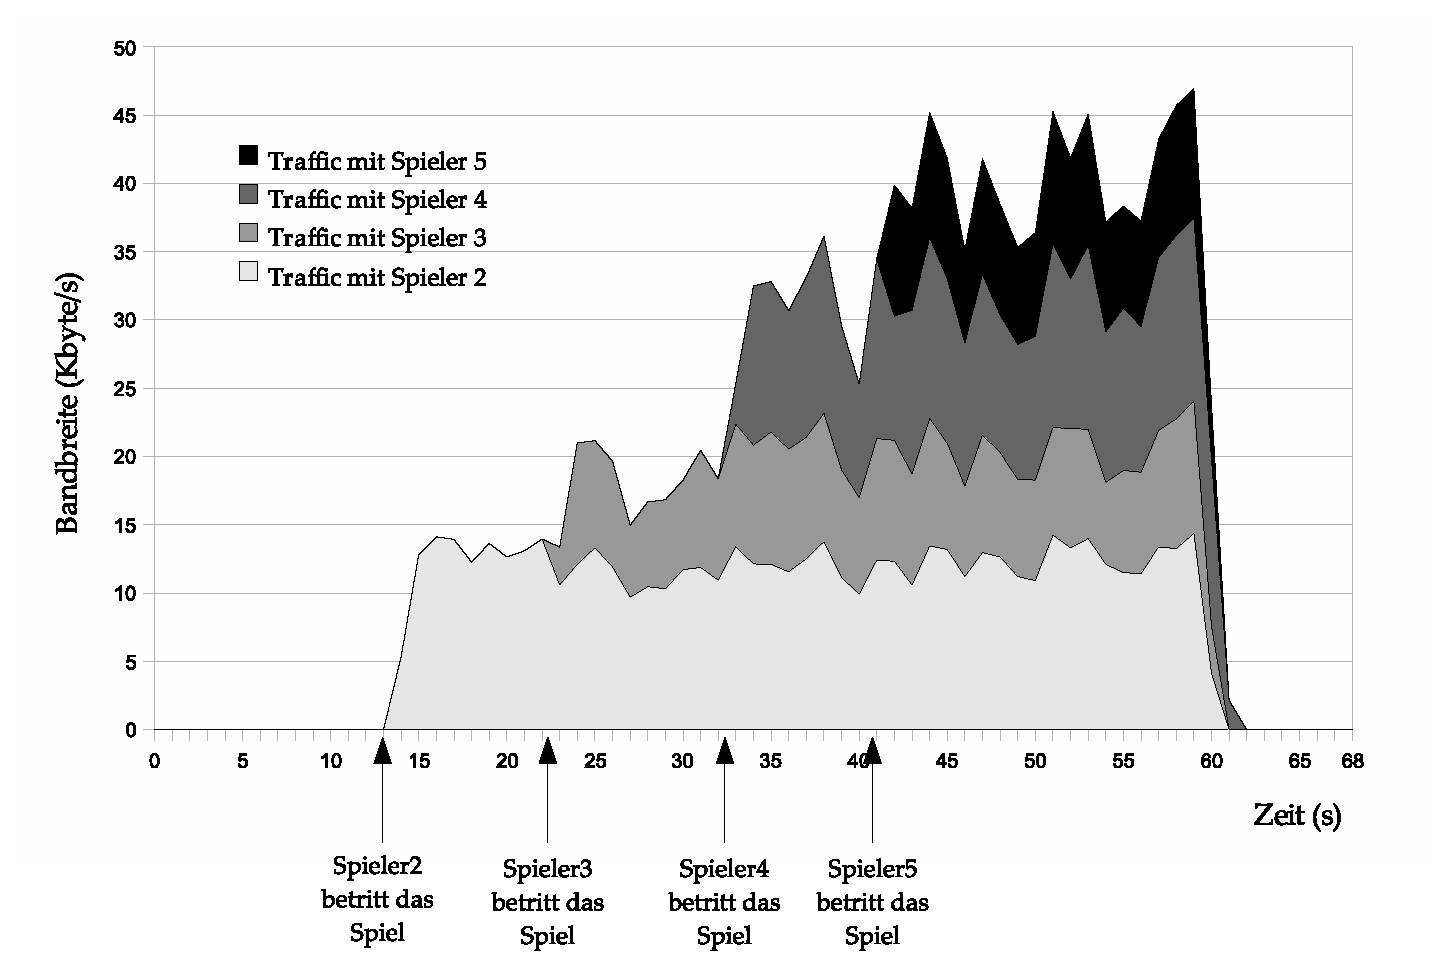
\includegraphics[width=\textwidth]{grafiken/fullmeshchart.eps}
	\caption{Bandbreitenverbrauch beim Full-Mesh-Ansatz}
	\label{fig:fullmesh-withchart}
\end{figure}

\subsection{Partial-Mesh}
Im gleichen Szenario wurde nun die Partial-Mesh-Technik eingesetzt, bei der nur noch Verbindungen mit Teilnehmern aufgebaut wurden, die sich mindestens in der �ffentlichen Zone des Spielers befinden (siehe Abbildung \ref{fig:partialmesh}).

Entsprechend dem Zonenkonzept wird in der �ffentlichen Zone zun�chst ein SIP-Anruf ausgef�hrt, jedoch gleichzeitig eine Silence-Suppression auf RTP-Ebene vorgenommen. Diese wird so lange aufrecht erhalten, bis der Teilnehmer sich in die soziale Zone begibt. In der sozialen Zone wird der volle RTP-Audiostrom zwischen den Teilnehmern initiiert. 

Wie man in der Szenario-Abbildung \ref{fig:partialmesh} erkennen kann, f�hrt diese Regel dazu, dass mit Spieler 2 ein voller RTP-Audiostrom flie�t, da er sich in der sozialen Zone befindet, w�hrend mit Spieler 3 nur eine Audioverbindung mit Silence-Suppression etabliert wird. Teilnehmer 4 und 5 bauen keine Verbindungen auf, da sie sich nicht in H�rreichweite befinden. 

%\begin{figure}[tbh]
%	\centering
%		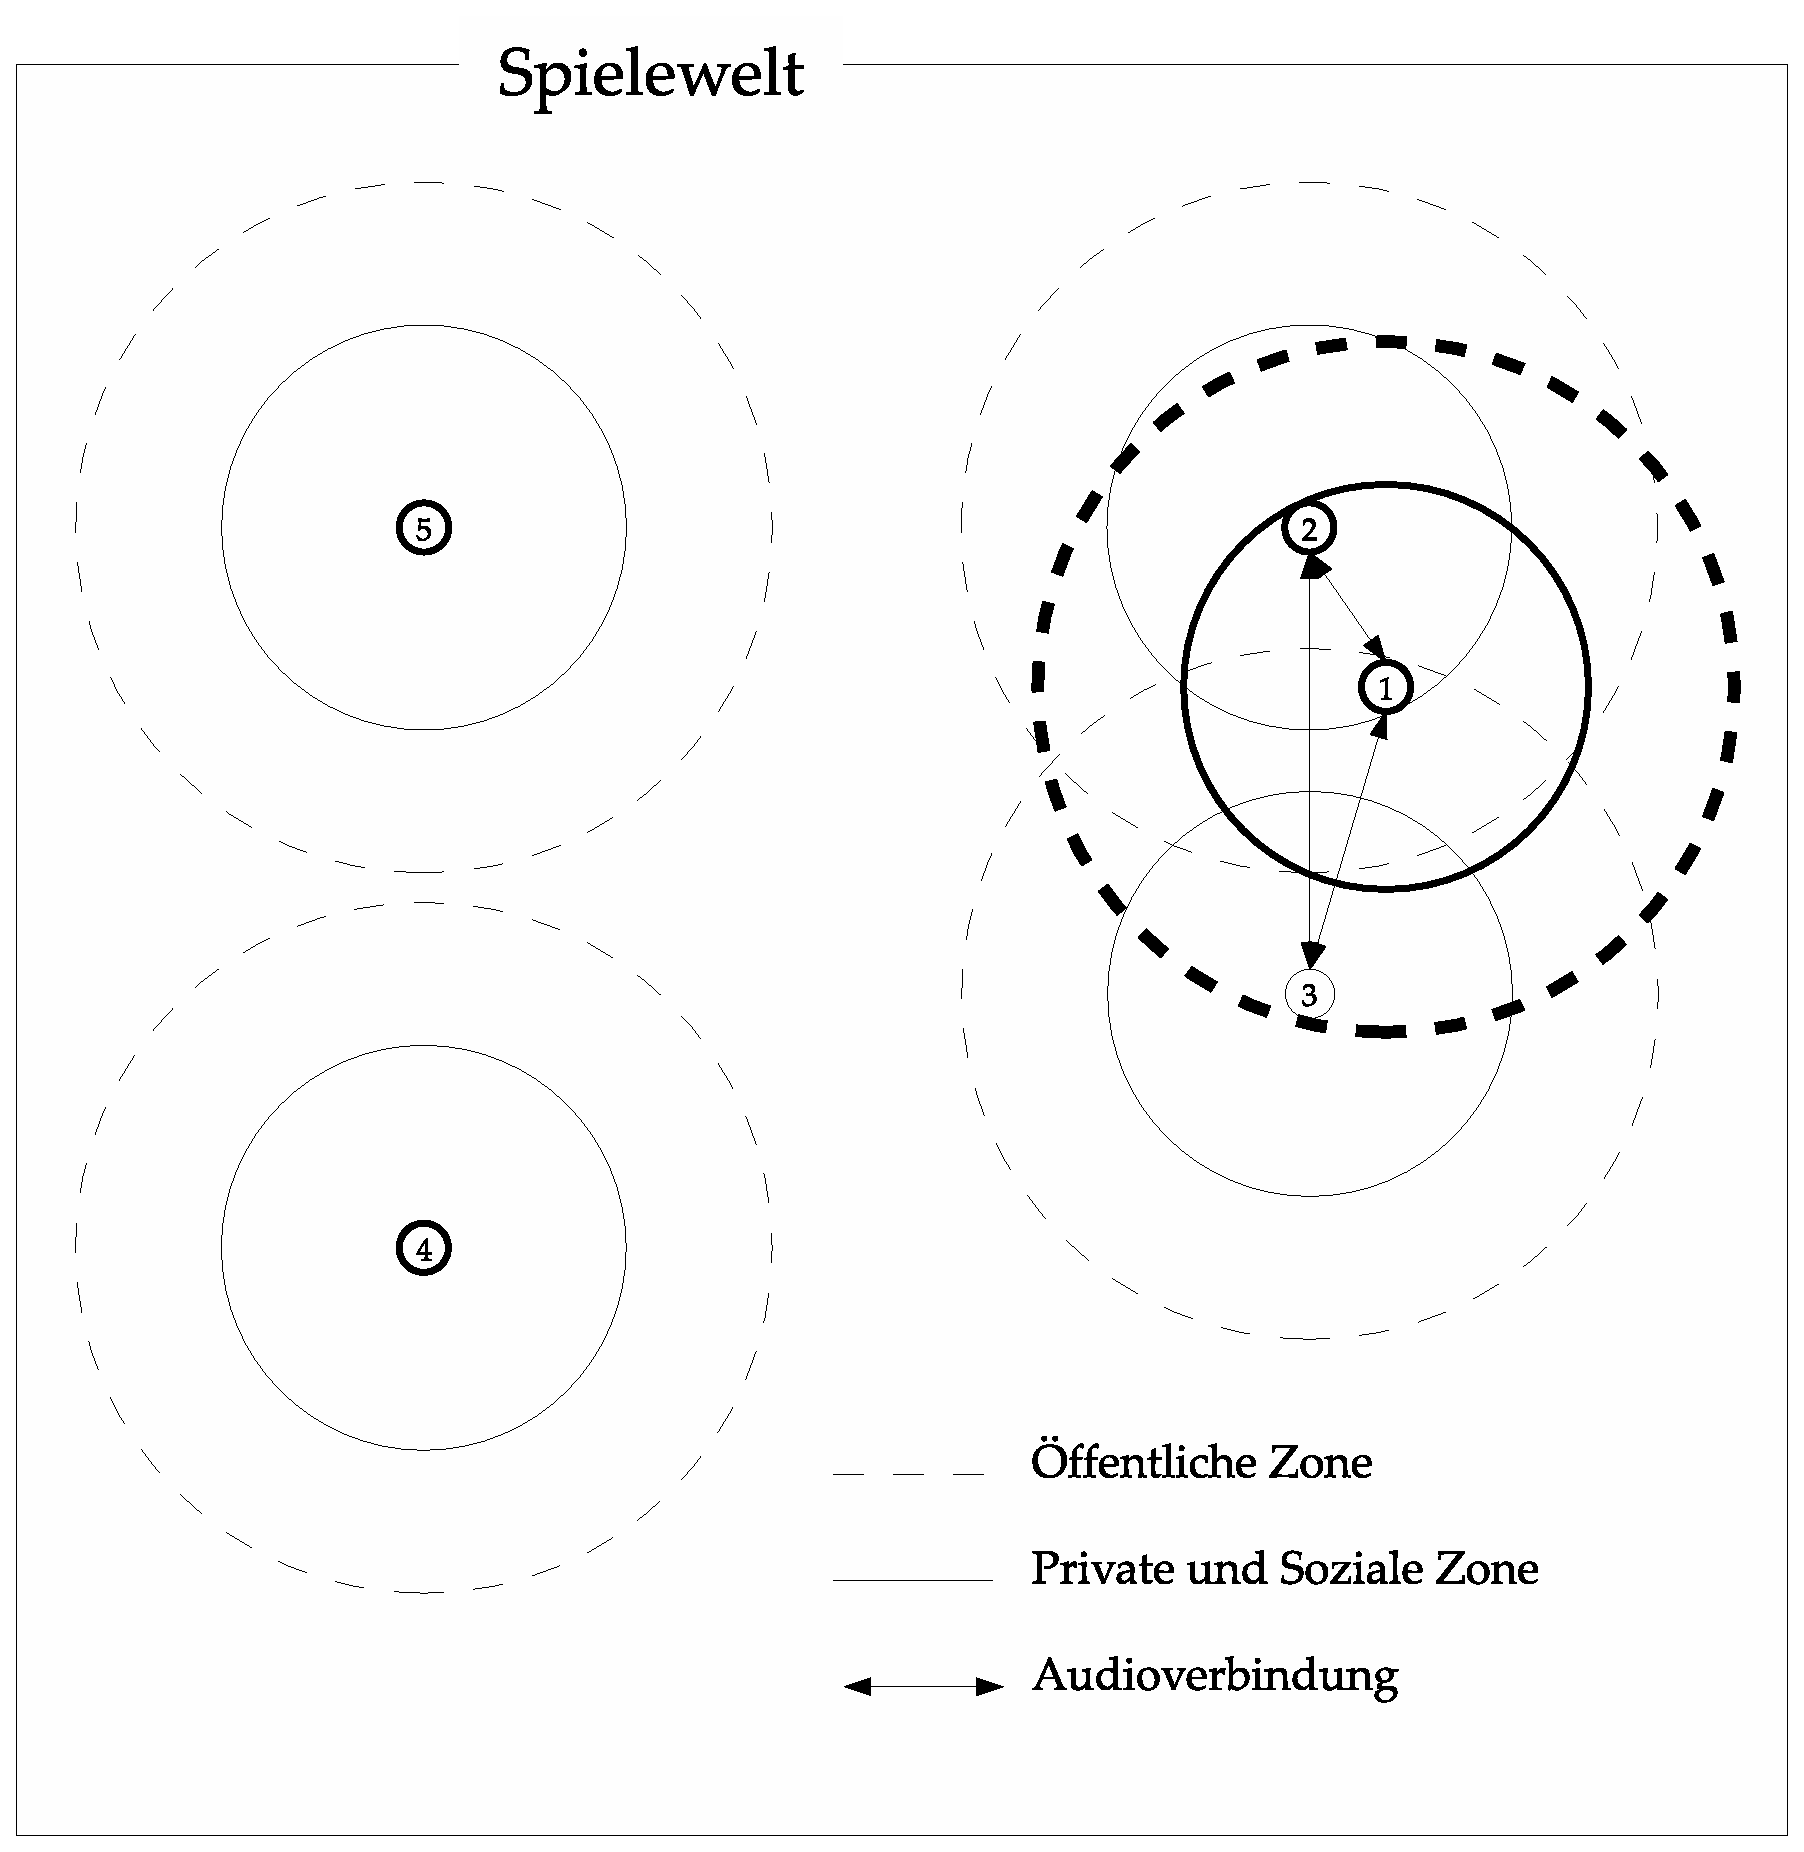
\includegraphics[width=.70\textwidth]{grafiken/partialmesh.eps}
%	\caption{Ein Partial-Mesh der Audioverbindungen der Teilnehmer}
%	\label{fig:partialmesh}
%\end{figure}

Abbildung \ref{fig:partialmeshchart} zeigt den Bandbreitenverbrauch von Teilnehmer 1 in Abh�ngig\-keit zur Anzahl der sich im Spiel befindlichen Spieler. Zum Zeitpunkt $t1$, in dem Spieler 2 das Spiel betritt, ist der Aufbau einer Audioverbindung erkennbar, die zwischen 10-15 KByte/s verbraucht. Zum Zeitpunkt $t2$ betritt Spieler 3 das Spiel, diesmal werden nur zus�tzliche 1-2 KByte/s zur Aufrechterhaltung der Grundkonnektivit�t ben�tigt, weil auf RTP-Ebene eine Silence-Suppression stattfindet. Spieler 4 und 5 dagegen verursachen keinen zus�tzlichen Bandbreitenverbrauch, denn sie befinden sich au�erhalb der �ffentlichen Zone und es werden keine Verbindungen zu ihnen aufgebaut. Im Vergleich zu Abbildung \ref{fig:fullmesh-withchart} werden hier insgesamt nur 16 KByte/s verbraucht, also eine Einsparung von 60\% vorgenommen. Man darf aber nicht vergessen, dass sich im Worst-Case alle Teilnehmer im gegenseitigen H�rradius befinden k�nnen, was dazu f�hrt, dass eine Full-Mesh-Topologie zwischen ihnen aufgebaut wird. Hier kann keine Bandbreite eingespart werden und das vorgestellte Verfahren verliert seinen Vorteil.

\begin{figure}[tbh]
	\centering
		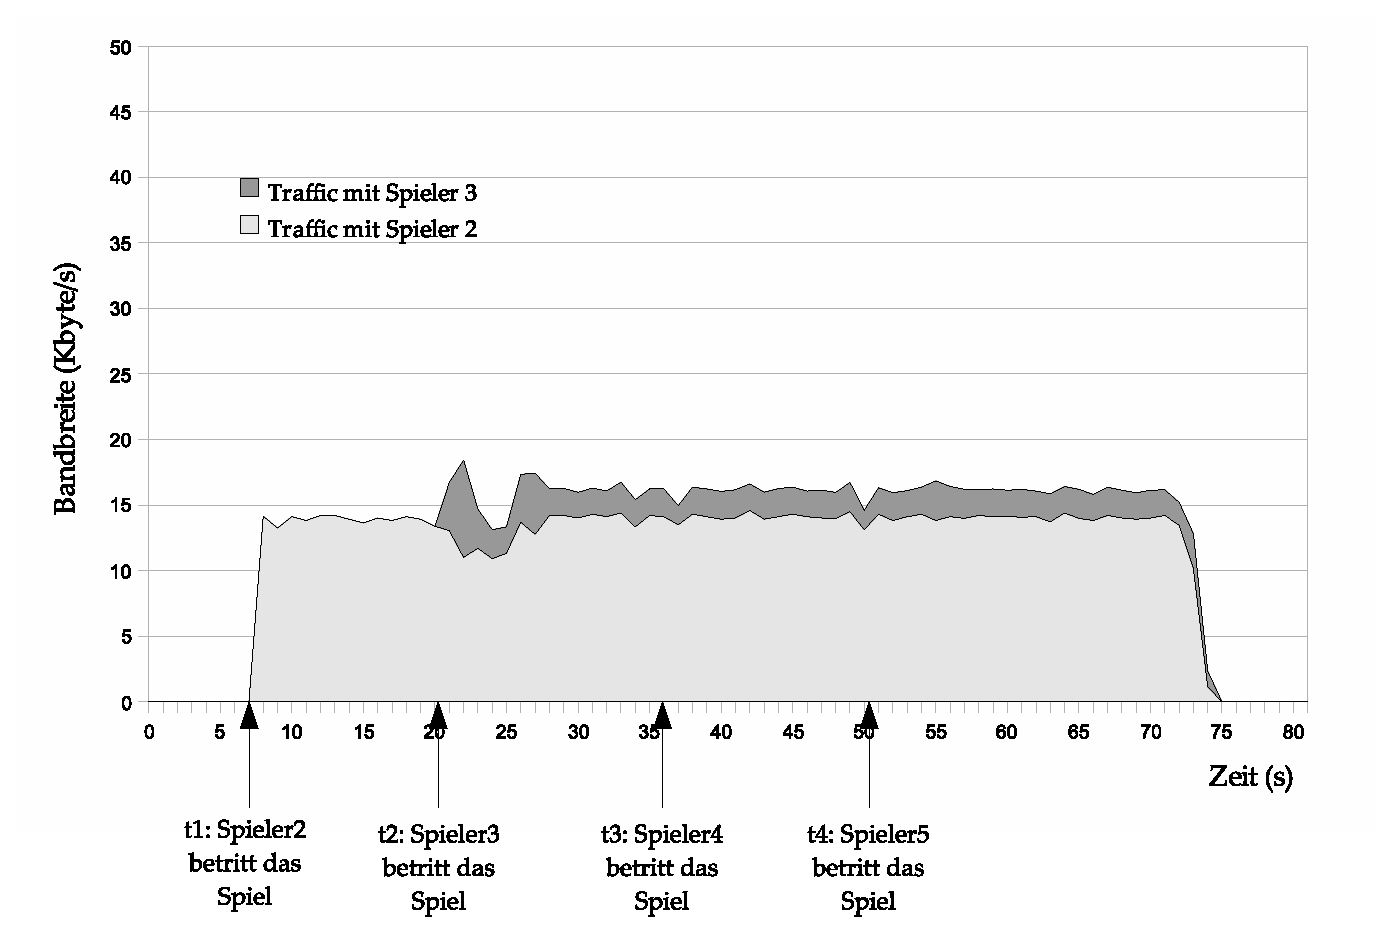
\includegraphics[width=\textwidth]{grafiken/partialmeshchart.eps}
	\caption{Resultierende Bandbreiteneinsparungen durch den Partial-Mesh-Ansatz, da nicht mehr alle Verbindungen aufgebaut werden m�ssen}
	\label{fig:partialmeshchart}
\end{figure}

%\begin{figure}[tbh]
	%\centering
		%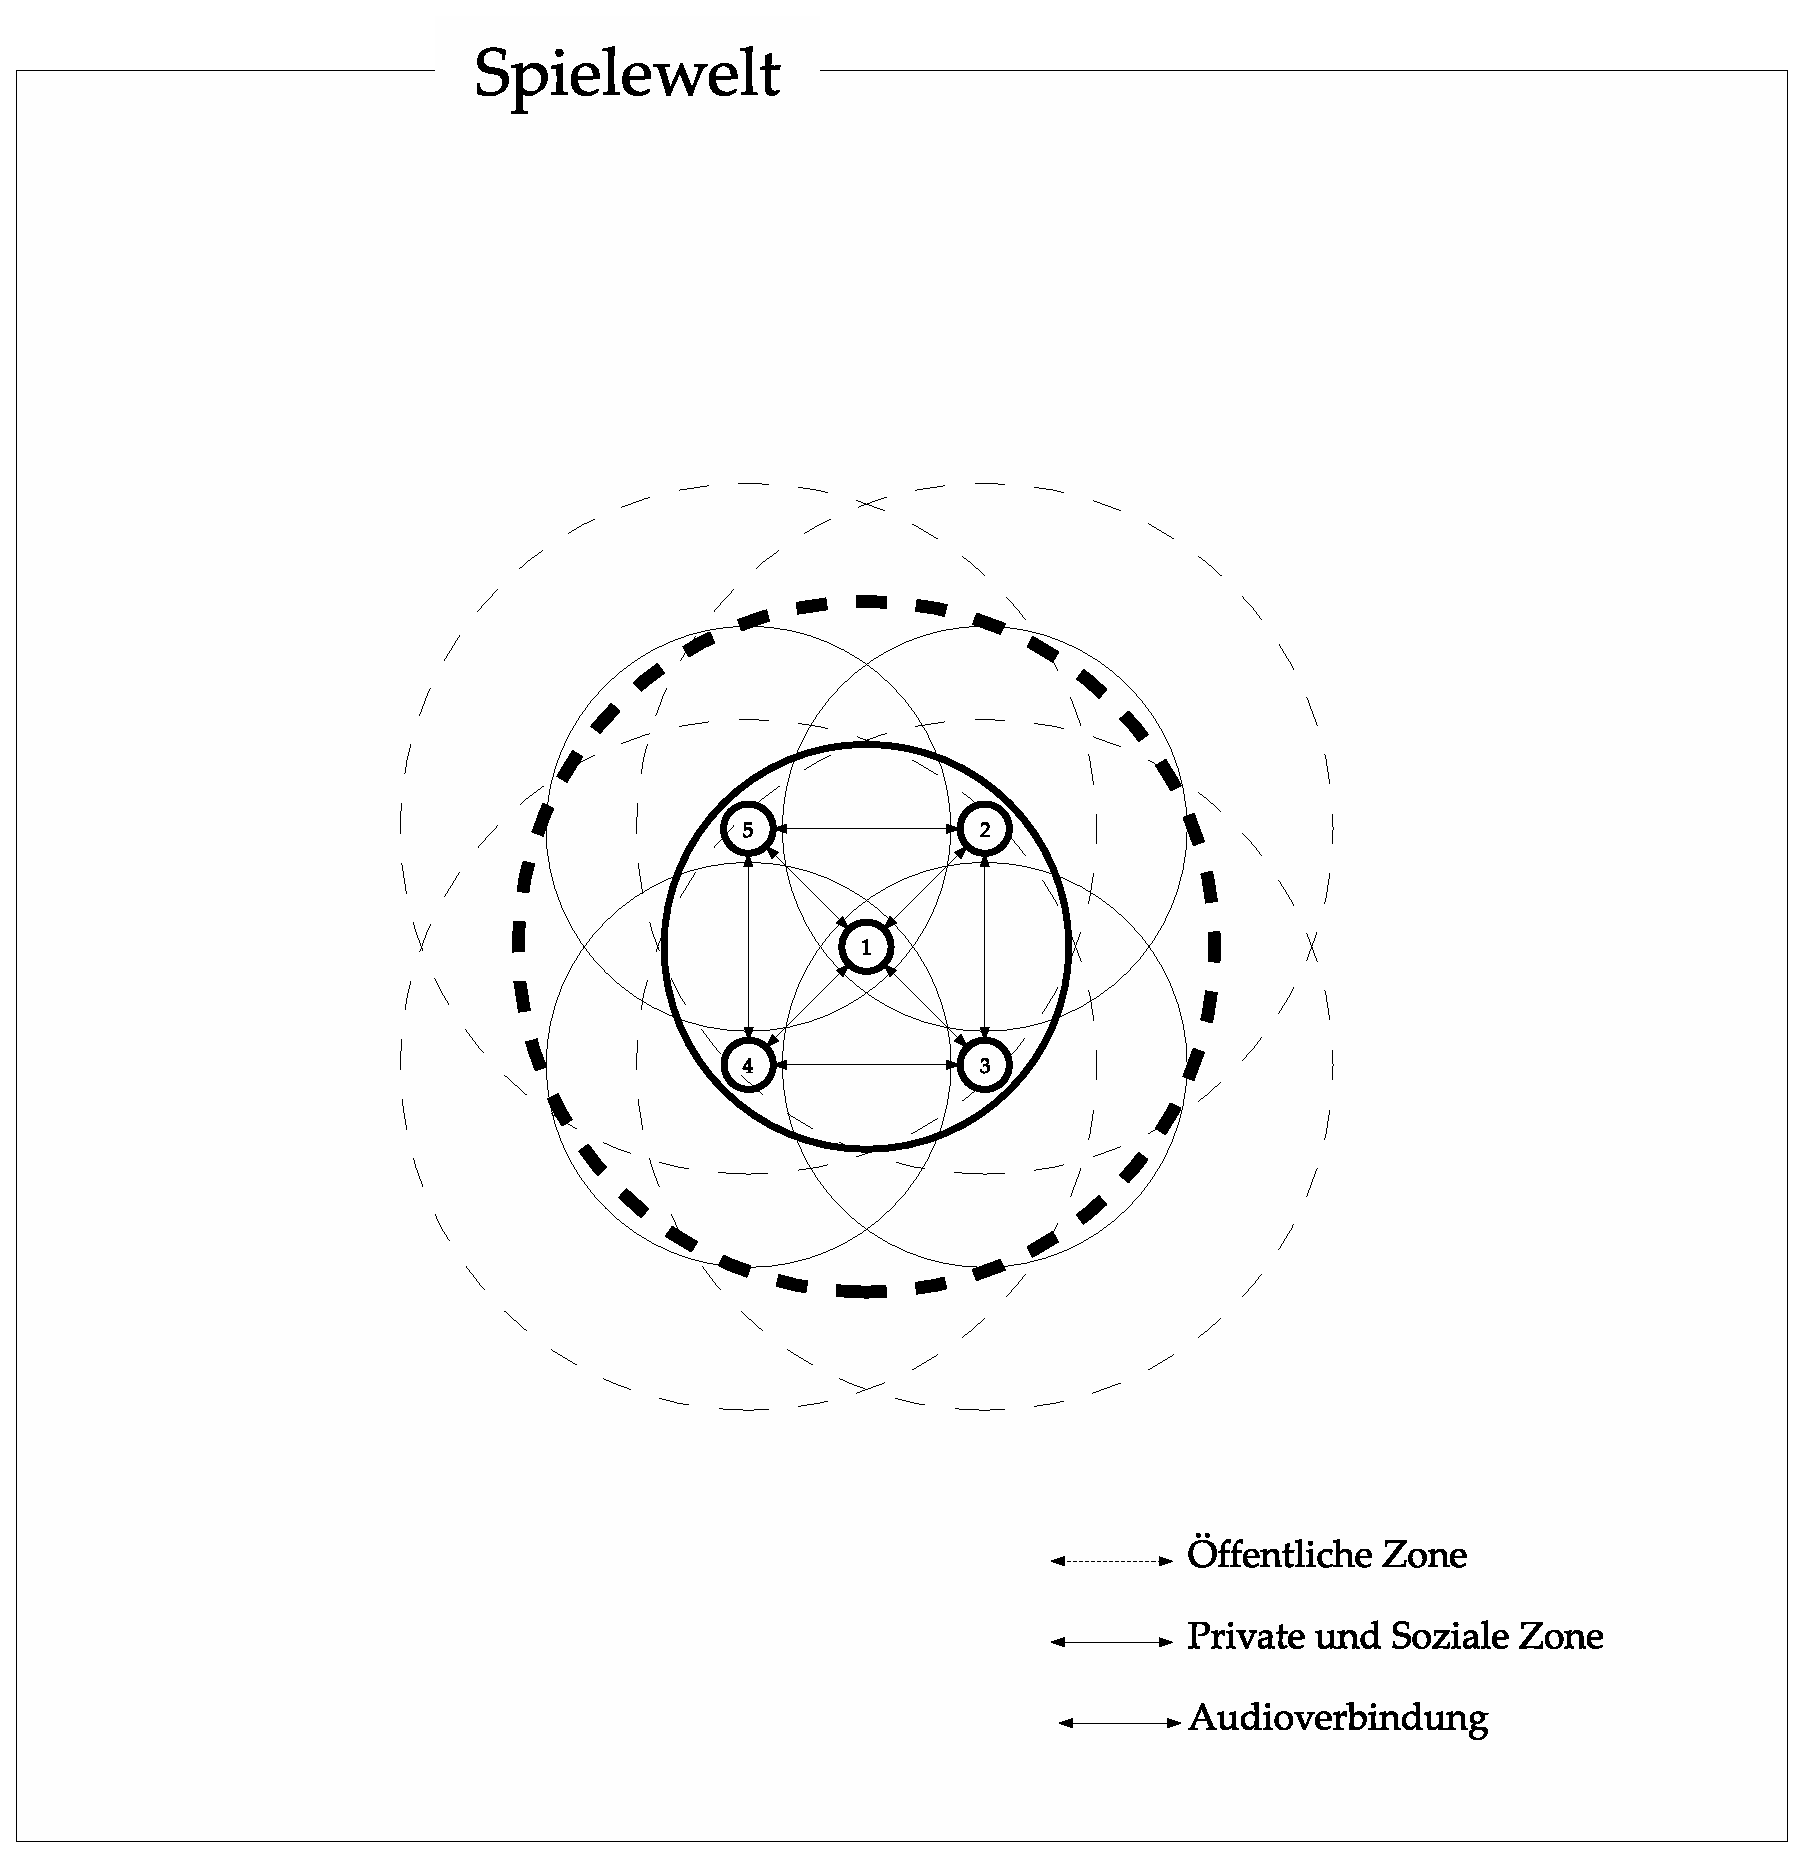
\includegraphics[width=0.70\textwidth]{grafiken/fullmesh-worstcase.eps}
	%\caption{Partial-Mesh "`Worstcase"'-Szenario gleicht einem Full-Mesh}
	%\label{fig:fullmesh-worstcase}
%\end{figure}

\section{Zonenkonzepte}
Um den Bandbreitenverbrauch in den einzelnen Zonen aufzuzeigen, wurde ein einfaches Szenario erstellt, bei 2 dem Spieler am gleichen Ausgangspunkt das Spiel beginnen und sich dann voneinander wegbewegen. W�hrend sie die einzelnen Zonen durchlaufen werden wird der Bandbreitenverbrauch eines Teilnehmers gemessen. Bei der Messung wird nicht nur zwischen dem Up- und Downloadverbrauch, sondern auch zwischen dem des SIP- und RTP-Protokolls unterschieden. F�r jede der  drei Implementierungsvariationen (RTP-Silence-Suppression, SIP-Hold, unterschiedliche Audiocodecs) wurde jeweils eine Messung vorgenommen. 

\subsection{Ohne Einsatz von Zonen}
Hier entfernen sich beide Spieler voneinander, es werden jedoch keine bandbreitenreduzierenden Ma�nahmen in Abh�ngigkeit von der Zone des Spielers getroffen. Man erkennt in der Abbildung \ref{fig:NOVADrtpsip} (siehe Anhang), dass die Bandbreite  in allen Zonen um 10 KByte/s liegt. 

Beim Vergleich der Bandbreite des RTP- und SIP-Protokolls in Abbildung \ref{fig:NoVADupdown}  zeigt der Plot, SIP wird nur zum Signalisieren des Anrufs benutzt, da es nur am Anfang und Ende des SIP-Anrufs Bandbreite erzeugt, w�hrend das RTP-Protokoll f�r den reinen Audiostrom zust�ndig ist.  

\subsection{Zonen mit RTP-Silence-Suppression}

Hier wird in der �ffentlichen Zone eine Silence-Suppression durchgef�hrt. In der Abbildung \ref{fig:VADupdown}  ist eine Reduktion des Bandbreitenverbrauchs auf unter 1kByte/s zu erkennen, w�hrend er in der privaten und sozialen Zone bei fast 10 KByte/s liegt.  

In der Abbildung \ref{fig:VADrtpsip} wurde ein Vergleich der SIP- und RTP-Protokolle dargestellt. Der Plot zeigt wieder, beim Einsatz der Silence-Suppression beim RTP Protokoll in der �ffentlichen Zone sinkt die Bandbreite auf unter 1 KByte/s. Anhand der Unterscheidung der beiden Protokolle wird deutlich, dass es sich um eine Eigenschaft des RTP-Protokolls handelt, da kein SIP-Nachrichtenverkehr beim �bergang zur �ffentlichen Zone flie�t. 

\subsection{Zonen mit SIP-Hold}

Eine weitere Unterscheidung der Zonen wurde mit dem SIP "`Hold Call-Ansatz"' versucht, bei dem in der �ffentlichen Zone mittels des SIP-Protokolls der logische Anruf gehalten wird, aber auf RTP-Ebene keine �bertragung der Pakete stattfindet. Wie Abbildung \ref{fig:mitholdupanddown} zeigt, kann dieser Ansatz sogar noch mehr Bandbreite in der �ffentlichen Zone als die Silence-Suppression einsparen, da praktisch kein Datenaustausch mehr stattfindet.

Allerdings konnte sich der SIP-Hold-Ansatz in der Praxis nicht bew�hren, denn beim Halten und Wiederaufnehmen des Gespr�chs werden, die Sitzungsparameter wieder neu verhandelt, was zu einer sp�rbaren Verz�gerung f�hrt. Es ist aber vorstellbar den SIP-Anruf schon etwas fr�her wiederaufzunehmen, um diese Verz�gerung auszugleichen und so beim Erreichen der sozialen Zone einen bereits etablierten Anruf vorzufinden. 

Beim Bandbreitenvergleich der SIP- und RTP-Protokolle sieht man, dass im Gegensatz zur Silence-Suppression, eine Signalisierung mit SIP beim �bergang von der sozialen zur �ffentlichen Zone stattfindet. 

\subsection{Zonen mit unterschiedlichen Audiocodecs}
\label{audiocodec-zonen}
Die dritte Variante beinhaltete den Einsatz von 2 verschiedenen Codecs f�r die private und soziale Zone. In der privaten Zone wurde der qualitativ hohe Speex-Codec mit einer Abtastrate von 16kHz verwendet, w�hrend in der sozialen Zone nur der Speex Codec mit einer Abtastrate von 8kHz zum Einsatz kam. 

Da erwartet wird, dass in der sozialen Zone mehr Verbindungen als in der privaten Zone aufgebaut werden, wird hier auch ein Codec mit einer niedrigeren Bitrate (11 KBit/s) verwendet, um eine gr��ere Anzahl an Verbindungen zu erm�glichen. In der �ffentlichen Zone wird wie im oberen Beispiel (siehe Abbildung \ref{fig:VADupdown}) die Silence-Suppression angewendet. In \ref{fig:mitvadund2codecs} ist zu sehen, dass der der Bandbreitenverbrauch in der sozialen Zone mit 7 KByte/s im Vergleich zur privaten Zone mit 9 KByte/s um 23\% reduziert wird. In der �ffentlichen Zone wird fast 90\% der Bandbreite eingespart. 

Im Vergleich (siehe Abbildung \ref{fig:mitvadundrtpsip}) der beiden SIP- und RTP-Protokolle ist beim SIP-Protokoll sowohl der Rufauf und -abbau zu sehen als auch die Signalisierung des anderen Audiocodecs beim �bergang von der privaten in die soziale Zone. Beim RTP-Protokoll ist die �bertragung des Audiostroms und die reduzierte Bitrate in der sozialen und �ffentlichen Zone zu erkennen. 

An den vorgestellten Beispielen und Messungen sieht man, dass in einer distanzbasierten Sprachkommunikation erfolgreich verschiedene Verfahren eingesetzt wurden, um eine Unterscheidung der Bandbreite in Abh�ngigkeit von der Entfernung der Teilnehmer vorzunehmen. 
%//TODO Speex VBR and ABR is it possible?

%\subsection{SIP Benchmarks}
%\subsection{Mixing}
%-- Verbrauch der CPU Last mit Zunehmender Nutzerzahl beim Full Mesh 
%-- Verbrauch der CPU Last mit Zunehmender Nutzerzahl beim Partial Mesh
%--> M�sste zeigen dass weniger Streams gemischt werden m�ssen und somit Last eingespart werden %kann. ( Wie messe ich das?)
%MESSUNG: einfach nur die conference bridge messen.

\section{SIP als Netzwerkschnittstelle}

\begin{figure}
	\centering
		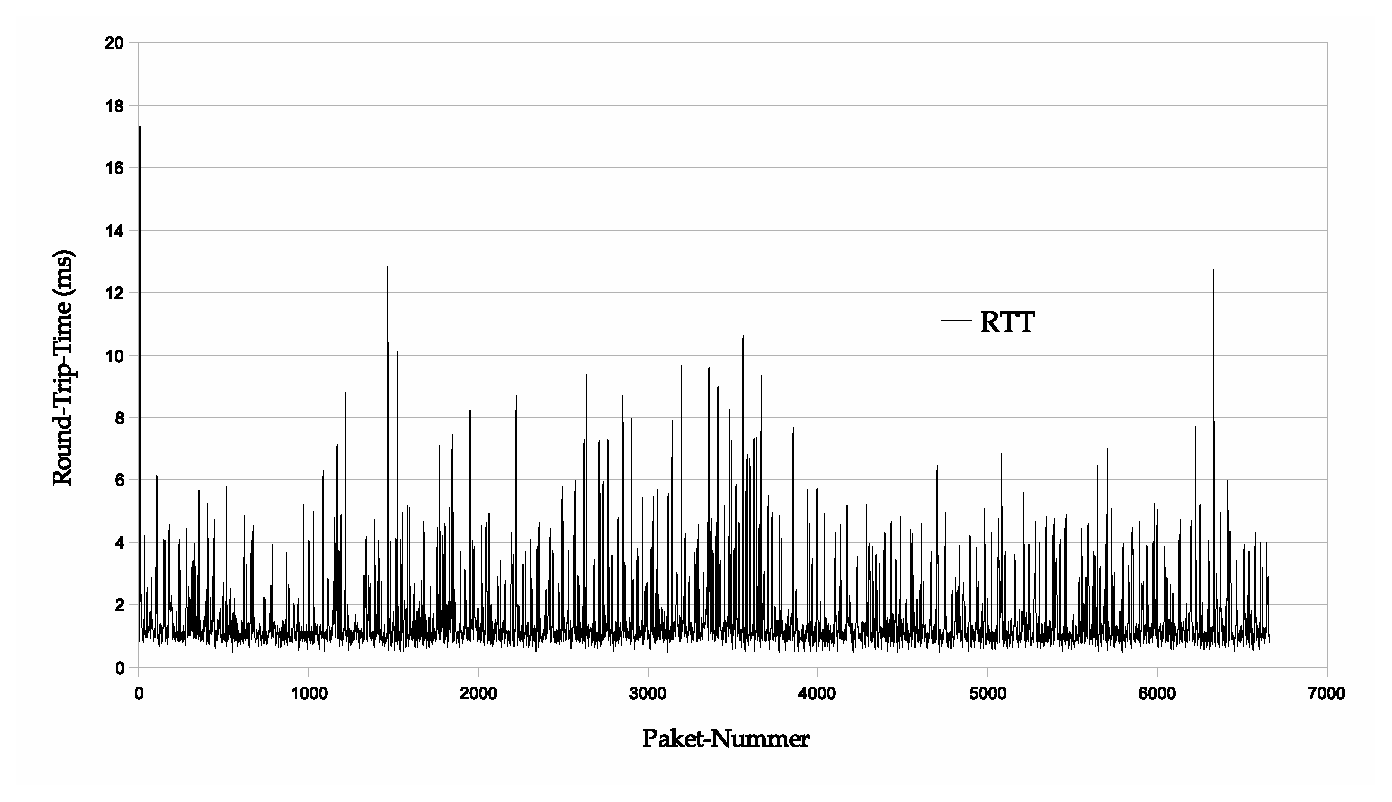
\includegraphics[width=1.00\textwidth]{grafiken/rtt-chart.eps}
	\caption{Messung der RTT im LAN zwischen zwei Clients}
	\label{fig:rtt-chart}
\end{figure}

F�r einen Test von SIP als Netzwerkschnittstelle wurden die 2 Desktop-Rechner aus dem Testaufbau (siehe Abschnitt \ref{testumgebung}) eingesetzt, die sich im Spiel befinden und gegenseitig ihre Rotations- und Positionsinformationen austauschen. Spielerechner und Proxy befanden sich in einem LAN. Die Messung selbst wurde auf dem Proxy vorgenommen, indem alle versendeten Pakete protokolliert und ausgewertet wurden. 

Um festzustellen, inwiefern die SIP-Abstraktionsebene die Netzwerk-Kommuni\-kation verz�gert, wurde die Round-Trip-Time (RTT) gemessen, die angibt wie lange ein Datenpaket in einem Rechnernetz ben�tigt, um von der Quelle zum Ziel und zur�ck zu reisen. Dabei wird hier die RTT zwischen dem Versand der MESSAGE-Nachricht und dem Empfang der 200-OK-Nachricht gemessen. dh. sie beinhaltet auch die Verarbeitung und Erstellung der Nachricht beim Quell-/Zielrechner.

Der Plot der RTT-Messung in Abbildung \ref{fig:rtt-chart} zeigt die gemessene RTT beim Versand von �ber 6000 Nachrichten. Diese liegt im Durchschnitt bei 1-2 ms und weist auch Verz�gerungen bis zu 13ms auf. Da die RTT in einem LAN �blicherweise 1ms betr�gt\footnote{Christoph L�ders, Martin Winkler: Pingpong. in: c't. Hannover 2006,23, S.199. ISSN 07248679} liegt die Verz�gerung durch den Einsatz von des SIP-Abstraktionslayers bei ca. 1 - 12 ms, was einen akzeptablen Wert darstellt.

\section{Conference-Bridge}
Um zu Messen, wie sich die Conference Bridge beim Mischen verschiedener Audiostr�me verh�lt, wurde die CPU-Auslastung eines Mixers auf einem Athlon-Duo 4600+ Rechner mit 3GB RAM, gemessen. Dazu wurde die Conference Bridge verwendet, um k�nstlich erzeugte Sinus-Audiosignale zu mischen. Obwohl kein Encoding und Decoding verwendet wird, zeigt die Grafik \ref{fig:confbench}, dass bereits beim Einsatz von Resampling bei 32 Teilnehmern die Kapazit�tsgrenze des Rechners erreicht wurde. Diese Messung st�tzt die Annahme aus Kapitel \ref{zentralansatz}, dass Mixing-Server zwar die entsprechende Bandbreite besitzen, um tausende von  Audiostr�men entgegenzunehmen, jedoch praktisch aufgrund ihrer CPU-Kapazit�t nicht in der Lage sind, in einer Konferenz so viele Audiostr�me zu mischen. 

\begin{figure}
	\centering
		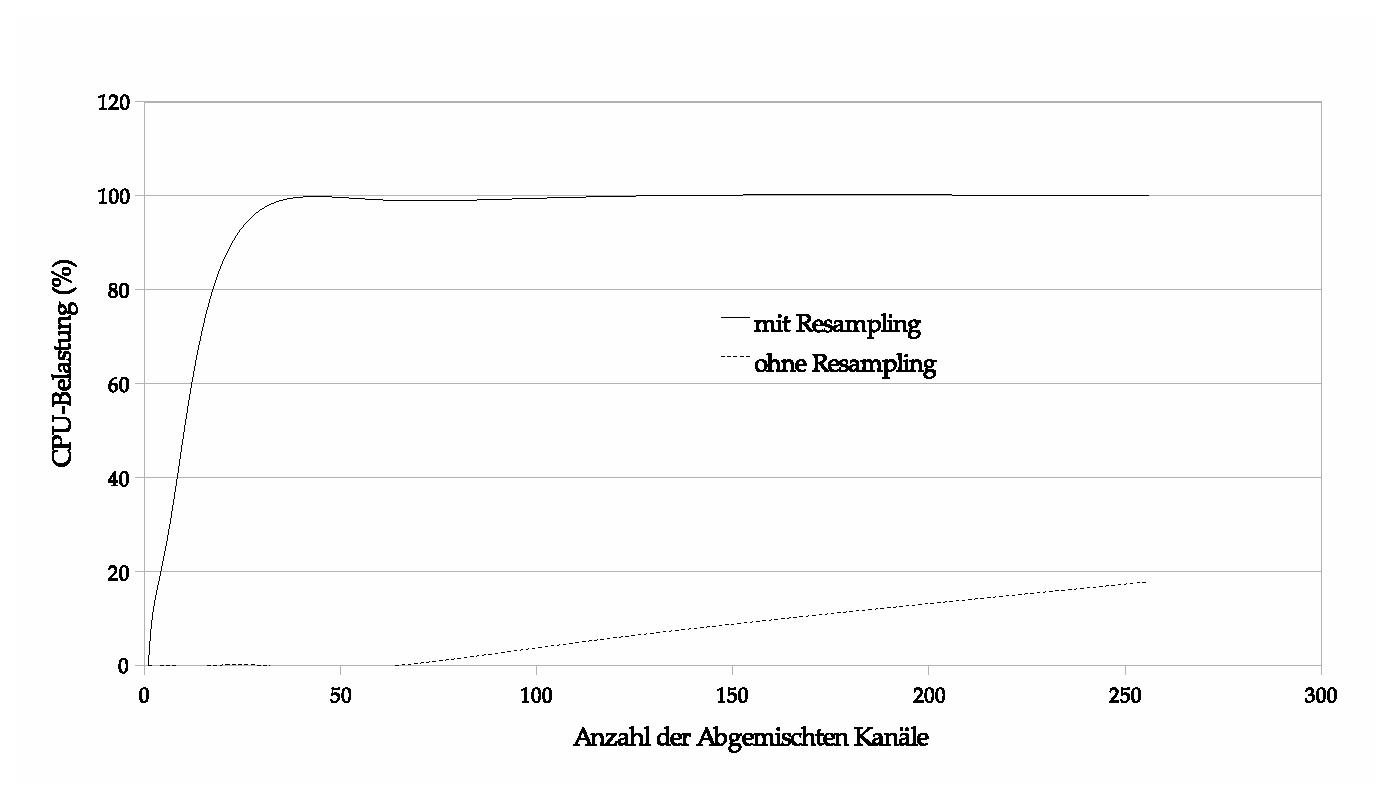
\includegraphics[width=1.00\textwidth]{grafiken/confbench.eps}
	\caption{Anstieg der CPU-Last in Abh�ngigkeit der Anzahl der abgemischten Audiokan�le}
	\label{fig:confbench}
\end{figure}
\cleardoublepage
\newpage~
\chapter{Fazit und Ausblick}

Das Ziel dieser Arbeit ist es eine Peer-to-Peer Sprachkommunikation zu implementieren, die einerseits durch ihre Architektur aber auch durch einen distanzbasierten Ansatz dazu beitragen soll relevante Probleme im Bereich der Audiokommunikation in Mehrspielerspieler Computerspielen zu l�sen. Dieses Kapitel beinhaltet ein kurzes Fazit der Ausarbeitung und stellt noch einmal die wichtigsten Punkte heraus.

\section{Fazit}
Der Grundlagenteil dieser Abhandlung zeigt zun�chst die bisherigen Schw�chen textbasierter Kommunikation in Computerspielen auf und nennt wichtige Gr�nde f�r die rasche Entwicklung der Sprachkommunikation im Spielesektor. Jedoch kann auch die Audiokommunikation nicht alle Probleme der Textkommunikation l�sen und bringt sogar auch eigene neue mit. Anhand der Metaanalyse ausgew�hlter Studien werden die wesentlichsten dieser vorgestellt und k�nnen auf drei Hauptursachen zur�ckgef�hrt werden: Den Einsatz von Drittanbieter L�sungen, die nicht in das Spiel integriert werden, die fehlende Flexibilit�t und Skalierbarkeit von bisher eingesetzter Client-Server Architekturen und die fehlenden Metaphern f�r eine �bertragung von Sprache in Computerspielen.

 Die Analyse bisheriger L�sungen zeigt, dass Teilnehmer der f�r diese typischen Massenkonferenzen nicht in der Lage sind zu bestimmen welchen Spieler sie adressieren wollen und auch keine Kontrolle dar�ber haben, wessen Audiosignal sie empfangen m�chten. Durch fehlende Metaphern, finden Spieler es schwer das Gesprochene in den Kopfh�rern mit den Avataren auf ihren Monitoren zu verkn�pfen. Spieler sind auf den Einsatz kostenpflichtiger Konferenzserver angewiesen, da das Abmischen des Audiostroms bisher zentral vorgenommen wird, was mit einer hohen Kapazit�tsauslastung solcher dedizierten Server verbunden ist.

In dieser Arbeit werden genau diese Unzul�ngl�nglichkeiten adressiert und L�sungen vorgeschlagen. Um die Brauchbarkeit dieser Vorschl�ge zu �berpr�fen wird im praktischem Teil der Arbeit ein Prototyp eines Computerspiels entwickelt, der �ber eine integrierte Sprachkommunikationsl�sung verf�gt. Es werden verschiedene Architekturen auf Basis des SIP Protokolls vorgestellt und kritisch analysiert. Es wird vor allem eine Unterscheidung zwischen dem Audiostrom und der Signalisierung und Lokation vorgenommen. Vor allem im Bereich von Peer-to-Peer Architekturen werden neue Konzepte vorgeschlagen um Bandbreite einzusparen. Es wird gezeigt wie durch den Partial-Mesh Ansatz, bei dem nur Verbindungen mit Teilnehmern in der N�he des Spielers aufbaut werden Bandbreite eingespart werden kann. Ein weiterer Ansatz nutzt verschiedene Audiocodecs in Abh�ngigkeit der Entfernung der Spieler zueinander.

Durch den Einsatz von Peer-to-Peer Audio�bertragungen und der daraus resultierenden client-seitigen Kontrolle des Audiostroms ist es m�glich gewesen die gesetzten Ziele zu erf�llen: So konnte die Metapher der �bertragung der Sprache durch die Luft realisiert werden und dieses Konzept dazu genutzt werden neue und intuitive Wege der Konferenzsteuerung aufzuzeigen. Durch den Empfang aller ben�tigter Audiostr�me sind Spieler zum ersten Mal in der Lage ihre pers�nliche Konferenz zu erzeugen, die in Abh�ngigkeit der Distanz der Spieler voneinander eine pers�nliche oder �ffentliche sein kann. 

Theoretische Konzepte aus der werden Proxemik direkt in die Praxis umgesetzt, indem ein 3 Zonen Modell erstellt wird, dass verschiedene Konnektivit�tsstufen zwischen den Spielern erlaubt. Der Raum des Spielers wird in eine private, soziale und �ffentliche Zone unterteilt, die jeweils verschiedene Funktionen besitzen. Die private Zone dient der interpersonellen Kommunikation, die soziale der Massenkommunikation und die �ffentliche der Aufrechterhaltung einer Grundkonnektivit�t bei mehreren Spielern. 

Dieses Modell bildet auch die Ausgangsgrundlage, um das schwierige Problem des quadratisch ansteigenden Bandbreitenverbrauchs beim Peer-to-Peer Ansatz zu adressieren. Dazu werden Mechanismen des SIP und RTP Protokolls ausgenutzt, um f�r verschiedene Zonen unterschiedliche Bandbreitenanforderungen zu erf�llen. Es wird die SIP Hold Technik genutzt, die RTP Silence Suppression und verschiedene Audiocodecs f�r verschiedene Zonen. Anhand Messungen wird in der Evaluation der Implementierung verdeutlicht, dass ein Gro�teil von Verbindungen und entsprechender Bandbreite eingespart werden kann, wenn nur Verbindungen mit Spielern, die sich auch in Reichweite des Spielers befinden, etabliert werden und die Audiokommunikation mit weiter entfernten Spielern einer gr��eren Kompression unterliegt.

Da das verwendete SIP Protokoll nicht nur als reines Signalisierungsprotokoll f�r Sprach�bertragungen verwendet werden kann, sondern auch als Netzwerkschicht zum Austausch von Spielezust�nden und Informationen genutzt werden kann, werden in der Implementierung bestehende Komponenten und Dienste so eingesetzt, dass der Spielprototyp auf Grundlage des SIP und SIMPLE Protokolls implementiert werden konnte. In einem Abschlie�enden Diskurs wird die Tauglichkeit von SIP als Grundlage f�r P2P Spiele diskutiert und ein theoretischer Ansatz veranschaulicht.

\section{Ausblick}
Im Laufe der Diplomarbeit ergaben sich einige interessante Fragestellungen, deren Beantwortung lohnende Erkenntnisse in Bezug auf die Zukunft von Sprachkommunikationsl�sungen in Mehrspieler Computerspielen liefern k�nnen. 

Das in dieser Arbeit vorgestellte Konzept greift viele bisherige Unzul�nglichkeiten der Sprachkommunikation auf, zeigt auch Verbesserungsvorschl�ge, die sich allerdings erst in einem Test mit einer gr��eren Anzahl an professionellen Teilnehmern behaupten m�ssen. Daraus k�nnten interessante Erkenntnisse gewonnen werden, ob das Zonenkonzept tats�chlich genutzt wird und ob die Metapher der �bertragung des Schalls durch die Luft positiv aufgenommen wird. Genauso k�nnten auch Schwachpunkte eines solchen Ansatzes evaluiert werden. 

Trotz des Bem�hens die Bandbreitenanforderungen in der Sprachkommunikation minimal zu halten, wurden die architekturbedingten Grenzen eines reinen P2P Ansatzes deutlich. Ein multi unicast Ansatz ger�t bei einer hohen Avatardichte schnell an seine Grenzen, da der Bandbreitenverbrauch mit jedem weiterem Benutzer quadratisch ansteigt. Um eine hohe Avatardichte mit mehreren hundert Mitspielern zu erm�glichen, sind L�sungen gefragt, bei denen einzelne \textit{Superpeers} in der Lage sind Audiostr�me intelligent abzumischen. Solche intelligenten L�sungen sollten Teilnehmern die gleiche Flexibilit�t und Kontrolle �ber den Audiostrom zu liefern wie ein multi unicast Peer-to-Peer Ansatz, aber gleichzeitig den Bandbreitenverbrauch eines einzelnen Peers reduzieren k�nnen. 

Eine weitere zuk�nftige Herausforderung liegt darin, einen v�llig dezentralen P2P Overlay aufzubauen, der �ber keine zentrale Komponenten verf�gt. In diesem Overlay sollten sowohl der Austausch an Audiostr�men als auch jegliche Signalisieruns-, Rechte- und Lokations-Anfragen v�llig dezentral stattfinden. Momentan ben�tigt die in der Arbeit vorgestellte Implementierung einen zentralen Lokationsdienst. 
Der zuk�nftige Einsatz von P2P SIP, welches in dieser Arbeit n�her erl�utert wird, bietet ein L�sung, die bei gleicher Abstraktionsebene ohne zentrale Komponenten auskommt. Es ist sehr wahrscheinlich, dass in kurzer Zeit SIP Frameworks existieren, in denen die Komponente des Registrars verteilt realisiert wird. Diese bilden die optimale Grundlage f�r eine v�llig dezentrale Kommunikation oder ganze P2P Spiele.

Obwohl zwar mehrere Sprachkommunikations L�sungen auf Basis von propri�teren L�sungen existieren, ist es durchaus vorstellbar, dass die Standardisierung im kommerziellen VoIP Bereich, auch im Spielebereich Einsatz h�lt. Ein offenes Protokoll wie z.B. SIP k�nnte  helfen Anbieterl�sungen kompatibel zu machen. 

Bisher muss festgehalten werden, dass eine integrierte Sprachkommunikation von den wenigsten Spielerherstellern unterst�tzt wird. Noch scheuen sie den technischen Aufwand und die mit der Entwicklung und Betrieb verbundenen Kosten von integrierten Konferenzl�sungen. Diese Arbeit hat jedoch gezeigt, dass mit der immer gr��er werdenden Popularit�t des SIP Protokolls und dem Trend zu Peer-to-Peer Anwendungen, in naher Zukunft auch kleinere Studios praktikable integrierte Sprachkommunikationsl�sungen anbieten k�nnen. Da bei einer P2P Architektur keine eigene Infrastruktur n�tig ist und Bandbreite und Leistung vom Anwender selbst gestellt werden, sind die wichtigsten Kostenfaktoren nicht mehr vom Betreiber zu tragen. 

Der Einsatz von Sprachkommunikation in Handyspielen oder tragbaren Konsolen\footnonte{Nintendo DS, Playstation Portable} k�nnte Spielern zum ersten Mal die M�glichkeit geben miteinander zu kommunizieren auch wenn ihre Endger�te �ber keine Tastatur verf�gen.

Mit der konsequenten Anwendung von Metaphern zur Sprach�bertragung k�nnen Spiele ganz neue taktische Aspekte bekommen. Das Belauschen von gegnerischen Teams, der Einsatz von Funksprechger�ten, Wanzen, Satelitentelefonen, neue Spielerrollen wie Funker, Kommandeur, oder Spion sto�en f�r Spieler eine ganze Welt von M�glichkeiten auf.

Durch eine Integration der bestehender VoIP Standards in Computerspiele w�rden f�r Spieler die Grenzen zwischen dem Spiel als Unterhaltungsplattform und dem Spiel als Kommunikationsplattform verschwimmen. Das Finden von Mitspielern f�r eine Sitzung wird somit bereits Teil des Spiels. Das von SonyEntertainment auf der 'Game Developers Conference' am 7ten M�rz 2008 f�r die Playstation 3 Konsole vorgestellte 'Home System'  \footnote{Sony Entertainment, Version 02.04.2008, http://playstationhome.com/}, vereint genau diese Funktionalit�ten. 

Der Trend zu Spielerinteraktion, als fundamentalem Bestandteil von Computerspielen \cite{gibbs05}, wird in Zukunft in den Wohnzimmern von einem breiten Publikum entschieden. Durch die Kombination einer einfachen, intuitiven Sprachkommunikation mit realisitschen virtuellen 3D Welten k�nnten sog. "`Third Places"' \cite{gibbs03} entstehen, in denen Spieler die sozialen Netzwerke von Morgen kn�pfen. 

//TODO
3D Positionierung

%\subsubsection{Mobile Einsatzbereiche}
%Ein untersch�tztes Nebenprodukt des Einsatzes der Sprachkommunikation ist, dass man aufgrund nicht ben�tigter Tastatur auch bei mobilen Ger�ten die M�glichkeit hat miteinander zu Kommunizieren. So ist es vorstellbar auf tragbaren Konsolen Mittels VoIP und Wlan Spiele miteinander zu spielen und gleichzeitig zu kommunizieren. 


%\subsubsection{Freundschaften kn�pfen}
%Mittels VoIP ist es bereits heute m�glich und �blich mit Freunden und bekannten auf der ganzen Welt kostenlos zu telefonieren. Obwohl soziale Netzwerke im Internet ein Spiegel der real existieren Netzwerke sind, bieten Spiele die M�glichkeit sich �ber die Methode des gemeinsamen Erlebens Freundschaften zu Entwickeln. Gerade im Spielebereich ist eine starke Bindung zu Spielergruppen �blich. Mit Sprachkommunikation k�nnen st�rkere Bindungen der Spieler untereinader erfolgen, und mittels einer interpersonellen Sprachkommunikation im Spiel auch pers�nliche Themen diskutiert werden, w�hrend man gemeinsam seine Freizeit im von Third Place verbringt \cite{gibbs03}.

%\subsubsection{Standardisierung}
%Obwohl mehrere Sprachkommunikations L�sungen auf Basis von propri�teren Technologie existieren, ist es durchaus vorstellbar, dass die Standardisierung die im VoIP bereits weit gediegen ist, auch im Spielebereich Einsatz h�lt. So ist es vorstellbar, dass Sprachkommunikation auf einem offenen Protokoll wie z.B. SIP basieren kann und Anbieterl�sungen somit kompatibel werden.




\newpage~
%

\chapter{Summary, Conclusions, and Further Work}
\label{chap:conclusions}
The purpose of this book is to understand  the influence of representations on the performance of genetic and evolutionary algorithms. 
This chapter summarizes the work contained in this study and lists its major contributions.

\selectlanguage{english}
\section{Summary}

We  started in Chap.~\ref{chap:einleitung} by providing the necessary background for examining representations for  GEAs. Researchers recognized early that representations have a large influence on the performance of GEAs. Consequently, after a brief introduction into representations and GEAs, we discussed how the influence of representations on problem difficulty  can be measured. The chapter ended with prior guidelines for choosing high-quality  representations. Most of them are  mainly based on empirical observations and intuition and not on theoretical analysis.

Therefore, we presented in Chap.~\ref{cha:grafiken} three aspects of a theory of representations for  GEAs. We investigated how the locality, scaling, and locality of an encoding  influences GEA performance. The performance of GEAs is determined by the solution quality at the end of a run and the number of generations until the population is converged. Consequently, for redundant and exponentially scaled encodings, we presented population sizing models and described how the time to convergence is changed.
Furthermore, we were able to demonstrate that high-locality encodings do not change the difficulty of a problem; in contrast, when using low-locality encodings, on average, the difficulty of problems changes. Therefore,  easy problems become more difficult and difficult problems become easier by the use of low-locality encodings.
For all three properties of encodings, the theoretical models were verified with empirical results.


\section{Conclusions}
We  summarize the most important contributions of this work.

{\bf Framework for design and analysis of representations (and operators) for GEAs.} The main purpose of this study was to present a  framework which describes how genetic representations influence the performance of GEAs. The performance of GEAs is measured by the solution quality at the end of the run and the number of generations until the population is converged. 
The proposed framework allows us to analyze the influence of existing representations on GEA performance and to develop efficient new representations in a theory-guided way.
Furthermore, we illustrated that the framework can also be used for the design and analysis of search operators, which are relevant for direct encodings.
Based on the framework, the development of high-quality representations remains not only a matter of intuition and random search but becomes an engineering design task.
Even though more work is needed, we believe that the results presented are sufficiently compelling to recommend increased use of the framework.



{\bf Redundancy, Scaling, and Locality}. These are the three elements of the proposed framework of representations.  We demonstrated that these three properties of representations influence GEA performance and presented theoretical models to predict how solution quality and time to convergence changes.
By examining the redundancy, scaling, and locality of an encoding, we are able to predict the influence of representations on GEA performance.

The theoretical analysis shows that the redundancy of an encoding influences the supply of building blocks (BB) in the initial population. $r$ denotes the number of genotypic BBs that represent the best phenotypic BB, and $k_r$ denotes the order of redundancy. For synonymously redundant encodings, where all genotypes that represent the same phenotype are similar to each other, the probability of GEA failure goes either with  $O(\exp(-r/2^{k_r}))$ (uniformly scaled representations) or  with $O(\exp(-\sqrt{r/2^{k_r}}))$ (exponentially scaled representations).
Therefore, GEA performance increases if the representation overrepresents high-quality BBs. If a representation is uniformly redundant, that means each phenotype is represented by the same number of genotypes, GEA performance remains unchanged in comparison to non-redundant encodings.

The analysis of the scaling of an encoding reveals that non-uniformly scaled representations modify the dynamics of genetic search. If exponentially scaled representations are used, the alleles are solved serially which increases the overall time until convergence and results in problems with genetic drift but allows rough approximations of the expected optimal solution after a few generations.

We know from previous work that the high locality of an encoding is a necessary condition for efficient mutation-based search.
An encoding has high locality if neighboring phenotypes correspond to neighboring genotypes.
Investigating the  influence of locality shows that  high-locality encodings do not change the difficulty of a problem. In contrast, low-locality encodings, where phenotypic neighbors do not correspond to genotypic neighbors, change problem difficulty and make, on average, easy problems more difficult and deceptive problems easier.
Therefore, to assure that  an easy problem remains easy, high-locality representations  are necessary.

\section{Further Work}

What are the open questions? What should be done next?

\selectlanguage{ngerman}



%%% Local Variables: 
%%% mode: latex
%%% TeX-master: "..\\da-beispiel"
%%% End: 


%\selectlanguage{ngerman} % jetzt sprechen wir wieder deutsch.

\backmatter
\appendix
\renewcommand*\appendixpagename{Anhang}
\appendixpage
\addcontentsline{toc}{chapter}{Anhang}
\renewcommand{\thefigure}{A.\arabic{figure}}

\chapter*{Messergebnisse}

\begin{figure}[tbh]
	\centering
		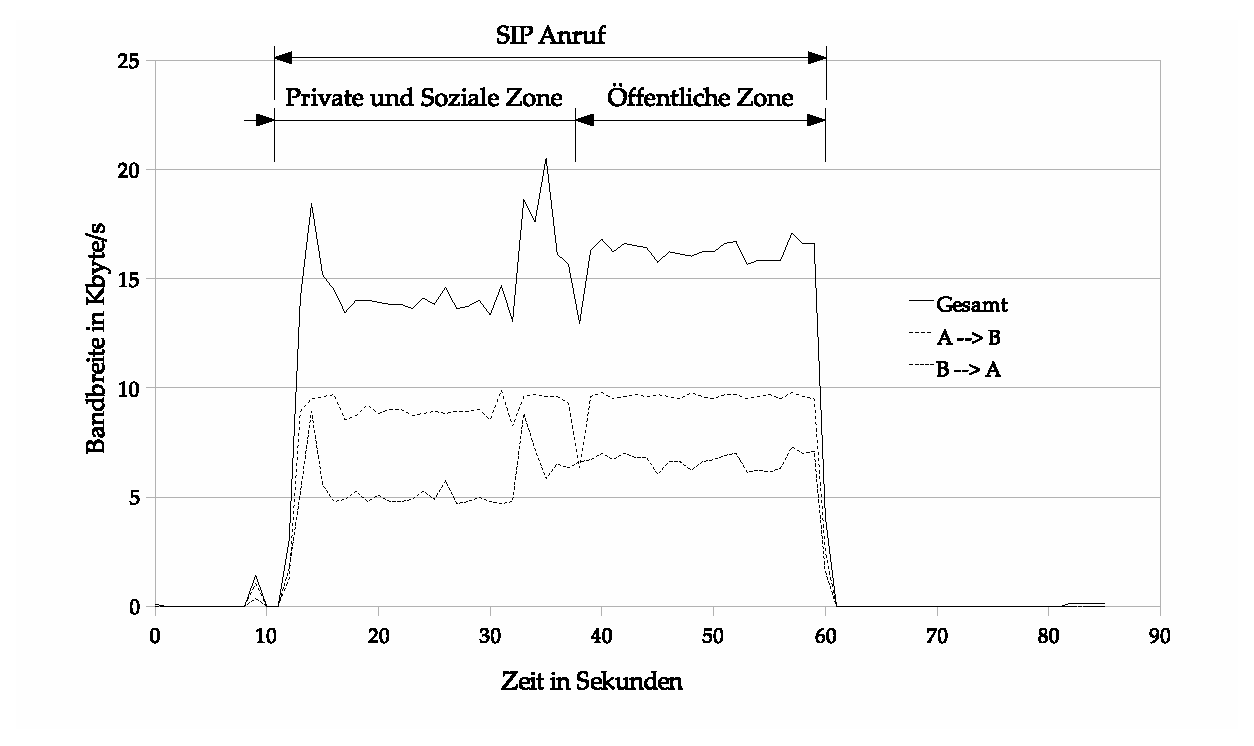
\includegraphics[width=.90\textwidth]{grafiken/ohnevadupdown.eps}
	\caption{Der Up- und Downstream ohne Unterscheidung der Zonen}
	\label{fig:NOVADrtpsip}
\end{figure}

\begin{figure}[tbh]
	\centering
		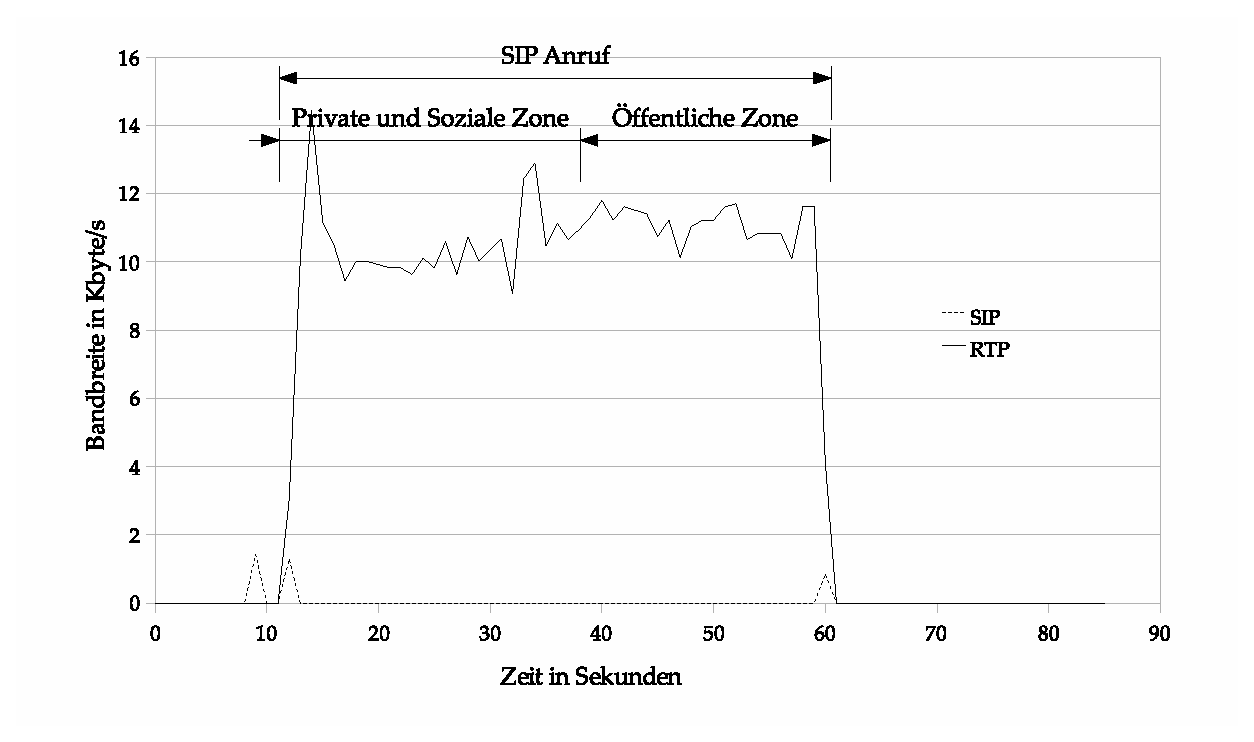
\includegraphics[width=.90\textwidth]{grafiken/ohnevadsiprtp.eps}
		\caption{Signalisierung mit SIP, Audiostrom mit RTP ohne Unterscheidung der Zonen}
	\label{fig:NoVADupdown}
\end{figure}

\begin{figure}[tbh]
	\centering
		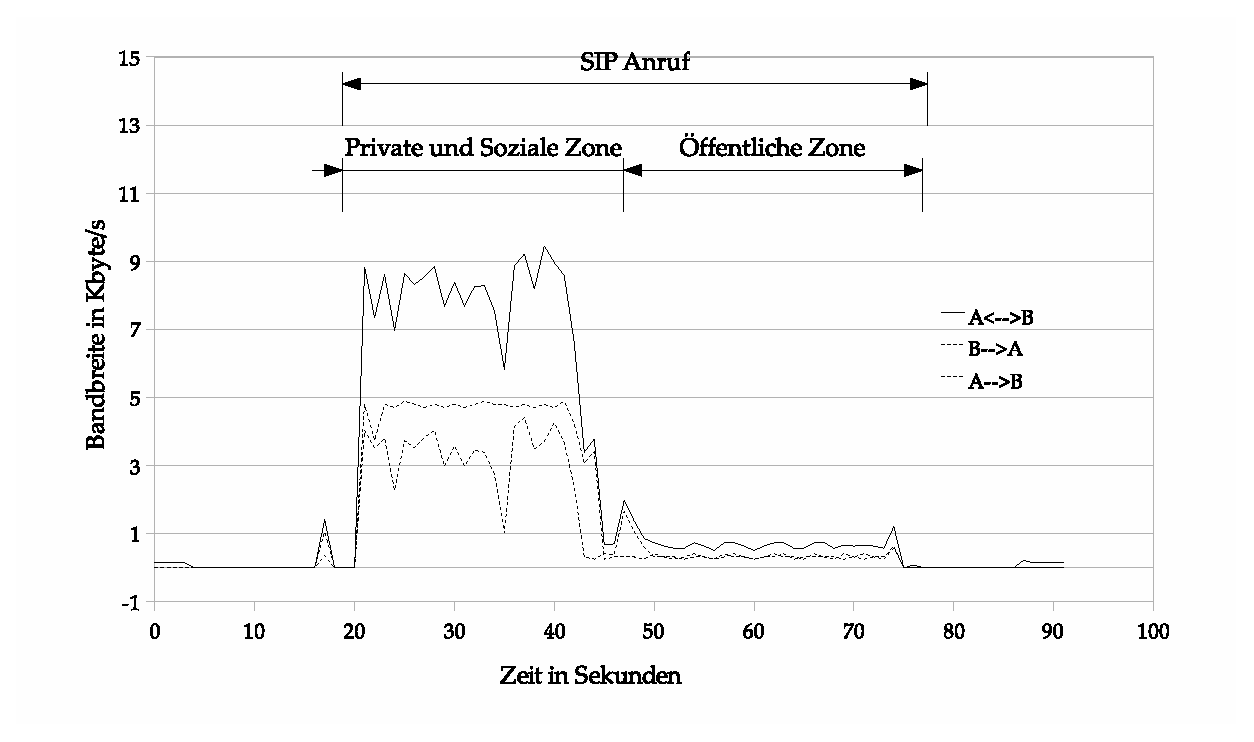
\includegraphics[width=1.00\textwidth]{grafiken/mitvadupdown.eps}
		\caption{Der Up- und Downstream mit der Silcence-Suppression-Technik}
	\label{fig:VADupdown}
\end{figure}

\begin{figure}[tbh]
	\centering
		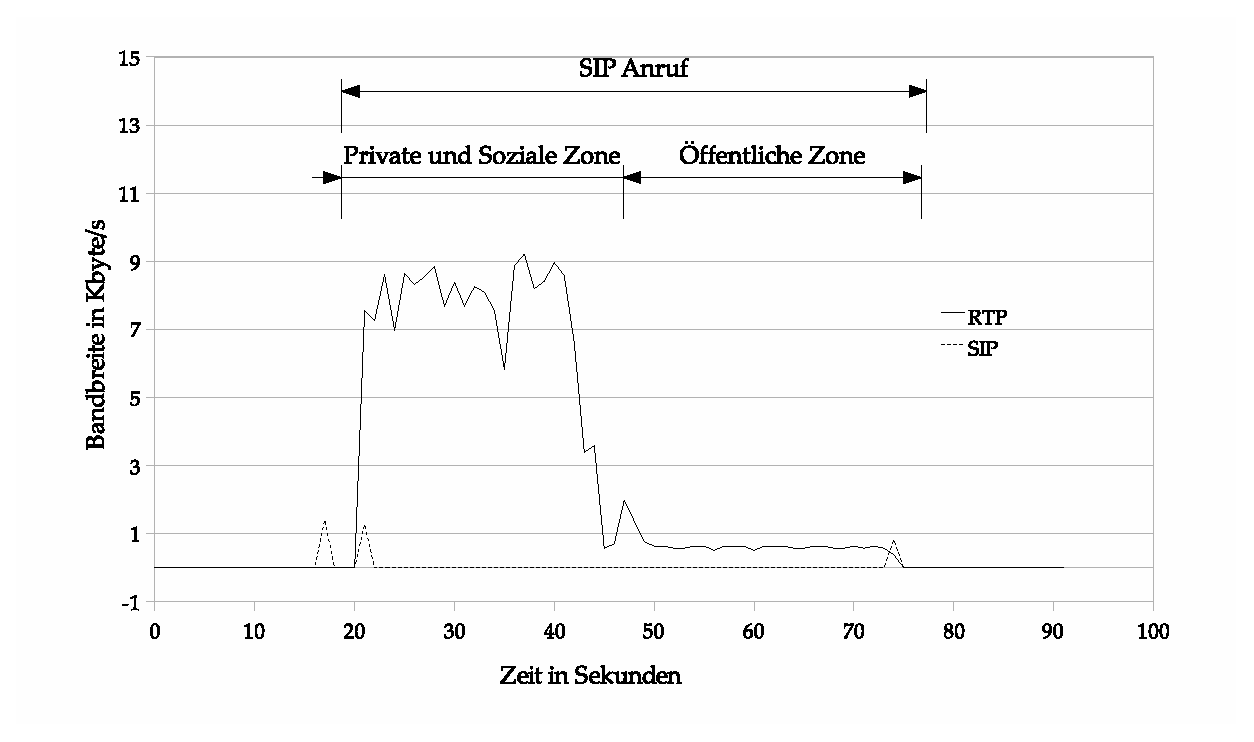
\includegraphics[width=1.00\textwidth]{grafiken/mitvadrtpsip.eps}
		\caption{Der Up- und Downstream mit der Silcence-Suppression-Technik}
	\label{fig:VADrtpsip}
\end{figure}

\begin{figure}[tbh]
	\centering
		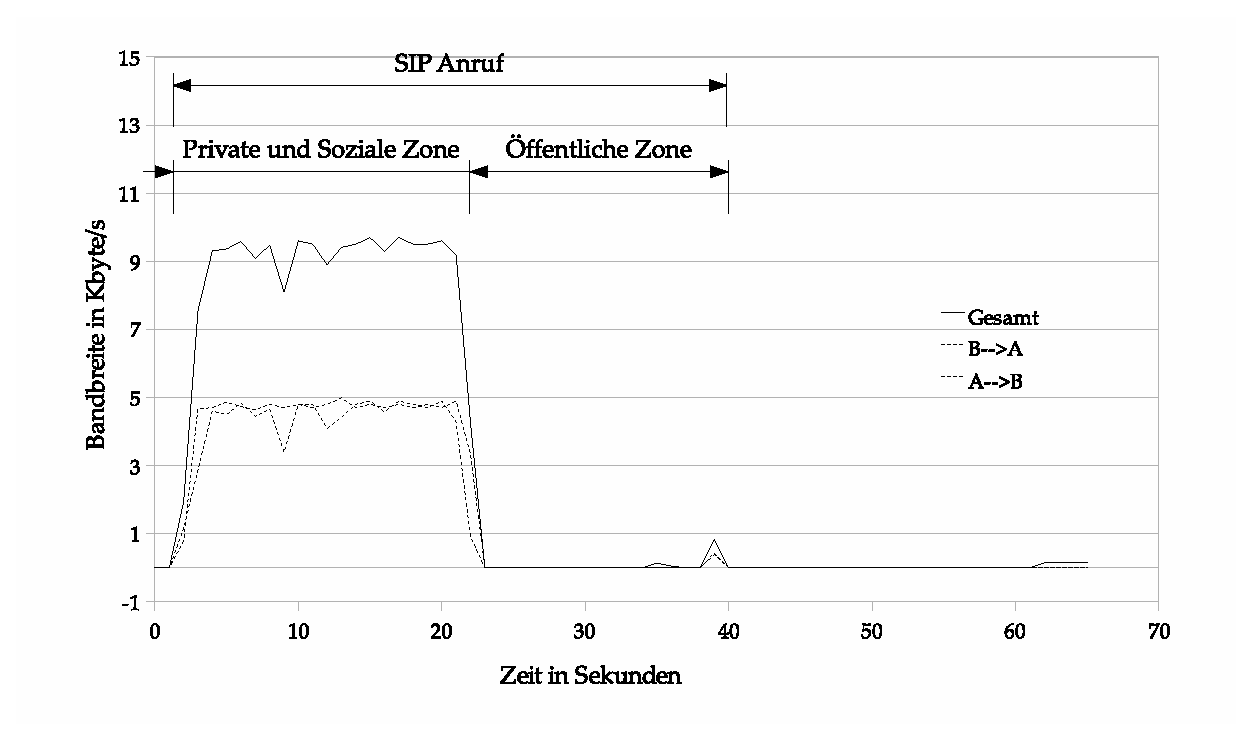
\includegraphics[width=1.00\textwidth]{grafiken/mitholdupanddown.eps}
		\caption{Der Up- und Downstream mit der SIP-Hold-Technik}
	\label{fig:mitholdupanddown}
\end{figure}

\begin{figure}[tbh]
	\centering
		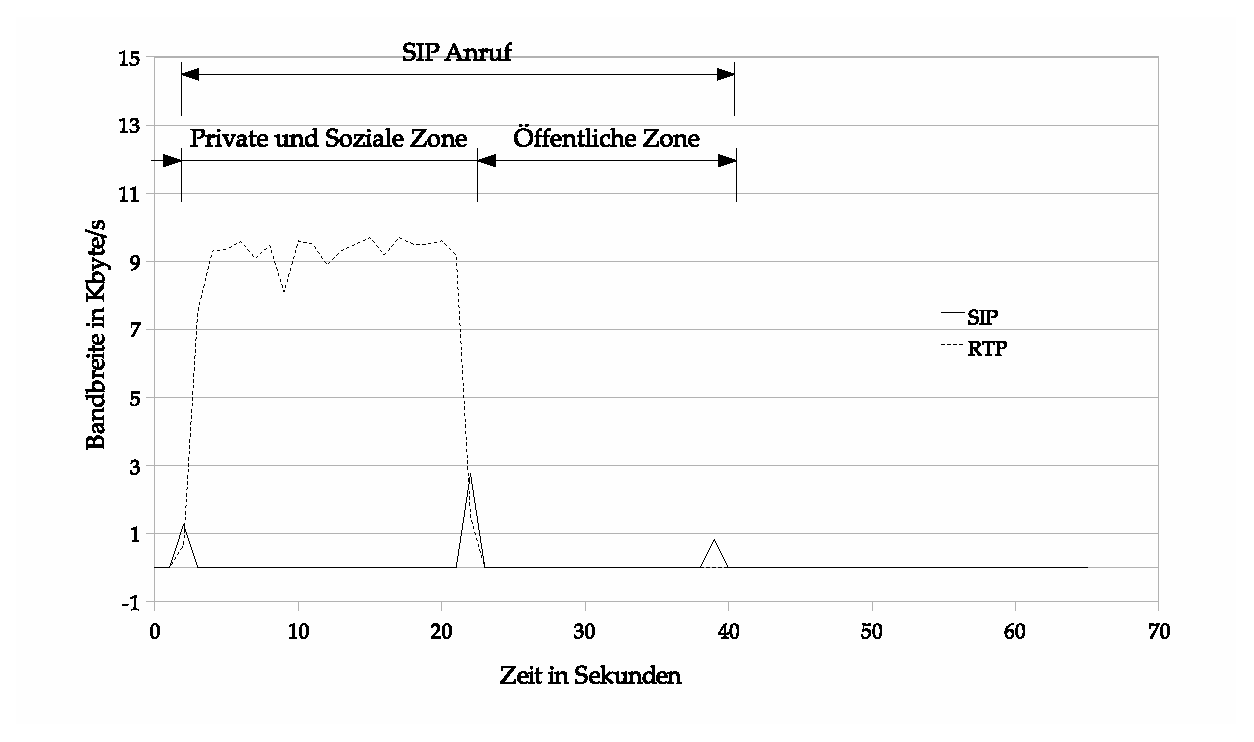
\includegraphics[width=1.00\textwidth]{grafiken/mithold1.eps}
		\caption{Gegen�berstellung des SIP- und RTP-Traffics mit der SIP-HOLD-Technik}
	\label{fig:mithold1}
\end{figure}


\begin{figure}[tbh]
	\centering
		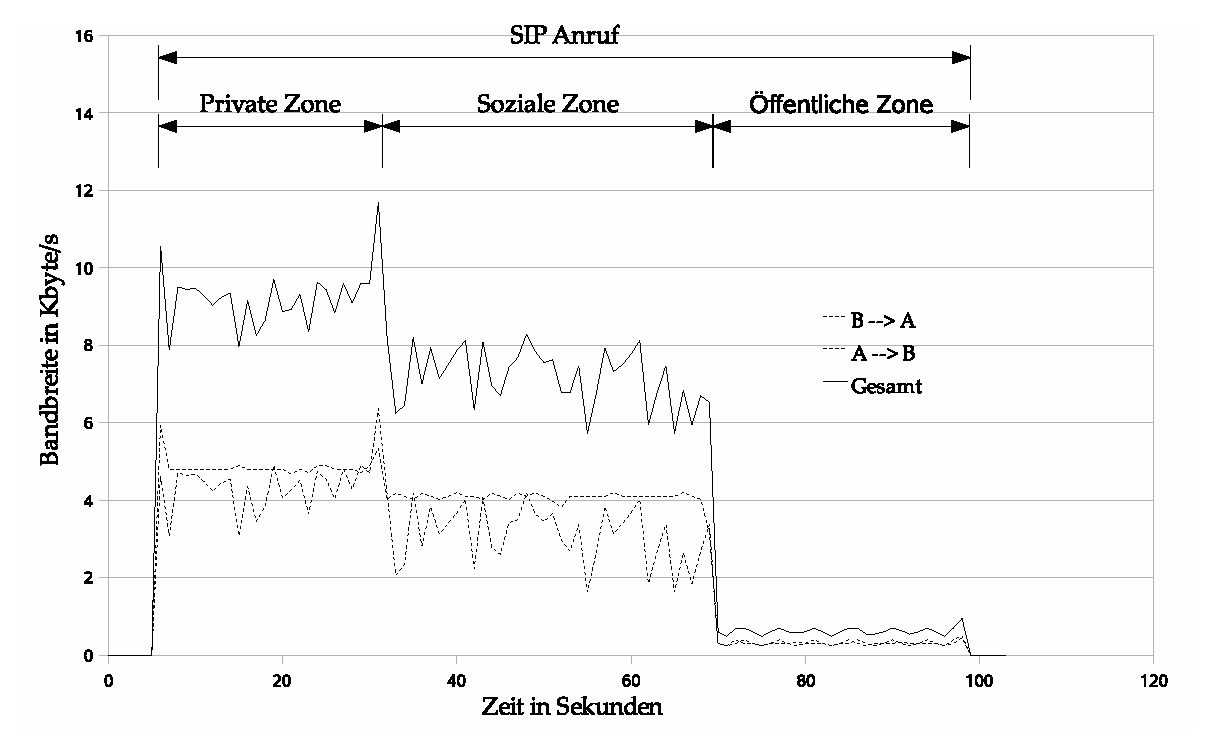
\includegraphics[width=\textwidth]{grafiken/mitvadund2codecs.eps}
		\caption{Speex mit 16 kHz in der privaten Zone und Speex 8 khZ in der sozialen Zone}
	\label{fig:mitvadund2codecs}
\end{figure}

\begin{figure}[tbh]
	\centering
		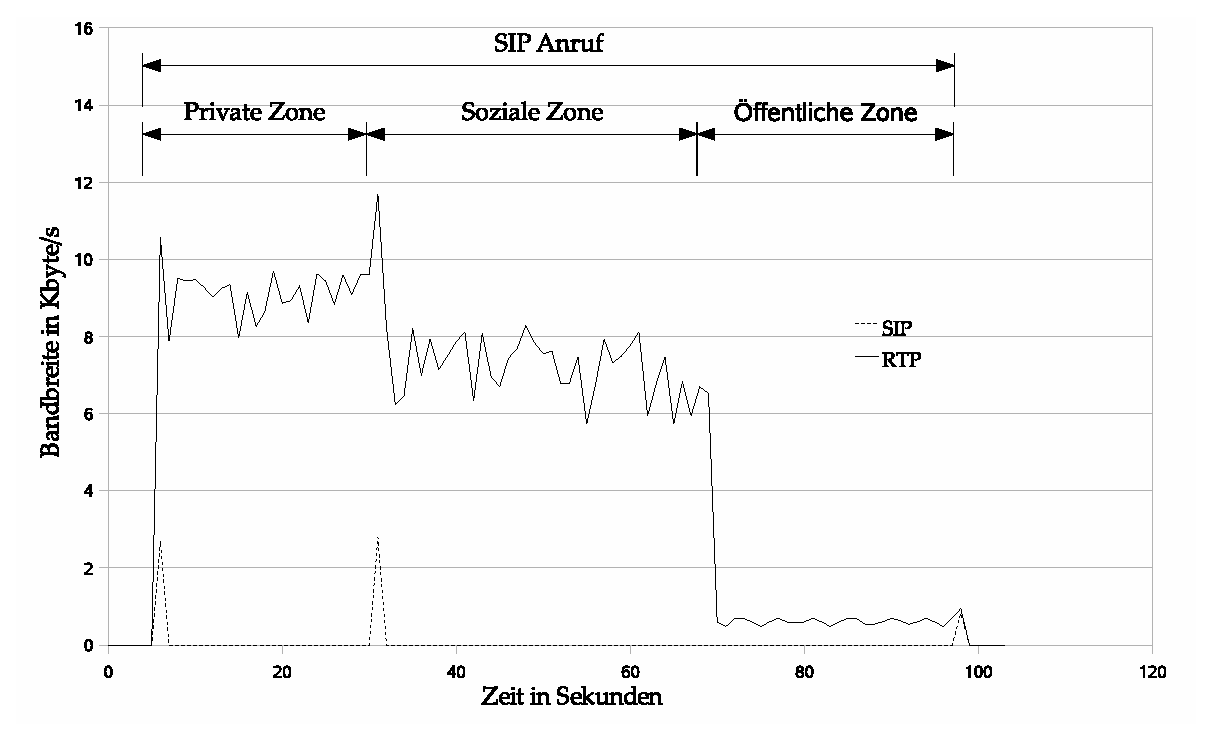
\includegraphics[width=\textwidth]{grafiken/mitvadundrtpsip.eps}
		\caption{Rufauf- und -abbau, sowie Signalisierung eines anderen Codecs mit SIP, Reduktion des Audiostroms mit RTP}
	\label{fig:mitvadundrtpsip}
\end{figure}
%\bibliographystyle{plain}
\bibliographystyle{dinat}
\bibliography{literatur/da}
\chapter*{Eidesstattliche Erkl\"{a}rung}
\thispagestyle{empty}
Ich versichere, dass ich meine Diplomarbeit ohne Hilfe Dritter und ohne Benutzung
anderer als der angegebenen Quellen und Hilfsmittel angefertigt und die den benutzten
Quellen w\"{o}rtlich oder inhaltlich entnommenen Stellen als solche kenntlich gemacht habe.
Diese Arbeit hat in gleicher oder \"{a}hnlicher Form noch keiner Pr\"{u}fungsbeh\"{o}rde
vorgelegen.
\bigskip

\raggedright{Ort, den Datum} \bigskip \bigskip \bigskip

Martin Mustermann
\end{document}